\clearpage
\bookpart{函数空间}{Function Spaces}
\label{part:function-spaces}

\BookPartGuide{%
当一条曲线或一个多变量函数本身成为研究对象时，比较两条函数需要先说明比较哪些位置、怎样累计差异，函数列的极限也未必仍属于原先选定的函数集合。第一章把函数当作空间中的元素，建立范数、完备性与Hilbert空间的正交几何，使误差、极限和正交分量都有明确含义。

第二、三章研究作用在函数上的线性映射。第二章讨论映射怎样传递误差、标量读取怎样表示，以及对偶、弱收敛、伴随和逆映射的稳定性；第三章转向能用有限个方向逼近的紧算子，借谱与奇异值分解积分算子，并判断积分方程的解是否存在、唯一且稳定。

后三章在这些工具上展开。第四章在经典导数失效时用测试函数保存变化信息，建立Sobolev空间及其正则性、紧性与边界迹；第五章研究点值读取连续的Hilbert函数空间，说明核怎样确定空间、表示观测并联系积分谱；第六章比较给定函数的有限逼近与整个函数类的有限覆盖。阅读时应留意每个结论所用的空间、范数和条件：单个函数可以逼近，并不意味着整类函数能被同一组有限代表统一覆盖。}

\chapter{函数空间}
\label{chap:function-spaces}
\label{chap:functional-analysis-and-approximation}

拟合一条曲线时，我们常把候选写成固定基函数的组合$f_m=\sum_{j=1}^mc_j\varphi_j$，并用系数向量的欧氏距离比较两个候选。只要$m$固定、基也固定，这样做没有问题。可是一旦为了提高精度而不断增加项数，系数向量的维数随之改变；同一个函数换一组基，系数也会完全不同。这时“两条函数相差多少”“一列近似是否收敛”“极限还是不是我们要的那类函数”，都不能再靠比较系数回答，而要直接在函数之间建立距离和几何。

本章围绕四个问题展开：哪些函数可以参与线性运算，什么情况下两个函数算作同一个元素？怎样规定两条函数之间的误差？一列彼此越来越接近的函数，极限是否仍在原来的函数集合里？在有了内积之后，能否像在有限维中那样取出最近分量，并用正交方向写出坐标？

第~\ref{sec:fs-elements}节先确定空间的成员和“相等”的含义：逐点运算使函数组成线性空间，积分误差则要求把只在零测集上不同的函数看成同一个元素。第~\ref{sec:fs-norms-completeness}节在这些元素上建立范数、完备性和内积，并用连续斜坡逼近阶跃的例子说明，各项互相接近并不保证极限留在原集合中。这个例子贯穿后文：第~\ref{sec:fs-continuous}节表明同一组连续函数在一致范数下完备，换成平方积分误差就不完备；第~\ref{sec:fs-integral}节因此扩大到可测函数的等价类，构造$L^p$空间并证明它们完备。

有了多种空间，第~\ref{sec:fs-relations}节比较它们：成员何时能从一个空间转入另一个，换一个测度后元素与误差怎样变化，哪些简单函数足以逼近一般成员，以及一致、积分和逐点三种收敛之间能推出什么、不能推出什么。第~\ref{sec:fs-orthogonal}节回到Hilbert空间，证明闭子空间上的正交投影存在且唯一，并用正交系写出展开和截断误差；斜坡与阶跃的例子在这里再次出现，说明闭性缺失时最近点可能不存在。

全章以实值函数为主线，复数情形只在需要时补充约定。所用的测度、积分及其极限定理来自第~\ref{chap:measure-spaces}章，完备性、稠密性和可分性的一般定义来自第~\ref{chap:metric-spaces}章；本章把它们落实到函数上，不重新组织积分论。

% 第1章第1节：函数作为空间元素（线性运算与维数；普通函数与几乎处处等价类）。

\section{函数作为空间元素}
\label{sec:fs-elements}

要比较两条函数、讨论一列函数的极限，先得说清楚参与比较的对象是什么。本节回答两个问题：函数之间怎样做加法和数乘，一个函数集合何时对这些运算封闭；以及在积分误差下，什么样的两个函数应当看成同一个元素。后面所有的范数、点值和极限都沿用这里的约定。

\subsection{函数的线性运算与维数}
\label{sec:fs-linear-structure}

\paragraph{逐点运算}
固定一个非空的输入集合$X$，考虑实值函数$f:X\to\mathbb R$。讨论函数时要分清三个层次：输入位置$x$，函数在该位置的值$f(x)$，以及整个函数$f$。前两者是$X$中的点和实数，第三者是一条完整的对应规则。本章把第三者当作一个“点”来处理。

两个函数的和与一个函数的数乘逐点定义：
\[
 (f+g)(x)=f(x)+g(x),\qquad (cf)(x)=c\,f(x),\qquad x\in X,\ c\in\mathbb R .
\]
每个等式右边都是实数运算，所以交换律、结合律、分配律等线性空间公理在每个$x$处分别成立，从而对整个函数成立；零元素是处处为零的函数，$f$的负元是$x\mapsto-f(x)$。于是全体函数$X\to\mathbb R$组成一个实线性空间。线性空间与线性子空间的一般定义可参考\BookChapterRef{chap:linear-representation}{卷一“线性空间、映射与坐标”章}。

\paragraph{子空间的封闭性检查}
实际使用的通常不是全体函数，而是某个候选集合$V$。要把$V$当作线性子空间，必须逐项核对：零函数在$V$中，$V$中两个成员之和仍在$V$中，成员的数乘仍在$V$中。闭区间$[a,b]$上的连续函数全体$C([a,b])$满足这三条，因为连续函数的和与数乘仍连续；次数不超过$m$的多项式全体$\mathcal P_m$也满足，因为两个这样的多项式相加不会提高次数。更一般地，任意给定函数$\varphi_1,\ldots,\varphi_m$的张成$\operatorname{span}\{\varphi_1,\ldots,\varphi_m\}$总是线性子空间。

由参数描述的函数族却不一定封闭。考虑单个“折线单元”组成的族
\[
 \mathcal R=\{\,x\mapsto a\max(0,x-t):a,t\in\mathbb R\,\},
\]
它只有两个参数。取$f(x)=\max(0,x)$与$g(x)=\max(0,x-1)$，二者都在$\mathcal R$中，但$f+g$在$x=0$和$x=1$各有一个折点，而$\mathcal R$中每个成员至多一个折点，所以$f+g\notin\mathcal R$。宽度固定的神经网络、固定节点数的样条等非线性参数族都有同样的现象：两个成员之和通常需要更多的参数才能表示。这类族可以作为逼近工具（第~\ref{chap:function-approximation}章），但不能直接当作线性空间使用。

\paragraph{输入维数、参数数目与空间维数}
函数空间的维数与输入的维数是两回事。在区间$[a,b]$上，函数$1,x,x^2,\ldots,x^m$线性无关：若$\sum_{k=0}^mc_kx^k=0$对每个$x\in[a,b]$成立，左边是一个在无穷多点取零的多项式，只能所有系数为零。$m$可以任意大，所以$C([a,b])$包含任意多个线性无关的方向，是无限维的，尽管输入只有一个坐标。

参数数目又是第三回事。上面的$\mathcal R$只有两个参数，却不是线性空间，谈不上维数；$\mathcal P_m$是$m+1$维空间，参数数目恰为维数。即使在同一个有限维空间里，坐标也依赖所选的基。例如$x^2$在基$\{1,x,x^2\}$下的系数是$(0,0,1)$，在基$\{1,x,x^2-\tfrac13\}$下的系数是$(\tfrac13,0,1)$。若用系数的欧氏距离衡量误差，同一对函数在两组基下会得到不同的数值；若为提高精度不断增加项数，系数向量更是落在维数不断变化的空间里。因此比较函数需要一个不依赖表示坐标、直接作用于函数本身的误差规则，这就是第~\ref{sec:fs-norms-completeness}节的范数。

\subsection{普通函数与几乎处处等价类}
\label{sec:fs-ae-classes}

\paragraph{零测改值}
逐点运算把每个函数都当作不同的元素：只要某一点的值改变，函数就变了。但若两个函数之间的误差是通过积分累计的，有些改动根本不影响误差。在$[0,1]$上取Lebesgue测度，令$f\equiv0$，而$g$除$g(\tfrac12)=1$外处处为零。单点集的Lebesgue测度为零，零测集上的改动不影响积分（第~\ref{sec:measure-general-structure}节），所以
\[
 \int_0^1|f(x)-g(x)|\,dx=0 .
\]
图~\ref{fig:fs-ae-representatives}显示了这两个函数：作为普通函数它们在$x=\tfrac12$处不同，但任何用积分衡量的误差都看不出差别。

\begin{figure}[!htb]
  \centering
  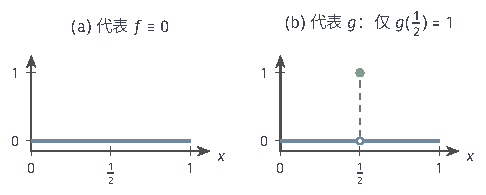
\includegraphics[width=82.2mm]{figures/02-abstract-mathematics/03-function-spaces/tikz/c1-ae-representatives/figure.pdf}
  \caption{同一个几乎处处等价类的两个代表。定义域为$[0,1]$并取Lebesgue测度；(a)中$f\equiv0$，(b)中$g$只在$x=\tfrac12$处取$1$（绿点），空心圈表示$g$在该点不取$0$。单点集测度为零，所以$\int_0^1|f-g|\,dx=0$，二者代表同一个积分空间元素，但它们在$\tfrac12$处的点值不同。}
  \label{fig:fs-ae-representatives}
\end{figure}

\paragraph{等价类与线性运算}
在测度空间$(X,\mathcal A,\mu)$上，对两个可测函数规定
\[
 f\sim_\mu g\quad\Longleftrightarrow\quad \mu(\{x:f(x)\neq g(x)\})=0,
\]
即$f=g$在$\mu$下几乎处处成立。这是一个等价关系：自反与对称是显然的；若$f\sim_\mu g$且$g\sim_\mu h$，则$\{f\neq h\}\subseteq\{f\neq g\}\cup\{g\neq h\}$，两个零测集的并仍是零测集，所以$f\sim_\mu h$。把与$f$几乎处处相等的可测函数全体记为$[f]_\mu$，称为$f$的\term{等价类}（equivalence class），$f$称为它的一个代表。

等价类之间的线性运算借助代表定义：$[f]_\mu+[g]_\mu=[f+g]_\mu$，$c[f]_\mu=[cf]_\mu$。要使这个定义有意义，结果必须不依赖代表的选择。若$f'\sim_\mu f$、$g'\sim_\mu g$，则
\[
 \{f'+g'\neq f+g\}\subseteq\{f'\neq f\}\cup\{g'\neq g\},
\]
右边是零测集，所以$f'+g'\sim_\mu f+g$；数乘同理。于是可测函数的等价类组成一个线性空间，零元素是“几乎处处为零的函数”这一整类。第~\ref{sec:fs-integral}节的$L^p$空间就建立在这样的等价类上。

\paragraph{点值不再自动有意义}
取等价类的代价是：一个类通常没有确定的点值。在Lebesgue测度下每个单点都是零测集，同一类中的代表可以在任意给定的点取任意值，所以“$[f]_\mu$在$x_0$处的值”没有意义。这与测度有关。若某点是原子，即$\mu(\{x_0\})>0$，则同一类的所有代表在$x_0$处必须取同一个值；在计数测度下只有空集是零测集，等价类退化为普通函数。

也不能把等价类当作已经选好了“最好的”代表。在区间上的Lebesgue测度下，若一个类含有连续代表，这个连续代表是唯一的：两个连续函数之差不为零的点组成开集，非空开区间的测度为正，所以两个几乎处处相等的连续函数必定处处相等。但许多类根本没有连续代表（第~\ref{sec:fs-norms-completeness}节的阶跃函数就是一例），而且即使有，从类中读出它的点值也需要另外的论证。本章只固定元素的含义；点值读取何时有良定义、何时连续，由第~\ref{sec:lfo-point-evaluation}小节讨论，点值读取连续的Hilbert函数空间则是第~\ref{chap:rkhs}章的对象。

% 第1章第2节：范数、内积与完备性（函数范数与误差；范数收敛与Banach空间；内积与Hilbert空间）。

\section{范数、内积与完备性}
\label{sec:fs-norms-completeness}

有限维向量的范数与内积在卷一中已经建立，本节把它们用到函数上。定义本身几乎不变，变化在于用途：在无限维空间里，一列彼此越来越接近的元素是否真有极限、极限是否还在原来的集合中，需要逐一检查，而不再像有限维那样自动成立。

\subsection{函数范数与误差}
\label{sec:fs-norms}

\paragraph{两种误差要求}
比较$[0,1]$上的$f(x)=x$与$g(x)=x^2$，至少有两种自然的做法。若关心最坏的位置，可以取最大偏差$\sup_{x}|x-x^2|$；$x-x^2$在$x=\tfrac12$处取最大值，结果为$\tfrac14$。若关心整体的累计偏差，可以取$\int_0^1|x-x^2|\,dx=\tfrac12-\tfrac13=\tfrac16$。两个数都合理，回答的是不同的问题。为了让不同的误差规则共享同一套推理，我们只要求它们满足几条共同的性质。

\begin{definition}[范数]
\label{def:fs-norm}
设$V$是实（或复）线性空间。映射$\|\cdot\|:V\to[0,\infty)$称为$V$上的\term{范数}（norm），若对所有$f,g\in V$与标量$c$，
\begin{enumerate}
 \item 正定性：$\|f\|=0$当且仅当$f=0$；
 \item 齐次性：$\|cf\|=|c|\,\|f\|$；
 \item 三角不等式：$\|f+g\|\leq\|f\|+\|g\|$。
\end{enumerate}
配备了范数的线性空间称为赋范空间。
\end{definition}

三条公理各有用处。正定性保证误差为零当且仅当两个元素相同；齐次性保证把函数整体放大$c$倍时误差也放大$|c|$倍；三角不等式保证两段误差串联起来不超过各自之和，这是后面所有误差估计的基本工具。令$d(f,g)=\|f-g\|$，由三条公理可以直接验证度量公理（定义~\ref{def:metric-space}）：例如$d(f,h)=\|(f-g)+(g-h)\|\leq d(f,g)+d(g,h)$。所以每个赋范空间都是度量空间，第~\ref{chap:metric-spaces}章关于收敛、Cauchy列、闭集和完备性的结论都可以直接使用。

\paragraph{半范数与零方向}
有时一个误差公式满足齐次性和三角不等式，却让某些非零元素的“长度”为零，这样的公式称为\term{半范数}（seminorm）。在$[0,1]$上的全体有界可积函数中，$p(f)=\int_0^1|f|\,dx$就是半范数：上一节的$g=\mathbf 1_{\{1/2\}}$不为零，却有$p(g)=0$。又如在连续可微函数上，$p(f)=\sup_x|f'(x)|$对所有常数函数都取零。

处理零方向有两种办法。一是缩小对象：把$\int_0^1|f|\,dx$限制在$C([0,1])$上，若连续函数$f$在某点$x_0$处$|f(x_0)|>0$，则在$x_0$的一个邻域内$|f|>|f(x_0)|/2$，积分为正，所以在连续函数上它是范数。二是把零长度的元素识别为零，即对半范数为零的方向取商；在积分误差下，这正是第~\ref{sec:fs-ae-classes}小节的几乎处处等价类。第~\ref{sec:metric-pseudometric}节在度量空间中讨论过同样的商构造。无论哪种办法，都不能直接把只满足半范数条件的公式称为原对象上的范数。

\paragraph{系数误差与Gram矩阵}
回到章首的问题：当函数由有限个基函数表示时，函数之间的误差和系数之间的误差是什么关系？取平方积分误差$\|h\|_2^2=\int h^2\,d\mu$。对$f=\sum_jc_j\varphi_j$与$g=\sum_jc'_j\varphi_j$，记$\bm\delta=\bm c-\bm c'$，展开平方并利用积分的线性，
\[
 \|f-g\|_2^2=\int\Bigl(\sum_{i}\delta_i\varphi_i\Bigr)\Bigl(\sum_j\delta_j\varphi_j\Bigr)d\mu
 =\sum_{i,j}\delta_i\delta_j\int\varphi_i\varphi_j\,d\mu
 =\bm\delta^{\top}\bm G\bm\delta,
\]
其中$\bm G_{i,j}=\int\varphi_i\varphi_j\,d\mu$组成\term{Gram矩阵}（Gram matrix）。系数的欧氏距离平方是$\bm\delta^{\top}\bm\delta$，两者相等当且仅当$\bm G=\bm I$，即基函数两两正交且各自的平方积分为$1$。

在$[-1,1]$上取Lebesgue测度与基$\{1,x\}$，$\int1\,dx=2$，$\int x\,dx=0$，$\int x^2\,dx=\tfrac23$，所以$\bm G=\operatorname{diag}(2,\tfrac23)$，函数误差为$2\delta_1^2+\tfrac23\delta_2^2$。系数差$(1,0)$与$(0,1)$的欧氏长度都是$1$，对应的函数误差却分别是$\sqrt2$与$\sqrt{2/3}$。若改在$[0,1]$上使用同一组基，$\bm G=\begin{bmatrix}1&1/2\\1/2&1/3\end{bmatrix}$不再是对角阵，常数方向与线性方向的误差还会相互耦合。平方积分误差在连续函数上确实是范数：正定性的论证与上一段相同，三角不等式由Cauchy--Schwarz不等式得到，下面第~\ref{sec:fs-hilbert}小节在一般内积空间中给出证明。有限维的Gram矩阵、正交化与范数等价，可参考\BookChapterRef{chap:normed-inner-product-spaces}{卷一“赋范空间与内积空间”章}；本章不重建这些结论。

\subsection{范数收敛与Banach空间}
\label{sec:fs-banach}

有了范数，就可以讨论函数列的收敛。设$(f_n)$是赋范空间$V$中的序列，$f\in V$。若$\|f_n-f\|\to0$，称$f_n$\term{依范数收敛}（convergence in norm）到$f$。若对每个$\varepsilon>0$存在$N$，使$m,n\geq N$时$\|f_n-f_m\|<\varepsilon$，称$(f_n)$为范数意义下的\term{Cauchy列}（Cauchy sequence）。由三角不等式$\|f_n-f_m\|\leq\|f_n-f\|+\|f-f_m\|$，收敛列一定是Cauchy列。反过来是否成立，取决于空间。

\paragraph{斜坡逼近阶跃}
在$C([-1,1])$上使用平方积分范数$\|g\|_2=\bigl(\int_{-1}^1g^2\,dx\bigr)^{1/2}$，考察连续斜坡
\[
 g_n(x)=\begin{cases}-1,&x\leq-1/n,\\ nx,&|x|<1/n,\\ 1,&x\geq1/n,\end{cases}\qquad n\geq1 .
\]
图~\ref{fig:fs-ramp-step}画出了$g_2,g_4,g_{16}$：斜坡越来越陡，越来越像阶跃函数$\operatorname{sgn}$。我们先验证它们组成Cauchy列。设$m>n$。在$|x|\geq1/n$处$g_n=g_m$；在$|x|<1/n$处二者同号且绝对值不超过$1$，所以$|g_n-g_m|\leq1$。于是
\[
 \|g_n-g_m\|_2^2\leq\int_{-1/n}^{1/n}1\,dx=\frac2n\to0 .
\]

\begin{figure}[!htb]
  \centering
  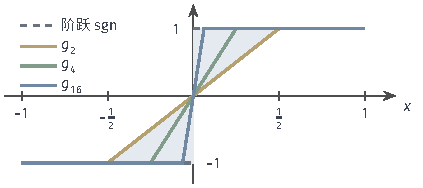
\includegraphics[width=71.6mm]{figures/02-abstract-mathematics/03-function-spaces/tikz/c1-ramp-step/figure.pdf}
  \caption{连续斜坡$g_n$逼近阶跃$\operatorname{sgn}$。$g_n$在$|x|\geq1/n$处与$\operatorname{sgn}$相同，只在宽为$2/n$的区间内线性过渡；阴影是$n=2$时二者的差所在的区域。直接积分得$\int_{-1}^1(g_n-\operatorname{sgn})^2\,dx=\tfrac{2}{3n}\to0$，但$\operatorname{sgn}$在$0$处跳跃，没有连续代表。}
  \label{fig:fs-ramp-step}
\end{figure}

接下来证明这列函数在$C([-1,1])$中没有$\|\cdot\|_2$极限。假设存在连续函数$g$使$\|g_n-g\|_2\to0$。任取$\delta\in(0,1)$，当$n>1/\delta$时$g_n$在$[\delta,1]$上恒为$1$，所以
\[
 \int_\delta^1(1-g)^2\,dx\leq\int_{-1}^1(g_n-g)^2\,dx\to0 .
\]
左边不依赖$n$，只能为零；$(1-g)^2$连续且非负，故$g=1$在$[\delta,1]$上处处成立。同理$g=-1$在$[-1,-\delta]$上成立。由于$\delta$任意，$g$在$(0,1]$上恒为$1$、在$[-1,0)$上恒为$-1$，在$0$处不可能连续，矛盾。

这个例子把两件事分开了：“各项互相接近”是序列自身的性质，“在给定的集合中存在极限”则同时取决于集合和范数。直观上，$g_n$的“极限”应该是阶跃函数，只是阶跃函数不在$C([-1,1])$中。

\begin{definition}[Banach空间]
\label{def:fs-banach}
若赋范空间$V$中的每个Cauchy列都依范数收敛到$V$中的某个元素，称$V$是\term{完备}（complete）的。完备的赋范空间称为\term{Banach空间}（Banach space）。
\end{definition}

按此定义，$(C([-1,1]),\|\cdot\|_2)$不是Banach空间。完备性同时依赖候选集合和范数：第~\ref{sec:fs-uniform-norm}小节将证明同一个$C([-1,1])$在最大偏差范数下完备，第~\ref{sec:fs-lp-completeness}小节则把集合扩大为可测函数的等价类，使平方积分范数下的极限有处可去。

\paragraph{闭子空间与完备性}
在已经完备的空间里，子空间是否完备由它是否闭决定。第~\ref{sec:metric-convergence-completeness}节对度量空间证明了：完备空间的闭子集是完备的，完备子集一定是闭的（定理~\ref{thm:metric-complete-closed}）。用在Banach空间$X$的线性子空间$M$上，这两句话的分工很清楚：$X$的完备性保证$M$中的Cauchy列在$X$中有极限，$M$的闭性保证这个极限没有跑出$M$。

多项式给出一个不闭的子空间。在$[0,1]$上用最大偏差衡量误差，$e^x$的Taylor多项式$p_N(x)=\sum_{k=0}^Nx^k/k!$满足
\[
 \sup_{x\in[0,1]}|e^x-p_N(x)|\leq\frac{e}{(N+1)!}\to0,
\]
这是Lagrange余项的估计。所以$p_N$是多项式空间中的Cauchy列，在连续函数空间中的极限是$e^x$，而$e^x$不是多项式（它的各阶导数都不恒为零）。多项式空间因此不闭，也不完备。第~\ref{sec:apx-polynomial}小节将说明，多项式在这个范数下可以逼近任意连续函数，即它的闭包是整个$C([0,1])$。

\paragraph{完备化}
不完备的空间可以通过添加极限补全。第~\ref{sec:metric-completion}节给出了度量空间的完备化（定理~\ref{thm:metric-completion}）：把Cauchy列$(f_n)$与$(g_n)$在$\|f_n-g_n\|\to0$时视为等价，等价类全体在距离$\lim_n\|f_n-g_n\|$下完备，原空间作为常数列等距地嵌入其中且稠密。对赋范空间，线性运算可以沿Cauchy列延拓：$[(f_n)]+[(g_n)]=[(f_n+g_n)]$，$c[(f_n)]=[(cf_n)]$，范数取$\lim_n\|f_n\|$。这个极限存在，因为$\bigl|\|f_n\|-\|f_m\|\bigr|\leq\|f_n-f_m\|$说明$(\|f_n\|)$是实数Cauchy列；三角不等式和齐次性在极限中保留，所以完备化是Banach空间。

抽象完备化只保证“存在一个完备空间把原空间作为稠密子空间”，并不告诉我们新元素是不是函数、是哪一类函数。把斜坡例子中的“新元素”识别为阶跃函数的等价类，需要第~\ref{sec:fs-integral}节的$L^2$空间和第~\ref{sec:fs-density-separability}小节的稠密性结论。因此本节不预先声称任何给定的函数类已经完备；后面的积分空间、Sobolev空间和核空间都会分别说明完备性从何而来。

\subsection{内积与Hilbert空间}
\label{sec:fs-hilbert}

平方误差还带来一种范数一般没有的结构：可以谈论两个函数是否“垂直”，从而把误差分解成互不干扰的分量。这需要内积。

\begin{definition}[实内积与Hilbert空间]
\label{def:fs-inner-product}
设$V$是实线性空间。映射$\langle\cdot,\cdot\rangle:V\times V\to\mathbb R$称为\term{内积}（inner product），若对所有$f,g,h\in V$与实数$a,b$，
\begin{enumerate}
 \item 对称性：$\langle f,g\rangle=\langle g,f\rangle$；
 \item 线性：$\langle af+bg,h\rangle=a\langle f,h\rangle+b\langle g,h\rangle$；
 \item 正定性：$\langle f,f\rangle\geq0$，且等号当且仅当$f=0$。
\end{enumerate}
记$\|f\|=\sqrt{\langle f,f\rangle}$。在这个范数下完备的内积空间称为\term{Hilbert空间}（Hilbert space）。
\end{definition}

$\|f\|=\sqrt{\langle f,f\rangle}$确实是范数，关键在三角不等式。对任意实数$t$，
\[
 0\leq\|f-tg\|^2=\|f\|^2-2t\langle f,g\rangle+t^2\|g\|^2 .
\]
若$g\neq0$，右边是$t$的二次函数且恒非负，判别式不大于零，得到\term{Cauchy--Schwarz不等式}（Cauchy--Schwarz inequality）
\begin{equation}
 |\langle f,g\rangle|\leq\|f\|\,\|g\| ;
 \label{eq:fs-cauchy-schwarz}
\end{equation}
$g=0$时两边都为零。再由$\|f+g\|^2=\|f\|^2+2\langle f,g\rangle+\|g\|^2\leq(\|f\|+\|g\|)^2$得到三角不等式。正定性与齐次性直接来自内积公理。所以内积空间都是赋范空间，Hilbert空间都是Banach空间。

\paragraph{积分正交}
在$C([-1,1])$上，$\langle f,g\rangle=\int_{-1}^1f(x)g(x)\,dx$是内积：对称性与线性来自积分的性质，正定性的论证与第~\ref{sec:fs-norms}小节相同。它诱导的范数正是平方积分范数$\|\cdot\|_2$。由斜坡例子，这个内积空间不完备，因而不是Hilbert空间；它在第~\ref{sec:fs-integral}节中的扩充$L^2([-1,1])$才是。

若$\langle f,g\rangle=0$，称$f$与$g$\term{正交}（orthogonal）。函数的正交由乘积的整体积分决定，与两条曲线在平面上相交的角度无关。图~\ref{fig:fs-integral-orthogonality}(a)中，$1$与$x$的乘积在正负半区间上的面积各为$\pm\tfrac12$，相加为零，二者正交；(b)中$1$与$x^2$的乘积处处非负，积分为$\tfrac23$，二者不正交。用同样的对称性还可以看出，$[-1,1]$上任何偶函数与任何奇函数都正交，这一事实将在第~\ref{sec:fs-orthonormal-bases}小节用到。

\begin{figure}[!htb]
  \centering
  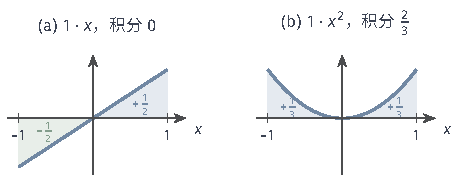
\includegraphics[width=78.2mm]{figures/02-abstract-mathematics/03-function-spaces/tikz/c1-integral-orthogonality/figure.pdf}
  \caption{积分内积下的正交。$[-1,1]$上取Lebesgue测度，曲线是两个函数的乘积，阴影面积带符号累计后即为内积。(a)$1\cdot x$的正负面积各为$\tfrac12$，内积为$0$，$1$与$x$正交；(b)$1\cdot x^2$处处非负，内积为$\tfrac23$，$1$与$x^2$不正交。正交与否只看积分，与曲线的倾角无关。}
  \label{fig:fs-integral-orthogonality}
\end{figure}

\paragraph{复内积的约定}
信号和频域表示需要复值函数。复线性空间上的内积改为共轭对称：$\langle g,f\rangle=\overline{\langle f,g\rangle}$，并且全书统一约定内积对第一个变量共轭线性、对第二个变量线性，即
\[
 \langle af,g\rangle=\bar a\langle f,g\rangle,\qquad \langle f,ag\rangle=a\langle f,g\rangle .
\]
积分内积相应写作$\langle f,g\rangle=\int\overline{f}\,g\,d\mu$。共轭不可省略：在$[-\pi,\pi]$上取$f(x)=e^{ix}$，若不取共轭，$\int f\cdot f\,dx=\int e^{2ix}\,dx=0$，一个非零函数的“长度”会是零；取共轭后$\langle f,f\rangle=\int|e^{ix}|^2\,dx=2\pi$。Cauchy--Schwarz不等式在复情形仍成立（把上面的$t$换成适当的复数），本章主线只用实内积。

\paragraph{范数何时来自内积}
内积诱导的范数满足\term{平行四边形恒等式}（parallelogram identity）
\[
 \|f+g\|^2+\|f-g\|^2=2\|f\|^2+2\|g\|^2,
\]
只需把两边按内积展开，交叉项相互抵消。一般的范数未必满足它。在$C([0,1])$上取最大偏差$\|f\|_\infty=\sup_x|f(x)|$，令$f=1$、$g=x$：$\|f+g\|_\infty=2$，$\|f-g\|_\infty=1$，左边为$5$；$\|f\|_\infty=\|g\|_\infty=1$，右边为$4$。所以最大偏差范数不来自任何内积，$C([0,1])$在这个范数下即使完备，也不是Hilbert空间。“有没有内积”和“是否完备”是两个独立的判断。

\paragraph{有限维直觉的边界}
在有限维空间中，任意两个范数等价，即存在常数$c,C>0$使$c\|v\|_a\leq\|v\|_b\leq C\|v\|_a$，所以范数的选择不影响收敛与完备性。这一结论不能搬到无限维。在$C([0,1])$上，$\|f\|_2\leq\|f\|_\infty$总成立（被积函数不超过$\|f\|_\infty^2$），反方向却没有常数：取$f_n(x)=x^n$，
\[
 \|x^n\|_\infty=1,\qquad \|x^n\|_2=\Bigl(\int_0^1x^{2n}\,dx\Bigr)^{1/2}=\frac{1}{\sqrt{2n+1}}\to0,
\]
比值$\|x^n\|_\infty/\|x^n\|_2=\sqrt{2n+1}$无界。同一个函数集合上的两个范数可以给出完全不同的收敛判断，斜坡例子中的完备性差异也由此而来。

% 第1章第3节：连续函数空间（一致范数与一致收敛；输入域与范数的改变）。

\section{连续函数空间}
\label{sec:fs-continuous}

上一节的定义需要一个完整的例子来落地。本节固定紧区间上的连续函数，配上最大偏差范数，证明得到的是Banach空间。这是最接近一元分析经验的函数空间；随后我们改变输入域和范数，看哪些结论需要重新检查。

\subsection{一致范数与一致收敛}
\label{sec:fs-uniform-norm}

在$C([a,b])$上定义
\begin{equation}
 \|f\|_\infty=\sup_{x\in[a,b]}|f(x)|,
 \label{eq:fs-uniform-norm}
\end{equation}
称为\term{一致范数}（uniform norm）或上确界范数。$|f|$是紧集上的连续函数，由最值定理（定理~\ref{thm:metric-extreme-value}）取到最大值，所以上确界有限，而且实际上是最大值。

范数公理逐条成立。若$\|f\|_\infty=0$，则每一点$|f(x)|\leq0$，$f=0$。齐次性来自$|cf(x)|=|c||f(x)|$在每点成立后取上确界。对三角不等式，每个$x$处都有$|f(x)+g(x)|\leq|f(x)|+|g(x)|\leq\|f\|_\infty+\|g\|_\infty$，右边与$x$无关，对$x$取上确界即得$\|f+g\|_\infty\leq\|f\|_\infty+\|g\|_\infty$。

\paragraph{范数收敛就是一致收敛}
把$\|f_n-f\|_\infty\to0$按定义展开：对每个$\varepsilon>0$存在$N$，使$n\geq N$时$\sup_x|f_n(x)-f(x)|\leq\varepsilon$，即对\emph{所有}$x$同时有$|f_n(x)-f(x)|\leq\varepsilon$。这正是一致收敛：同一个$N$管住全部输入位置。逐点收敛与一致收敛的区别及$x^n$的经典例子，可参考\BookChapterRef{chap:limits-continuity}{卷一“极限与连续”章}。

图~\ref{fig:fs-uniform-tube}给出了几何图像。$\|f_n-f\|_\infty\leq\varepsilon$等价于$f_n$的整条曲线落在以$f$为中心、上下宽$\varepsilon$的带子里，如(a)所示。(b)中的$x^n$在$[0,1)$上逐点趋于$0$，但每条曲线在靠近$x=1$处都会越出零函数周围的带子：$x^4$在$x=0.15^{1/4}\approx0.62$处越出，$x^{12}$推迟到$x=0.15^{1/12}\approx0.85$，越出点随$n$右移，却始终存在。

\begin{figure}[!htb]
  \centering
  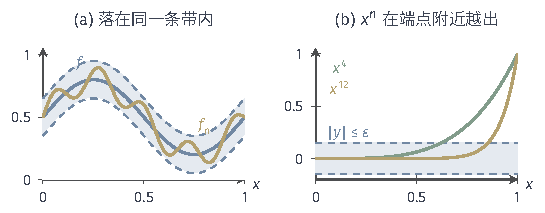
\includegraphics[width=92.2mm]{figures/02-abstract-mathematics/03-function-spaces/tikz/c1-uniform-tube/figure.pdf}
  \caption{一致范数的几何意义。(a)$f(x)=0.5+0.3\sin(2\pi x)$周围宽$\varepsilon=0.15$的带子（浅蓝），$f_n=f+0.1\sin(9\pi x)$整条曲线都在带内，所以$\|f_n-f\|_\infty=0.1\leq\varepsilon$。(b)零函数周围同样宽的带子；$x^4$与$x^{12}$在靠近$x=1$处越出，因为$\|x^n\|_\infty=1$对每个$n$都成立。}
  \label{fig:fs-uniform-tube}
\end{figure}

用一致范数可以把“$x^n$在$[0,1]$上不一致收敛”写成一个具体的数。取$m=2n$，令$t=x^n\in[0,1]$，则
\[
 \|x^n-x^{2n}\|_\infty=\max_{t\in[0,1]}(t-t^2)=\frac14,
\]
最大值在$t=\tfrac12$处取到。这个值不随$n$减小，所以$(x^n)$在$C([0,1])$中连Cauchy列都不是。若把区间缩小到$[0,\tfrac12]$，则$\|x^n\|_\infty=2^{-n}\to0$，一致收敛到零函数。

\paragraph{连续函数空间的完备性}
一致范数下的极限能否留在$C([a,b])$中，是下面这个定理的内容。它的证明包含三个步骤：先构造候选极限，再把逐点收敛加强为一致收敛，最后证明极限连续。三个步骤各有职责，不能从逐点极限直接跳到空间内的收敛。

\begin{theorem}[连续函数空间的完备性]
\label{thm:fs-continuous-complete}
$(C([a,b]),\|\cdot\|_\infty)$是Banach空间。
\end{theorem}

\begin{proof}
设$(f_n)$是一致范数下的Cauchy列。

第一步，逐点构造候选极限。固定$x\in[a,b]$，有$|f_n(x)-f_m(x)|\leq\|f_n-f_m\|_\infty$，所以实数列$(f_n(x))$是Cauchy列。由实数的完备性，它收敛，记极限为$f(x)$。这样得到一个函数$f:[a,b]\to\mathbb R$，但目前只知道$f_n$逐点收敛到它。

第二步，把共同误差界传给极限。给定$\varepsilon>0$，取$N$使$m,n\geq N$时$\|f_n-f_m\|_\infty<\varepsilon$。固定$x$与$n\geq N$，在$|f_n(x)-f_m(x)|<\varepsilon$中令$m\to\infty$，得$|f_n(x)-f(x)|\leq\varepsilon$。这个界与$x$无关，所以$\sup_x|f_n(x)-f(x)|\leq\varepsilon$对所有$n\geq N$成立，即$f_n$一致收敛到$f$。

第三步，证明极限连续。固定$x_0$与$\varepsilon>0$。由第二步取$N$使$\sup_x|f_N(x)-f(x)|<\varepsilon/3$；$f_N$连续，存在$\delta>0$使$|x-x_0|<\delta$时$|f_N(x)-f_N(x_0)|<\varepsilon/3$。对这样的$x$，
\[
 |f(x)-f(x_0)|\leq|f(x)-f_N(x)|+|f_N(x)-f_N(x_0)|+|f_N(x_0)-f(x_0)|<\varepsilon .
\]
所以$f$在$x_0$连续。$x_0$任意，$f\in C([a,b])$；结合第二步，$\|f_n-f\|_\infty\to0$。
\end{proof}

第三步中的“三项误差分解”值得记住：两端的项靠一致收敛统一控制，中间一项靠某个固定的$f_N$的连续性控制。若只有逐点收敛，两端的项无法对邻域内所有$x$同时变小，$x^n$在$[0,1]$上的不连续极限就是例子。

\subsection{输入域与范数的改变}
\label{sec:fs-domain-norm-change}

定理~\ref{thm:fs-continuous-complete}用到了输入域和范数的两项性质：上确界有限，以及一致收敛保持连续。改变输入域或范数时，需要检查的正是这两点。

\paragraph{紧度量空间上的连续函数}
把$[a,b]$换成任意紧度量空间$K$，定义$C(K)$为$K$上的实连续函数，配以$\|f\|_\infty=\sup_{x\in K}|f(x)|$。最值定理在紧度量空间上成立，所以上确界有限；完备性证明的三个步骤只用到实数完备性与度量空间中连续的定义，原样适用。因此$C(K)$也是Banach空间。当$K=\{1,\ldots,n\}$是有限集（任意度量下都紧）时，$C(K)$就是$\mathbb R^n$配最大分量范数。

\paragraph{非紧域与有界连续函数}
在非紧域上，连续函数可能无界：$\mathbb R$上的$f(x)=x$的上确界为$+\infty$，一致“范数”不再是实数。此时改用有界连续函数空间
\[
 C_b(X)=\{f:X\to\mathbb R\ \text{连续}:\ \sup_{x\in X}|f(x)|<\infty\},
\]
配以同样的上确界范数。完备性证明前两步不变。第二步得到的一致误差界还说明极限有界：取定$N$后，对每个$x$都有$|f(x)|\leq\|f_N\|_\infty+\varepsilon$。第三步不依赖紧性。故$C_b(X)$对任意度量空间$X$都是Banach空间。

非紧域上会出现紧区间上没有的现象。在$C_b(\mathbb R)$中取移动的三角形$f_n(x)=\max(0,1-|x-n|)$：每个固定的$x$在$n>|x|+1$后都满足$f_n(x)=0$，所以$f_n$逐点趋于零；但三角形的峰高始终为$1$，$\|f_n\|_\infty=1$，序列不一致收敛。质量没有消失，只是移到了无穷远处。

\paragraph{局部一致收敛}
有些序列在每个有界范围内都一致收敛，在整条实轴上却不收敛。$f_n(x)=x/n$不在$C_b(\mathbb R)$中，但对每个$R>0$，$\sup_{|x|\leq R}|f_n(x)|=R/n\to0$。这种“在每个紧集上一致收敛”称为局部一致收敛，它由一族上确界$\sup_{|x|\leq R}|\cdot|$共同描述，不是单个范数给出的收敛。这类由一族半范数定义的空间不在本章展开；我们只需记住：一致范数关注整个输入域，局部一致收敛只关注每个紧集。

\paragraph{改换范数后的同一集合}
回到同一个集合$C([-1,1])$。在一致范数下它是Banach空间（定理~\ref{thm:fs-continuous-complete}）；换成平方积分范数$\|\cdot\|_2$，第~\ref{sec:fs-banach}小节的斜坡列是Cauchy列却没有连续极限，空间不完备。集合没有变，变的是“接近”的标准。斜坡列在一致范数下不是Cauchy列：对$m>n$，在$x=1/m$处$g_m=1$而$g_n=n/m$，所以$\|g_n-g_m\|_\infty\geq1-n/m$，取$m=2n$即得$\|g_n-g_{2n}\|_\infty\geq\tfrac12$。

平方积分误差关心的是整体偏差，自然的极限是阶跃函数，而它在$0$处的值无关紧要。要让这样的极限有处可去，就需要把成员扩大到可测函数，并且忽略零测集上的差别。这就是下一节积分函数空间的出发点。

% 第1章第4节：积分函数空间（Lp空间与数列空间；Hölder与Minkowski不等式；L∞与本质上界；积分空间的完备性）。

\section{积分函数空间}
\label{sec:fs-integral}

上一节结尾的问题是：平方积分误差下，连续函数的极限可能是阶跃函数这样的不连续函数。本节把误差的累计方式作为出发点，在可测函数的几乎处处等价类上构造两类范数：一类按$p$次幂累计偏差（$1\leq p<\infty$），另一类取忽略零测集后的最大偏差。随后证明三角不等式所需的Hölder与Minkowski不等式，最后证明这些空间都完备。

本节固定测度空间$(X,\mathcal A,\mu)$。可测函数、积分以及单调收敛定理、Fatou引理、控制收敛定理的条件见第~\ref{sec:measure-general-structure}节。

\subsection{$L^p$空间与数列空间}
\label{sec:fs-lp}

\begin{definition}[$L^p$空间]
\label{def:fs-lp}
设$1\leq p<\infty$。若可测函数$f:X\to\mathbb R$满足$\int_X|f|^p\,d\mu<\infty$，称$f$是$p$次可积的。$p$次可积函数的几乎处处等价类全体记为$L^p(\mu)$，并定义
\[
 \bigl\|[f]_\mu\bigr\|_{L^p}=\Bigl(\int_X|f|^p\,d\mu\Bigr)^{1/p}.
\]
当$X$是欧氏空间的子集$\Omega$且$\mu$为Lebesgue测度时，记作$L^p(\Omega)$。
\end{definition}

这个定义需要检查两件事。其一，数值不依赖代表：若$f\sim_\mu g$，则$|f|^p$与$|g|^p$几乎处处相等，零测集上的改动不影响积分，所以两个积分相同。其二，成员对加法封闭。函数$t\mapsto t^p$在$[0,\infty)$上凸（$p\geq1$），所以对$a,b\geq0$有$\bigl(\tfrac{a+b}{2}\bigr)^p\leq\tfrac{a^p+b^p}{2}$，即$(a+b)^p\leq2^{p-1}(a^p+b^p)$。取$a=|f(x)|$、$b=|g(x)|$并积分，
\[
 \int_X|f+g|^p\,d\mu\leq2^{p-1}\Bigl(\int_X|f|^p\,d\mu+\int_X|g|^p\,d\mu\Bigr)<\infty .
\]
数乘的封闭性是显然的，所以$L^p(\mu)$是线性空间。$\|\cdot\|_{L^p}$满足正定性：$\int|f|^p\,d\mu=0$当且仅当$f=0$几乎处处，即$[f]_\mu$是零元素。齐次性直接成立。三角不等式不那么显然，留到第~\ref{sec:fs-holder-minkowski}小节证明。下文在不引起混淆时，用代表$f$代写等价类$[f]_\mu$，并把范数简记为$\|f\|_p$。

\paragraph{不同的$p$衡量不同的整体误差}
$p$越大，局部的大偏差占的比重越大。在$[0,1]$上取窄而高的误差$h=10\cdot\mathbf 1_{[0,0.01]}$：$\|h\|_1=10\times0.01=0.1$，而$\|h\|_2=(100\times0.01)^{1/2}=1$。按绝对偏差累计，这个误差很小；按平方累计，它与“处处偏差为$1$”一样大。选择$p$就是选择怎样为大偏差计价。

用$x^n$可以对照积分误差与最大偏差。在$[0,1]$上，
\[
 \|x^n\|_p=\Bigl(\int_0^1x^{np}\,dx\Bigr)^{1/p}=(np+1)^{-1/p}.
\]
例如$n=10$时，$\|x^{10}\|_1=\tfrac1{11}\approx0.091$，$\|x^{10}\|_2=\tfrac1{\sqrt{21}}\approx0.218$，而$\|x^{10}\|_\infty=1$。图~\ref{fig:fs-xn-norms}(b)画出了三种范数随$n$的变化：两个积分范数都趋于零，$p=2$比$p=1$慢，最大偏差则一直是$1$。原因可以从(a)看出：$x^n$只在越来越窄的一段区间上取大值，积分看到的是这段区间的面积，最大偏差看到的是峰顶。

\begin{figure}[!htb]
  \centering
  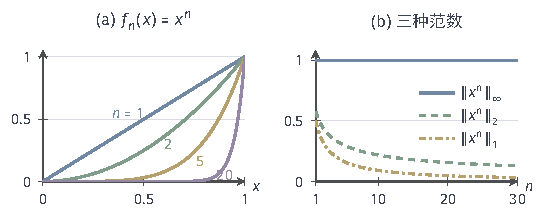
\includegraphics[width=92.3mm]{figures/02-abstract-mathematics/03-function-spaces/tikz/c1-xn-norms/figure.pdf}
  \caption{$x^n$在$[0,1]$上的三种大小。(a)$n=1,2,5,20$时的曲线，函数值集中到右端越来越窄的区间上。(b)三种范数随$n$的变化：$\|x^n\|_\infty=1$，$\|x^n\|_2=(2n+1)^{-1/2}$，$\|x^n\|_1=(n+1)^{-1}$，两个积分范数趋于零，$p=1$下降更快。}
  \label{fig:fs-xn-norms}
\end{figure}

\paragraph{数列空间}
取$X=\mathbb N_+=\{1,2,\ldots\}$与计数测度（每个点的质量为$1$），可测函数就是实数列$x=(x_k)_{k\geq1}$，积分就是求和。此时只有空集是零测集，等价类就是数列本身。$L^p$空间成为
\[
 \ell^p=\Bigl\{x:\ \sum_{k\geq1}|x_k|^p<\infty\Bigr\},\qquad \|x\|_p=\Bigl(\sum_{k\geq1}|x_k|^p\Bigr)^{1/p}.
\]
有限维向量$(x_1,\ldots,x_n)$可以看作后面全为零的数列，$\|x\|_p$就是熟悉的$p$范数，所以$\ell^p$是有限维$p$范数向无限维的自然延伸。数列$x_k=1/k$在$\ell^2$中，因为$\sum_k1/k^2=\pi^2/6$；它不在$\ell^1$中，因为调和级数发散。

\paragraph{平均收敛作为范数收敛}
取概率测度$\mathbb P$，随机变量$Y$的$p$次可积条件就是$\mathbb E|Y|^p<\infty$，范数为$\|Y\|_{L^p(\mathbb P)}=(\mathbb E|Y|^p)^{1/p}$。随机变量的$p$阶平均收敛$\mathbb E|Y_n-Y|^p\to0$因此就是$L^p(\mathbb P)$中的范数收敛。以样本均值为例：设$Y_1,Y_2,\ldots$独立同分布，均值为$m$、方差为$\sigma^2$，则$\bar Y_n=\tfrac1n\sum_{k\leq n}Y_k$满足$\mathbb E(\bar Y_n-m)^2=\sigma^2/n$，即$\|\bar Y_n-m\|_{L^2(\mathbb P)}=\sigma/\sqrt n\to0$。这里只是把已有的平均收敛放进空间结构中，概率收敛的系统理论属于第~\ref{part:probability-spaces}部分，初等的期望与方差计算可参考\BookChapterRef{chap:random-variables}{卷一“随机变量与概率分布”章}。

\subsection{Hölder与Minkowski不等式}
\label{sec:fs-holder-minkowski}

要证明$\|\cdot\|_p$满足三角不等式，需要先控制乘积的积分。设$1<p<\infty$，取$q$满足$\tfrac1p+\tfrac1q=1$，即$q=p/(p-1)$，称$p,q$为\term{共轭指数}（conjugate exponents）。$p=2$时$q=2$；$p=3$时$q=\tfrac32$。

\begin{lemma}[Young不等式]
\label{lem:fs-young}
设$1<p<\infty$，$q$为其共轭指数。对任意$a,b\geq0$，
\[
 ab\leq\frac{a^p}{p}+\frac{b^q}{q},
\]
等号当且仅当$a^p=b^q$。
\end{lemma}

\begin{proof}
固定$b\geq0$，考察$F(s)=\tfrac{s^p}{p}-bs$，$s\geq0$。$F'(s)=s^{p-1}-b$在$s_*=b^{1/(p-1)}$处为零，$s<s_*$时为负、$s>s_*$时为正，所以$F$在$s_*$处取最小值。由$p/(p-1)=q$得$s_*^p=b^q$，于是
\[
 F(s_*)=\frac{b^q}{p}-b\cdot b^{q/p}=\frac{b^q}{p}-b^q=-\frac{b^q}{q},
\]
其中用了$1+q/p=q$。所以$F(a)\geq-b^q/q$，移项即得不等式；等号当且仅当$a=s_*$，即$a^p=b^q$。
\end{proof}

这个不等式有一幅面积图像。共轭条件等价于$(p-1)(q-1)=1$，所以曲线$s=t^{p-1}$也可以写成$t=s^{q-1}$。图~\ref{fig:fs-young-area}中，曲线下方从$0$到$a$的面积是$\int_0^at^{p-1}\,dt=a^p/p$（蓝色），曲线左方从$0$到$b$的面积是$\int_0^bs^{q-1}\,ds=b^q/q$（绿色）。两块区域合起来盖住了矩形$[0,a]\times[0,b]$，所以面积之和不小于$ab$；只有当曲线恰好穿过矩形的右上角，即$b=a^{p-1}$时，两块区域才不多不少地拼成矩形。

\begin{figure}[!htb]
  \centering
  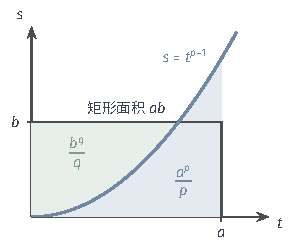
\includegraphics[width=49.6mm]{figures/02-abstract-mathematics/03-function-spaces/tikz/c1-young-area/figure.pdf}
  \caption{Young不等式的面积解释，取$p=3$、$q=\tfrac32$、$a=1$、$b=0.6$。曲线为$s=t^{2}$；蓝色区域面积$a^p/p=\tfrac13$，绿色区域面积$b^q/q\approx0.310$，二者覆盖面积为$ab=0.6$的矩形，多出的部分是曲线在矩形上方的蓝色尖角。}
  \label{fig:fs-young-area}
\end{figure}

\begin{theorem}[Hölder不等式]
\label{thm:fs-holder}
设$1<p<\infty$，$q$为其共轭指数，$f,g$可测。则
\[
 \int_X|fg|\,d\mu\leq\|f\|_p\,\|g\|_q ,
\]
其中右边允许取$+\infty$。特别地，$f\in L^p(\mu)$、$g\in L^q(\mu)$时$fg\in L^1(\mu)$。
\end{theorem}

\begin{proof}
若右边为$+\infty$，无需证明。若$\|f\|_p=0$，则$f=0$几乎处处，$fg=0$几乎处处，左边为零；$\|g\|_q=0$同理。下设$0<\|f\|_p,\|g\|_q<\infty$。在Young不等式中逐点取$a=|f(x)|/\|f\|_p$、$b=|g(x)|/\|g\|_q$，得
\[
 \frac{|f(x)g(x)|}{\|f\|_p\|g\|_q}\leq\frac{|f(x)|^p}{p\|f\|_p^p}+\frac{|g(x)|^q}{q\|g\|_q^q}.
\]
两边积分，右边等于$\tfrac1p+\tfrac1q=1$，再乘以$\|f\|_p\|g\|_q$即得结论。
\end{proof}

归一化这一步的作用是把两个任意大小的函数缩放到“单位大小”，使Young不等式右边的两项积分后恰好凑成$1$。由证明还可以读出等号条件：在每一点都需要$a^p=b^q$，即$|f|^p$与$|g|^q$几乎处处成比例。在$[0,1]$上取$f=x$、$g=x^2$、$p=3$、$q=\tfrac32$：$|f|^p=x^3=|g|^q$，左边$\int_0^1x^3\,dx=\tfrac14$，右边$\|x\|_3\|x^2\|_{3/2}=(\tfrac14)^{1/3}(\tfrac14)^{2/3}=\tfrac14$，等号成立。若取$f=1$、$g=x$、$p=q=2$，左边$\tfrac12$，右边$1\cdot(\tfrac13)^{1/2}\approx0.577$，不等式是严格的。

\begin{theorem}[Minkowski不等式]
\label{thm:fs-minkowski}
设$1\leq p<\infty$，$f,g\in L^p(\mu)$。则$\|f+g\|_p\leq\|f\|_p+\|g\|_p$。因此$(L^p(\mu),\|\cdot\|_p)$是赋范空间。
\end{theorem}

\begin{proof}
$p=1$时，对逐点不等式$|f+g|\leq|f|+|g|$积分即可。设$1<p<\infty$。由第~\ref{sec:fs-lp}小节，$f+g\in L^p$，所以$\int|f+g|^p\,d\mu<\infty$。若它为零，结论平凡，下设它为正。

先把$p$次幂拆成两项：
\[
 |f+g|^p=|f+g|^{p-1}|f+g|\leq|f+g|^{p-1}|f|+|f+g|^{p-1}|g| .
\]
再对每一项用Hölder不等式。由$(p-1)q=p$，$|f+g|^{p-1}$的$q$次积分为$\int|f+g|^p\,d\mu$，所以
\[
 \int|f+g|^{p-1}|f|\,d\mu\leq\Bigl(\int|f+g|^p\,d\mu\Bigr)^{1/q}\|f\|_p ,
\]
第二项同理。两式相加，
\[
 \int|f+g|^p\,d\mu\leq\Bigl(\int|f+g|^p\,d\mu\Bigr)^{1/q}\bigl(\|f\|_p+\|g\|_p\bigr).
\]
左右同除以$(\int|f+g|^p\,d\mu)^{1/q}$（它有限且为正），由$1-\tfrac1q=\tfrac1p$得$\|f+g\|_p\leq\|f\|_p+\|g\|_p$。
\end{proof}

证明中两处条件都不能省：除法要求$\int|f+g|^p\,d\mu$有限且为正，前者来自第~\ref{sec:fs-lp}小节的封闭性估计，后者单独处理。

\paragraph{$0<p<1$时三角不等式失效}
公式$(\int|f|^p\,d\mu)^{1/p}$对$0<p<1$也能计算，但它不是范数。取两点集$\{1,2\}$上的计数测度，$x=(1,0)$、$y=(0,1)$，则$\|x\|_p=\|y\|_p=1$，而
\[
 \|x+y\|_p=(1^p+1^p)^{1/p}=2^{1/p}>2=\|x\|_p+\|y\|_p .
\]
$p=\tfrac12$时左边等于$4$。几何上，范数的单位球$\{v:\|v\|\leq1\}$必定是凸集：若$\|u\|,\|v\|\leq1$，则$\|tu+(1-t)v\|\leq t\|u\|+(1-t)\|v\|\leq1$。图~\ref{fig:fs-unit-balls}画出了平面上$\{|x_1|^p+|x_2|^p\leq1\}$的边界：$p=1,2,\infty$时分别是菱形、圆和正方形，都是凸的；$p=\tfrac12$时边界向内凹，$(1,0)$与$(0,1)$的中点$(\tfrac12,\tfrac12)$满足$2(\tfrac12)^{1/2}\approx1.41>1$，落在集合之外。这正是三角不等式失效的几何表现。

\begin{figure}[!htb]
  \centering
  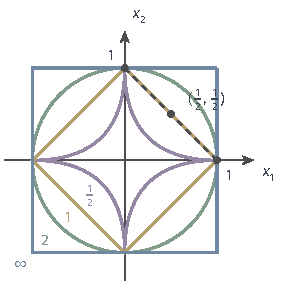
\includegraphics[width=48.6mm]{figures/02-abstract-mathematics/03-function-spaces/tikz/c1-unit-balls/figure.pdf}
  \caption{平面上集合$\{|x_1|^p+|x_2|^p\leq1\}$的边界，曲线旁的数字为$p$；$p=\infty$时为$\max(|x_1|,|x_2|)\leq1$。$p\geq1$时集合是凸的；$p=\tfrac12$时边界内凹，$(1,0)$与$(0,1)$连线的中点$(\tfrac12,\tfrac12)$落在集合外，对应的公式不满足三角不等式。}
  \label{fig:fs-unit-balls}
\end{figure}

\paragraph{$L^2$上的内积}
$p=2$时共轭指数也是$2$，Hölder不等式说明$\int|fg|\,d\mu\leq\|f\|_2\|g\|_2<\infty$，所以
\[
 \langle f,g\rangle=\int_Xfg\,d\mu,\qquad f,g\in L^2(\mu)
\]
有定义，且不依赖代表。对称性与线性来自积分的性质，正定性来自“$\int f^2\,d\mu=0$当且仅当$f=0$几乎处处”。它诱导的范数正是$\|\cdot\|_2$。因此$L^2(\mu)$是内积空间；等第~\ref{sec:fs-lp-completeness}小节证明完备性后，它就是Hilbert空间。

\subsection{$L^\infty$与本质上界}
\label{sec:fs-linfty}

最大偏差也要适应“忽略零测集”的约定。普通上确界会被单个点的值左右，而等价类中的代表可以在零测集上任意改值，所以需要一个只看“几乎处处”的上界。

\begin{definition}[本质上确界与$L^\infty$]
\label{def:fs-linfty}
对可测函数$f$，定义
\[
 \|f\|_\infty=\inf\{M\geq0:\ |f|\leq M\ \text{在}\ \mu\ \text{下几乎处处成立}\},
\]
称为$|f|$的\term{本质上确界}（essential supremum），约定空集的下确界为$+\infty$。本质上确界有限的可测函数称为本质有界的；其几乎处处等价类全体记为$L^\infty(\mu)$。
\end{definition}

先看下确界能否取到。记$M_0=\|f\|_\infty<\infty$，对每个正整数$k$，集合$\{|f|>M_0+1/k\}$是零测集；它们的并$\{|f|>M_0\}$是可数个零测集之并，仍为零测集。所以$|f|\leq\|f\|_\infty$几乎处处成立，下确界是可以达到的。由此也看出数值不依赖代表：若$g\sim_\mu f$，则$\{|g|>M\}\subseteq\{|f|>M\}\cup\{f\neq g\}$，两类函数的本质上界相同。

本质上确界与普通上确界可以相差很远。在$[0,1]$上取Lebesgue测度，令$f(x)=x$，但把$f(\tfrac12)$改为$2$。普通上确界是$2$，而$|f|\leq1$只在单点$\{\tfrac12\}$外成立，所以本质上确界是$1$，如图~\ref{fig:fs-essential-sup}所示。更极端地，有理点示性函数$\mathbf 1_{\mathbb Q\cap[0,1]}$的普通上确界是$1$，本质上确界是$0$，因为有理点只有可数个，组成零测集。这也说明：$\|f\|_\infty\leq M$只保证某个零测集之外处处$|f|\leq M$，并不保证类中任意一个代表在每一点都受这个界控制。若$f$在区间上连续，则$\{|f|>M\}$是开集，非空即有正测度，所以连续函数的本质上确界等于普通上确界。

\begin{figure}[!htb]
  \centering
  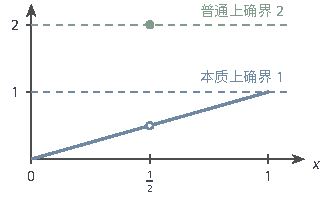
\includegraphics[width=56.1mm]{figures/02-abstract-mathematics/03-function-spaces/tikz/c1-essential-sup/figure.pdf}
  \caption{本质上确界忽略零测集。$[0,1]$上取Lebesgue测度，$f(x)=x$，只把$f(\tfrac12)$改为$2$（绿点，空心圈为原值）。普通上确界被这一个点抬到$2$；单点测度为零，本质上确界仍为$1$。}
  \label{fig:fs-essential-sup}
\end{figure}

\paragraph{范数公理与积分配对}
$\|\cdot\|_\infty$在$L^\infty(\mu)$上是范数，论证的关键是把例外集合并成一个零测集。正定性：若$\|f\|_\infty=0$，由上一段$|f|\leq0$几乎处处，即$f=0$几乎处处。齐次性由$|cf|=|c||f|$得到。三角不等式：$|f|\leq\|f\|_\infty$在零测集$N_f$外成立，$|g|\leq\|g\|_\infty$在零测集$N_g$外成立，于是在$N_f\cup N_g$之外$|f+g|\leq\|f\|_\infty+\|g\|_\infty$，例外集仍是零测集。

$L^\infty$与$L^1$之间有一个自然的积分配对，它是Hölder不等式在端点$p=1$、$q=\infty$的形式：由$|fg|\leq|f|\,\|g\|_\infty$几乎处处成立并积分，
\[
 \int_X|fg|\,d\mu\leq\|f\|_1\,\|g\|_\infty .
\]
约定$\tfrac1\infty=0$后，Hölder不等式对所有共轭指数对$1\leq p\leq\infty$都成立。第~\ref{sec:lfo-lp-dual}小节将从这个配对出发研究$L^p$上的线性泛函。

\paragraph{有界数列空间}
取$\mathbb N_+$上的计数测度，只有空集零测，本质上确界就是普通上确界，得到有界数列空间$\ell^\infty=\{x:\sup_k|x_k|<\infty\}$。常数列$(1,1,1,\ldots)$在$\ell^\infty$中，却不在任何$\ell^p$（$p<\infty$）中。第~\ref{sec:fs-density-separability}小节将看到，$\ell^\infty$与$L^\infty([0,1])$都“太大”，无法用可数个元素逼近；第~\ref{sec:lfo-weak-star}小节则会在$L^\infty$上使用另一种更弱的收敛。

\subsection{积分空间的完备性}
\label{sec:fs-lp-completeness}

现在回答本节开头的问题：积分误差下的Cauchy列是否一定有极限？下面的定理对所有$1\leq p\leq\infty$给出肯定回答，但有限$p$与$p=\infty$的证明方式不同，不能把一个套到另一个上。

\begin{theorem}[积分空间的完备性]
\label{thm:fs-lp-complete}
对任意测度空间与$1\leq p\leq\infty$，$L^p(\mu)$是Banach空间。特别地，$L^2(\mu)$是Hilbert空间。
\end{theorem}

\begin{proof}
先设$1\leq p<\infty$，$(f_n)$是$L^p$中的Cauchy列。证明分五步：抽出快速子列，构造控制函数，定义候选极限，证明子列收敛，最后回到整列。

第一步，抽取相邻差可求和的子列。由Cauchy条件，可以递归地取$n_1<n_2<\cdots$，使$m,n\geq n_k$时$\|f_n-f_m\|_p<2^{-k}$。于是$\|f_{n_{k+1}}-f_{n_k}\|_p<2^{-k}$，$\sum_k\|f_{n_{k+1}}-f_{n_k}\|_p<\infty$。取定各项的可测代表。

第二步，构造控制函数。令
\[
 S_m=|f_{n_1}|+\sum_{k=1}^m|f_{n_{k+1}}-f_{n_k}|,\qquad S=\lim_{m\to\infty}S_m\in[0,\infty].
\]
由Minkowski不等式，$\|S_m\|_p\leq\|f_{n_1}\|_p+\sum_k\|f_{n_{k+1}}-f_{n_k}\|_p=:C<\infty$，界与$m$无关。$S_m^p$逐点单调上升到$S^p$，由单调收敛定理，$\int S^p\,d\mu=\lim_m\int S_m^p\,d\mu\leq C^p$。所以$S\in L^p$，特别地$S<\infty$几乎处处。

第三步，定义候选极限。在$\{S<\infty\}$上，级数$f_{n_1}+\sum_k(f_{n_{k+1}}-f_{n_k})$绝对收敛，其部分和恰为$f_{n_{k+1}}$；令$f$为其和，在零测集$\{S=\infty\}$上令$f=0$。$f$是可测函数列的几乎处处极限，因而可测；$|f|\leq S$，所以$f\in L^p$。至此子列$f_{n_j}\to f$几乎处处。

第四步，证明子列依范数收敛。固定$j$，在$\{S<\infty\}$上$f-f_{n_j}=\lim_{m\to\infty}(f_{n_m}-f_{n_j})$。由Fatou引理与Minkowski不等式，
\[
 \int|f-f_{n_j}|^p\,d\mu\leq\liminf_{m\to\infty}\int|f_{n_m}-f_{n_j}|^p\,d\mu
 \leq\Bigl(\sum_{k\geq j}\|f_{n_{k+1}}-f_{n_k}\|_p\Bigr)^p,
\]
右边是收敛级数的尾和的$p$次方，趋于零。所以$\|f_{n_j}-f\|_p\to0$。

第五步，回到整列。给定$\varepsilon>0$，取$N$使$m,n\geq N$时$\|f_n-f_m\|_p<\varepsilon$，再取$j$使$n_j\geq N$且$\|f_{n_j}-f\|_p<\varepsilon$。则$n\geq N$时$\|f_n-f\|_p\leq\|f_n-f_{n_j}\|_p+\|f_{n_j}-f\|_p<2\varepsilon$。

再设$p=\infty$。取$L^\infty$中的Cauchy列$(f_n)$的代表。对每对$m,n$，$|f_n-f_m|\leq\|f_n-f_m\|_\infty$在某个零测集$E_{m,n}$之外成立。令$E=\bigcup_{m,n}E_{m,n}$，它是可数个零测集之并，仍为零测集。在$X\setminus E$上，所有这些不等式同时成立，所以$(f_n)$在$X\setminus E$上一致Cauchy。与定理~\ref{thm:fs-continuous-complete}的前两步相同，$f_n$在$X\setminus E$上一致收敛到某个函数$f$；在$E$上令$f=0$。$f$是可测函数列在$X\setminus E$上的逐点极限，因而可测；$\sup_{x\notin E}|f_n(x)-f(x)|\to0$给出$\|f_n-f\|_\infty\to0$。取$n_0$使$\|f_{n_0}-f\|_\infty\leq1$，则$\|f\|_\infty\leq\|f_{n_0}\|_\infty+1<\infty$，所以$f\in L^\infty$。

最后，$L^2$的范数由内积诱导，完备后即为Hilbert空间。
\end{proof}

两种证明的差别值得对照。有限$p$的论证没有一致性可用，只能先抽子列，借$S\in L^p$得到几乎处处收敛，再用Fatou引理把逐点信息转为积分信息；$p=\infty$的论证则把可数个例外集合并成一个零测集，在其补集上做一致收敛，与连续函数空间的证明如出一辙。

证明的前三步还给出了一个单独有用的结论，第~\ref{sec:fs-convergence-modes}小节比较收敛方式时会用到。

\begin{theorem}[范数收敛的几乎处处收敛子列]
\label{thm:fs-ae-subsequence}
设$1\leq p<\infty$，$f_n\to f$在$L^p(\mu)$中成立。则存在子列$(f_{n_k})$使$f_{n_k}\to f$几乎处处成立。
\end{theorem}

\begin{proof}
收敛列是Cauchy列。定理~\ref{thm:fs-lp-complete}证明的前四步构造出子列和函数$\tilde f$，使$f_{n_k}\to\tilde f$几乎处处且在$L^p$中成立。$L^p$极限唯一，所以$\tilde f=f$几乎处处。
\end{proof}

回到斜坡例子。在$L^2([-1,1])$中，$\operatorname{sgn}$的等价类是一个合法元素，并且
\[
 \|g_n-\operatorname{sgn}\|_2^2=2\int_0^{1/n}(1-nx)^2\,dx=\frac{2}{3n}\to0 .
\]
所以在$L^2$中，斜坡列有了极限。$\operatorname{sgn}$在$0$处取什么值无关紧要，这正是取等价类的用意。

% 第1章第5节：空间之间的关系（包含关系与范数比较；换测度后的元素与范数；稠密子集与可分性；收敛方式与误差传递）。

\section{空间之间的关系}
\label{sec:fs-relations}

前两节分别构造了连续函数空间、$L^p$空间和数列空间。同一个函数常常同时属于几个空间，同一个误差也可以在几种范数下计算。本节分四个问题比较它们：成员能否从一个空间转入另一个空间；换一个测度后元素与范数怎样变化；能否用简单的、可数的对象逼近一般成员；以及不同意义下的收敛能互相推出什么。每个问题都先固定比较的对象，再给出足够的条件。

\subsection{包含关系与范数比较}
\label{sec:fs-inclusions}

\paragraph{有限测度下的包含}
在总测度有限的空间上，小范围的大值是影响可积性的主要因素，指数越高越难可积。

\begin{theorem}[有限测度下的$L^p$包含]
\label{thm:fs-lp-inclusion}
设$\mu(X)<\infty$，$1\leq p<q\leq\infty$。则$L^q(\mu)\subseteq L^p(\mu)$，并且对所有$f\in L^q(\mu)$，
\begin{equation}
 \|f\|_p\leq\mu(X)^{1/p-1/q}\,\|f\|_q ,
 \label{eq:fs-lp-inclusion}
\end{equation}
其中$q=\infty$时$1/q=0$。
\end{theorem}

\begin{proof}
设$q<\infty$。对$|f|^p\cdot1$使用Hölder不等式，指数取$r=q/p>1$与其共轭指数$r'=q/(q-p)$：
\[
 \int_X|f|^p\,d\mu\leq\Bigl(\int_X|f|^q\,d\mu\Bigr)^{p/q}\Bigl(\int_X1\,d\mu\Bigr)^{(q-p)/q}=\|f\|_q^p\,\mu(X)^{1-p/q}.
\]
两边开$p$次方即得式~\eqref{eq:fs-lp-inclusion}。$q=\infty$时直接由$|f|^p\leq\|f\|_\infty^p$几乎处处成立并积分，得$\|f\|_p\leq\mu(X)^{1/p}\|f\|_\infty$。
\end{proof}

\paragraph{计数测度下的反向包含}
在计数测度下，情况正好相反：总测度无限，但每个点的质量至少为$1$，不会出现“小范围的大值”，影响可求和性的是尾部衰减的快慢。对$p<q$，$\ell^p\subseteq\ell^q$且$\|x\|_q\leq\|x\|_p$。证明只需归一化：设$\|x\|_p=1$，则每个$|x_k|\leq1$，从而$|x_k|^q\leq|x_k|^p$，求和得$\|x\|_q^q\leq1$；一般情形由齐次性得到。

图~\ref{fig:fs-inclusions}把两种方向放在一起。在$(0,1]$上，$x^{-1/2}$可积但平方不可积（$\int_0^1x^{-1}\,dx$发散），$x^{-1/4}$平方可积但无界；在$\mathbb N_+$上，$(1/k)$平方可和但不可和，常数列有界但不平方可和。包含的方向取决于测度：有限测度下指数大的空间小，计数测度下指数小的空间小。在$\mathbb R$上的Lebesgue测度下，两个方向都不成立：$x^{-1/2}\mathbf 1_{(0,1]}$属于$L^1$而不属于$L^2$，$1/(1+|x|)$属于$L^2$（积分为$2$）而不属于$L^1$。

\begin{figure}[!htb]
  \centering
  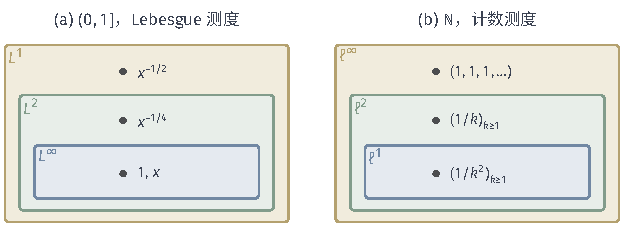
\includegraphics[width=105.7mm]{figures/02-abstract-mathematics/03-function-spaces/tikz/c1-inclusions/figure.pdf}
  \caption{两种测度下的包含方向，嵌套的框表示集合包含，点为各层之间的例子。(a)$(0,1]$上取Lebesgue测度，总质量有限：$L^\infty\subseteq L^2\subseteq L^1$，$x^{-1/4}$在$L^2$中但无界，$x^{-1/2}$可积但不平方可积。(b)$\mathbb N_+$上取计数测度：$\ell^1\subseteq\ell^2\subseteq\ell^\infty$，方向相反。}
  \label{fig:fs-inclusions}
\end{figure}

\paragraph{连续函数进入积分空间}
把一个连续函数“看作”$L^p$中的元素，实际上是一个映射。设$K$是紧度量空间，$\mu$是$K$上的有限Borel测度。连续函数有界且Borel可测，所以$\iota(f)=[f]_\mu$定义了线性映射$\iota:C(K)\to L^p(\mu)$，并且由定理~\ref{thm:fs-lp-inclusion}，
\[
 \|\iota(f)\|_p\leq\mu(K)^{1/p}\|f\|_\infty .
\]
这个映射不一定单射。若$\mu$是全支撑的，即每个非空开集的测度为正，则$f\neq g$时$\{f\neq g\}$是非空开集，测度为正，所以$\iota(f)\neq\iota(g)$。若$\mu$不是全支撑的，例如在$K=[0,1]$上令$\mu(A)$为$A\cap[0,\tfrac12]$的长度，则$f(x)=\max(0,x-\tfrac12)$是非零连续函数，而$\iota(f)=0$。所以只有核实了单射条件，才能把$C(K)$当作$L^p(\mu)$的子空间。

有限测度的假设也不能省。在$\mathbb R$上取Lebesgue测度，常数函数$1$属于$C_b(\mathbb R)$，却不属于任何$L^p$（$p<\infty$）。再取$h_n=\tfrac1n\mathbf 1_{[0,n^2]}$，有$\|h_n\|_\infty=\tfrac1n\to0$，而$\|h_n\|_2^2=\tfrac1{n^2}\cdot n^2=1$：高度在降低，支撑却在扩大，最大偏差趋于零不能推出平方积分误差趋于零。

\subsection{换测度后的元素与范数}
\label{sec:fs-change-of-measure}

同一个可测集合上换一个测度，首先改变的是“哪些差别不计”，其次才是误差的大小。设$\mu,\nu$是同一可测空间上的两个测度。若每个$\mu$零测集也是$\nu$零测集，称$\nu$关于$\mu$\term{绝对连续}（absolutely continuous），记作$\nu\ll\mu$；若两个方向都成立，称它们为\term{等价测度}（equivalent measures）。这些概念见第~\ref{sec:measure-absolute-continuity}节，Radon--Nikodym定理见第~\ref{sec:density-radon-nikodym}节。

\paragraph{零集关系与等价类}
若$\nu\ll\mu$，则$\mu$下几乎处处相等的两个函数在$\nu$下也几乎处处相等，所以$[f]_\mu\mapsto[f]_\nu$不依赖代表，是可测函数等价类之间良定义的线性映射。但它不一定是单射，也不一定保持可积性。

以$[0,1]$上的Lebesgue测度$\mu$与$d\nu=w\,d\mu$为例，其中$w\geq0$可测。由第~\ref{sec:density-weighted-measure}节，$\nu(A)=\int_Aw\,d\mu$是测度且$\nu\ll\mu$，并且$\int h\,d\nu=\int hw\,d\mu$对非负可测$h$成立。若$w=2\cdot\mathbf 1_{[0,1/2]}$，则$f=\mathbf 1_{(1/2,1]}$在$\mu$下不是零元素，在$\nu$下却是：新测度把原来不同的元素合并了。若$w>0$几乎处处，则$\mu\ll\nu$也成立，两个测度识别相同的零差别。

\paragraph{密度界与范数换算}
零集相同还不能保证误差可以互相控制，这需要密度的上下界。对$1\leq p<\infty$与可测函数$h$，
\[
 \|h\|_{L^p(\nu)}^p=\int_X|h|^p\,w\,d\mu .
\]
若$w\leq C$几乎处处，则$\|h\|_{L^p(\nu)}\leq C^{1/p}\|h\|_{L^p(\mu)}$，所以$L^p(\mu)$的成员都在$L^p(\nu)$中，$\mu$下的收敛推出$\nu$下的收敛。若还有$w\geq c>0$几乎处处，则$c^{1/p}\|h\|_{L^p(\mu)}\leq\|h\|_{L^p(\nu)}$，两个空间的成员相同，范数等价。

没有正下界时，反方向可能失败。取$w(x)=2x$与$f(x)=x^{-1/2}$，则
\[
 \int_0^1|f|^2\,d\mu=\int_0^1\frac{dx}{x}=\infty,\qquad \int_0^1|f|^2\,d\nu=\int_0^1\frac{1}{x}\cdot2x\,dx=2 .
\]
图~\ref{fig:fs-change-of-measure}显示了原因：$|f|^2=1/x$在$0$附近的面积无界，而权重$w=2x$恰好在那里趋于零，乘积是常数$2$。所以$f\in L^2(\nu)$但$f\notin L^2(\mu)$，尽管两个测度的零集相同。这里的$w\leq2$只给出$\|h\|_{L^2(\nu)}\leq\sqrt2\|h\|_{L^2(\mu)}$这一个方向。

\begin{figure}[!htb]
  \centering
  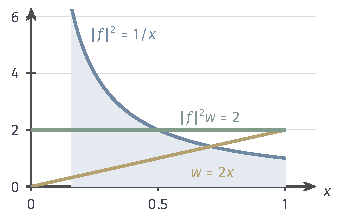
\includegraphics[width=58.1mm]{figures/02-abstract-mathematics/03-function-spaces/tikz/c1-change-of-measure/figure.pdf}
  \caption{换测度后的平方积分。$(0,1]$上$f(x)=x^{-1/2}$，$|f|^2=1/x$（蓝），其下方面积在$0$附近无界（阴影只画到$x=0.16$）；密度$w=2x$（黄）在$0$处趋于零，乘积$|f|^2w=2$（绿）的积分为$2$。所以$f\in L^2(w\,dx)$而$f\notin L^2(dx)$。}
  \label{fig:fs-change-of-measure}
\end{figure}

\paragraph{本质上界的换测度}
$L^\infty$只依赖零集，不需要密度界。若$\nu\ll\mu$，则$\{|f|>M\}$为$\mu$零测时也为$\nu$零测，所以$\|f\|_{L^\infty(\nu)}\leq\|f\|_{L^\infty(\mu)}$；若两个测度等价，本质上确界相同。把有限$p$的估计$C^{1/p}$令$p\to\infty$也能猜出这个结论，但它的成立靠的是零集关系，不是积分公式的极限。

\subsection{稠密子集与可分性}
\label{sec:fs-density-separability}

一般的$L^p$成员可能很不规则，计算和证明时常希望先对简单的函数验证，再推广到全空间。这要求简单函数能以任意精度逼近一般成员。度量空间中，若$D$的闭包是整个空间，称$D$\term{稠密}（dense）（定义~\ref{def:metric-separable}）。

\paragraph{简单函数的稠密性}
取值只有有限多个的可测函数称为简单函数。下面的定理说明，有限$p$的$L^p$中，支撑测度有限的简单函数已经足够。

\begin{theorem}[简单函数在$L^p$中稠密]
\label{thm:fs-simple-dense}
设$1\leq p<\infty$。形如$s=\sum_{i=1}^ka_i\mathbf 1_{A_i}$、其中$\mu(A_i)<\infty$的简单函数在$L^p(\mu)$中稠密。
\end{theorem}

\begin{proof}
先设$f\geq0$。取标准的二进逼近$s_n=\min\bigl(n,\,2^{-n}\lfloor2^nf\rfloor\bigr)$，它是简单函数，满足$0\leq s_n\leq f$且$s_n\uparrow f$逐点成立。于是$|f-s_n|^p\leq f^p$，后者可积，由控制收敛定理$\|f-s_n\|_p\to0$。每个$s_n$的非零取值至少为$2^{-n}$，而$\mu(\{s_n\geq2^{-n}\})\leq\mu(\{f\geq2^{-n}\})\leq2^{np}\|f\|_p^p<\infty$（最后一步是Chebyshev不等式），所以$s_n$的支撑测度有限。一般的$f$写成$f=f^+-f^-$，分别逼近后相减，由三角不等式即得。
\end{proof}

图~\ref{fig:fs-step-density}画出了$f(x)=\sin(\pi x)$的二进逼近。层高每减半一次，阶梯就更贴近曲线：$0\leq f-s_n<2^{-n}$，$n=2$时$L^2$误差约为$0.164$，$n=3$时约为$0.079$。这里$f$有界，所以截断$\min(n,\cdot)$不起作用；对无界的$f$，截断保证每个$s_n$只取有限多个值。

\begin{figure}[!htb]
  \centering
  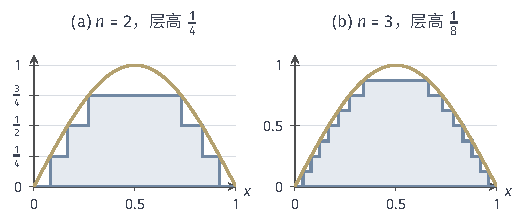
\includegraphics[width=88.7mm]{figures/02-abstract-mathematics/03-function-spaces/tikz/c1-step-density/figure.pdf}
  \caption{用二进简单函数逼近$f(x)=\sin(\pi x)$。$s_n=2^{-n}\lfloor2^nf\rfloor$在$f$落入$[k2^{-n},(k+1)2^{-n})$的位置取值$k2^{-n}$；(a)$n=2$，(b)$n=3$。逐点误差小于$2^{-n}$，$L^2([0,1])$误差约为$0.164$与$0.079$。}
  \label{fig:fs-step-density}
\end{figure}

\paragraph{连续紧支撑函数的稠密性}
在欧氏空间上，还可以用连续函数逼近。记$C_c(\Omega)$为开集$\Omega\subseteq\mathbb R^d$上支撑为紧集的连续函数。

\begin{theorem}[连续紧支撑函数在$L^p(\Omega)$中稠密]
\label{thm:fs-cc-dense}
设$\Omega\subseteq\mathbb R^d$为开集，取Lebesgue测度，$1\leq p<\infty$。则$C_c(\Omega)$在$L^p(\Omega)$中稠密。
\end{theorem}

\begin{proof}
由定理~\ref{thm:fs-simple-dense}和三角不等式，只需逼近有限测度可测集$A\subseteq\Omega$的示性函数。由Lebesgue测度的正则性，对$\varepsilon>0$存在紧集$K$与开集$U$，使$K\subseteq A\subseteq U\subseteq\Omega$且$\lambda(U\setminus K)<\varepsilon$；缩小$U$还可使其闭包是$\Omega$中的紧集。令
\[
 \varphi(x)=\frac{\operatorname{dist}(x,U^c)}{\operatorname{dist}(x,U^c)+\operatorname{dist}(x,K)} .
\]
分母处处为正，$\varphi$连续，在$K$上等于$1$、在$U$外等于$0$、取值在$[0,1]$中，所以$\varphi\in C_c(\Omega)$。$\mathbf 1_A-\varphi$只在$U\setminus K$上非零且绝对值不超过$1$，故$\|\mathbf 1_A-\varphi\|_p^p\leq\lambda(U\setminus K)<\varepsilon$。
\end{proof}

取$\Omega=\mathbb R^d$，定理~\ref{thm:fs-cc-dense}特别给出：$C_c(\mathbb R^d)$在$L^p(\mathbb R^d)$（$1\leq p<\infty$）中稠密。

同样的“先逼近示性函数、再用距离函数构造连续过渡”的论证不依赖欧氏结构，只需测度能被闭集和开集从内外逼近。度量空间上的有限Borel测度具有这种正则性：对每个Borel集$A$与$\varepsilon>0$，存在闭集$F$与开集$U$，使$F\subseteq A\subseteq U$且$\mu(U\setminus F)<\varepsilon$。由此得到紧度量空间上的版本。

\begin{theorem}[紧度量空间上连续函数的稠密性]
\label{thm:fs-continuous-dense-compact}
设$K$为紧度量空间，$\mu$为$K$上的有限Borel测度，$1\leq p<\infty$。则$\{[f]_\mu:f\in C(K)\}$在$L^p(\mu)$中稠密。
\end{theorem}

\begin{proof}
由定理~\ref{thm:fs-simple-dense}，只需逼近Borel集$A$的示性函数。按上面的正则性取闭集$F\subseteq A\subseteq U$（$U$开，$\mu(U\setminus F)<\varepsilon$），定义与定理~\ref{thm:fs-cc-dense}证明中相同的$\varphi$，只把$K$换成$F$。$F$闭、$U^c$闭且二者不交，所以分母处处为正，$\varphi$连续，在$F$上为$1$、在$U$外为$0$，于是$\|\mathbf 1_A-\varphi\|_p^p\leq\mu(U\setminus F)<\varepsilon$。$U=K$或$F=\varnothing$时分别取$\varphi\equiv1$或$\varphi\equiv0$即可。
\end{proof}

\paragraph{区间阶梯函数的稠密性}
在$L^2(0,1)$中，比连续函数更简单的区间阶梯函数也已足够。所谓区间阶梯函数，是有限个区间示性函数的线性组合。给定$f\in L^2(0,1)$与$\varepsilon>0$，由定理~\ref{thm:fs-cc-dense}取连续函数$g$使$\|f-g\|_2<\varepsilon$；$g$在$[0,1]$上一致连续（定理~\ref{thm:metric-compact-uniform}），取$m$足够大，使每个长为$1/m$的区间上$g$的振幅小于$\varepsilon$，令$s$在$[(j-1)/m,j/m)$上取常数$g(j/m)$，则$\|g-s\|_\infty\leq\varepsilon$，从而$\|g-s\|_2\leq\varepsilon$。合起来$\|f-s\|_2<2\varepsilon$。所以区间阶梯函数在$L^2(0,1)$中稠密；同样的论证对任意有限$p$成立。

这些结论回答了斜坡例子留下的问题。$C([-1,1])$在$L^2([-1,1])$中稠密，而$L^2([-1,1])$完备，所以$L^2([-1,1])$正是$(C([-1,1]),\|\cdot\|_2)$的完备化：第~\ref{sec:fs-banach}小节抽象构造出来的“新元素”，在这里被识别为平方可积函数的等价类。用光滑函数逼近需要卷积平滑，留到第~\ref{sec:sob-mollification}小节。

\paragraph{可分性}
稠密子集可以很大。若一个空间有可数的稠密子集，称它\term{可分}（separable）（定义~\ref{def:metric-separable}）。可分空间中的每个元素都能用可数多个“标准对象”中的某些去逼近，这在构造可数正交基、对角线抽取子列时都要用到。

$C([a,b])$可分。Weierstrass逼近定理断言多项式在$(C([a,b]),\|\cdot\|_\infty)$中稠密，证明见第~\ref{sec:apx-polynomial}小节；把多项式的系数换成有理数，误差可以任意小，而有理系数多项式只有可数多个。$\ell^p$（$1\leq p<\infty$）可分：只有有限个非零项且各项为有理数的数列可数，截断尾部和把各项换成有理数都只产生任意小的误差。$L^p(\Omega)$（$1\leq p<\infty$）也可分：由定理~\ref{thm:fs-cc-dense}，可以先用连续紧支撑函数逼近，再在其支撑上用有理系数多项式一致逼近，并乘以有理顶点方体的示性函数（其细节与上面的证明类似，这里从略）。

可数稠密子集与有限维基是两回事。$C([a,b])$中的有理系数多项式可数且稠密，但$e^x$不是其中任何一个的有限线性组合；可分只说明每个元素是可数集合中元素的极限，不说明它能用有限多个方向精确表示。

可分性也不是所有函数空间的共同性质。在$L^\infty([0,1])$中取$f_t=\mathbf 1_{[0,t]}$，$t\in[0,1]$。对$s<t$，$f_t-f_s=\mathbf 1_{(s,t]}$在正测度集上等于$1$，所以$\|f_t-f_s\|_\infty=1$。以每个$f_t$为中心、半径$\tfrac12$的开球两两不交，共有不可数个；若$D$稠密，每个球中至少有$D$的一个元素，且这些元素各不相同，所以$D$不可数。故$L^\infty([0,1])$不可分。同样的论证用于$0$--$1$数列，说明$\ell^\infty$不可分。

\subsection{收敛方式与误差传递}
\label{sec:fs-convergence-modes}

函数列可以在多种意义下收敛。本小节先说明怎样用范数不等式把一种收敛传给另一种，再用三个对照序列标出不能推出的边界。

\paragraph{用范数不等式传递收敛}
设同一线性空间上有两个范数，且存在与序号无关的常数$C$，使$\|h\|_A\leq C\|h\|_B$对所有$h$成立。对$h=f_n-f$使用这个不等式，$\|f_n-f\|_B\to0$即推出$\|f_n-f\|_A\to0$。若两个方向都有这样的常数，两种收敛等价。关键在于常数不随$n$变化，并且两个范数作用于同一列函数、同一个候选极限。

由定理~\ref{thm:fs-lp-inclusion}，在有限测度空间上，$L^q$收敛推出$L^p$收敛（$p<q$），一致收敛推出每个$L^p$收敛。$\mathbb R$上$h_n=\tfrac1n\mathbf 1_{[0,n^2]}$的例子说明，测度无限时后一结论失效。

\paragraph{三个对照序列}
图~\ref{fig:fs-convergence-modes}和表~\ref{tab:fs-convergence-modes}对照了$[0,1]$上Lebesgue测度下的三个序列。

\begin{figure}[!htb]
  \centering
  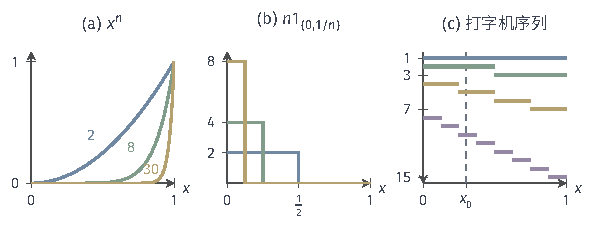
\includegraphics[width=100.4mm]{figures/02-abstract-mathematics/03-function-spaces/tikz/c1-convergence-modes/figure.pdf}
  \caption{三种收敛方式的反例。(a)$x^n$，$n=2,8,30$：逐点趋于端点处为$1$、其余为$0$的函数，$L^p$范数趋于零，最大偏差恒为$1$。(b)窄尖峰$n\mathbf 1_{(0,1/n)}$，$n=2,4,8$：每一点最终为零，积分却恒为$1$。(c)打字机序列的前$15$项，第$k$层把$[0,1)$等分为$2^k$段，依次取各段的示性函数；纵轴为项号，横条为支撑。竖虚线$x=x_0$在每一层恰好穿过一个横条。}
  \label{fig:fs-convergence-modes}
\end{figure}

\begin{table}[!htb]
  \centering
  \begin{tabular}{@{}lccc@{}}
    \toprule
    序列 & 逐点收敛到$0$ & $L^1$收敛到$0$ & 一致收敛到$0$ \\
    \midrule
    $x^n$ & 除$x=1$外 & 是 & 否 \\
    $n\mathbf 1_{(0,1/n)}$ & 是（处处） & 否 & 否 \\
    打字机序列 & 处处不收敛 & 是 & 否 \\
    \bottomrule
  \end{tabular}
  \caption{$[0,1]$上Lebesgue测度下三个序列的收敛性质。}
  \label{tab:fs-convergence-modes}
\end{table}

$x^n$的计算已在第~\ref{sec:fs-lp}小节完成：$\|x^n\|_p=(np+1)^{-1/p}\to0$，逐点极限在$x=1$处为$1$，但这只是一个零测点，所以作为$L^p$元素，逐点极限与零元素相同，两种说法并不矛盾。最大偏差恒为$1$，不一致收敛。

窄尖峰$g_n=n\mathbf 1_{(0,1/n)}$在每个$x$处最终为零：$x\leq0$时恒为零，$x>0$时只要$n>1/x$就有$g_n(x)=0$。但$\|g_n\|_1=1$，$\|g_n\|_2=\sqrt n\to\infty$。逐点收敛允许不同位置在不同时刻进入误差带，因而管不住越来越窄、越来越高的峰。

\begin{example}[打字机序列]
\label{ex:fs-typewriter}
对$k=0,1,2,\ldots$与$j=0,\ldots,2^k-1$，令$h_{k,j}=\mathbf 1_{[j2^{-k},(j+1)2^{-k})}$，并按$k$从小到大、同一层内按$j$从小到大排成一列：$h_{0,0},h_{1,0},h_{1,1},h_{2,0},\ldots$。第$k$层每一项的范数是$\|h_{k,j}\|_p=2^{-k/p}$，随项号增大趋于零，所以序列在每个$L^p$（$p<\infty$）中收敛到$0$。但对每个$x_0\in[0,1)$，每一层恰好有一项在$x_0$处取$1$，其余项取$0$，所以数列$(h_{k,j}(x_0))$中$0$和$1$都出现无穷多次，在任何一点都不收敛。
\end{example}

\paragraph{子列与控制条件}
打字机序列说明$L^p$收敛推不出整列的逐点收敛，但定理~\ref{thm:fs-ae-subsequence}保证可以抽出几乎处处收敛的子列。这里可以直接写出一个：子列$h_{k,0}=\mathbf 1_{[0,2^{-k})}$对每个$x>0$在$2^{-k}<x$后恒为零，所以它在$(0,1]$上逐点收敛到$0$，例外只有零测点$x=0$。

反方向，从几乎处处收敛推出$L^p$收敛需要附加条件。若$f_n\to f$几乎处处，且存在同一个$G\in L^p$使$|f_n|\leq G$几乎处处对所有$n$成立，则$|f|\leq G$，$|f_n-f|^p\leq2^pG^p$可积，由控制收敛定理$\|f_n-f\|_p\to0$。窄尖峰没有这样的控制函数：$\sup_ng_n(x)$在$x\in[\tfrac1{n+1},\tfrac1n)$上至少为$n$，大于$\tfrac1x-1$，不可积。所以“每项各自可积”不能代替“同一个可积函数控制所有项”。

\paragraph{弱收敛的预告}
还有一种收敛不要求整体误差趋于零。在$L^2(0,2\pi)$中取$u_n(x)=\sin(nx)$，有$\|u_n\|_2^2=\pi$，序列不趋于零。但对任意区间$[a,b]\subseteq[0,2\pi]$，
\[
 \int_0^{2\pi}\sin(nx)\,\mathbf 1_{[a,b]}(x)\,dx=\frac{\cos(na)-\cos(nb)}{n}\to0 :
\]
与每个固定的阶跃函数比较，$u_n$越来越接近零函数。这种“通过每个固定的连续线性读取来判断极限”的收敛称为弱收敛，它需要先建立线性泛函，正式定义见第~\ref{sec:lfo-weak-convergence}小节。它与概率测度的弱收敛（第~\ref{sec:wlim-weak-convergence}节）名字相同，但变化的对象与测试对象都不同，不能互换。

% 第1章第6节：Hilbert空间的正交结构（闭子空间的正交投影；正交系与正交基；正交展开与截断误差）。

\section{Hilbert空间的正交结构}
\label{sec:fs-orthogonal}

本节固定一个Hilbert空间$H$，例如$L^2(\mu)$或$\ell^2$，研究两个几何问题：给定一个子空间，能否从中取出离目标最近的分量；能否用一组两两正交的方向给每个元素写出坐标。有限维中的答案是熟悉的，无限维中的新问题是极限是否存在、是否留在子空间里。下一章将把这里的投影看作有界线性算子，本节只建立几何结论。

\subsection{闭子空间的正交投影}
\label{sec:fs-projection}

设$M\subseteq H$是线性子空间，$f\in H$。我们想找$M$中离$f$最近的元素，即达到
\[
 d(f,M)=\inf_{m\in M}\|f-m\|
\]
的$m$。下确界总存在，问题是它能否被$M$中的某个元素取到、取到的元素是否唯一。

\begin{theorem}[闭子空间上的正交投影]
\label{thm:fs-projection}
设$H$为Hilbert空间，$M\subseteq H$为闭线性子空间。则对每个$f\in H$，存在唯一的$m_*\in M$使$\|f-m_*\|=d(f,M)$；并且对$m\in M$，$\|f-m\|=d(f,M)$当且仅当$f-m$与$M$中每个元素正交。
\end{theorem}

\begin{proof}
记$d=d(f,M)$。证明分四步，前两步得到存在性，后两步得到正交刻画与唯一性。

第一步，极小化序列是Cauchy列。取$m_n\in M$使$\|f-m_n\|^2<d^2+1/n$。对$f-m_j$与$f-m_k$使用平行四边形恒等式，
\[
 \|m_j-m_k\|^2=2\|f-m_j\|^2+2\|f-m_k\|^2-4\Bigl\|f-\frac{m_j+m_k}{2}\Bigr\|^2 .
\]
$M$是线性子空间，中点$\tfrac{m_j+m_k}2$在$M$中，所以最后一项的范数平方至少为$d^2$。于是$\|m_j-m_k\|^2<2/j+2/k$，$(m_n)$是Cauchy列。

第二步，极限存在且留在$M$中。$H$完备，所以$m_n$收敛到某个$m_*\in H$；$M$闭，所以$m_*\in M$。由范数的连续性，$\|f-m_*\|=\lim_n\|f-m_n\|=d$。

第三步，最近点的残差与$M$正交。设$m_*$达到$d$，记$r=f-m_*$。任取$m\in M$与实数$t$，$m_*+tm\in M$，所以
\[
 \|r\|^2\leq\|r-tm\|^2=\|r\|^2-2t\langle r,m\rangle+t^2\|m\|^2 .
\]
即$t^2\|m\|^2-2t\langle r,m\rangle\geq0$对所有实数$t$成立。若$\langle r,m\rangle\neq0$，取符号与之相同的足够小的$t$会使左边为负，矛盾；故$\langle r,m\rangle=0$。复Hilbert空间中把$t$换成$t\langle m,r\rangle$即可得到同样的结论。

第四步，正交的残差给出唯一的最近点。设$m_*\in M$满足$f-m_*\perp M$。对任意$m\in M$，$m_*-m\in M$与$f-m_*$正交，由勾股恒等式
\[
 \|f-m\|^2=\|f-m_*\|^2+\|m_*-m\|^2 ,
\]
所以$\|f-m\|\geq\|f-m_*\|$，等号当且仅当$m=m_*$。结合第三步，达到$d$的元素恰好是使残差正交的元素，且只有一个。
\end{proof}

图~\ref{fig:fs-projection-geometry}是这个定理的示意。完备性和闭性在第二步中分工明确：前者保证极小化序列有极限，后者保证极限没有离开$M$。第一步用到了平行四边形恒等式，所以这个论证依赖内积；在一般的Banach空间中，最近点可能不存在，也可能不唯一。

\begin{figure}[!htb]
  \centering
  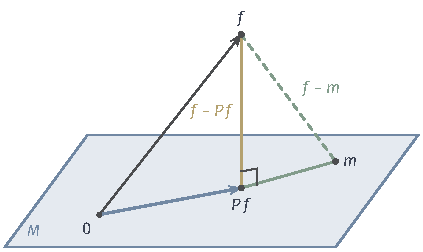
\includegraphics[width=71.7mm]{figures/02-abstract-mathematics/03-function-spaces/tikz/c1-projection-geometry/figure.pdf}
  \caption{闭子空间上的正交投影（示意）。平面代表闭子空间$M$，$Pf$是$M$中离$f$最近的点，残差$f-Pf$与$M$垂直。对$M$中任意另一点$m$，三点构成直角三角形，$\|f-m\|^2=\|f-Pf\|^2+\|Pf-m\|^2$，所以$m$离$f$更远。}
  \label{fig:fs-projection-geometry}
\end{figure}

\paragraph{正交分解与投影的性质}
把定理中的$m_*$记为$P_Mf$，称为$f$在$M$上的\term{正交投影}（orthogonal projection）。记$M^\perp=\{g\in H:\langle g,m\rangle=0\ \text{对所有}\ m\in M\}$为$M$的\term{正交补}（orthogonal complement）。它是闭线性子空间：线性由内积的线性得到，闭性由内积的连续性（Cauchy--Schwarz不等式）得到。定理给出分解
\[
 f=P_Mf+(f-P_Mf),\qquad P_Mf\in M,\quad f-P_Mf\in M^\perp ,
\]
而且这种分解唯一：若$f=m+g=m'+g'$，则$m-m'=g'-g$同时属于$M$与$M^\perp$，与自身正交，只能为零。因此$H=M\oplus M^\perp$。

由正交刻画还可以读出$P_M$的三条性质。线性：$af+bg-(aP_Mf+bP_Mg)=a(f-P_Mf)+b(g-P_Mg)\perp M$，所以$P_M(af+bg)=aP_Mf+bP_Mg$。幂等：$m\in M$时$m$自己就是最近点，$P_M(P_Mf)=P_Mf$。不扩张：由勾股恒等式$\|f\|^2=\|P_Mf\|^2+\|f-P_Mf\|^2$，得$\|P_Mf\|\leq\|f\|$。第~\ref{sec:lfo-self-adjoint}小节将从算子的角度刻画这类映射。

最简单的例子是向常数投影。在$L^2([-1,1])$中取$M=\operatorname{span}\{1\}$，正交条件$\int_{-1}^1(f-c)\,dx=0$给出$c=\tfrac12\int_{-1}^1f\,dx$，即投影是平均值。对$f=x^2$，$P_Mf=\tfrac13$，残差$x^2-\tfrac13$与$1$正交，距离平方为
\[
 \int_{-1}^1\Bigl(x^2-\frac13\Bigr)^2dx=\frac25-\frac49+\frac29=\frac{8}{45} .
\]
这个数在第~\ref{sec:fs-orthonormal-bases}小节的Gram--Schmidt计算中还会出现。

\paragraph{闭性缺失时最近点可能不存在}
定理中的闭性不能去掉。在$H=L^2([-1,1])$中，令$M$为具有连续代表的等价类组成的子空间，它是线性子空间，但由定理~\ref{thm:fs-cc-dense}它在$H$中稠密而不等于$H$，所以不闭。取$f=\operatorname{sgn}$，斜坡给出$\|f-g_n\|_2^2=\tfrac{2}{3n}\to0$，于是$d(f,M)=0$。若下确界被某个$m\in M$取到，则$\|f-m\|_2=0$，$\operatorname{sgn}$与一个连续函数几乎处处相等；而第~\ref{sec:fs-banach}小节已经证明这不可能。所以最近点不存在：每个连续函数都可以再改进，却没有最好的那一个。

本节只处理线性子空间。向一般闭凸集投影时，最近点仍然存在且唯一，但正交条件要换成变分不等式，这与约束优化一起讨论，可参考\BookChapterRef{chap:constrained-optimization}{卷三“有约束优化的求解”章}。

\subsection{正交系与正交基}
\label{sec:fs-orthonormal-bases}

有限维空间中，投影可以用标准正交基的坐标直接写出。现在考察无限多个正交方向。

\begin{definition}[正交归一系]
\label{def:fs-orthonormal}
Hilbert空间$H$中的序列（有限或可数）$(e_j)$称为\term{正交归一系}（orthonormal system），若$\langle e_j,e_k\rangle=\delta_{j,k}$，即两两正交且各自范数为$1$。
\end{definition}

\paragraph{有限个方向上的投影与Bessel不等式}
设$e_1,\ldots,e_m$正交归一，$M_m=\operatorname{span}\{e_1,\ldots,e_m\}$。有限维子空间是闭的（有限维赋范空间完备），所以定理~\ref{thm:fs-projection}适用。记$c_j=\langle e_j,f\rangle$，则
\begin{equation}
 P_{M_m}f=\sum_{j=1}^mc_je_j .
 \label{eq:fs-finite-projection}
\end{equation}
验证只需检查残差：$\langle e_k,f-\sum_jc_je_j\rangle=c_k-c_k=0$对每个$k\leq m$成立，所以残差与$M_m$正交。由勾股恒等式与正交归一性，
\begin{equation}
 \Bigl\|f-\sum_{j=1}^mc_je_j\Bigr\|^2=\|f\|^2-\sum_{j=1}^m|c_j|^2 .
 \label{eq:fs-bessel-error}
\end{equation}

\begin{theorem}[Bessel不等式]
\label{thm:fs-bessel}
设$(e_j)_{j\geq1}$为$H$中的正交归一系，$f\in H$。则$\sum_{j\geq1}|\langle e_j,f\rangle|^2\leq\|f\|^2$。
\end{theorem}

\begin{proof}
由式~\eqref{eq:fs-bessel-error}，左边每个部分和都不超过$\|f\|^2$。非负项级数的部分和有界，级数收敛且和不超过这个界。
\end{proof}

Bessel不等式说明系数平方可和，于是$c_j\to0$：任何元素在越来越靠后的正交方向上的分量都越来越小。

\paragraph{Gram--Schmidt与可数正交基的来源}
正交归一系可以从任意线性无关的序列造出来。设$u_1,u_2,\ldots$线性无关，依次令
\[
 v_k=u_k-\sum_{j<k}\langle e_j,u_k\rangle e_j,\qquad e_k=\frac{v_k}{\|v_k\|} .
\]
$v_k$是$u_k$减去它在$\operatorname{span}\{e_1,\ldots,e_{k-1}\}$上的投影，与之前的方向正交；线性无关保证$v_k\neq0$。归纳可知$\operatorname{span}\{e_1,\ldots,e_k\}=\operatorname{span}\{u_1,\ldots,u_k\}$对每个$k$成立。这就是有限维中的\term{Gram--Schmidt正交化}（Gram--Schmidt orthogonalization），只是现在可以无限地进行下去。

在$L^2([-1,1])$中对$1,x,x^2,x^3$执行这一过程。$e_0=1/\sqrt2$。$x$与$1$正交，$\|x\|^2=\tfrac23$，所以$e_1=\sqrt{3/2}\,x$。对$x^2$，$\langle e_0,x^2\rangle=\tfrac{\sqrt2}3$，$\langle e_1,x^2\rangle=0$，于是$v_2=x^2-\tfrac13$，这正是上一小节向常数投影的残差，$\|v_2\|^2=\tfrac8{45}$，故
\[
 e_2=\sqrt{\tfrac{45}{8}}\Bigl(x^2-\frac13\Bigr)=\sqrt{\tfrac58}\,(3x^2-1).
\]
对$x^3$，它与$e_0,e_2$正交，$\langle e_1,x^3\rangle e_1=\tfrac32\cdot\tfrac25x=\tfrac35x$，于是$v_3=x^3-\tfrac35x$，$\|v_3\|^2=\tfrac27-\tfrac{12}{25}+\tfrac{6}{25}=\tfrac{8}{175}$，故$e_3=\sqrt{7/8}\,(5x^3-3x)$。这些就是归一化的Legendre多项式。图~\ref{fig:fs-legendre-gram-schmidt}对照了正交化前后的函数：(a)中$x^2$与$1$、$x^3$与$x$在大部分区间上走向相近，彼此远不正交；(b)中每个$e_k$恰好比前一个多一次变号。

\begin{figure}[!htb]
  \centering
  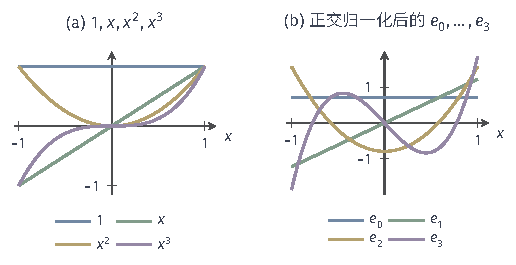
\includegraphics[width=87.3mm]{figures/02-abstract-mathematics/03-function-spaces/tikz/c1-legendre-gram-schmidt/figure.pdf}
  \caption{在$L^2([-1,1])$中对单项式做Gram--Schmidt正交化。(a)$1,x,x^2,x^3$，例如$\langle1,x^2\rangle=\tfrac23\neq0$；(b)得到的$e_0=1/\sqrt2$，$e_1=\sqrt{3/2}\,x$，$e_2=\sqrt{5/8}\,(3x^2-1)$，$e_3=\sqrt{7/8}\,(5x^3-3x)$，两两正交且范数为$1$，$e_k$在$(-1,1)$内恰有$k$个零点。}
  \label{fig:fs-legendre-gram-schmidt}
\end{figure}

同一过程解释了可分Hilbert空间中可数正交归一系的来源。设$H$可分，取可数稠密子集$\{u_k\}$，依次删去能由前面元素线性表出的项，再做Gram--Schmidt，得到正交归一系$(e_j)$，其张成与$\{u_k\}$的张成相同，因而在$H$中稠密。

\paragraph{正交系的完备性}
上面得到的正交系有一个关键性质：它的有限线性组合在$H$中稠密。

\begin{definition}[完备正交系]
\label{def:fs-complete-system}
若正交归一系$(e_j)$的闭线性张成$\overline{\operatorname{span}}\{e_j\}$等于$H$，称它为$H$的\term{完备正交系}（complete orthonormal system），也称\term{标准正交基}（orthonormal basis）。
\end{definition}

这里的“完备”与空间的完备是两个不同的概念：前者说正交系的方向够用，后者说Cauchy列有极限。完备正交系可以用正交性来检验：$(e_j)$完备当且仅当与所有$e_j$都正交的元素只有零。若$(e_j)$完备而$g\perp e_j$对所有$j$成立，则$g$与$\operatorname{span}\{e_j\}$正交，由内积的连续性也与其闭包$H$正交，特别地$\langle g,g\rangle=0$。反之，若闭张成$M\neq H$，取$f\notin M$，由定理~\ref{thm:fs-projection}，$f-P_Mf$是非零元素且与每个$e_j$正交。

\begin{example}[偶方向遗漏奇函数]
\label{ex:fs-even-subspace}
在$L^2([-1,1])$中，偶次的归一化Legendre多项式$e_0,e_2,e_4,\ldots$组成一个无限的正交归一系。但$x$是奇函数，与每个偶函数正交（乘积为奇函数，积分为零），而$x\neq0$，所以这个系不完备。方向有无穷多个，正交性也成立，却仍然遗漏了整个奇函数子空间。

设$E$为几乎处处满足$f(-x)=f(x)$的元素组成的子空间，它是闭的（$L^2$收敛列有几乎处处收敛子列，定理~\ref{thm:fs-ae-subsequence}，极限保持偶性）。任意$f$可以写成$f=\tfrac{f(x)+f(-x)}{2}+\tfrac{f(x)-f(-x)}{2}$，前者是偶函数，后者是奇函数，与$E$正交，所以由定理~\ref{thm:fs-projection}，$P_Ef(x)=\tfrac{f(x)+f(-x)}2$。取$f=e^x$，得$P_Ef=\cosh x$，残差$\sinh x$，见图~\ref{fig:fs-even-odd-projection}；距离平方为$\int_{-1}^1\sinh^2x\,dx=\tfrac{\sinh2}{2}-1\approx0.813$，无论加入多少偶方向都无法减小。
\end{example}

\begin{figure}[!htb]
  \centering
  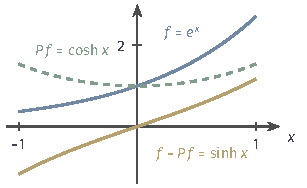
\includegraphics[width=51.9mm]{figures/02-abstract-mathematics/03-function-spaces/tikz/c1-even-odd-projection/figure.pdf}
  \caption{向偶函数子空间的正交投影。$[-1,1]$上$f(x)=e^x$（蓝），投影$Pf=\cosh x$（绿，虚线）为其偶部，残差$f-Pf=\sinh x$（黄）为奇函数，与每个偶函数正交。只用偶方向展开$e^x$时，误差始终至少为$\|\sinh\|_2\approx0.90$。}
  \label{fig:fs-even-odd-projection}
\end{figure}

\subsection{正交展开与截断误差}
\label{sec:fs-orthogonal-expansion}

有了正交归一系，就可以考察无穷级数$\sum_jc_je_j$：它是否收敛，收敛到什么，截断后误差多大。

\begin{theorem}[正交展开与Parseval等式]
\label{thm:fs-parseval}
设$(e_j)_{j\geq1}$为Hilbert空间$H$中的正交归一系，$M=\overline{\operatorname{span}}\{e_j\}$，$f\in H$，$c_j=\langle e_j,f\rangle$。则级数$\sum_jc_je_j$依范数收敛，其和为$P_Mf$。特别地，若$(e_j)$完备，则
\[
 f=\sum_{j=1}^\infty c_je_j\quad(\text{依范数}),\qquad \|f\|^2=\sum_{j=1}^\infty|c_j|^2 .
\]
后一个等式称为\term{Parseval等式}（Parseval identity）。
\end{theorem}

\begin{proof}
记部分和$s_n=\sum_{j\leq n}c_je_j$。对$n>m$，由正交归一性$\|s_n-s_m\|^2=\sum_{m<j\leq n}|c_j|^2$，由Bessel不等式这是收敛级数的一段，所以$(s_n)$是Cauchy列。$H$完备，$s_n$收敛到某个$s$；每个$s_n\in M$而$M$闭，所以$s\in M$。

再验证$f-s\perp M$。对固定的$k$与$n\geq k$，$\langle e_k,f-s_n\rangle=c_k-c_k=0$；令$n\to\infty$，由内积的连续性得$\langle e_k,f-s\rangle=0$。于是$f-s$与$\operatorname{span}\{e_j\}$正交，进而与其闭包$M$正交。由定理~\ref{thm:fs-projection}的正交刻画，$s=P_Mf$。

若$(e_j)$完备，则$M=H$，$P_Mf=f$。在式~\eqref{eq:fs-bessel-error}中令$m\to\infty$，左边趋于$0$，即得Parseval等式。
\end{proof}

对不完备的正交系，展开只恢复$f$在闭张成上的投影，正交补中的分量永远丢失；示例~\ref{ex:fs-even-subspace}中只用偶次Legendre多项式展开$e^x$，奇部$\sinh x$与每个方向都正交，得到的级数和与$e^x$的距离至少为$\|\sinh\|_2$。Bessel不等式与Parseval等式之间的差距，正是这部分丢失的分量。

\paragraph{Legendre多项式的完备性}
判断一个具体的正交系是否完备，需要稠密性论证。对Legendre多项式，三步就够了。由Weierstrass逼近定理，多项式在$(C([-1,1]),\|\cdot\|_\infty)$中稠密；由$\|h\|_2\leq\sqrt2\|h\|_\infty$，一致逼近也是$L^2$逼近；再由定理~\ref{thm:fs-cc-dense}，连续函数在$L^2([-1,1])$中稠密。所以多项式在$L^2([-1,1])$中稠密，而Legendre多项式的张成就是全体多项式，它们组成$L^2([-1,1])$的完备正交系。三角函数系$\{e^{ikx}\}$在$L^2(-\pi,\pi)$中的完备性及傅里叶分析，可参考\BookChapterRef{chap:signal-analysis}{卷三“信号”章}。

\paragraph{截断误差与系数衰减}
固定完备正交系与目标$f$，只改变保留的项数$m$。由式~\eqref{eq:fs-bessel-error}与Parseval等式，
\begin{equation}
 \|f-s_m\|^2=\sum_{j>m}|c_j|^2 ,
 \label{eq:fs-truncation-tail}
\end{equation}
截断误差就是系数平方的尾和。每个$s_m$是$f$在前$m$个方向张成的子空间上的投影，所以在这个子空间内是最好的；但它并没有与其他同样规模的表示比较过，选什么方向是第~\ref{chap:function-approximation}章的问题。

用Legendre多项式展开$\operatorname{sgn}$可以具体看到这些量。$\operatorname{sgn}$是奇函数，只有奇次系数非零；按系数公式精确计算，前几个系数平方为$c_1^2=\tfrac32$，$c_3^2=\tfrac{7}{32}$，$c_5^2=\tfrac{11}{128}$，对应的截断误差$2-\sum_{j\leq m}c_j^2$在$m=1,5,15$时约为$0.500$、$0.195$、$0.077$。图~\ref{fig:fs-legendre-truncation}(a)画出了部分和，(b)把它与$|x|$的展开对照：$|x|$连续，只在$0$处有折角，截断误差下降得快得多，$m=2$时已约为$0.0104$，$m=40$时约为$6\times10^{-6}$；$\operatorname{sgn}$有跳跃，$m=41$时误差仍约为$0.030$。这里只是两个例子的观察；系数衰减与函数光滑性之间的一般关系属于第~\ref{chap:function-approximation}章。

\begin{figure}[!htb]
  \centering
  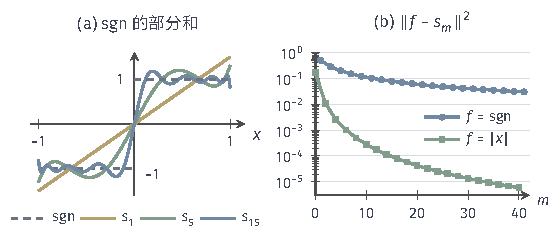
\includegraphics[width=94.9mm]{figures/02-abstract-mathematics/03-function-spaces/tikz/c1-legendre-truncation/figure.pdf}
  \caption{Legendre展开的截断。(a)$\operatorname{sgn}$（虚线）与部分和$s_1,s_5,s_{15}$，其中$s_1=\tfrac32x$；部分和是多项式，在跳跃点附近来回振荡。(b)截断误差$\|f-s_m\|_2^2$（对数纵轴）：$\operatorname{sgn}$取奇数$m$，$|x|$取偶数$m$。两条曲线都单调趋于零，有跳跃的$\operatorname{sgn}$下降慢得多。数值由精确有理运算得到。}
  \label{fig:fs-legendre-truncation}
\end{figure}

\paragraph{从范数收敛到点值收敛}
式~\eqref{eq:fs-truncation-tail}只控制$L^2$误差。图~\ref{fig:fs-legendre-truncation}(a)中的部分和都是连续函数；若它们一致收敛，极限必然连续（定理~\ref{thm:fs-continuous-complete}），而$\operatorname{sgn}$在$0$处跳跃，所以$s_m$不一致收敛到$\operatorname{sgn}$，尽管$L^2$误差趋于零。要从范数收敛得到某点处函数值的收敛，需要“该点的值受范数控制”这样的读取界；$L^2$本身不提供这种界，第~\ref{sec:lfo-point-evaluation}小节将专门讨论这个问题。

% 第1章第7节：本章小结。

\section{本章小结}
\label{sec:fs-summary}

章首的问题是：当表示规模不断变化时，怎样直接比较函数、谈论极限和正交分量。本章的回答可以归结为四个依次进行的选择：选定函数集合，确定什么算作同一个元素，规定误差，检查极限是否留在集合中。

第一个选择决定线性运算是否封闭：连续函数、多项式和固定函数的张成是线性空间，参数化的非线性族一般不是；一维输入也可以产生无限维的函数空间。第二个选择决定元素的身份：用积分衡量误差时，只在零测集上不同的函数必须看成同一个元素，代价是等价类一般没有确定的点值。第三个选择是范数，它让误差满足正定、齐次和三角不等式，从而接入度量空间的全部工具。第四个选择是完备性检查，它同时依赖集合和范数：同一个$C([-1,1])$在一致范数下完备，在平方积分范数下不完备，斜坡逼近阶跃的例子说明了二者的差别，而$L^2([-1,1])$正是后者的完备化。

三类空间的结构可以这样对照。连续函数空间$C(K)$的元素是普通函数，一致范数控制每一点，完备性来自一致收敛保持连续。$L^p(\mu)$的元素是等价类，范数累计整体偏差，Hölder与Minkowski不等式保证范数公理，完备性靠抽子列与Fatou引理（有限$p$）或合并零测例外集（$p=\infty$）得到。数列空间$\ell^p$是计数测度下的$L^p$，等价类退化为数列本身。比较这些空间时，要分清三种保证：同一个函数集合不保证相同的收敛；相同的零集保证换测度后元素的识别一致，却不保证范数可比；只有与序号无关的范数不等式才能传递收敛。三个对照序列$x^n$、窄尖峰和打字机序列标出了一致、$L^p$与逐点收敛之间不能推出的方向，子列定理与控制收敛则给出了在附加条件下可以推出的部分。

Hilbert空间在完备性之外还有内积。闭子空间上的正交投影存在且唯一，由残差正交刻画，并给出分解$H=M\oplus M^\perp$；闭性缺失时最近点可能不存在。正交归一系给出坐标：Bessel不等式对任何正交系成立，Parseval等式只对完备正交系成立，截断误差等于系数平方的尾和。但$L^2$意义下的展开收敛并不推出逐点或一致收敛。

本章把函数当作空间中的点。接下来的问题是作用在这些点上的映射：哪些线性映射能稳定地变换函数，标量读取能否统一地表示，投影作为映射有哪些性质，以及当整体误差不趋于零时，能否通过所有连续线性读取来判断极限。这些问题由第~\ref{chap:linear-functionals-operators}章的线性算子、线性泛函、对偶与弱收敛处理。


\chapter{线性泛函与线性算子}
\label{chap:linear-functionals-operators}

设想区间$[0,1]$上记录到一条信号$f$。拿到它以后，常做的事情有三类：把它平滑成局部平均，对它求导看变化率，或者从中读出一个数，例如某一点的值、某一段的平均或与某个模板的相关程度。每一种做法都是一个映射，输入是函数，输出是另一个函数或一个标量。第~\ref{chap:function-spaces}章已经说明怎样度量两个函数之间的误差；现在要问的是：输入带有小误差时，这些映射的输出误差能否统一控制？一个读数规则能否写成与某个固定函数的比较？一列函数在范数下不收敛时，能否用全部读数判断它的极限？反过来，由输出恢复输入何时可行、何时稳定？

第~\ref{sec:lfo-operators}节把矩阵作用推广到函数空间，先确定输入空间、输出空间和定义域，再用算子范数统一控制误差传递，并区分两种算子列的收敛。标量输出是最常用的特殊情形：第~\ref{sec:lfo-functional-representation}节研究单个读数规则何时有良定义、何时连续，以及在Hilbert空间中怎样表示为一个方向；第~\ref{sec:lfo-dual}节把同一空间上的全部连续读数组成对偶空间，借延拓定理说明它们足以区分不同元素，并在积分空间和连续函数空间中写出它们的具体形式。

有了全部读数，第~\ref{sec:lfo-weak}节改用“每个固定读数都收敛”来观察函数列，得到弱收敛；这里需要一致有界原理把逐点的控制转为统一的控制，并回答有界序列何时能抽出弱收敛子列。第~\ref{sec:lfo-adjoint}节回到Hilbert空间之间的一般算子，用读数的表示构造伴随，借它说明哪些输入方向在输出中看不见、哪些输出能够逼近，并把正交投影与条件期望放进同一框架。第~\ref{sec:lfo-inverse}节最后处理逆向恢复，把可解、唯一和稳定三个要求分开，说明完备性怎样使有界的双射自动具有有界的逆。

全章主线采用实值函数；凡涉及复数域，内积对第一个变量共轭线性、对第二个变量线性，与全书的约定一致。线性算子一律用不加粗的大写字母表示，以区别于有限维中的矩阵。

% 第2章第1节：线性映射与误差传递（定义域与有界性、算子空间、算子列的收敛）。

\section{线性映射与误差传递}
\label{sec:lfo-operators}

有限维中，矩阵$\bm A$作用于向量$\bm x$，输入的误差$\bm e$经过同一个矩阵变成输出误差$\bm A\bm e$。本节把这种作用推广到函数空间：先写清楚输入在哪个空间、输出在哪个空间、作用规则对哪些输入有意义，再用一个与输入无关的常数控制全部输入的误差。后面的泛函、伴随和逆算子都沿用这里的运算与连续性约定。

\subsection{线性算子的定义域与有界性}
\label{sec:lfo-boundedness}

\paragraph{三个作用规则}
先看三个熟悉的运算。第一个是加权积分：给定连续权重$w\geq0$，对$f\in C([0,1])$令$Wf=\int_0^1w(t)f(t)\,dt$，输入是连续函数，输出是一个实数。第二个是求导：对$u\in C^1([0,2\pi])$令$Du=u'$，输入必须可导，输出$u'$是连续函数。第三个是第~\ref{sec:fs-projection}节的正交投影：对Hilbert空间$H$的闭子空间$M$，令$P_M f$为$f$在$M$中的最近分量，输入和输出都在$H$中。

三个运算的输出形态各不相同，共同之处是它们都保持线性组合：两个输入先组合再作用，与先分别作用再组合，结果相同。差别还在于它们对输入的要求。积分和投影对空间中的每个元素都有意义，求导却只对可导函数有意义；若把求导看成从$C([0,2\pi])$出发的映射，就必须说明它只定义在一部分元素上。

\begin{definition}[线性算子与线性泛函]
\label{def:lfo-linear-operator}
设$X,Y$是同一标量域$\mathbb F$上的赋范空间，$D(A)\subset X$是线性子空间。映射$A:D(A)\to Y$若满足
\[
 A(\alpha x+\beta z)=\alpha Ax+\beta Az\qquad(x,z\in D(A),\ \alpha,\beta\in\mathbb F),
\]
则称$A$为从$X$到$Y$的\term{线性算子}（linear operator），$D(A)$称为它的\term{定义域}（domain）。$D(A)=X$时简记$A:X\to Y$。输出空间$Y=\mathbb F$时，称$A$为\term{线性泛函}（linear functional）。
\end{definition}

本章所说的算子，若不特别写出定义域，都定义在整个输入空间上。线性泛函是标量值的线性算子，因此下面关于算子的定义和结论都适用于泛函。

\paragraph{用一个常数控制全部输入}
线性使误差传递有一个简单形式：若输入$x$带有扰动$e$，则输出变为$A(x+e)=Ax+Ae$，输出误差只取决于扰动$e$本身，与$x$在哪里无关。于是问题化为：能否找到常数$C$，使任何扰动都满足$\|Ae\|\leq C\|e\|$？按线性把$e$缩放到单位长度，这等价于问单位球上的输出范数是否有统一上界。

\begin{definition}[有界线性算子与算子范数]
\label{def:lfo-operator-norm}
线性算子$A:X\to Y$若满足
\begin{equation}
 \|A\|=\sup_{\|x\|\leq1}\|Ax\|<\infty ,
 \label{eq:lfo-operator-norm}
\end{equation}
则称$A$为\term{有界线性算子}（bounded linear operator），$\|A\|$称为它的\term{算子范数}（operator norm）。
\end{definition}

由定义，对任意$x\neq0$有$\|A(x/\|x\|)\|\leq\|A\|$，乘回$\|x\|$得到
\begin{equation}
 \|Ax-Az\|=\|A(x-z)\|\leq\|A\|\,\|x-z\|\qquad(x,z\in X).
 \label{eq:lfo-lipschitz}
\end{equation}
$\|A\|$是使这一估计对一切输入成立的最小常数。“有界”说的是这个常数存在，不是说输出集合$\{Ax:x\in X\}$有界；非零线性算子的输出集合总是无界的。

\begin{theorem}[有界与连续等价]
\label{thm:lfo-bounded-continuous}
对线性算子$A:X\to Y$，下列三条等价：（i）$A$在$0$处连续；（ii）$A$在$X$上处处连续；（iii）$A$有界。
\end{theorem}

\begin{proof}
由式~\eqref{eq:lfo-lipschitz}，（iii）推出$A$是Lipschitz映射，因而（ii）成立；（ii）推出（i）是显然的。只需证明（i）推出（iii）。

取$\varepsilon=1$，由$A$在$0$处连续，存在$\delta>0$使$\|x\|\leq\delta$时$\|Ax\|\leq1$。对任意$\|x\|\leq1$，向量$\delta x$满足$\|\delta x\|\leq\delta$，于是$\|Ax\|=\delta^{-1}\|A(\delta x)\|\leq\delta^{-1}$。这说明$\|A\|\leq\delta^{-1}<\infty$。
\end{proof}

证明中关键的一步是缩放：线性算子在一个小球上的行为决定了它在所有尺度上的行为。因此对线性映射，“连续”和“有界”可以互换使用。

\paragraph{有限维中的最大伸长}
算子范数在平面上有直观的图像。取对称矩阵
\[
 \bm A=\begin{bmatrix}3/2&1/2\\1/2&3/2\end{bmatrix},
\]
它在方向$\bm v=(1,1)^{\top}/\sqrt2$上把长度放大为$2$倍，在正交方向$(1,-1)^{\top}/\sqrt2$上保持长度不变。单位圆在$\bm A$下的像是半轴为$2$和$1$的椭圆，如图~\ref{fig:lfo-operator-norm-stretch}所示。标准基向量$\bm e_1$被送到$(3/2,1/2)^{\top}$，长度只有$\sqrt{5/2}\approx1.58$；最大的伸长发生在$\bm v$方向，因此在欧氏范数下$\|\bm A\|=2$。有限维空间上任意两个范数等价，由此可知有限维空间上的线性映射总是有界的，可参考\BookChapterRef{chap:normed-inner-product-spaces}{卷一“赋范空间与内积空间”章}；无限维中这一点不再自动成立，下面的求导就是例子。

\begin{figure}[!htb]
  \centering
  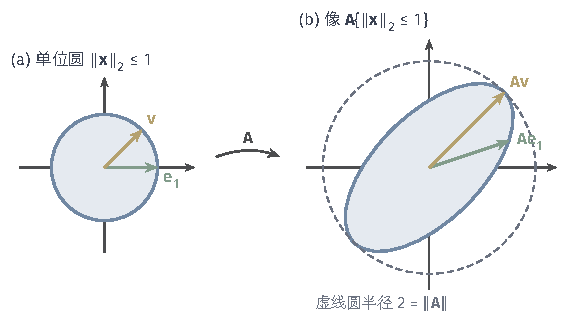
\includegraphics[width=95.1mm]{figures/02-abstract-mathematics/03-function-spaces/tikz/c2-operator-norm-stretch/figure.pdf}
  \caption{算子范数是单位球的像离原点最远的距离。(a)~平面单位圆及两个单位向量$\bm e_1$（绿）、$\bm v=(1,1)^{\top}/\sqrt2$（黄）；(b)~在$\bm A=\bigl[\begin{smallmatrix}3/2&1/2\\1/2&3/2\end{smallmatrix}\bigr]$作用下，单位圆变为旋转$45^\circ$、半轴为$2$与$1$的椭圆。$\bm A\bm e_1$的长度约为$1.58$，$\bm A\bm v$的长度为$2$，恰好触到半径为$\|\bm A\|=2$的虚线圆。}
  \label{fig:lfo-operator-norm-stretch}
\end{figure}

\paragraph{上确界未必取到}
在平面例子中，最大伸长由某个单位向量实际取到；无限维中，式~\eqref{eq:lfo-operator-norm}的上确界不一定是某个输入的输出。在$\ell^2$上令$A(x_1,x_2,x_3,\ldots)=\bigl(\tfrac12x_1,\tfrac23x_2,\tfrac34x_3,\ldots\bigr)$，即第$n$个坐标乘以$n/(n+1)$。每个坐标被乘以小于$1$的因子，故$\|Ax\|<\|x\|$对一切$x\neq0$成立；另一方面，标准单位向量满足$\|Ae_n\|=n/(n+1)\to1$，所以$\|A\|=1$，但没有任何单位向量使$\|Ax\|=1$。因此$\|A\|$应理解为“最小的统一上界”，不能无条件称为“最大输出”。

\paragraph{加权积分的范数}
回到加权积分$Wf=\int_0^1wf\,dt$，输入空间取$C([0,1])$配一致范数$\|f\|_\infty$。由$|Wf|\leq\int_0^1w|f|\,dt\leq\|f\|_\infty\int_0^1w\,dt$得$\|W\|\leq\int_0^1w\,dt$；取$f\equiv1$时等号成立，所以$\|W\|=\int_0^1w\,dt$。例如$w(t)=2t$时$\|W\|=1$。同一个读数规则若改用$L^2$范数衡量输入，算子范数会变成另一个数，第~\ref{sec:lfo-point-evaluation}节将用Hölder不等式计算。

\paragraph{求导：有界性取决于范数}
现在看求导$D$。若输入空间取$C^1([0,2\pi])$，并配上同时控制函数值与导数的范数
\[
 \|u\|_{C^1}=\|u\|_\infty+\|u'\|_\infty ,
\]
则$\|Du\|_\infty=\|u'\|_\infty\leq\|u\|_{C^1}$，$D:C^1([0,2\pi])\to C([0,2\pi])$是有界算子，$\|D\|\leq1$。取$u_n(x)=\sin(nx)/n$，有$\|Du_n\|_\infty=1$而$\|u_n\|_{C^1}=1+1/n$，比值趋于$1$，所以$\|D\|=1$；这个上确界同样不被取到，因为取到它需要$\|u\|_\infty=0$。

若在同一个函数集合$C^1([0,2\pi])$上只用一致范数$\|u\|_\infty$衡量输入，情况就完全不同。取$u_n(x)=\sin(nx)$，则
\[
 \|u_n\|_\infty=1,\qquad \|Du_n\|_\infty=\|n\cos(nx)\|_\infty=n .
\]
输出与输入的范数之比为$n$，可以任意大，所以不存在统一常数。图~\ref{fig:lfo-sine-derivative}显示了原因：振幅不变而频率升高时，函数值始终在$[-1,1]$中，斜率却按频率放大。输入上一个一致范数很小的高频扰动，可以使导数产生很大的误差。

\begin{figure}[!htb]
  \centering
  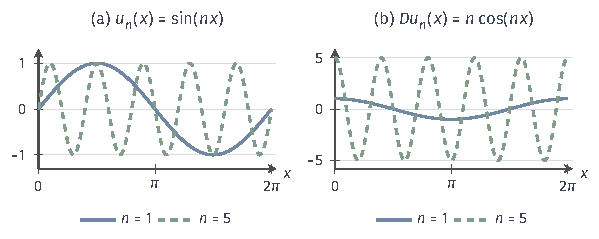
\includegraphics[width=101.5mm]{figures/02-abstract-mathematics/03-function-spaces/tikz/c2-sine-derivative/figure.pdf}
  \caption{求导对高频输入放大误差。(a)~$u_n(x)=\sin(nx)$在$n=1$（蓝实线）与$n=5$（绿虚线）时的一致范数都为$1$；(b)~导数$n\cos(nx)$的一致范数为$n$。若输入只用一致范数衡量，求导不存在统一的误差界；改用同时计入导数的$C^1$范数后，同一作用规则变为有界算子。}
  \label{fig:lfo-sine-derivative}
\end{figure}

这个例子说明，说一个算子是否有界时，必须同时交代三件事：作用规则、定义域以及定义域上的范数。把$D$看成从$C([0,2\pi])$到自身的算子时，它的定义域$D(D)=C^1([0,2\pi])$只是$C([0,2\pi])$的一个子空间，而且它在一致范数下无界，这类算子称为\term{无界算子}（unbounded operator）。对这类算子必须明确写出$D(A)$，不能把它当作已经定义在整个$X$上；第~\ref{sec:lfo-closed-graph}节还会回到求导，说明怎样选择定义域上的范数使它重新成为有界算子。

\subsection{算子的运算与算子空间}
\label{sec:lfo-operator-space}

\paragraph{加法、数乘与复合}
同一对空间之间的两个算子可以相加和数乘：对$A,B:X\to Y$及标量$\alpha$，令$(A+B)x=Ax+Bx$，$(\alpha A)x=\alpha Ax$。若$A:X\to Y$、$B:Y\to Z$，前者的输出空间正是后者的输入空间，就可以复合，$(BA)x=B(Ax)$，先作用$A$、再作用$B$，与矩阵乘积的顺序相同。这些运算都保持线性，问题是它们是否保持有界，以及范数怎样变化。

\begin{theorem}[算子运算的范数估计]
\label{thm:lfo-operator-algebra}
设$A,B:X\to Y$有界，$C:Y\to Z$有界，$\alpha\in\mathbb F$。则$A+B$、$\alpha A$与$CA$都有界，且
\[
 \|A+B\|\leq\|A\|+\|B\|,\qquad \|\alpha A\|=|\alpha|\,\|A\|,\qquad \|CA\|\leq\|C\|\,\|A\| .
\]
\end{theorem}

\begin{proof}
三个估计都先对单个输入成立，再对单位球取上确界。对$\|x\|\leq1$，由$Y$中的三角不等式，$\|(A+B)x\|\leq\|Ax\|+\|Bx\|\leq\|A\|+\|B\|$；数乘的等式直接来自范数的齐次性。复合时先用$C$的界，再用$A$的界：$\|C(Ax)\|\leq\|C\|\,\|Ax\|\leq\|C\|\,\|A\|$。
\end{proof}

复合的估计一般是严格不等式。在平面上取$\bm A=\operatorname{diag}(1,0)$、$\bm C=\operatorname{diag}(0,1)$，两者范数都是$1$，乘积却是零矩阵：$\bm A$保留的方向恰好被$\bm C$消去。每个空间都有自己的单位算子$I_X$和零算子，写复合时须分清它们属于哪个空间，例如$I_YA=A=AI_X$。

\paragraph{先投影再读数}
标量读数可以与一般变换使用同一套运算。在$H=L^2(0,1)$中，令$M$为常数函数组成的一维子空间。常数$1$是$M$中的单位向量，所以投影为$Pf=\langle1,f\rangle\cdot1=\bigl(\int_0^1f\,dt\bigr)\cdot1$。再在$M$上定义读数$\ell(c\cdot1)=c$，即读出这个常数的值。复合$\ell P:H\to\mathbb R$给出$\ell P(f)=\int_0^1f\,dt$，是一个有界线性泛函，$\|\ell P\|\leq\|\ell\|\,\|P\|=1$。

这个例子还说明了复合中定义域的作用。“读出某点的值”对一般的$L^2$等价类没有意义（第~\ref{sec:lfo-point-evaluation}节将说明原因），但$P$的输出已经落在常数函数组成的子空间中，在那里读一个值是有良定义的。复合是否合法，取决于前一个算子的输出是否落在后一个算子的定义域中，而不取决于两个规则单独看起来是否合理。

\paragraph{有界算子组成的空间}
把从$X$到$Y$的全部有界线性算子收集起来，记为$\mathcal B(X,Y)$；$X=Y$时简记$\mathcal B(X)$。由定理~\ref{thm:lfo-operator-algebra}，$\mathcal B(X,Y)$在加法和数乘下封闭，而且算子范数满足范数的三条公理（$\|A\|=0$意味着$Ax=0$对一切$x$成立，即$A=0$），所以$\mathcal B(X,Y)$本身是赋范空间。第~\ref{chap:operator-spectra-equations}章要用有限秩算子逼近一般算子、对算子级数求和，这些操作需要算子列的极限仍然留在$\mathcal B(X,Y)$中。

\begin{theorem}[算子空间的完备性]
\label{thm:lfo-operator-space-complete}
设$X$是赋范空间，$Y$是Banach空间。则$\mathcal B(X,Y)$在算子范数下是Banach空间。
\end{theorem}

证明的思路是先对每个固定输入找到输出的极限，拼成一个候选算子，再验证它线性、有界，最后把逐点收敛加强为算子范数收敛。

\begin{proof}
设$(A_n)$是$\mathcal B(X,Y)$中的Cauchy列。

\emph{第一步：逐点构造极限。}对固定的$x\in X$，$\|A_nx-A_mx\|\leq\|A_n-A_m\|\,\|x\|$，所以$(A_nx)$是$Y$中的Cauchy列。$Y$完备，于是极限存在，记为$Ax=\lim_nA_nx$。

\emph{第二步：极限映射线性且有界。}线性由极限的线性得到：$A(\alpha x+\beta z)=\lim_n(\alpha A_nx+\beta A_nz)=\alpha Ax+\beta Az$。Cauchy列有界，设$\|A_n\|\leq K$，则$\|Ax\|=\lim_n\|A_nx\|\leq K\|x\|$，故$A\in\mathcal B(X,Y)$。

\emph{第三步：算子范数收敛。}任给$\varepsilon>0$，取$N$使$n,m\geq N$时$\|A_n-A_m\|<\varepsilon$。对任意$\|x\|\leq1$及$n\geq N$，$\|A_nx-A_mx\|<\varepsilon$；固定$n$而令$m\to\infty$，得$\|A_nx-Ax\|\leq\varepsilon$。这个界对单位球上一切$x$同时成立，所以$\|A_n-A\|\leq\varepsilon$。
\end{proof}

证明只用到了输出空间$Y$的完备性，输入空间$X$不必完备。取$Y=\mathbb F$，就得到第~\ref{sec:lfo-hahn-banach}节要用的结论：任何赋范空间上的有界线性泛函全体都组成Banach空间。

\paragraph{绝对收敛的算子级数}
完备性的一个直接用途是对算子级数求和。若$A_k\in\mathcal B(X,Y)$且$\sum_k\|A_k\|<\infty$，则部分和$S_n=\sum_{k\leq n}A_k$满足$\|S_n-S_m\|\leq\sum_{k=m+1}^n\|A_k\|$（$n>m$），右端是收敛正项级数的尾部，所以$(S_n)$是Cauchy列，由定理~\ref{thm:lfo-operator-space-complete}收敛到某个$S\in\mathcal B(X,Y)$。第~\ref{sec:ose-neumann}节将用这一点对$\sum_kK^k$求和，解第二类积分方程。

\subsection{算子列的收敛}
\label{sec:lfo-operator-convergence}

上一小节在算子范数下讨论Cauchy列，这只是算子列收敛的一种方式。实际计算中更常见的情形是：用一列逐渐精细的近似算子$A_n$代替$A$，对手中的每个输入，近似输出都会越来越准。这种“对每个输入分别收敛”的要求，与“对全部单位输入同时控制误差”的要求，强弱并不相同。

\begin{definition}[强算子收敛与算子范数收敛]
\label{def:lfo-operator-convergence}
设$A_n,A\in\mathcal B(X,Y)$。若对每个$x\in X$都有$\|A_nx-Ax\|\to0$，则称$A_n$\term{强算子收敛}（strong operator convergence）到$A$；若$\|A_n-A\|\to0$，则称$A_n$\term{算子范数收敛}（convergence in operator norm）到$A$。
\end{definition}

两种收敛的量词次序不同。强算子收敛先固定输入$x$，再让$n$趋于无穷，收敛快慢可以随$x$变化；算子范数收敛要求一个只依赖$n$的误差界$\|A_n-A\|$，对单位球上的全部输入同时有效。由$\|A_nx-Ax\|\leq\|A_n-A\|\,\|x\|$，算子范数收敛蕴含强算子收敛。

强算子收敛描述的是算子列，变化的对象是算子；第~\ref{sec:lfo-weak}节的弱收敛描述的是一列空间元素，两者不能混用。下面的例子说明，强算子收敛不能反过来推出算子范数收敛。

\paragraph{截断投影$P_n\to I$}
设$H$是无限维可分Hilbert空间，$(e_k)_{k\geq1}$是第~\ref{sec:fs-orthonormal-bases}节的标准正交基，$P_n$是到$\operatorname{span}\{e_1,\ldots,e_n\}$的正交投影，$P_nx=\sum_{k\leq n}\langle e_k,x\rangle e_k$。对固定的$x$，第~\ref{sec:fs-orthogonal-expansion}节的Parseval等式给出
\[
 \|x-P_nx\|^2=\sum_{k>n}|\langle e_k,x\rangle|^2\longrightarrow0 ,
\]
因为右端是收敛级数$\sum_k|\langle e_k,x\rangle|^2=\|x\|^2$的尾部。所以$P_n$强算子收敛到单位算子$I$。

另一方面，对每个$n$，被截掉的单位向量$e_{n+1}$满足$P_ne_{n+1}=0$，于是$\|(I-P_n)e_{n+1}\|=1$。又因为$I-P_n$是到正交补的投影，$\|I-P_n\|\leq1$，所以$\|I-P_n\|=1$对一切$n$成立，$P_n$不按算子范数收敛到$I$。

图~\ref{fig:lfo-projection-strong-norm}给出了两个单位向量的截断误差。系数为$2^{-k/2}$的$x$截断误差为$2^{-n/2}$，衰减很快；系数与$1/k$成比例的$y$衰减慢得多，$n=30$时误差仍约为$0.14$。每个固定向量的误差都趋于零，但不同向量的速度可以任意慢，而被截掉的那个基向量的误差始终是$1$。这说明逐个函数可以被有限维子空间逼近，并不意味着同一个有限维子空间能以任意精度统一逼近整个单位球；第~\ref{sec:ose-finite-rank}节将看到，紧算子恰好是能被有限秩算子按算子范数逼近的那一类。

\begin{figure}[!htb]
  \centering
  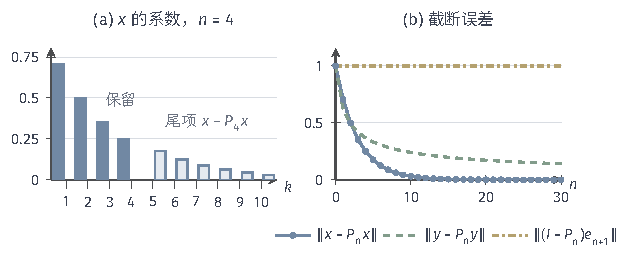
\includegraphics[width=107.2mm]{figures/02-abstract-mathematics/03-function-spaces/tikz/c2-projection-strong-norm/figure.pdf}
  \caption{截断投影的强收敛与算子范数不收敛。(a)~单位向量$x$的系数$c_k=2^{-k/2}$，$P_4$保留深色的前四项，浅色尾项构成误差$x-P_4x$；(b)~截断误差随保留项数$n$的变化：$\|x-P_nx\|=2^{-n/2}$（蓝），系数与$1/k$成比例的单位向量$y$的误差衰减较慢（绿虚线），而对被截掉的基向量$e_{n+1}$，误差始终为$1=\|I-P_n\|$（黄点划线）。}
  \label{fig:lfo-projection-strong-norm}
\end{figure}

\paragraph{有限个输入上的统一控制}
强算子收敛虽然不能控制整个单位球，对有限个输入却可以同时控制：若$x^{(1)},\ldots,x^{(m)}$是固定的输入，对每个$i$取$N_i$使误差小于$\varepsilon$，再取$N=\max_iN_i$即可。在$P_n$的例子中，失去统一控制的原因是单位球中有无穷多个相互正交的方向，每个$P_n$只能照顾其中有限个。第~\ref{sec:lfo-uniform-boundedness}节将证明，在Banach空间上，强算子收敛的算子列至少有统一的范数上界，这是算子列能被逐点控制时还剩下的统一信息。

% 第2章第2节：线性泛函的表示（积分读取与点值读取、Riesz表示、有限观测与坐标表示）。

\section{线性泛函的表示}
\label{sec:lfo-functional-representation}

本节固定标量输出，研究一个读数规则怎样写成积分权重或空间中的一个方向。顺序上先检查读数规则对空间元素是否有良定义、是否连续，再讨论表示；表示公式以这些条件为前提，不能反过来替它们作证。

\subsection{积分读取与点值读取}
\label{sec:lfo-point-evaluation}

\paragraph{加权积分读取}
最常见的读数是加权平均：给定权重$g$，读出$\int fg\,d\mu$。在测度空间$(\Omega,\mathcal F,\mu)$上取$1\leq p\leq\infty$，并设$q$是共轭指数，即$1/p+1/q=1$（$p=1$时$q=\infty$，$p=\infty$时$q=1$）。对$g\in L^q(\mu)$，令
\begin{equation}
 L_g(f)=\int_\Omega fg\,d\mu\qquad(f\in L^p(\mu)).
 \label{eq:lfo-integral-reading}
\end{equation}
第~\ref{sec:fs-holder-minkowski}节的Hölder不等式给出$|L_g(f)|\leq\int|fg|\,d\mu\leq\|f\|_p\|g\|_q$，所以积分是有限的，$L_g$是有界线性泛函，且$\|L_g\|\leq\|g\|_q$。第~\ref{sec:lfo-lp-dual}节将证明，在$\sigma$有限测度与$1\leq p<\infty$的条件下这里其实是等号。

$L_g$作用在等价类上是合理的：若$f=\tilde f$几乎处处成立，则$fg=\tilde fg$几乎处处成立，两者积分相同，所以$L_g$的值不依赖代表的选取。这一点看似平凡，却正是积分读取能够在$L^p$上使用的原因。

举一个可以复算的例子。在$L^2(0,1)$上取$g=\mathbf 1_{[0,1/2]}$，$L_g(f)=\int_0^{1/2}f\,dt$读出前半段的累计。Hölder不等式给出$\|L_g\|\leq\|g\|_2=1/\sqrt2$；取$f=g$，则$L_g(g)=1/2$而$\|g\|_2=1/\sqrt2$，比值正好是$1/\sqrt2$，所以$\|L_g\|=1/\sqrt2$。同一规则在$C([0,1])$的一致范数下的范数是$1/2$（取$f\equiv1$），两个数不同，因为输入误差的衡量方式不同。

\paragraph{连续函数的点值读取}
另一类读数是读出某一点的值。设$K$是紧致度量空间，$x\in K$固定。在$C(K)$上配一致范数，令$\delta_x(f)=f(x)$，称为在$x$处的\term{点值泛函}（point evaluation functional）。由$|f(x)|\leq\sup_K|f|=\|f\|_\infty$，$\delta_x$是有界线性泛函，$\|\delta_x\|\leq1$；取$f\equiv1$得$\|\delta_x\|=1$。

两种读数都输出一个标量，但依靠的空间结构不同：积分读取依靠积分对零测集不敏感，点值读取依靠一致范数对每一点都有控制。把点值读取搬到积分空间中，这两种结构就发生冲突。

\paragraph{等价类上没有点值}
在Lebesgue测度下的$L^p(0,1)$中，单点$\{x_0\}$的测度为零。改变一个函数在$x_0$处的值，得到的函数与原函数几乎处处相等，属于同一个等价类，例如$f$与$f+\mathbf 1_{\{x_0\}}$。同一个等价类在$x_0$处可以有任何值，所以“读出$x_0$处的值”在$L^p$上根本没有良定义，谈不上是否有界。

\paragraph{窄尖峰：连续代表也不够}
或许可以只考虑连续函数，因为连续代表若存在则唯一。但即使把对象限制在$C([0,1])$中、用$L^2$范数衡量误差，点值仍然不受控制。取贴着左端点、宽为$1/n$、高为$1$的尖峰
\[
 \tau_n(t)=\max(1-nt,\,0)\qquad(t\in[0,1]).
\]
它连续，$\delta_0(\tau_n)=\tau_n(0)=1$，而直接积分得
\[
 \|\tau_n\|_2^2=\int_0^{1/n}(1-nt)^2\,dt=\frac{1}{3n}\longrightarrow0 .
\]
图~\ref{fig:lfo-point-spike}画出了$n=4,10,25$三个尖峰：$L^2$范数从约$0.289$降到约$0.115$，左端点的值始终是$1$。所以不存在常数$C$使$|f(0)|\leq C\|f\|_2$对一切连续$f$成立，点值泛函在$(C([0,1]),\|\cdot\|_2)$上无界。

\begin{figure}[!htb]
  \centering
  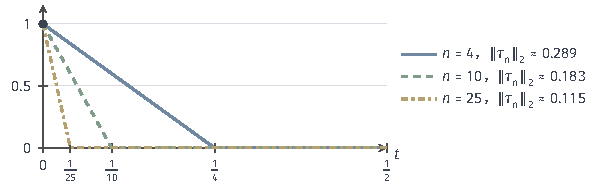
\includegraphics[width=101.7mm]{figures/02-abstract-mathematics/03-function-spaces/tikz/c2-point-spike/figure.pdf}
  \caption{窄尖峰使点值不受$L^2$范数控制。尖峰$\tau_n(t)=\max(1-nt,0)$在$n=4,10,25$时的图像（蓝实线、绿虚线、黄点划线）。左端点的值恒为$1$（黑点），而$\|\tau_n\|_{L^2(0,1)}=1/\sqrt{3n}$随$n$增大趋于零。}
  \label{fig:lfo-point-spike}
\end{figure}

\paragraph{原子测度改变结论}
上面的困难来自单点的测度为零。若测度在$x_0$处有正的质量，结论就会改变。在$[0,1]$上取$\mu=\lambda+\delta_{x_0}$，其中$\lambda$是Lebesgue测度，$\delta_{x_0}$是集中在$x_0$的单位质量。此时$\mu(\{x_0\})=1$，改变$x_0$处的值会改变等价类，于是$f(x_0)$对$L^2(\mu)$的元素有良定义，并且
\[
 |f(x_0)|^2=\int_{\{x_0\}}|f|^2\,d\mu\leq\int|f|^2\,d\mu=\|f\|_{L^2(\mu)}^2 .
\]
正测度的单点原子与零测单点必须区分。一般的积分空间不支持点值读取；第~\ref{chap:rkhs}章将专门研究点值读取连续的Hilbert函数空间，第~\ref{sec:sob-embedding}节则说明控制导数能在什么条件下恢复点值的连续性。

\subsection{Hilbert空间中的Riesz表示}
\label{sec:lfo-riesz}

\paragraph{每个方向给出一个读数}
在Hilbert空间$H$中，任取$h\in H$，令$L_h(f)=\langle h,f\rangle$。按全书的约定，内积对第二个变量线性，所以$L_h$是线性泛函。Cauchy--Schwarz不等式给出$|L_h(f)|\leq\|h\|\,\|f\|$，即$\|L_h\|\leq\|h\|$；$h\neq0$时取$f=h/\|h\|$，得$L_h(f)=\|h\|$，于是$\|L_h\|=\|h\|$。每个方向都是一个读数规则，读数的范数等于方向的长度。

反过来的问题更有用：给定一个有界线性读数$L$，是否一定存在方向$h$，使读数就是与$h$做内积？若是，就可以用空间中的几何（正交、投影、长度）来研究读数。

\paragraph{核与正交方向}
先观察一个非零有界线性泛函$L$的核$N=\ker L=\{f:L(f)=0\}$。它是线性子空间；又因为$L$连续，若$f_n\in N$且$f_n\to f$，则$L(f)=\lim L(f_n)=0$，所以$N$是闭子空间。$N$还“只差一维”：任取$w\notin N$，每个$f$都可以写成
\[
 f=\Bigl(f-\frac{L(f)}{L(w)}w\Bigr)+\frac{L(f)}{L(w)}w ,
\]
括号中的元素在$L$下的值为零，属于$N$。所以$H=N+\operatorname{span}\{w\}$。若进一步把$w$取在$N$的正交补中，读数$L(f)$就只取决于$f$沿$w$方向的分量，这正是表示向量的来源。由此得到的结论称为\term{Riesz表示定理}（Riesz representation theorem）。

\begin{theorem}[Riesz表示定理]
\label{thm:lfo-riesz}
设$H$是Hilbert空间，$L:H\to\mathbb F$是有界线性泛函。则存在唯一的$h_L\in H$，使
\begin{equation}
 L(f)=\langle h_L,f\rangle\qquad(f\in H),
 \label{eq:lfo-riesz}
\end{equation}
并且$\|L\|=\|h_L\|$。
\end{theorem}

证明分三步：用投影找出与核正交的方向，用这个方向写出表示，再验证唯一性与范数等式。

\begin{proof}
$L=0$时取$h_L=0$。下设$L\neq0$，于是闭子空间$N=\ker L$不是全空间。

\emph{第一步：找与核正交的方向。}取$v$使$L(v)\neq0$。由第~\ref{sec:fs-projection}节的正交投影定理，$v=P_Nv+w$，其中$P_Nv\in N$，$w=v-P_Nv\perp N$。由$L(w)=L(v)-L(P_Nv)=L(v)\neq0$知$w\neq0$。

\emph{第二步：写出表示。}对任意$f\in H$，前面已说明$f-\frac{L(f)}{L(w)}w\in N$，它与$w$正交：
\[
 0=\Bigl\langle w,\ f-\frac{L(f)}{L(w)}w\Bigr\rangle=\langle w,f\rangle-\frac{L(f)}{L(w)}\|w\|^2 .
\]
这里用到内积对第二个变量线性。解出$L(f)=\frac{L(w)}{\|w\|^2}\langle w,f\rangle$。令
\begin{equation}
 h_L=\frac{\overline{L(w)}}{\|w\|^2}\,w ,
 \label{eq:lfo-riesz-direction}
\end{equation}
由于内积对第一个变量共轭线性，$\langle h_L,f\rangle=\frac{L(w)}{\|w\|^2}\langle w,f\rangle=L(f)$。

\emph{第三步：唯一性与范数。}若$h,h'$都满足式~\eqref{eq:lfo-riesz}，则$\langle h-h',f\rangle=0$对一切$f$成立，取$f=h-h'$得$h=h'$。范数等式正是本小节开头对$L_h$的计算。
\end{proof}

式~\eqref{eq:lfo-riesz-direction}中的共轭在实空间中消失；在复空间中，它使对应$L\mapsto h_L$是共轭线性的：$h_{\alpha L}=\bar\alpha h_L$。这是内积对第一个变量共轭线性这一约定的直接后果。

\paragraph{读数的几何}
图~\ref{fig:lfo-riesz-kernel}在实平面的二维截面上画出了这个构造。核$N$是一条过原点的直线，表示向量$h_L$与它垂直；读数相等的点组成平行于$N$的直线，读数每增加$\|h_L\|^2$，水平线沿$h_L$方向平移一个$\|h_L\|$的距离。任何$f$都分解为$N$中的分量与沿$h_L$的分量，前者对读数没有贡献，后者的长度决定读数。读数大的方向就是$h_L$本身，这也解释了$\|L\|=\|h_L\|$：在单位球上，沿$h_L$方向的单位向量读到的值最大。

\begin{figure}[!htb]
  \centering
  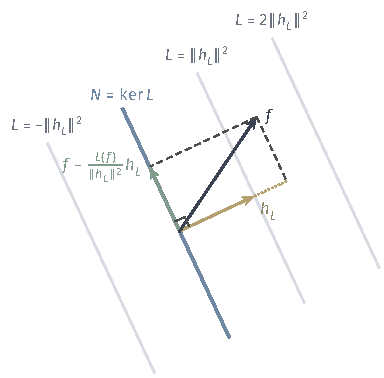
\includegraphics[width=65.1mm]{figures/02-abstract-mathematics/03-function-spaces/tikz/c2-riesz-kernel/figure.pdf}
  \caption{Riesz表示的几何示意（实空间中的二维截面）。核$N=\ker L$（蓝线）是闭子空间，表示向量$h_L$（黄）与之正交；灰线是读数$L=c$的水平集，平行于$N$。元素$f$减去沿$h_L$的分量$\frac{L(f)}{\|h_L\|^2}h_L$后落入$N$（绿），因此读数只由$f$沿$h_L$方向的分量决定。}
  \label{fig:lfo-riesz-kernel}
\end{figure}

\paragraph{$L^2$中的读数与方向}
在$L^2(0,1)$中，几个熟悉的读数对应的方向都可以直接写出。整体平均$L(f)=\int_0^1f\,dt=\langle1,f\rangle$对应常数$h_L=1$，$\|L\|=1$。前半段平均$L(f)=2\int_0^{1/2}f\,dt$对应$h_L=2\cdot\mathbf 1_{[0,1/2]}$，$\|L\|=\|h_L\|_2=2\cdot(1/2)^{1/2}=\sqrt2$。加权读数$L(f)=\int_0^1tf(t)\,dt$对应$h_L(t)=t$，$\|L\|=(\int_0^1t^2\,dt)^{1/2}=1/\sqrt3$。正交展开中的第$k$个系数$f\mapsto\langle e_k,f\rangle$对应$h_L=e_k$。抽象的读数规则由此变成了与一个固定函数的比较，读数的大小就是$f$与这个函数的相关程度。

\paragraph{表示以有界为前提}
Riesz表示定理需要两个前提，缺一不可。第一，$L$必须已经有界。在$C([0,1])$上配$L^2$内积，点值$\delta_0$无界；它也确实没有表示函数：若有连续$h$使$f(0)=\int_0^1hf\,dt$对一切连续$f$成立，代入尖峰$\tau_n$，左端恒为$1$，右端的绝对值不超过$\|h\|_2\|\tau_n\|_2\to0$，矛盾。定理不能替点值读取证明连续性，连续性必须事先单独检验。

第二，空间必须完备。仍在$C([0,1])$上配$L^2$内积，读数$L(f)=\int_0^{1/2}f\,dt$满足$|L(f)|\leq\|f\|_2/\sqrt2$，是有界的。在完备的$L^2(0,1)$中它的表示方向是$\mathbf 1_{[0,1/2]}$，但这个函数没有连续代表，不在$C([0,1])$中。所以在不完备的内积空间里，有界读数可以没有表示向量；证明中用到的正交投影定理依赖完备性，此处失效。

最后，Riesz表示只处理标量输出。输出为向量的观测，例如同时读出两个端点值$(f(0),f(1))$，要逐个分量作为标量泛函处理，各分量分别有自己的表示方向（若它们有界），不能未经说明就当作一个泛函。

\subsection{有限观测与坐标表示}
\label{sec:lfo-finite-observations}

实际中我们只能对函数做有限次读数，并且常把候选函数限制在一个有限维空间里。本小节说明在这种设定下，读数、坐标和函数之间怎样用矩阵联系，以及有限条读数能否唯一确定一个函数。

\paragraph{观测矩阵}
设候选函数属于有限维子空间$V=\operatorname{span}\{\varphi_1,\ldots,\varphi_m\}$，其中$\varphi_1,\ldots,\varphi_m$线性无关，每个$f\in V$唯一地写成$f=\sum_{j=1}^mc_j\varphi_j$，系数向量记为$\bm c=(c_1,\ldots,c_m)^{\top}$。再设$L_1,\ldots,L_n$是$V$上的线性读数。由线性，
\[
 L_i(f)=\sum_{j=1}^mc_jL_i(\varphi_j)\qquad(i=1,\ldots,n).
\]
令$\bm A\in\mathbb F^{n\times m}$，$\bm A_{i,j}=L_i(\varphi_j)$，称为\term{观测矩阵}（observation matrix），则读数向量$\bm r=(L_1(f),\ldots,L_n(f))^{\top}$满足
\begin{equation}
 \bm r=\bm A\bm c .
 \label{eq:lfo-observation-matrix}
\end{equation}
矩阵的第$i$行是第$i$条读数规则在各个基函数上的取值，第$j$列是第$j$个基函数在全部读数下留下的记录。点值读数给出$\bm A_{i,j}=\varphi_j(x_i)$，积分读数给出$\bm A_{i,j}=\int\varphi_jg_i\,d\mu$；代入之前仍须核对每条读数在$V$上有良定义。

\paragraph{仿射函数的两次读数}
取$V$为$[0,1]$上的仿射函数，基为$\varphi_1=1$、$\varphi_2=t$，$f=c_1+c_2t$。读$f(0)$与$f(1)$时，
\[
 \bm A=\begin{bmatrix}1&0\\1&1\end{bmatrix},\qquad
 \begin{bmatrix}f(0)\\f(1)\end{bmatrix}=\bm A\begin{bmatrix}c_1\\c_2\end{bmatrix}.
\]
$\bm A$可逆，由$c_1=f(0)$、$c_2=f(1)-f(0)$恢复系数。若只读$f(0)$，$\bm A=[1\ \ 0]$，第二列为零：斜率方向在记录中完全看不见。若改读$f(0)$与整体平均$\int_0^1f\,dt$，第二行变为$(1,1/2)$，矩阵仍可逆。图~\ref{fig:lfo-observation-matrix}(a)(b)对比了一次与两次点值读数的情形。

\paragraph{非标准正交基下的Gram矩阵}
坐标向量$\bm c$与函数$f$一一对应，但坐标的欧氏长度一般不是函数的范数。在内积空间中，记\term{Gram矩阵}（Gram matrix）$\bm G_{j,k}=\langle\varphi_j,\varphi_k\rangle$，则对$f=\sum_jc_j\varphi_j$、$u=\sum_kd_k\varphi_k$有
\[
 \langle f,u\rangle=\sum_{j,k}\bar c_jd_k\langle\varphi_j,\varphi_k\rangle=\bm c^{\mathsf H}\bm G\bm d ,
\]
其中$\bm c^{\mathsf H}$是共轭转置，实情形即$\bm c^{\top}$。只有基标准正交时$\bm G=\bm I$，函数内积才等于系数内积。

仍以$L^2(0,1)$中的基$1,t$为例，$\bm G=\bigl[\begin{smallmatrix}1&1/2\\1/2&1/3\end{smallmatrix}\bigr]$。函数$f=t-1/2$的系数为$\bm c=(-1/2,1)^{\top}$，于是$\|f\|_2^2=\bm c^{\top}\bm G\bm c=\tfrac14-\tfrac12+\tfrac13=\tfrac1{12}$，与直接积分$\int_0^1(t-1/2)^2\,dt=1/12$一致；而系数的欧氏长度平方是$5/4$，差了十五倍。在坐标中计算误差或正交性时，必须带上$\bm G$。

\paragraph{唯一恢复的条件}
读数能否唯一确定候选空间中的函数，归结为观测矩阵的列是否线性无关。

\begin{theorem}[有限维候选的唯一恢复]
\label{thm:lfo-finite-recovery}
设$V$与$L_1,\ldots,L_n$如上，$\bm A$为观测矩阵。则读数向量唯一确定$V$中的函数，当且仅当$\bm A$满列秩，即$\operatorname{rank}\bm A=m$。特别地，这要求$n\geq m$。
\end{theorem}

\begin{proof}
两个候选$f=\sum c_j\varphi_j$与$u=\sum d_j\varphi_j$给出相同读数，当且仅当$\bm A(\bm c-\bm d)=\bm 0$。所以读数唯一确定函数，当且仅当$\bm A\bm z=\bm 0$只有零解，即$\bm A$的$m$列线性无关；这又等价于秩为$m$，而秩不超过行数$n$。
\end{proof}

结论严格限定在给定的候选空间$V$上。图~\ref{fig:lfo-observation-matrix}(c)把候选扩大到二次多项式：基$1,t,t(t-1)$下，两次点值读数的观测矩阵为$\bigl[\begin{smallmatrix}1&0&0\\1&1&0\end{smallmatrix}\bigr]$，第三列为零，函数$t(t-1)$在$t=0,1$处都等于零，在两次读数中看不见。于是$1+t+s\,t(t-1)$对一切$s$给出相同的记录。

\begin{figure}[!htb]
  \centering
  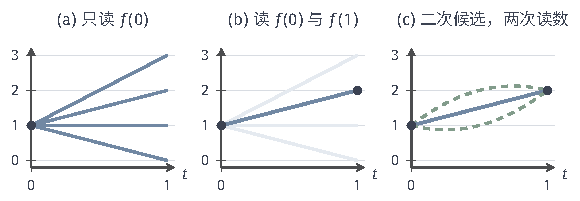
\includegraphics[width=98.2mm]{figures/02-abstract-mathematics/03-function-spaces/tikz/c2-observation-matrix/figure.pdf}
  \caption{有限读数能否确定候选函数。(a)~仿射候选$f=1+bt$（$b=-1,0,1,2$）都满足$f(0)=1$，一次读数无法区分；(b)~再读$f(1)=2$，只剩$b=1$（深蓝线），观测矩阵满列秩；(c)~候选扩大为二次多项式后，$1+t+s\,t(t-1)$（$s=-2,0,2$）在$t=0,1$处的读数完全相同，方向$t(t-1)$不可见。}
  \label{fig:lfo-observation-matrix}
\end{figure}

\paragraph{无限维中有限读数不够}
若候选空间是无限维的，有限条读数永远不能唯一确定函数。线性映射$f\mapsto(L_1(f),\ldots,L_n(f))$从候选空间映到$\mathbb F^n$；它的核若只含零，就会把一个无限维空间单射地放进$n$维空间，这不可能。所以总有非零的$f$使全部读数为零，加到任何候选上都不改变记录。上面的$t(t-1)$只是这种不可见方向在二次多项式中的具体样子。

本小节只建立空间元素、坐标与读数之间的对应。读数带有噪声或彼此不相容时，$\bm r=\bm A\bm c$可能无解，需要另选拟合准则与误差度量；这属于优化问题，可参考\BookChapterRef{chap:optimization}{卷三“优化问题的定义与基本性质”章}。第~\ref{sec:rkhs-finite-observations}节将在点值连续的核空间中，用Riesz表示方向重新组织有限观测。

% 第2章第3节：对偶空间（对偶空间与Hahn--Banach延拓、积分空间的对偶、连续函数空间与测度表示）。

\section{对偶空间}
\label{sec:lfo-dual}

上一节逐个研究读数规则，本节把同一空间上的全部有界线性读数收集成一个空间。我们关心两个问题：这些读数是否多到足以区分任意两个不同的元素，以及在具体的函数空间中，它们究竟长什么样。前一个问题由延拓定理回答，适用于一切赋范空间；后一个问题要按原空间的类型分别回答。

\subsection{对偶空间与泛函延拓}
\label{sec:lfo-hahn-banach}

\begin{definition}[对偶空间]
\label{def:lfo-dual-space}
赋范空间$X$上全部有界线性泛函组成的空间$X^*=\mathcal B(X,\mathbb F)$称为$X$的\term{对偶空间}（dual space），配以泛函范数$\|L\|=\sup_{\|x\|\leq1}|L(x)|$。
\end{definition}

标量域$\mathbb F$是完备的，所以由定理~\ref{thm:lfo-operator-space-complete}，无论$X$本身是否完备，$X^*$总是Banach空间。例如在不完备的多项式空间上配一致范数，它的对偶空间仍然完备。

\paragraph{读数规则与向量表示不是一回事}
对偶空间的元素是读数规则，不是原空间的元素。即使在有限维中，两者的范数也可能不同。在$\mathbb R^2$上配$\ell^1$范数$\|\bm x\|_1=|x_1|+|x_2|$，每个线性泛函都写成$L(\bm x)=a_1x_1+a_2x_2$。由$|L(\bm x)|\leq\max(|a_1|,|a_2|)\,\|\bm x\|_1$，且在$\bm x=\bm e_1$或$\bm e_2$处等号可以成立，得$\|L\|=\max(|a_1|,|a_2|)$。系数向量$\bm a$属于$\mathbb R^2$，但它作为读数的长度要用$\ell^\infty$范数计算，这是\term{对偶范数}（dual norm）的一个例子。

Hilbert空间是特殊情形：Riesz表示定理把每个读数对应到唯一的向量$h_L$，并且$\|L\|=\|h_L\|$，所以$H^*$与$H$可以通过保范数的（复情形下共轭线性的）双射视为同一个空间。对一般空间不能直接写$X^*=X$；第~\ref{sec:lfo-lp-dual}节会看到，$L^p$的对偶在$p\neq2$时由另一个空间$L^q$表示。

\paragraph{读数够不够区分元素}
在Hilbert空间中，若$x\neq0$，读数$\langle x,\cdot\rangle$在$x$处给出$\|x\|^2\neq0$，所以总有连续读数能把$x$与$0$区分开。一般的Banach空间没有内积，无法直接写出这样的读数。我们能做的是先在包含$x$的一维子空间上定义一个读数，再设法把它延拓到全空间，并且不增大它的范数。保证这种延拓存在的是\term{Hahn--Banach定理}（Hahn--Banach theorem）。

\begin{theorem}[Hahn--Banach定理（保范数延拓）]
\label{thm:lfo-hahn-banach}
设$X$是赋范空间，$M\subset X$是线性子空间，$\ell:M\to\mathbb F$是有界线性泛函。则存在$L\in X^*$，使$L|_M=\ell$且$\|L\|=\|\ell\|$。
\end{theorem}

\paragraph{延拓一维：可选范围非空}
以实空间为例看延拓的核心一步。不妨设$\|\ell\|=1$，任取$z\notin M$，要把$\ell$延拓到$M\oplus\operatorname{span}\{z\}$上。线性延拓完全由一个数$t=L(z)$决定：$L(m+sz)=\ell(m)+st$。要求$\|L\|\leq1$，即$|\ell(m)+st|\leq\|m+sz\|$对一切$m\in M$、$s\in\mathbb R$成立。$s=0$时这就是$\|\ell\|\leq1$；$s\neq0$时两边除以$|s|$并把$m/s$重新记为$m$，条件化为
\[
 -\|m+z\|-\ell(m)\leq t\leq\|m+z\|-\ell(m)\qquad(m\in M).
\]
这样的$t$存在，当且仅当左端对$m$的上确界不超过右端对$m'$的下确界，即对一切$m,m'\in M$，
\[
 -\|m+z\|-\ell(m)\leq\|m'+z\|-\ell(m') .
\]
这确实成立，因为$\ell(m')-\ell(m)=\ell(m'-m)\leq\|m'-m\|\leq\|m'+z\|+\|m+z\|$，移项即得。所以可选的$t$组成一个非空区间，任取其中一个就把$\ell$保范数地延拓了一维。

\paragraph{从一维到全空间（补充）}
若$X$可分，取可数稠密集$\{z_1,z_2,\ldots\}$，逐个把$z_k$添进定义域并重复上面的一步，就把$\ell$保范数地延拓到$\operatorname{span}(M\cup\{z_k\})$上；这个子空间稠密，延拓后的泛函一致连续，可以唯一地连续延拓到整个$X$，范数不变。不可分时，“逐个添加”需要用Zorn引理代替归纳法，思路相同。复空间的情形可以先延拓实部$\operatorname{Re}\ell$，再由$L(x)=\operatorname{Re}L(x)-i\operatorname{Re}L(ix)$恢复复线性泛函。这些细节属于补充，主线只需记住条件（$\ell$在子空间上有界）和结论（全空间上存在范数相同的延拓）。

\paragraph{延拓可以不唯一}
图~\ref{fig:lfo-hahn-banach}展示了一维延拓中的那个“非空区间”。在$(\mathbb R^2,\|\cdot\|_1)$中取$M$为横轴，$\ell(s,0)=s$，$\|\ell\|=1$。延拓为$L_t(\bm x)=x_1+tx_2$，由前面对偶范数的计算，$\|L_t\|=\max(1,|t|)$，所以$|t|\leq1$的每个$t$都给出保范数延拓。几何上，水平线$\{L_t=1\}$都经过点$(1,0)$并支撑菱形单位球；菱形在这个顶点处有许多支撑线，延拓因而不唯一。在欧氏范数下，单位圆在$(1,0)$只有一条切线$x_1=1$，延拓唯一。一般地，Hilbert空间中的保范数延拓是唯一的，就是$L=\ell\circ P_{\overline M}$（$\ell$先连续延拓到闭包$\overline M$上）。

\begin{figure}[!htb]
  \centering
  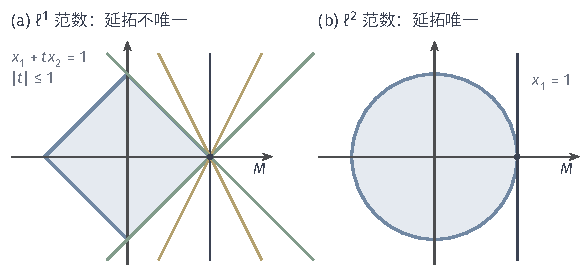
\includegraphics[width=98.9mm]{figures/02-abstract-mathematics/03-function-spaces/tikz/c2-hahn-banach/figure.pdf}
  \caption{保范数延拓与单位球的支撑线。(a)~$(\mathbb R^2,\|\cdot\|_1)$的单位球是菱形，子空间$M$为横轴，$\ell(s,0)=s$。延拓$L_t(\bm x)=x_1+tx_2$在$|t|\leq1$时范数都为$1$，对应的水平线$x_1+tx_2=1$（图中$t=0,\pm\frac12,\pm1$）都过$(1,0)$并支撑菱形；(b)~欧氏单位圆在$(1,0)$只有一条支撑线$x_1=1$，保范数延拓唯一。}
  \label{fig:lfo-hahn-banach}
\end{figure}

\paragraph{读数足以区分元素}
把定理用于一维子空间，就得到本小节开头的问题的答案。

\begin{theorem}[范数的对偶刻画]
\label{thm:lfo-norming-functional}
设$X$是赋范空间，$x\in X$且$x\neq0$。则存在$L\in X^*$，使$\|L\|=1$且$L(x)=\|x\|$。因此对一切$x\in X$，
\begin{equation}
 \|x\|=\sup_{\|L\|\leq1}|L(x)|=\max_{\|L\|\leq1}|L(x)| ,
 \label{eq:lfo-norm-dual}
\end{equation}
并且若$L(x)=L(z)$对一切$L\in X^*$成立，则$x=z$。
\end{theorem}

\begin{proof}
在$M=\operatorname{span}\{x\}$上令$\ell(\alpha x)=\alpha\|x\|$，则$|\ell(\alpha x)|=\|\alpha x\|$，$\|\ell\|=1$。由定理~\ref{thm:lfo-hahn-banach}延拓得到所需的$L$。对一切$\|L'\|\leq1$有$|L'(x)|\leq\|x\|$，而上面的$L$取到等号，故式~\eqref{eq:lfo-norm-dual}成立（$x=0$时两边为零）。最后，若$x\neq z$，对$x-z$取这样的$L$，得$L(x)-L(z)=\|x-z\|\neq0$。
\end{proof}

式~\eqref{eq:lfo-norm-dual}说，一个元素的长度可以由单位读数的最大读值完全恢复。在具体空间中，取到最大值的读数常常可以直接写出。例如在$C([0,1])$中，设$|f|$在$t_0$处取到最大值，则$L=\operatorname{sgn}(f(t_0))\,\delta_{t_0}$就满足$\|L\|=1$、$L(f)=\|f\|_\infty$。定理的价值在于，即使写不出这样的读数，它也保证存在。

凸集的分离、优化问题的对偶以及最优性条件，都是同一延拓思想的几何形式，属于优化问题，可参考\BookChapterRef{chap:constrained-optimization}{卷三“有约束优化的求解”章}。

\subsection{积分空间的对偶}
\label{sec:lfo-lp-dual}

第~\ref{sec:lfo-point-evaluation}节用Hölder不等式说明，每个$g\in L^q$都给出$L^p$上的有界读数$L_g$。本小节回答反方向的问题：$L^p$上的每个有界读数是否都来自某个权重$g$，权重的范数又是否等于读数的范数。为避免共轭记号，先在实值函数上讨论，复情形在小节末交代。

\begin{theorem}[$L^p$的对偶]
\label{thm:lfo-lp-dual}
设$(\Omega,\mathcal F,\mu)$是$\sigma$有限测度空间，$1\leq p<\infty$，$q$为共轭指数。则映射$g\mapsto L_g$，$L_g(f)=\int_\Omega fg\,d\mu$，是从$L^q(\mu)$到$(L^p(\mu))^*$的保范数线性双射，即每个$L\in(L^p)^*$都唯一地写成$L=L_g$，且$\|L\|=\|g\|_q$。
\end{theorem}

证明分两部分：正向说明$\|L_g\|$恰好等于$\|g\|_q$，反向说明每个读数都有这样的权重。

\paragraph{正向：等号由哪个输入取到}
Hölder不等式已给出$\|L_g\|\leq\|g\|_q$，只需找输入取到或逼近等号。设$1<p<\infty$，$g\neq0$。令$f=|g|^{q-1}\operatorname{sgn}(g)$，则$fg=|g|^q$，并且$|f|^p=|g|^{(q-1)p}=|g|^q$（因为$(q-1)p=q$）。于是
\[
 \begin{aligned}
 &L_g(f)=\int|g|^q\,d\mu=\|g\|_q^q,\qquad \|f\|_p=\|g\|_q^{q/p},\\
 &\frac{L_g(f)}{\|f\|_p}=\|g\|_q^{\,q-q/p}=\|g\|_q .
 \end{aligned}
\]
$p=1$、$q=\infty$时等号未必取到，改用逼近：对$\varepsilon>0$，集合$E=\{|g|>\|g\|_\infty-\varepsilon\}$测度为正；由$\sigma$有限，可取$E$中测度有限且为正的部分$E'$，令$f=\operatorname{sgn}(g)\mathbf 1_{E'}/\mu(E')$，则$\|f\|_1=1$而$L_g(f)\geq\|g\|_\infty-\varepsilon$。正向保范数说明映射$g\mapsto L_g$单射。

\paragraph{反向：由读数生成测度}
先设$\mu$有限。给定$L\in(L^p)^*$，对可测集$E$令$\nu(E)=L(\mathbf 1_E)$。证明$\nu$是有限符号测度并对$\mu$绝对连续，就可以调用Radon--Nikodym定理。

有限可加性来自$L$的线性：不交时$\mathbf 1_{E\cup F}=\mathbf 1_E+\mathbf 1_F$。可数可加性来自$L$的连续性，这里用到$p<\infty$：若$E=\bigcup_kE_k$为不交并，则
\[
 \Bigl\|\mathbf 1_E-\sum_{k\leq n}\mathbf 1_{E_k}\Bigr\|_p=\mu\Bigl(\bigcup_{k>n}E_k\Bigr)^{1/p}\longrightarrow0 ,
\]
所以$\sum_{k\leq n}\nu(E_k)\to\nu(E)$。绝对连续性同样直接：$\mu(E)=0$时$\mathbf 1_E$是$L^p$中的零元，$\nu(E)=L(0)=0$。由第~\ref{sec:measure-signed-total-variation}节的Jordan分解（定理~\ref{thm:measure-hahn-jordan}），$\nu$是两个有限测度之差，二者都对$\mu$绝对连续；分别应用Radon--Nikodym定理（定理~\ref{thm:measure-radon-nikodym}），得到可积函数$g$使
\[
 L(\mathbf 1_E)=\int_Eg\,d\mu\qquad(E\in\mathcal F).
\]

\paragraph{反向：从示性函数推广到全空间}
由线性，$L(f)=\int fg\,d\mu$对简单函数$f$成立。接下来说明$g\in L^q$，并把等式推广到全部$L^p$。对$1<p<\infty$，令$E_n=\{|g|\leq n\}$，$f_n=|g|^{q-1}\operatorname{sgn}(g)\mathbf 1_{E_n}$。$f_n$是有界可测函数，可由简单函数一致逼近；在有限测度下一致收敛蕴含$L^p$收敛，两端都随之收敛，所以等式对$f_n$也成立。于是
\[
 \int_{E_n}|g|^q\,d\mu=L(f_n)\leq\|L\|\,\|f_n\|_p=\|L\|\Bigl(\int_{E_n}|g|^q\,d\mu\Bigr)^{1/p},
\]
整理得$(\int_{E_n}|g|^q)^{1/q}\leq\|L\|$。令$n\to\infty$，由单调收敛定理，$\|g\|_q\leq\|L\|$。$p=1$时可类似地在$\{|g|>\|L\|\}$上取示性函数说明该集合零测。既然$g\in L^q$，$L$与$L_g$都是$L^p$上的连续泛函，又在简单函数上相等；第~\ref{sec:fs-density-separability}节说明简单函数在$L^p$中稠密，所以$L=L_g$。

\paragraph{$\sigma$有限情形（补充）}
一般的$\sigma$有限测度把$\Omega$分成可数个测度有限的不交片$\Omega_k$。在每一片上得到$g_k$，由唯一性它们彼此相容，拼成$g=\sum_kg_k\mathbf 1_{\Omega_k}$；对每个有限并的范数估计都不超过$\|L\|$，再用单调收敛得$\|g\|_q\leq\|L\|$。$p=1$时$\sigma$有限不能去掉，$1<p<\infty$时则可以用更细的论证去掉这一假设，这里不展开。

\paragraph{复值函数的配对}
复值情形下，为与内积约定一致，把配对写成$L_g(f)=\int\bar gf\,d\mu$，即对权重取共轭、对输入线性。$p=2$时它正是$\langle g,f\rangle$，定理~\ref{thm:lfo-lp-dual}回到Riesz表示定理。正向构造中的$\operatorname{sgn}(g)$相应换为$g/|g|$（$g=0$处取零）。

\paragraph{一个可复算的范数}
在$L^3(0,1)$上取读数$L(f)=\int_0^1tf(t)\,dt$。共轭指数$q=3/2$，由定理~\ref{thm:lfo-lp-dual}，
\[
 \|L\|=\|t\|_{3/2}=\Bigl(\int_0^1t^{3/2}\,dt\Bigr)^{2/3}=\Bigl(\frac25\Bigr)^{2/3}\approx0.543 ,
\]
取到范数的输入是$f(t)=t^{q-1}=t^{1/2}$。同一个权重在$L^2$中的读数范数是$\|t\|_2=1/\sqrt3\approx0.577$，在$L^1$中是$\|t\|_\infty=1$：指数$p$越小，$L^p$范数对集中在小区域上的输入越宽容，读数相对于它的放大就可能越大。

\paragraph{端点：$L^\infty$的对偶更大}
定理排除了$p=\infty$，这不是技术上的疏漏。$L^1$的对偶是$L^\infty$，但$L^\infty$的对偶一般不能全部由$L^1$表示。以计数测度下的$\ell^\infty$为例。在收敛数列组成的子空间$c$上定义$\ell(x)=\lim_nx_n$，它的范数为$1$。由Hahn--Banach定理，它延拓为某个$L\in(\ell^\infty)^*$。若$L$由某个$g\in\ell^1$表示，即$L(x)=\sum_kg_kx_k$，则由标准单位向量满足$L(e_k)=\lim_n(e_k)_n=0$得每个$g_k=0$，于是$L=0$；可是$L$在常数列$(1,1,\ldots)$上的值为$1$，矛盾。所以$(\ell^\infty)^*$严格大于$\ell^1$；对Lebesgue测度下的$L^\infty(0,1)$也有类似的构造。

这一端点限制为第~\ref{sec:lfo-reflexive}节的反射性和第~\ref{sec:lfo-weak-star}节的弱星收敛保留了准确的入口。有限维和$L^2$中“对偶就是自身”的直觉，不能直接推广到所有积分空间。

\subsection{连续函数空间与测度表示（补充）}
\label{sec:lfo-ck-dual}

本小节转到另一类空间$C(K)$，其中$K$是紧致度量空间，配一致范数，只考虑实值函数。它的读数不再总能写成权重函数的积分，而要用测度表示，相应的结论称为\term{Riesz--Markov--Kakutani表示定理}（Riesz--Markov--Kakutani representation theorem）。

\paragraph{几种读数都是对测度积分}
先看$C([0,1])$上的几个读数：点值$f(0)$，平均$\int_0^1f\,dt$，两者之和，以及端点差$f(1)-f(0)$。它们分别是对测度$\delta_0$、Lebesgue测度$\lambda$、$\delta_0+\lambda$和$\delta_1-\delta_0$的积分，其中$\delta_x$是集中在$x$处的单位质量，称为\term{Dirac测度}（Dirac measure）。一般地，对有限符号Borel测度$\mu$，读数$f\mapsto\int_Kf\,d\mu$满足
\[
 \Bigl|\int_Kf\,d\mu\Bigr|\leq\int_K|f|\,d|\mu|\leq\|f\|_\infty\,|\mu|(K),
\]
其中$|\mu|$是第~\ref{sec:measure-signed-total-variation}节的全变差测度。以端点差为例，$|\mu|(K)=2$，取$f(t)=2t-1$得读数$2$而$\|f\|_\infty=1$，所以读数范数恰为$2$。

\begin{theorem}[$C(K)$的对偶（Riesz--Markov--Kakutani）]
\label{thm:lfo-ck-dual}
设$K$是紧致度量空间。对每个$L\in C(K)^*$，存在唯一的有限符号正则Borel测度$\mu$，使$L(f)=\int_Kf\,d\mu$对一切$f\in C(K)$成立，并且$\|L\|=|\mu|(K)$。
\end{theorem}

\paragraph{证明思路（补充）}
先处理正读数，即$f\geq0$时$L(f)\geq0$的读数。对开集$U$，用$L$在$0\leq f\leq1$且支撑在$U$内的连续函数上的上确界定义$\mu(U)$，再由开集向一般Borel集延拓；正性保证得到的是正测度，连续函数可以从内部逼近开集的示性函数，这保证了$\int f\,d\mu=L(f)$。一般读数分解为两个正读数之差：对$f\geq0$令$L^+(f)=\sup\{L(u):0\leq u\leq f\}$，再线性延拓，则$L^-=L^+-L$也是正读数，两者分别对应测度$\mu^+$、$\mu^-$。在紧致度量空间中，有限Borel测度自动是正则的，正则性保证了表示的唯一性。完整证明见泛函分析教材，主线只使用定理的结论。

\paragraph{测度不必有密度}
表示$C(K)$上读数的是测度，而不是权重函数。点值$\delta_x$对Lebesgue测度没有密度：第~\ref{sec:measure-same-space-comparison}节已经说明，单点质量不能写成“在一点处取无穷大的密度函数”。所以不能把定理~\ref{thm:lfo-ck-dual}理解为“每个读数都有逐点权重”，权重函数只在测度对参考测度绝对连续时才存在。

\paragraph{同一个读数，三种表示}
“读出一点的值”在三种空间中得到三种不同的待遇。在$C(K)$中，它是Dirac测度$\delta_x$，是对偶空间中范数为$1$的元素；在$L^2$中，它根本没有良定义；在第~\ref{chap:rkhs}章的再生核Hilbert空间中，它是有界读数，由Riesz表示对应到一个函数方向$K_x$。表示的形式取决于空间的结构，而不取决于读数规则的文字描述。

\paragraph{与测度弱收敛的关系}
定理~\ref{thm:lfo-ck-dual}把$C(K)^*$与$K$上的有限符号测度等同起来。第~\ref{sec:measure-sequence-convergence}节的概率测度弱收敛要求$\int f\,d\mu_n\to\int f\,d\mu$对一切有界连续$f$成立；在紧致的$K$上，这正是第~\ref{sec:lfo-weak-star}节将要定义的$C(K)^*$中的弱星收敛。测度的弱收敛已有独立的定义和基础，不需要先掌握这里的一般表示定理；本小节只是指出两者在紧致空间上的对应。概率分布之间更细致的比较属于后续问题，可参考\BookChapterRef{chap:information-theory-and-statistical-geometry}{卷四“概率分布的分析与优化”章}。

% 第2章第4节：弱收敛与弱极限（定义与判别、一致有界原理、范数控制、Hilbert空间的弱子列、反射空间、弱星紧性）。

\section{弱收敛与弱极限}
\label{sec:lfo-weak}

本节改用全部连续线性读数来观察一列空间元素：不要求整体误差趋于零，只要求每一个固定的读数都收敛。我们先说明这种收敛比范数收敛少控制了什么，再研究它仍然能控制什么，最后讨论何时能从有界序列中抽出这样收敛的子列。Hilbert空间是主线；一般的反射空间与对偶空间上的弱星收敛作为两个方向的扩展。

\subsection{弱收敛的定义与判别}
\label{sec:lfo-weak-convergence}

\paragraph{单位向量列的两种看法}
在$\ell^2$中考察标准单位向量$e_n$，它的第$n$个坐标为$1$，其余为$0$。任意两个不同的$e_n,e_m$之间距离为$\sqrt2$，所以这一列在范数下不是Cauchy列，没有任何子列范数收敛。可是若只看一个固定的读数$y\in\ell^2$，读数$\langle y,e_n\rangle=\bar y_n$就是$y$的第$n$个坐标；由于$\sum_n|y_n|^2<\infty$，它趋于零。每个固定读数都看到这一列“趋于零”，而整体误差$\|e_n-0\|=1$始终不变。

\begin{definition}[弱收敛]
\label{def:lfo-weak-convergence}
设$X$是赋范空间，$x_n,x\in X$。若对每个$L\in X^*$都有$L(x_n)\to L(x)$，则称$x_n$\term{弱收敛}（weak convergence）到$x$，记为$x_n\rightharpoonup x$，$x$称为弱极限。为区别起见，范数收敛$\|x_n-x\|\to0$也称为强收敛。
\end{definition}

量词的次序是：先固定读数$L$，再令$n\to\infty$。不同读数的收敛速度可以完全不同，定义不要求任何统一的速度。弱极限若存在则唯一：若$x_n\rightharpoonup x$且$x_n\rightharpoonup z$，则$L(x)=L(z)$对一切$L$成立，由定理~\ref{thm:lfo-norming-functional}得$x=z$。这里用到了连续读数足以区分元素。

\paragraph{Hilbert空间中的判别}
在Hilbert空间中，由Riesz表示定理，每个读数都是与某个$y$的内积，所以
\[
 x_n\rightharpoonup x\quad\Longleftrightarrow\quad\langle y,x_n\rangle\to\langle y,x\rangle\ \text{对每个}y\in H .
\]
弱收敛就是与每个固定方向的内积收敛，也就是在每个固定方向上的投影长度收敛。

\begin{theorem}[强收敛蕴含弱收敛]
\label{thm:lfo-strong-implies-weak}
若$\|x_n-x\|\to0$，则$x_n\rightharpoonup x$。
\end{theorem}

\begin{proof}
对每个$L\in X^*$，$|L(x_n)-L(x)|\leq\|L\|\,\|x_n-x\|\to0$。
\end{proof}

反向不成立，$e_n$就是反例：$e_n\rightharpoonup0$，但$\|e_n\|=1$。更一般地，Hilbert空间中任何标准正交序列$(u_n)$都弱收敛到零，因为由Bessel不等式$\sum_n|\langle y,u_n\rangle|^2\leq\|y\|^2$，级数的通项趋于零。

图~\ref{fig:lfo-weak-unit-vectors}以$y_k=1/k$为固定读数：(a)中$e_6$只在第$6$个位置与$y$重叠，读数为$1/6$；(b)中读数$\langle y,e_n\rangle=1/n$逐渐趋于零，而$\|e_n\|$始终为$1$。弱收敛失去的是对整体能量的控制：每个固定方向上的分量都在消失，能量却移到越来越远的坐标上去了。读数的速度也取决于$y$：对单位读数取上确界，$\sup_{\|y\|\leq1}|\langle y,e_n\rangle|=1$，所以不存在对全部单位读数统一的收敛速度，否则就是范数收敛了。

\begin{figure}[!htb]
  \centering
  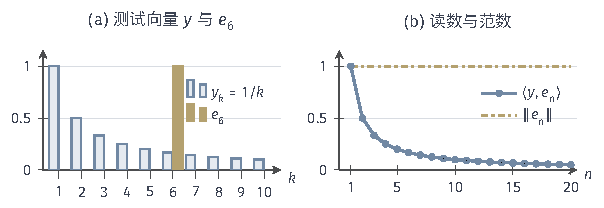
\includegraphics[width=102.3mm]{figures/02-abstract-mathematics/03-function-spaces/tikz/c2-weak-unit-vectors/figure.pdf}
  \caption{$\ell^2$中标准单位向量的弱收敛。(a)~固定读数$y_k=1/k$（浅蓝柱）与$e_6$（黄柱）只在第$6$个坐标重叠；(b)~读数$\langle y,e_n\rangle=1/n$（蓝）趋于零，而范数$\|e_n\|=1$（黄点划线）保持不变。每个固定读数都看到序列趋于零，整体误差却不减小。}
  \label{fig:lfo-weak-unit-vectors}
\end{figure}

\paragraph{振荡的函数}
函数空间中最典型的弱收敛来自振荡。在$L^2(0,2\pi)$中，$\sin(nx)/\sqrt\pi$是标准正交序列，所以$\sin(nx)\rightharpoonup0$。具体地取读数$g=\mathbf 1_{[0,1]}$，得$\int_0^1\sin(nx)\,dx=(1-\cos n)/n\to0$，而$\|\sin(nx)\|_2=\sqrt\pi$保持不变。函数在正负之间越来越快地摆动，任何固定的权重与它相乘再积分时，正负部分都相互抵消。

\paragraph{与测度弱收敛的区别}
第~\ref{sec:measure-sequence-convergence}节也有一个“弱收敛”，但对象和测试都不同。那里变化的是测度$\mu_n$，测试对象是有界连续函数，要求$\int f\,d\mu_n\to\int f\,d\mu$；这里变化的是一个固定线性空间中的元素，测试对象来自该空间的对偶。例如$\delta_{1/n}$作为测度弱收敛到$\delta_0$，但若把它们看成$C([0,1])^*$中的元素，它们之间的全变差距离始终为$2$，在对偶范数下并不收敛；两者的关系要通过第~\ref{sec:lfo-weak-star}节的弱星收敛来说明。两个定义同名，不能只凭名字互换。

\subsection{逐点有界与一致有界}
\label{sec:lfo-uniform-boundedness}

弱收敛只给出逐个读数的信息。我们自然要问：从“每个固定输入上都受控”能否推出某种统一的控制？本小节在Banach空间上给出肯定回答，下一小节再把它用于弱收敛列。

\paragraph{量词能否交换}
设$\{A_\alpha\}_{\alpha\in I}$是$\mathcal B(X,Y)$中的一族算子，并且对每个固定的$x$，$\sup_\alpha\|A_\alpha x\|<\infty$，称为逐点有界。问题是能否推出$\sup_\alpha\|A_\alpha\|<\infty$，即一致有界。前者是“对每个$x$，存在常数$C_x$”，后者是“存在常数$C$，对每个单位$x$”，两者的量词次序不同。

不完备的空间中，答案是否定的。在只有有限项非零的数列组成的空间$c_{00}$上配一致范数，令$L_n(x)=nx_n$。对固定的$x$，$n$超过最后一个非零坐标后$L_n(x)=0$，所以$\sup_n|L_n(x)|<\infty$；可是$\|L_n\|=n$，没有统一上界。下面会看到，完备性正是把逐点有界转为一致有界的关键。

\paragraph{Baire定理}
需要的工具是完备度量空间的一个性质：它不能写成可数个“很瘦”的闭集之并。这一性质称为\term{Baire纲定理}（Baire category theorem）。

\begin{theorem}[Baire纲定理]
\label{thm:lfo-baire}
设$(X,d)$是非空完备度量空间，$F_1,F_2,\ldots$是闭集且$X=\bigcup_kF_k$。则至少有一个$F_k$包含某个开球。
\end{theorem}

\begin{proof}
设每个$F_k$都不含开球，下面构造一个不属于任何$F_k$的点。$F_1$不含开球，所以$X\setminus F_1$是非空开集，可以取闭球$\overline B(x_1,r_1)\subset X\setminus F_1$，$r_1<1$。$F_2$不含开球，所以开球$B(x_1,r_1)$中有点不在$F_2$中，又因$F_2$闭，可取$\overline B(x_2,r_2)\subset B(x_1,r_1)\setminus F_2$，$r_2<1/2$。如此继续，得到嵌套闭球$\overline B(x_k,r_k)$，$r_k<1/k$，且第$k$个球与$F_k$不交。

球心满足$d(x_k,x_m)<r_k$（$m>k$），所以$(x_k)$是Cauchy列。由完备性，$x_k\to x$；每个闭球包含此后的全部球心，故$x\in\overline B(x_k,r_k)$对一切$k$成立，从而$x\notin F_k$对一切$k$成立，与$X=\bigcup_kF_k$矛盾。
\end{proof}

完备性在证明中只用了一次，即保证嵌套球心的极限存在。在$c_{00}$中，同样的嵌套构造可以逼近一个有无穷多非零项的数列，这个极限不在空间中，论证因此失效。下面的\term{一致有界原理}（uniform boundedness principle）把Baire定理用于算子族。

\begin{theorem}[一致有界原理]
\label{thm:lfo-uniform-boundedness}
设$X$是Banach空间，$Y$是赋范空间，$\{A_\alpha\}_{\alpha\in I}\subset\mathcal B(X,Y)$逐点有界，即对每个$x\in X$有$\sup_\alpha\|A_\alpha x\|<\infty$。则$\sup_\alpha\|A_\alpha\|<\infty$。
\end{theorem}

证明按“闭集覆盖—Baire定理给出内点—平移—缩放”的顺序展开。

\begin{proof}
\emph{第一步：层级闭集覆盖空间。}令$F_k=\{x\in X:\sup_\alpha\|A_\alpha x\|\leq k\}$。每个集合$\{x:\|A_\alpha x\|\leq k\}$由连续函数$x\mapsto\|A_\alpha x\|$定义，是闭集，$F_k$是它们的交，也是闭集。逐点有界说明每个$x$属于某个$F_k$，所以$X=\bigcup_kF_k$。

\emph{第二步：某一层含有开球。}$X$完备，由Baire定理，存在$k_0$和开球$B(x_0,r)\subset F_{k_0}$。

\emph{第三步：平移到原点。}对任意$\|z\|<r$，$x_0+z$与$x_0$都在$F_{k_0}$中，于是对每个$\alpha$，
\[
 \|A_\alpha z\|=\|A_\alpha(x_0+z)-A_\alpha x_0\|\leq k_0+k_0=2k_0 .
\]

\emph{第四步：缩放得到统一界。}对任意单位向量$x$及$0<s<r$，$\|sx\|<r$，由上一步$\|A_\alpha x\|=s^{-1}\|A_\alpha(sx)\|\leq2k_0/s$。令$s\to r$，得$\|A_\alpha\|\leq2k_0/r$对一切$\alpha$成立。
\end{proof}

图~\ref{fig:lfo-baire-layers}示意了这个论证。层级集$F_k=kF_1$是对称的闭凸集，一层套一层地覆盖整个空间；Baire定理保证某一层$F_{k_0}$中有一个小球。把这个球平移到原点，两点之差的估计使所有算子在原点附近的小球上一致受控，再用线性缩放推到整个单位球。

\begin{figure}[!htb]
  \centering
  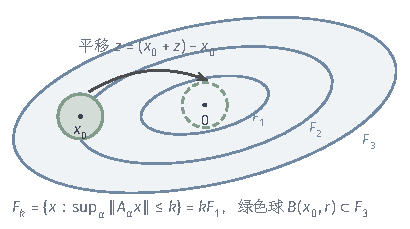
\includegraphics[width=69.3mm]{figures/02-abstract-mathematics/03-function-spaces/tikz/c2-baire-layers/figure.pdf}
  \caption{一致有界原理证明的示意。层级集$F_k=\{x:\sup_\alpha\|A_\alpha x\|\leq k\}$（蓝色嵌套区域）闭、对称且$F_k=kF_1$，它们的并是全空间。Baire定理给出某层（此处$F_3$）中的开球$B(x_0,r)$（绿）；平移到原点后，$z=(x_0+z)-x_0$使$\|z\|<r$时$\|A_\alpha z\|\leq2k_0$，缩放即得$\|A_\alpha\|\leq2k_0/r$。形状只是示意。}
  \label{fig:lfo-baire-layers}
\end{figure}

\paragraph{强收敛的算子列有统一界}
一致有界原理的第一个推论回答了第~\ref{sec:lfo-operator-convergence}节末尾的问题。

\begin{theorem}[Banach--Steinhaus]
\label{thm:lfo-banach-steinhaus}
设$X$是Banach空间，$Y$是赋范空间，$A_n\in\mathcal B(X,Y)$，并且对每个$x$，极限$Ax=\lim_nA_nx$存在。则$\sup_n\|A_n\|<\infty$，$A$是有界线性算子，且$\|A\|\leq\liminf_n\|A_n\|$。
\end{theorem}

\begin{proof}
收敛序列有界，所以$\{A_n\}$逐点有界，由定理~\ref{thm:lfo-uniform-boundedness}一致有界。$A$的线性由极限的线性得到。对单位向量$x$，$\|Ax\|=\lim_n\|A_nx\|\leq\liminf_n\|A_n\|$，对$x$取上确界即得。
\end{proof}

在截断投影的例子中，$\|P_n\|=1$，强极限$I$的范数也是$1$。这个推论说明，Banach空间上的强算子极限不会失去有界性，但它不能改进为算子范数收敛。

\paragraph{同一基础的后续用途}
完备性使量词交换成立，这个基础还会在第~\ref{sec:lfo-open-mapping}节的开映射定理中再用一次，届时直接调用Baire定理，不再重复建立。

\subsection{弱收敛列的范数控制}
\label{sec:lfo-weak-norm}

现在把一致有界原理用于弱收敛列。弱收敛只控制逐个读数，但我们将看到它仍然控制了两件事：序列的范数有统一上界，极限的范数不超过序列范数的下极限。

\begin{theorem}[弱收敛列有界且范数下半连续]
\label{thm:lfo-weak-bounded}
设$X$是赋范空间，$x_n\rightharpoonup x$。则$\sup_n\|x_n\|<\infty$，并且
\begin{equation}
 \|x\|\leq\liminf_{n\to\infty}\|x_n\| .
 \label{eq:lfo-weak-lsc}
\end{equation}
\end{theorem}

\begin{proof}
\emph{有界性。}把每个$x_n$看成对偶空间上的读数：$J_n(L)=L(x_n)$，$L\in X^*$。$J_n$是$X^*$上的线性泛函，它的范数是单位读数在$x_n$上的最大读值，由定理~\ref{thm:lfo-norming-functional}恰好等于$\|x_n\|$。对每个固定的$L$，$J_n(L)=L(x_n)$收敛，因而有界，所以$\{J_n\}$在$X^*$上逐点有界。$X^*$总是Banach空间，由定理~\ref{thm:lfo-uniform-boundedness}得$\sup_n\|x_n\|=\sup_n\|J_n\|<\infty$。

\emph{下半连续。}任取$\|L\|\leq1$，则$|L(x)|=\lim_n|L(x_n)|\leq\liminf_n\|x_n\|$。对$L$取上确界，由式~\eqref{eq:lfo-norm-dual}得式~\eqref{eq:lfo-weak-lsc}。
\end{proof}

证明中用到的完备空间是$X^*$而不是$X$，所以这个结论对不完备的$X$也成立。

\paragraph{不弱收敛的放大序列}
定理给出了一个检验：无界的序列不可能弱收敛。在$\ell^2$中，$\sqrt n\,e_n$的范数趋于无穷，所以它不弱收敛。可以直接找到证据：取$y_k=k^{-3/4}$，$\sum_kk^{-3/2}<\infty$，$y\in\ell^2$，而$\langle y,\sqrt n\,e_n\rangle=n^{1/4}\to\infty$。

\paragraph{范数可以在极限中下降}
式~\eqref{eq:lfo-weak-lsc}可以是严格不等式：$e_n\rightharpoonup0$，$\|0\|=0<1=\liminf\|e_n\|$。弱收敛允许一部分“能量”在极限中消失，例如振荡的$\sin(nx)$弱收敛到零而范数保持$\sqrt\pi$。

\paragraph{Hilbert空间：弱收敛加范数收敛得强收敛}
如果范数没有下降，在Hilbert空间中就能恢复强收敛。设$x_n\rightharpoonup x$且$\|x_n\|\to\|x\|$，展开
\[
 \|x_n-x\|^2=\|x_n\|^2-2\operatorname{Re}\langle x,x_n\rangle+\|x\|^2\longrightarrow\|x\|^2-2\|x\|^2+\|x\|^2=0 .
\]
这里用到了弱收敛$\langle x,x_n\rangle\to\langle x,x\rangle$和内积恒等式。这一步依靠内积，不能作为任意Banach空间的结论。

\paragraph{一般Banach空间中的反例}
在$C([0,1])$中，令$h(t)=\max(0,2t-1)$，$g_n$为支撑在$[0,2/n]$上、在$t=1/n$处取峰值$1$的三角尖峰，$f_n=h+g_n$。$n\geq4$时两部分支撑不交，$\|f_n\|_\infty=1=\|h\|_\infty$。由定理~\ref{thm:lfo-ck-dual}，每个读数都是对某个有限符号测度$\mu$积分；$g_n$一致有界且逐点趋于零，由控制收敛定理$\int g_n\,d\mu\to0$，所以$f_n\rightharpoonup h$。然而$\|f_n-h\|_\infty=\|g_n\|_\infty=1$，不收敛。图~\ref{fig:lfo-weak-norm-drop}画出了这个序列：尖峰贴着左端点越来越窄，不改变最大值，也躲开了每一个固定的测度。

\begin{figure}[!htb]
  \centering
  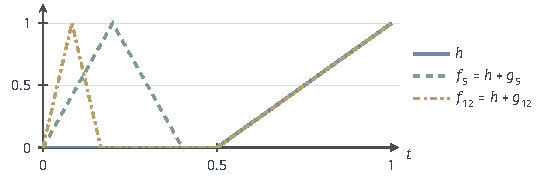
\includegraphics[width=92.8mm]{figures/02-abstract-mathematics/03-function-spaces/tikz/c2-weak-norm-drop/figure.pdf}
  \caption{一致范数下弱收敛加范数收敛不推出强收敛。$h(t)=\max(0,2t-1)$（蓝），$f_n=h+g_n$，其中$g_n$是支撑在$[0,2/n]$、峰值为$1$的尖峰；图中为$n=5$（绿虚线）与$n=12$（黄点划线）。$\|f_n\|_\infty=\|h\|_\infty=1$，$f_n\rightharpoonup h$，但$\|f_n-h\|_\infty=1$。}
  \label{fig:lfo-weak-norm-drop}
\end{figure}

\subsection{Hilbert空间中的弱收敛子列}
\label{sec:lfo-weak-subsequence}

有限维中，有界序列总有收敛子列；无限维中$e_n$说明这对范数收敛不成立。弱收敛的要求更低，本小节证明在Hilbert空间中它恢复了这个性质。

\begin{theorem}[Hilbert空间中的弱子列]
\label{thm:lfo-weak-subsequence}
Hilbert空间中的每个有界序列都有弱收敛的子列。
\end{theorem}

先在可分情形用标准正交基把问题化为系数列，再推广到一般情形。

\begin{proof}
设$\|x_n\|\leq C$。

\emph{第一步：逐个系数抽子列。}先设$H$可分，取标准正交基$(e_k)$，记系数$c_{n,k}=\langle e_k,x_n\rangle$，$|c_{n,k}|\leq C$。有界数列有收敛子列：先从$(x_n)$中抽子列使第$1$个系数收敛，再从中抽子列使第$2$个系数收敛，如此继续。取第$j$个子列的第$j$项组成对角子列$(x_{n_j})$，它从某项起是每个子列的子列，所以对每个$k$，$c_{n_j,k}\to a_k$。

\emph{第二步：极限系数平方可和。}对任意有限的$K$，$\sum_{k\leq K}|a_k|^2=\lim_j\sum_{k\leq K}|c_{n_j,k}|^2\leq C^2$，后一个不等式是Bessel不等式。令$K\to\infty$，$\sum_k|a_k|^2\leq C^2$，所以$x=\sum_ka_ke_k\in H$，$\|x\|\leq C$。

\emph{第三步：对所有方向收敛。}任取$y\in H$及$\varepsilon>0$，取$K$使$\|y-P_Ky\|<\varepsilon$，其中$P_K$是到前$K$个基向量的投影。分解
\[
 \langle y,x_{n_j}-x\rangle=\langle P_Ky,x_{n_j}-x\rangle+\langle y-P_Ky,x_{n_j}-x\rangle .
\]
第一项是有限个系数之差的线性组合，随$j\to\infty$趋于零；第二项不超过$\varepsilon\cdot2C$。所以$\limsup_j|\langle y,x_{n_j}-x\rangle|\leq2C\varepsilon$，由$\varepsilon$任意得$x_{n_j}\rightharpoonup x$。

\emph{第四步：一般Hilbert空间。}令$M$为$\{x_n\}$的闭线性张成。有理系数（复情形为实部虚部都有理）的有限线性组合在$M$中稠密，所以$M$可分，对$M$应用前三步得到子列与$x\in M$，使对一切$y\in M$弱收敛成立。对一般的$y\in H$，写$y=P_My+(y-P_My)$，后者与$M$正交，从而与每个$x_n$及$x$的内积都是零，故$\langle y,x_{n_j}\rangle=\langle P_My,x_{n_j}\rangle\to\langle P_My,x\rangle=\langle y,x\rangle$。
\end{proof}

\paragraph{坐标收敛还不够}
第三步不能省略：逐个系数收敛本身并不等于弱收敛。$x_n=n\,e_n$的每个坐标都最终为零，坐标逐点收敛到零向量，但取$y_k=1/k$，$\langle y,x_n\rangle=1$不趋于零。证明中让有限截断与尾项估计配合的，是序列的统一界$C$；有界性加坐标收敛才推出弱收敛。

\paragraph{弱子列不是范数紧性}
定理只保证弱收敛的子列。单位向量$e_n$本身就弱收敛到零，但没有范数收敛的子列，所以单位球在范数下不紧。弱极限也不必保留序列满足的约束：每个$e_n$都在单位球面$\{\|x\|=1\}$上，弱极限$0$却不在。哪些约束集在弱极限下封闭（例如闭凸集），以及由此得到的极小值存在性，属于优化问题中的存在性讨论，与第~\ref{sec:lfo-finite-observations}节末提到的拟合问题一样留给卷三的优化部分。

\subsection{反射空间的弱紧性（补充）}
\label{sec:lfo-reflexive}

上一小节的证明利用了标准正交基。离开Hilbert空间，有界序列是否仍有弱收敛子列？答案取决于空间与它的二次对偶的关系。

\paragraph{自然嵌入与反射}
每个$x\in X$都给出对偶空间上的一个读数：$(Jx)(L)=L(x)$，$L\in X^*$。$J:X\to X^{**}$线性，由定理~\ref{thm:lfo-norming-functional}，$\|Jx\|=\sup_{\|L\|\leq1}|L(x)|=\|x\|$，所以$J$是保范数的嵌入，称为\term{自然嵌入}（canonical embedding）。若$J$是满射，即$X^{**}$的每个元素都是某个$x$对应的读数，则称$X$为\term{反射空间}（reflexive space）。反射空间必然完备，因为$X^{**}$作为对偶空间是完备的。

有限维空间和Hilbert空间都是反射的：后者用两次Riesz表示即可验证。对$1<p<\infty$，由定理~\ref{thm:lfo-lp-dual}，$(L^p)^*\cong L^q$，$(L^q)^*\cong L^p$，逐层追踪对应关系可以验证合成后正是$J$，所以$L^p$是反射的。第~\ref{sec:lfo-lp-dual}节的端点讨论则表明$\ell^1$不是反射的：它的二次对偶是$(\ell^\infty)^*$，严格大于$\ell^1$。

\begin{theorem}[反射空间的弱紧性]
\label{thm:lfo-reflexive-compact}
设$X$是反射Banach空间。则$X$的闭单位球在弱拓扑下紧，并且$X$中每个有界序列都有弱收敛的子列。
\end{theorem}

\paragraph{为什么要单独陈述序列结论}
弱拓扑一般不能由度量给出，所以第~\ref{sec:metric-compact-sequential-tests}节中“紧等价于序列紧”的结论不能直接套用；从紧性推出序列结论需要另一个定理（Eberlein--Šmulian定理）。对序列结论，可以给一个直接的证明思路：令$Y$为序列的闭线性张成，它可分且反射；由$Y^{**}=J(Y)$可分可推出$Y^*$可分；在$Y^*$的可数稠密集上逐个对角化，得到使每个读数$L(x_{n_j})$都收敛的子列；极限读数是$Y^{**}$的元素，由反射性对应某个$x\in Y$；最后用Hahn--Banach定理把$X^*$中的读数限制到$Y$上，得到$x_{n_j}\rightharpoonup x$。一般证明属于补充。

\paragraph{$L^1$中质量集中的序列}
有界性在非反射空间中不足以保证弱子列。在$L^1(0,1)$中令$f_n=n\mathbf 1_{(0,1/n)}$，$\|f_n\|_1=1$。设某个子列$f_{n_j}\rightharpoonup f\in L^1$。对任意$0<a<1$，取读数$g=\mathbf 1_{(a,1)}\in L^\infty$；当$n_j>1/a$时$\int_a^1f_{n_j}\,dt=0$，所以$\int_a^1f\,dt=0$。对一切$a$成立，相减得$f$在每个区间$(a,b)\subset(0,1)$上积分为零，从而$f=0$几乎处处。但取读数$g\equiv1$，$\int_0^1f_{n_j}\,dt=1$，又得$\int_0^1f\,dt=1$，矛盾。

图~\ref{fig:lfo-escaping-mass}画出了这一列：质量始终为$1$，却向左端点越挤越窄。远离零点的读数（灰色区域）看到的是零，整体积分看到的却是一。极限对象应当是Dirac测度$\delta_0$，它不是$L^1$中的函数，这一列在$L^1$中找不到弱极限。所以第~\ref{sec:lfo-weak-subsequence}节和本小节的结论不能无条件推广到$L^1$或$L^\infty$。

\begin{figure}[!htb]
  \centering
  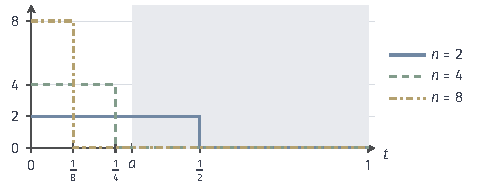
\includegraphics[width=80.8mm]{figures/02-abstract-mathematics/03-function-spaces/tikz/c2-escaping-mass/figure.pdf}
  \caption{$L^1(0,1)$中有界但没有弱收敛子列的序列$f_n=n\mathbf 1_{(0,1/n)}$，图中$n=2,4,8$。每个$f_n$的积分都为$1$；灰色区域是读数$\mathbf 1_{(a,1)}$（$a=0.3$）的支撑，$n>1/a$后在该区域上的积分为零。远离原点的读数迫使候选极限几乎处处为零，整体积分却保持为$1$，二者不能同时满足。}
  \label{fig:lfo-escaping-mass}
\end{figure}

\subsection{对偶空间的弱星紧性（补充）}
\label{sec:lfo-weak-star}

上面的$f_n\,dt$若看成$C([0,1])$上的读数，确实“收敛”到$\delta_0$：对每个连续$u$，$\int_0^1uf_n\,dt\to u(0)$。这提示我们，当变化的对象本身是读数时，可以只用原空间的元素去测试它们。

\begin{definition}[弱星收敛]
\label{def:lfo-weak-star}
设$X$是赋范空间，$L_n,L\in X^*$。若对每个$x\in X$都有$L_n(x)\to L(x)$，则称$L_n$\term{弱星收敛}（weak-star convergence）到$L$，记为$L_n\overset{*}{\rightharpoonup}L$。
\end{definition}

$X^*$本身是Banach空间，它也有自己的弱收敛，测试对象是$X^{**}$的全部元素；弱星收敛只用自然嵌入的像$J(X)\subset X^{**}$测试，要求更少。所以在$X^*$中，弱收敛蕴含弱星收敛，$X$反射时二者一致。

\paragraph{Banach--Alaoglu定理}
弱星收敛的好处是紧性在任何对偶空间中都成立，不需要反射性，这就是\term{Banach--Alaoglu定理}（Banach--Alaoglu theorem）。

\begin{theorem}[Banach--Alaoglu]
\label{thm:lfo-banach-alaoglu}
设$X$是赋范空间。则$X^*$的闭单位球在弱星拓扑下紧。
\end{theorem}

这里的紧性所对应的测试对象是原空间$X$。一般证明把单位球嵌入乘积空间$\prod_{x\in X}[-\|x\|,\|x\|]$，再用Tychonoff定理，属于补充。和反射空间一样，一般的弱星紧性不直接给出序列结论；下面在前对偶$X$可分的条件下给出直接证明。

\begin{theorem}[可分前对偶下的弱星子列]
\label{thm:lfo-weak-star-sequential}
设$X$是可分赋范空间。则$X^*$中每个有界序列都有弱星收敛的子列。
\end{theorem}

\begin{proof}
设$\|L_n\|\leq C$，$\{z_k\}$是$X$的可数稠密子集。对每个$k$，$(L_n(z_k))_n$是有界数列；与定理~\ref{thm:lfo-weak-subsequence}的第一步相同，逐个$k$抽子列再取对角，得到子列$(L_{n_j})$，使$L_{n_j}(z_k)$对每个$k$都收敛。

对一般的$x\in X$及$\varepsilon>0$，取$z_k$使$\|x-z_k\|<\varepsilon$，则
\[
 \begin{aligned}
 |L_{n_i}(x)-L_{n_j}(x)|
 &\leq|L_{n_i}(x-z_k)|+|L_{n_i}(z_k)-L_{n_j}(z_k)|+|L_{n_j}(z_k-x)|\\
 &\leq2C\varepsilon+|L_{n_i}(z_k)-L_{n_j}(z_k)| .
 \end{aligned}
\]
最后一项在$i,j$充分大时小于$\varepsilon$，所以$(L_{n_j}(x))$是Cauchy数列，极限记为$L(x)$。$L$是线性的，且$|L(x)|\leq C\|x\|$，故$L\in X^*$，$L_{n_j}\overset{*}{\rightharpoonup}L$。
\end{proof}

统一的范数界$C$在证明中起了关键作用：它把可数个测试点上的收敛推广到所有测试点。可分性则保证只需对可数个测试点对角化。

\paragraph{$L^\infty$中的振荡}
$L^\infty(0,1)$是可分空间$L^1(0,1)$的对偶，所以其中的有界序列有弱星收敛的子列。取$g_n(t)=\operatorname{sgn}(\sin(2\pi nt))$，它在$2n$个等长小区间上交替取$\pm1$，$\|g_n\|_\infty=1$。对区间的示性函数$f=\mathbf 1_{(a,b)}$，$\int g_nf\,dt$只来自两端不完整的小区间，绝对值不超过$1/n$，趋于零；由线性对阶梯函数成立，再由阶梯函数在$L^1$中稠密及统一界$\|g_n\|_\infty=1$推广到一切$f\in L^1$。所以$g_n\overset{*}{\rightharpoonup}0$，而$\|g_n-g_m\|_\infty$不趋于零，序列不按范数收敛。

同样，$C([0,1])$可分，本小节开头的$f_n\,dt$作为$C([0,1])^*$中的有界序列弱星收敛到$\delta_0$。在$L^1$中找不到的极限，在更大的对偶空间$C([0,1])^*$中以测度的形式出现了。

\paragraph{可分性不能省}
若前对偶不可分，序列结论可以失效。$\ell^\infty$不可分；考虑其对偶中的读数$L_n(x)=x_n$，$\|L_n\|=1$。对任意子列$(L_{n_j})$，取$x\in\ell^\infty$使$x_{n_j}=(-1)^j$（其余坐标为零），则$L_{n_j}(x)=(-1)^j$不收敛。所以这个有界序列没有弱星收敛的子列，尽管Banach--Alaoglu定理仍保证单位球弱星紧。可分性必须写在序列结论之前。

% 第2章第5节：算子的伴随与空间分解（伴随算子、像与核、自伴与正算子及正交投影、条件期望的投影解释）。

\section{算子的伴随与空间分解}
\label{sec:lfo-adjoint}

本节回到Hilbert空间之间的一般算子。前两节说明，Hilbert空间中的每个连续读数都是一个方向；现在用这一点研究算子怎样把输出空间中的测试方向对应回输入空间，并由此回答两个问题：哪些输入方向在输出中完全看不见，哪些输出能被算子的像逼近。自伴与正性进一步刻画同一空间中的方向关系，正交投影和条件期望是最重要的例子。

\subsection{伴随算子}
\label{sec:lfo-adjoint-def}

\paragraph{把输出测试拉回输入}
设$H_1,H_2$是Hilbert空间，$A\in\mathcal B(H_1,H_2)$。固定输出空间中的方向$v\in H_2$，考察读数$u\mapsto\langle v,Au\rangle$：先把输入$u$送到输出空间，再用$v$去测试。它对$u$线性，且$|\langle v,Au\rangle|\leq\|v\|\,\|A\|\,\|u\|$，所以是$H_1$上的有界线性泛函。由Riesz表示定理，存在唯一的$w\in H_1$使$\langle v,Au\rangle=\langle w,u\rangle$对一切$u$成立。这个$w$随$v$而定，记为$A^*v$。

\begin{definition}[伴随算子]
\label{def:lfo-adjoint}
设$A\in\mathcal B(H_1,H_2)$。由
\begin{equation}
 \langle v,Au\rangle_{H_2}=\langle A^*v,u\rangle_{H_1}\qquad(u\in H_1,\ v\in H_2)
 \label{eq:lfo-adjoint}
\end{equation}
确定的映射$A^*:H_2\to H_1$称为$A$的\term{伴随}（adjoint）算子。
\end{definition}

伴随回答的问题是：用输出方向$v$测试$Au$，相当于在输入空间中用哪个方向测试$u$。它把测试方向从输出空间拉回输入空间，并不是从输出恢复输入。下面的移位算子会清楚地显示这一区别。

\begin{theorem}[伴随的基本性质]
\label{thm:lfo-adjoint-properties}
设$A,B\in\mathcal B(H_1,H_2)$，$C\in\mathcal B(H_2,H_3)$，$\alpha\in\mathbb F$。则$A^*\in\mathcal B(H_2,H_1)$，并且
\[
 \begin{aligned}
 &(A+B)^*=A^*+B^*,\quad(\alpha A)^*=\bar\alpha A^*,\quad(CA)^*=A^*C^*,\\
 &A^{**}=A,\quad\|A^*\|=\|A\|,\quad\|A^*A\|=\|A\|^2 .
 \end{aligned}
\]
\end{theorem}

\begin{proof}
\emph{线性。}对$v_1,v_2$及标量$\beta_1,\beta_2$，$\langle A^*(\beta_1v_1+\beta_2v_2),u\rangle=\langle\beta_1v_1+\beta_2v_2,Au\rangle=\bar\beta_1\langle A^*v_1,u\rangle+\bar\beta_2\langle A^*v_2,u\rangle=\langle\beta_1A^*v_1+\beta_2A^*v_2,u\rangle$，由Riesz表示的唯一性即得。和、数乘与复合的公式用同样的方式验证，例如$\langle v,CAu\rangle=\langle C^*v,Au\rangle=\langle A^*C^*v,u\rangle$；数乘中的共轭来自内积对第一个变量共轭线性。

\emph{有界与范数。}由$\|A^*v\|^2=\langle A^*v,A^*v\rangle=\langle v,AA^*v\rangle\leq\|v\|\,\|A\|\,\|A^*v\|$得$\|A^*v\|\leq\|A\|\,\|v\|$，即$\|A^*\|\leq\|A\|$。对$A^*$的伴随求共轭可知$\langle u,A^*v\rangle=\langle Au,v\rangle$，所以$A^{**}=A$，再用一次刚才的不等式得$\|A\|=\|A^{**}\|\leq\|A^*\|$。

\emph{$\|A^*A\|=\|A\|^2$。}一方面$\|A^*A\|\leq\|A^*\|\,\|A\|=\|A\|^2$；另一方面对单位向量$u$，$\|Au\|^2=\langle u,A^*Au\rangle\leq\|A^*A\|$，取上确界得$\|A\|^2\leq\|A^*A\|$。
\end{proof}

\paragraph{矩阵与积分核}
在$\mathbb F^n$与$\mathbb F^m$上配标准内积，矩阵$\bm A$的伴随就是共轭转置$\bm A^{\mathsf H}$，实情形即转置。函数空间中，最常见的例子是积分算子。在$L^2(0,1)$上取$(Vu)(s)=\int_0^su(t)\,dt$，即从$0$累积到$s$。对$v\in L^2(0,1)$，由Fubini定理（定理~\ref{thm:integral-fubini}，被积函数在三角形区域上可积）交换积分次序：
\[
 \langle v,Vu\rangle=\int_0^1\overline{v(s)}\int_0^su(t)\,dt\,ds=\int_0^1\Bigl(\int_t^1\overline{v(s)}\,ds\Bigr)u(t)\,dt ,
\]
所以$(V^*v)(t)=\int_t^1v(s)\,ds$，即从$t$累积到$1$。用$u=v=1$核对：$\langle1,V1\rangle=\int_0^1s\,ds=1/2$，$V^*1=1-t$，$\langle V^*1,1\rangle=\int_0^1(1-t)\,dt=1/2$。一般地，核为$k(s,t)$的积分算子，其伴随的核是$\overline{k(t,s)}$，第~\ref{sec:ose-kernel-symmetry}节将系统讨论。

\paragraph{伴随不是逆}
在$\ell^2$上，右移$S(x_1,x_2,\ldots)=(0,x_1,x_2,\ldots)$的伴随是左移$S^*(y_1,y_2,\ldots)=(y_2,y_3,\ldots)$：逐项核对$\langle y,Sx\rangle=\sum_{k\geq1}\bar y_{k+1}x_k=\langle S^*y,x\rangle$。于是$S^*S=I$，左移撤销了右移；但$SS^*(y_1,y_2,\ldots)=(0,y_2,y_3,\ldots)$，第一个坐标被抹掉了，$SS^*\neq I$。$S$保持长度，不丢失信息，但它的像缺少$e_1$方向，所以$S^*$只是左逆。对一般算子，$A^*$连左逆都不是：零算子的伴随是零算子。

\paragraph{Banach空间中的转置}
没有内积时，仍然可以把输出读数拉回输入。对$A\in\mathcal B(X,Y)$，令$A'L=L\circ A$，$L\in Y^*$，得到\term{转置算子}（transpose operator）$A':Y^*\to X^*$。由定理~\ref{thm:lfo-norming-functional}可以证明$\|A'\|=\|A\|$。转置作用在对偶空间之间；只有在Hilbert空间中借助Riesz对应把读数换成向量，才能把它写成作用在$H_2$与$H_1$之间的伴随$A^*$。

\subsection{像空间与零空间}
\label{sec:lfo-range-kernel}

\paragraph{正交关系}
伴随的定义式~\eqref{eq:lfo-adjoint}把“输出与$Au$正交”翻译成输入空间中的条件。记$\operatorname{Ran}A=\{Au:u\in H_1\}$为像，$\ker A=\{u:Au=0\}$为核。

\begin{theorem}[像与核的正交关系]
\label{thm:lfo-range-kernel}
设$A\in\mathcal B(H_1,H_2)$。则
\begin{equation}
 (\operatorname{Ran}A)^\perp=\ker A^*,\qquad\overline{\operatorname{Ran}A}=(\ker A^*)^\perp ,
 \label{eq:lfo-range-kernel}
\end{equation}
交换$A$与$A^*$的角色，又有$(\operatorname{Ran}A^*)^\perp=\ker A$与$\overline{\operatorname{Ran}A^*}=(\ker A)^\perp$。
\end{theorem}

\begin{proof}
$y\in(\operatorname{Ran}A)^\perp$，当且仅当对一切$u$有$\langle y,Au\rangle=0$，即$\langle A^*y,u\rangle=0$；取$u=A^*y$可知这等价于$A^*y=0$。这证明了第一个等式。

对第二个等式，只需说明线性子空间$M$满足$(M^\perp)^\perp=\overline M$，再取$M=\operatorname{Ran}A$。显然$M\subset(M^\perp)^\perp$，后者是闭集，所以$\overline M\subset(M^\perp)^\perp$。反过来，设$y\in(M^\perp)^\perp$，由第~\ref{sec:fs-projection}节的正交分解$y=P_{\overline M}y+z$，$z\in(\overline M)^\perp=M^\perp$；而$y$与$P_{\overline M}y$都与$z$正交，所以$\|z\|^2=\langle z,y-P_{\overline M}y\rangle=0$，$y\in\overline M$。其余两式把$A$换成$A^*$并用$A^{**}=A$即得。
\end{proof}

由此得到两个空间的正交分解：
\[
 H_1=\ker A\oplus\overline{\operatorname{Ran}A^*},\qquad H_2=\ker A^*\oplus\overline{\operatorname{Ran}A} .
\]
图~\ref{fig:lfo-four-subspaces}把这四个子空间放在一起。$\ker A$中的输入方向在输出中完全看不见，加到任何输入上都不改变输出；$\overline{\operatorname{Ran}A}$是能被输出逼近的方向；$\ker A^*$中的输出方向与一切输出正交，任何输入都到达不了。这是有限维中“四个基本子空间”在Hilbert空间中的形式，区别在于像必须取闭包。

\begin{figure}[!htb]
  \centering
  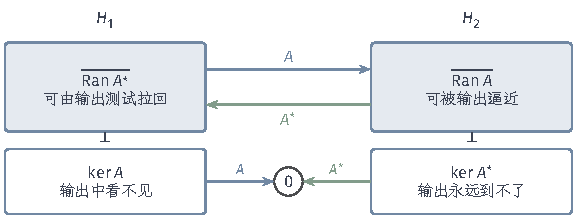
\includegraphics[width=97.7mm]{figures/02-abstract-mathematics/03-function-spaces/tikz/c2-four-subspaces/figure.pdf}
  \caption{伴随与像、核的正交关系。输入空间分解为$H_1=\ker A\oplus\overline{\operatorname{Ran}A^*}$，输出空间分解为$H_2=\ker A^*\oplus\overline{\operatorname{Ran}A}$。$A$把$\ker A$送到零，其余输入的输出都落在$\operatorname{Ran}A$中；$A^*$把$\ker A^*$送到零。无限维中像未必闭合，正交关系只确定像的闭包。}
  \label{fig:lfo-four-subspaces}
\end{figure}

\paragraph{累积算子的像}
以上面的$V$为例。若$V^*v=0$，则$\int_t^1v(s)\,ds=0$对一切$t$成立，于是$v$在每个区间$(t,1)$上积分为零，从而$v=0$几乎处处，$\ker V^*=\{0\}$。由式~\eqref{eq:lfo-range-kernel}，$\operatorname{Ran}V$在$L^2(0,1)$中稠密。但$\operatorname{Ran}V$中的函数都是连续的，阶跃函数$\mathbf 1_{(1/2,1)}$不在其中，所以$\operatorname{Ran}V\neq L^2(0,1)$：像稠密而不闭。

\paragraph{像稠密不闭的数列例子}
在$\ell^2$上令$A(x_n)=(x_n/n)$，即第$n$个坐标乘以$1/n$。它是自伴的（$A^*=A$），单射，所以$\ker A^*=\{0\}$，像在$\ell^2$中稠密。考察$y=(1/n)$，由$\sum_n1/n^2<\infty$知$y\in\ell^2$。若$Ax=y$，逐个坐标比较得$x_n=1$，这个唯一的形式逆像不是平方可和的，所以$y\notin\operatorname{Ran}A$。

截断形式逆像可以看清发生了什么。令$x^{(N)}=(1,\ldots,1,0,0,\ldots)$，前$N$个坐标为$1$。则
\[
 \|Ax^{(N)}-y\|^2=\sum_{n>N}\frac1{n^2}\longrightarrow0,\qquad\|x^{(N)}\|=\sqrt N\longrightarrow\infty .
\]
图~\ref{fig:lfo-dense-range}显示：残差随$N$增大趋于零，说明$y$在像的闭包中；为了取得这些越来越好的近似，输入的范数却无限增大。输出上越来越小的修正需要越来越大的输入，这正是第~\ref{sec:lfo-inverse}节要讨论的不稳定性。

\begin{figure}[!htb]
  \centering
  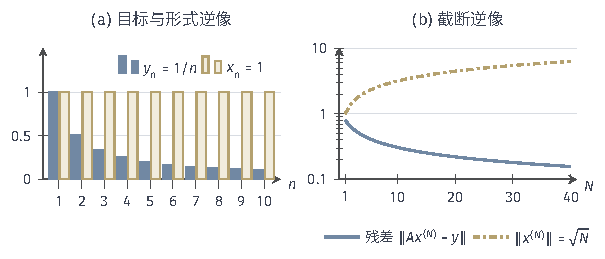
\includegraphics[width=102.5mm]{figures/02-abstract-mathematics/03-function-spaces/tikz/c2-dense-range/figure.pdf}
  \caption{$\ell^2$上$A(x_n)=(x_n/n)$的像稠密而不闭。(a)~目标$y_n=1/n$（蓝）平方可和，但唯一的形式逆像$x_n=1$（黄）不平方可和；(b)~截断逆像$x^{(N)}$的残差$\|Ax^{(N)}-y\|$（蓝）趋于零，范数$\|x^{(N)}\|=\sqrt N$（黄点划线）趋于无穷，纵轴为对数刻度。}
  \label{fig:lfo-dense-range}
\end{figure}

\paragraph{正交条件只确定像的闭包}
这个例子划出了正交关系的边界。$y\perp\ker A^*$只能保证$y$在像的闭包中，不能保证方程$Ax=y$精确可解。只有已经知道$\operatorname{Ran}A$闭合时，才有$\operatorname{Ran}A=(\ker A^*)^\perp$，此时$Ax=y$可解当且仅当$y$与$\ker A^*$正交。第~\ref{chap:operator-spectra-equations}章的Fredholm理论和第一类方程都会反复使用这一边界。

\subsection{自伴、正算子与正交投影}
\label{sec:lfo-self-adjoint}

\paragraph{自伴与正算子}
当输入和输出在同一个Hilbert空间$H$中时，可以比较$A$与$A^*$。若$A=A^*$，即$\langle v,Au\rangle=\langle Av,u\rangle$对一切$u,v$成立，则称$A$为\term{自伴}（self-adjoint）算子。自伴算子的二次型$\langle x,Ax\rangle$总是实数，因为它等于自身的共轭$\langle Ax,x\rangle$。

\begin{definition}[正算子]
\label{def:lfo-positive-operator}
设$A\in\mathcal B(H)$自伴。若$\langle x,Ax\rangle\geq0$对一切$x\in H$成立，则称$A$为\term{正算子}（positive operator），记为$A\geq0$。
\end{definition}

定义中要求先自伴，是因为在实空间中二次型非负并不能推出对称：平面上逆时针旋转$90^\circ$的矩阵满足$\bm x^{\top}\bm A\bm x=0$，却不对称。最基本的正算子是$A^*A$：$\langle x,A^*Ax\rangle=\|Ax\|^2\geq0$。

\paragraph{三种强度的正性}
对自伴算子，下面三个条件依次加强：（i）$\langle x,Ax\rangle\geq0$对一切$x$成立；（ii）$\langle x,Ax\rangle>0$对一切$x\neq0$成立；（iii）存在常数$c>0$，使$\langle x,Ax\rangle\geq c\|x\|^2$对一切$x$成立，此时称$A$具有\term{强制性}（coercivity）。有限维中（ii）与（iii）等价，因为单位球面紧，连续函数在其上取到正的最小值；无限维中不再如此。上一小节的$A(x_n)=(x_n/n)$满足（ii），因为$\langle x,Ax\rangle=\sum_n|x_n|^2/n>0$；但$\langle e_n,Ae_n\rangle=1/n\to0$，没有统一的下界$c$。逐方向严格为正，不能当作统一下界。

统一下界对逆向恢复有直接意义。若$A$自伴且强制，则由Cauchy--Schwarz不等式$c\|x\|^2\leq\langle x,Ax\rangle\leq\|x\|\,\|Ax\|$，得$\|Ax\|\geq c\|x\|$。由此$A$单射；像是闭的，因为若$Ax_n\to y$，则$\|x_n-x_m\|\leq c^{-1}\|Ax_n-Ax_m\|$，$(x_n)$是Cauchy列，极限$x$满足$Ax=y$；又$\ker A^*=\ker A=\{0\}$，由定理~\ref{thm:lfo-range-kernel}像稠密。像既闭又稠密，所以$A$是双射，且$\|A^{-1}\|\leq1/c$。只有逐方向严格正的算子则可能像不闭，正如$(x_n/n)$。

\paragraph{正交投影的算子刻画}
第~\ref{sec:fs-projection}节从最近点问题得到了正交投影$P_M$。现在用算子性质刻画它。

\begin{theorem}[正交投影的刻画]
\label{thm:lfo-orthogonal-projection}
设$P\in\mathcal B(H)$。则$P$是到某个闭子空间的正交投影，当且仅当$P^2=P$且$P^*=P$。此时该子空间为$M=\operatorname{Ran}P$，且$P\geq0$，$\|P\|\leq1$。
\end{theorem}

\begin{proof}
若$P=P_M$，则$P^2=P$是因为$M$中元素的投影是它自己。对任意$x,z$，$\langle z,Px\rangle=\langle Pz+(z-Pz),Px\rangle=\langle Pz,Px\rangle$，因为$z-Pz\perp M$；同理$\langle Pz,x\rangle=\langle Pz,Px\rangle$，所以$P^*=P$。

反过来，设$P^2=P=P^*$。令$M=\operatorname{Ran}P$。由$P^2=P$，$M=\ker(I-P)$，是闭子空间。对任意$x$，$Px\in M$，而$x-Px\in\ker P$；由定理~\ref{thm:lfo-range-kernel}，$\ker P=\ker P^*=(\operatorname{Ran}P)^\perp=M^\perp$。所以$x=Px+(x-Px)$恰是$x$沿$M\oplus M^\perp$的分解，$Px=P_Mx$。最后，$\langle x,Px\rangle=\langle Px,Px\rangle=\|Px\|^2\geq0$，且$\|Px\|^2\leq\|Px\|^2+\|x-Px\|^2=\|x\|^2$。
\end{proof}

只满足$P^2=P$的算子称为投影，它把空间分解为$\operatorname{Ran}P\oplus\ker P$，但两部分不一定正交，这样的投影称为\term{斜投影}（oblique projection）。图~\ref{fig:lfo-projections}(a)中，$P(x_1,x_2)=(x_1+x_2,0)$满足$P^2=P$，像是横轴，核是直线$x_1+x_2=0$。点$\bm x=(0.6,0.9)$被沿核的方向送到$(1.5,0)$，比正交投影$(0.6,0)$离$\bm x$更远。斜投影可以放大长度：$\|P\|=\sqrt2>1$，在方向$(1,1)/\sqrt2$上取到。

\begin{figure}[!htb]
  \centering
  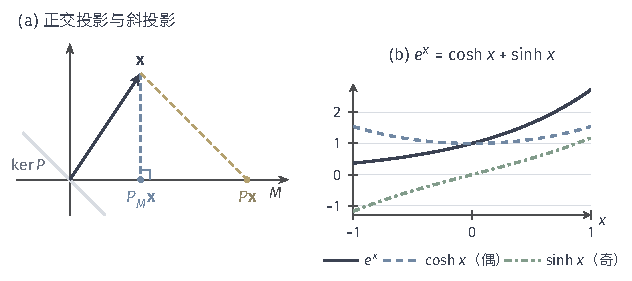
\includegraphics[width=107.0mm]{figures/02-abstract-mathematics/03-function-spaces/tikz/c2-projections/figure.pdf}
  \caption{正交投影与斜投影、偶部分与奇部分。(a)~平面中$\bm x=(0.6,0.9)$到横轴$M$的正交投影为$(0.6,0)$（蓝），残差与$M$垂直；斜投影$P(x_1,x_2)=(x_1+x_2,0)$沿核$x_1+x_2=0$（灰线）把$\bm x$送到$(1.5,0)$（黄），残差不与$M$垂直；(b)~$L^2(-1,1)$中$e^x$分解为偶部分$\cosh x$（蓝虚线）与奇部分$\sinh x$（绿点划线），两部分正交。}
  \label{fig:lfo-projections}
\end{figure}

\paragraph{偶函数投影}
在$L^2(-1,1)$上令
\[
 (Pu)(x)=\frac{u(x)+u(-x)}{2}.
\]
直接验证$P^2=P$。自伴性来自变量替换$x\mapsto-x$保持Lebesgue测度：$\int_{-1}^1\overline{v(x)}u(-x)\,dx=\int_{-1}^1\overline{v(-x)}u(x)\,dx$，于是$\langle v,Pu\rangle=\langle Pv,u\rangle$。由定理~\ref{thm:lfo-orthogonal-projection}，$P$是正交投影，像是偶函数子空间，核是奇函数子空间，两者正交。

以$u(x)=e^x$为例，$Pu=\cosh x$，$(I-P)u=\sinh x$，如图~\ref{fig:lfo-projections}(b)。正交性可以直接核对：$\cosh x\sinh x$是奇函数，在$[-1,1]$上积分为零。勾股恒等式也可以复算：
\[
 \begin{aligned}
 &\|e^x\|^2=\int_{-1}^1e^{2x}\,dx=\sinh2\approx3.627,\\
 &\|\cosh x\|^2=1+\tfrac12\sinh2\approx2.813,\qquad
 \|\sinh x\|^2=\tfrac12\sinh2-1\approx0.813 ,
 \end{aligned}
\]
后两者之和正是前者。若把区间换成不对称的$[-1,2]$，或把测度换成不对称的权重，替换$x\mapsto-x$不再保持内积，同一公式就不再给出正交投影。

\paragraph{有限群平均（补充）}
偶函数投影是对二元群$\{x,-x\}$求平均。一般地，设有限群$G$由保持测度的可逆变换组成，令$(Pu)(x)=|G|^{-1}\sum_{g\in G}u(g(x))$。同样的变量替换说明$P$自伴，群的结构说明$P^2=P$，所以$P$是到$G$不变函数子空间的正交投影。这只是一个空间分解的事实；把数据或模型投影到不变子空间是否改善某个统计任务，需要另外的分析，不能由投影性质直接推出。

\subsection{条件期望的投影解释}
\label{sec:lfo-conditional-expectation}

正交投影最重要的概率实例是条件期望。本小节只补充它的空间解释，所用的条件期望定义与性质先就地写明。

\paragraph{所用的定义与性质}
设$(\Omega,\mathcal F,\mathbb P)$是概率空间，$\mathcal G\subset\mathcal F$是子$\sigma$代数。为避免与空间记号$X$冲突，本小节用$Z$表示随机变量，并只考虑实值情形。对可积的$Z$，\term{条件期望}（conditional expectation）$\mathbb E[Z\mid\mathcal G]$是满足
\begin{equation}
 \mathbb E\bigl[\mathbb E[Z\mid\mathcal G]\,\mathbf 1_A\bigr]=\mathbb E[Z\mathbf 1_A]\qquad(A\in\mathcal G)
 \label{eq:lfo-conditional-expectation}
\end{equation}
的$\mathcal G$可测可积函数，在几乎处处相等的意义下唯一。它的存在性由Radon--Nikodym定理给出，具体做法是取$\mathcal G$上测度$G\mapsto\int_G Z\,d\mathbb P$关于$\mathbb P|_{\mathcal G}$的密度。下面还要用到两个标准性质：条件期望是线性的；条件Jensen不等式给出$(\mathbb E[Z\mid\mathcal G])^2\leq\mathbb E[Z^2\mid\mathcal G]$几乎处处成立。这些性质的系统建立属于第~\ref{part:probability-spaces}部分；离散与有密度情形下的初等版本可参考\BookChapterRef{chap:random-vectors}{卷一“随机向量与联合分布”章}。

\paragraph{$\mathcal G$可测元素组成闭子空间}
令$L^2(\mathcal G)$为$L^2(\Omega,\mathcal F,\mathbb P)$中有$\mathcal G$可测代表的等价类全体，它是线性子空间。它是闭的：设$Z_n\in L^2(\mathcal G)$且$Z_n\to Z$于$L^2$，取各$Z_n$的$\mathcal G$可测代表；由第~\ref{sec:fs-convergence-modes}节，可抽子列$Z_{n_k}\to Z$几乎处处。令$W=\limsup_kZ_{n_k}$（在其取有限值处，其余处取零），它作为$\mathcal G$可测函数的上极限是$\mathcal G$可测的，并且几乎处处等于$Z$，所以$Z\in L^2(\mathcal G)$。这里取上极限而不是直接修改零测集，是为了避免例外零测集本身不属于$\mathcal G$。

\paragraph{条件期望在这个子空间中}
设$Z\in L^2$，记$W=\mathbb E[Z\mid\mathcal G]$。由条件Jensen不等式并对式~\eqref{eq:lfo-conditional-expectation}取$A=\Omega$的形式，
\[
 \mathbb E[W^2]\leq\mathbb E\bigl[\mathbb E[Z^2\mid\mathcal G]\bigr]=\mathbb E[Z^2]<\infty ,
\]
所以$W\in L^2(\mathcal G)$，并且$\|W\|_2\leq\|Z\|_2$。

\paragraph{误差与子空间正交}
接下来验证$Z-W$与$L^2(\mathcal G)$中的每个元素正交。式~\eqref{eq:lfo-conditional-expectation}说明对示性函数$V=\mathbf 1_A$（$A\in\mathcal G$）有$\mathbb E[(Z-W)V]=0$；由线性，对$\mathcal G$可测的简单函数也成立；有界$\mathcal G$可测函数是这类简单函数的一致极限，而$Z-W$可积，所以由控制收敛定理推广到有界的$V$。最后，对一般的$V\in L^2(\mathcal G)$，令截断$V_k=V\mathbf 1_{\{|V|\leq k\}}$，它有界且$\mathcal G$可测；由控制收敛定理$\|V_k-V\|_2\to0$，而内积连续，所以
\[
 \mathbb E[(Z-W)V]=\lim_k\mathbb E[(Z-W)V_k]=0 .
\]

\begin{theorem}[条件期望是正交投影]
\label{thm:lfo-conditional-expectation-projection}
设$Z\in L^2(\Omega,\mathcal F,\mathbb P)$。则$\mathbb E[Z\mid\mathcal G]$是$Z$在闭子空间$L^2(\mathcal G)$上的正交投影。因此$Z\mapsto\mathbb E[Z\mid\mathcal G]$是$L^2$上范数为$1$的自伴正算子，并且
\[
 \mathbb E[(Z-\mathbb E[Z\mid\mathcal G])^2]=\min_{V\in L^2(\mathcal G)}\mathbb E[(Z-V)^2] .
\]
\end{theorem}

\begin{proof}
前面已经说明$W=\mathbb E[Z\mid\mathcal G]\in L^2(\mathcal G)$且$Z-W\perp L^2(\mathcal G)$。由第~\ref{sec:fs-projection}节，满足这两个条件的元素唯一，就是正交投影，并且它是子空间中离$Z$最近的元素。由定理~\ref{thm:lfo-orthogonal-projection}，它是自伴正算子；常数属于$L^2(\mathcal G)$且被保持不变，所以范数等于$1$。
\end{proof}

\paragraph{均方误差的分解}
由第~\ref{sec:fs-projection}节的勾股恒等式，
\[
 \mathbb E[Z^2]=\mathbb E\bigl[(\mathbb E[Z\mid\mathcal G])^2\bigr]+\mathbb E\bigl[(Z-\mathbb E[Z\mid\mathcal G])^2\bigr].
\]
第一项是只用$\mathcal G$中的信息能解释的部分，第二项是这些信息解释不了的残差。定理中的极小性说明，在一切只依赖$\mathcal G$信息的平方可积预测中，条件期望的均方误差最小。

\paragraph{嵌套信息与塔式性质}
若$\mathcal G_1\subset\mathcal G_2$，则$L^2(\mathcal G_1)\subset L^2(\mathcal G_2)$。记$P_1,P_2$为相应的投影，先投影到大的子空间、再投影到小的子空间，等于直接投影到小的子空间：$P_1P_2=P_1$；而小子空间中的元素在大子空间上的投影是它自己：$P_2P_1=P_1$。翻译成条件期望，就是塔式性质
\[
 \mathbb E\bigl[\mathbb E[Z\mid\mathcal G_2]\bigm|\mathcal G_1\bigr]=\mathbb E[Z\mid\mathcal G_1]=\mathbb E\bigl[\mathbb E[Z\mid\mathcal G_1]\bigm|\mathcal G_2\bigr].
\]
$P_1P_2=P_1$的验证只需一行：$P_2Z-Z\perp L^2(\mathcal G_2)\supset L^2(\mathcal G_1)$，所以$P_1(P_2Z)-P_1Z=P_1(P_2Z-Z)=0$。

\paragraph{分块平均的例子}
取$\Omega=[0,1)$，$\mathbb P$为均匀分布，$Z(\omega)=\omega^2$。设$\mathcal G_4$由四个区间$[k/4,(k+1)/4)$生成，$\mathcal G_2$由两半生成。对有限个区间生成的$\sigma$代数，$\mathcal G$可测函数就是在各区间上取常数的函数，式~\eqref{eq:lfo-conditional-expectation}要求条件期望在每个区间上等于$Z$的平均值：
\[
 \mathbb E[Z\mid\mathcal G_4]=4\int_{k/4}^{(k+1)/4}\omega^2\,d\omega=\frac{(k+1)^3-k^3}{48},
\]
即依次为$1/48,7/48,19/48,37/48$；而$\mathbb E[Z\mid\mathcal G_2]$在两半上分别为$1/12$与$7/12$。图~\ref{fig:lfo-conditional-expectation}画出了这两个阶梯函数。粗分块的值正是细分块的值两两再平均，例如$(1/48+7/48)/2=1/12$，这就是塔式性质。

\begin{figure}[!htb]
  \centering
  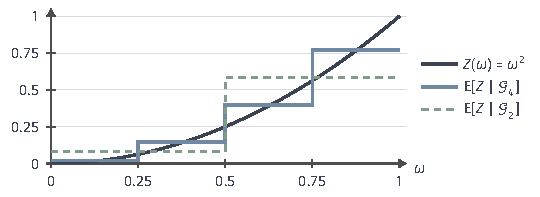
\includegraphics[width=91.4mm]{figures/02-abstract-mathematics/03-function-spaces/tikz/c2-conditional-expectation/figure.pdf}
  \caption{条件期望作为分块平均。$\Omega=[0,1)$上的均匀概率，$Z(\omega)=\omega^2$（黑）。$\mathcal G_4$由四个等长区间生成，$\mathbb E[Z\mid\mathcal G_4]$（蓝）在各区间上取$Z$的平均值$1/48,7/48,19/48,37/48$；$\mathcal G_2$由两半生成，$\mathbb E[Z\mid\mathcal G_2]$（绿虚线）取$1/12,7/12$，恰为细分块值的两两平均。}
  \label{fig:lfo-conditional-expectation}
\end{figure}

均方误差分解也可以复算。$\mathbb E[Z^2]=\int_0^1\omega^4\,d\omega=1/5$。四块时，$\mathbb E[W_4^2]=\frac14\cdot\frac{1+49+361+1369}{48^2}=\frac{1780}{9216}\approx0.1931$，残差约为$0.2-0.1931=0.0069$；两块时，$\mathbb E[W_2^2]=\frac12(\frac1{144}+\frac{49}{144})\approx0.1736$，残差约为$0.0264$。信息越细，子空间越大，投影离$Z$越近。两次投影之间的差$W_4-W_2$与$W_2$正交，$\mathbb E[(W_4-W_2)^2]=\frac{180}{9216}\approx0.0195$，恰好补足$0.1931-0.1736$。

本小节补充的是空间解释，没有重新建立条件期望的存在性。鞅、滤波与状态估计等以条件期望为基础的随机过程问题，可参考\BookChapterRef{chap:random-sequences-and-processes}{卷三“随机序列与随机过程”章}。

% 第2章第6节：逆算子与连续性判别（有界逆与开映射、闭图与图范数）。

\section{逆算子与连续性判别}
\label{sec:lfo-inverse}

由输出恢复输入，要同时满足三个不同的要求：给定的输出确实有原像（存在），原像只有一个（唯一），输出上的小误差只造成输入上的小误差（稳定）。有限维中，方阵可逆就同时满足这三条；无限维中它们会分离。本节先说明在完备性条件下，前两条自动推出第三条，再给出检验连续性的另一种方式。

\subsection{有界逆与开映射}
\label{sec:lfo-open-mapping}

\paragraph{唯一而不稳定}
回到第~\ref{sec:lfo-range-kernel}节的$A(x_n)=(x_n/n)$。它是单射，所以在像$\operatorname{Ran}A$上有唯一的形式逆$A^{-1}(y_n)=(ny_n)$。这个逆映射无界：$A^{-1}e_n=ne_n$，单位输出对应长度为$n$的输入。输出上$e_n/n$大小的误差，会在恢复时变成长度为$1$的输入误差。可解性与唯一性在这里都成立（在像上），稳定性却失败了。

\paragraph{完备空间之间的有界逆}
问题出在哪里？$A$并不是从$\ell^2$到$\ell^2$的双射，它的像只是$\ell^2$中稠密而不闭的子空间，按$\ell^2$范数不完备。下面的\term{有界逆定理}（bounded inverse theorem）说明，只要像是整个Banach空间，这种不稳定就不会发生。

\begin{theorem}[有界逆定理]
\label{thm:lfo-bounded-inverse}
设$X,Y$是Banach空间，$A\in\mathcal B(X,Y)$是双射。则$A^{-1}\in\mathcal B(Y,X)$。
\end{theorem}

定理中的值域是整个$Y$，而且$X,Y$都完备，这些条件都不能省。它说明，在Banach空间之间，有界的线性双射自动是稳定的；可解性加唯一性不足以推出稳定性的情形，一定是某个空间不完备或者像不是全空间。这个定理由下面更一般的\term{开映射定理}（open mapping theorem）推出。

\begin{theorem}[开映射定理]
\label{thm:lfo-open-mapping}
设$X,Y$是Banach空间，$A\in\mathcal B(X,Y)$是满射。则存在$\delta>0$，使$B_Y(0,\delta)\subset A\bigl(B_X(0,1)\bigr)$。等价地，每个$y\in Y$都有原像$x$满足$\|x\|\leq\delta^{-1}\|y\|$。
\end{theorem}

定理的内容是：满射不仅保证每个输出都有原像，还保证能选到一个范数受控的原像。证明分两步，第一步用Baire定理得到“输出球落在输入球的像的闭包中”，第二步用逐步修正残差去掉闭包。

\begin{proof}
记$B_r=B_X(0,r)$。

\emph{第一步：像的闭包含有输出球。}由满射，$Y=\bigcup_kA(B_k)=\bigcup_k\overline{A(B_k)}$。$Y$完备，由Baire定理（定理~\ref{thm:lfo-baire}），某个$\overline{A(B_k)}$包含开球$B_Y(y_0,r)$。对任意$\|y\|<r$，$y_0+y$与$y_0$都在$\overline{A(B_k)}$中，二者之差在$\overline{A(B_k)-A(B_k)}\subset\overline{A(B_{2k})}$中。所以$B_Y(0,r)\subset\overline{A(B_{2k})}$；按线性缩放，令$\eta=r/(2k)$，得
\[
 B_Y(0,\eta)\subset\overline{A(B_1)},\qquad\text{从而}\quad B_Y(0,\eta/2^j)\subset\overline{A(B_{2^{-j}})}\quad(j\geq0).
\]

\emph{第二步：逐步修正残差。}任取$\|y\|<\eta$。由第一步，存在$x_1\in B_1$使$\|y-Ax_1\|<\eta/2$。残差$y_1=y-Ax_1$落在$B_Y(0,\eta/2)$中，于是存在$x_2\in B_{1/2}$使$\|y_1-Ax_2\|<\eta/4$。如此继续，得到$x_k$满足
\[
 \|x_k\|<2^{1-k},\qquad\Bigl\|y-A\sum_{i\leq k}x_i\Bigr\|<\eta/2^k .
\]

\emph{第三步：用输入空间的完备性求和。}$\sum_k\|x_k\|<2$，部分和是$X$中的Cauchy列；$X$完备，所以$x=\sum_kx_k$存在，$\|x\|<2$。由$A$连续，$Ax=\lim_kA\sum_{i\leq k}x_i=y$。这说明$B_Y(0,\eta)\subset A(B_2)$，取$\delta=\eta/2$即得。
\end{proof}

第一步只得到闭包，不能直接说$B_Y(0,\eta)\subset A(B_1)$：闭包中的点只能被像逼近，未必是像。第二步的作用就是把“可以逼近”变成“可以达到”，代价是把输入球的半径从$1$放大到$2$，而这一步必须用到$X$的完备性。图~\ref{fig:lfo-open-mapping}画出了这个修正过程：每一步的修正量减半，输出残差也减半，输入的部分和收敛到真正的原像。

\begin{figure}[!htb]
  \centering
  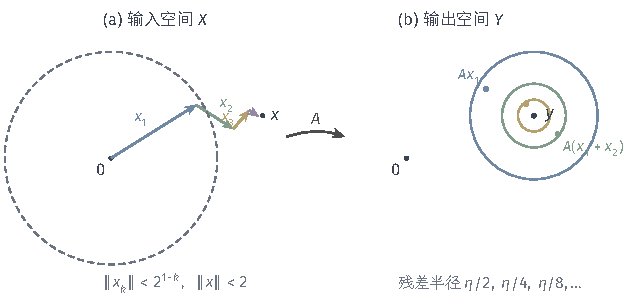
\includegraphics[width=107.4mm]{figures/02-abstract-mathematics/03-function-spaces/tikz/c2-open-mapping/figure.pdf}
  \caption{开映射定理证明中的残差修正（示意）。(b)~输出空间中，第一次近似$Ax_1$落在以$y$为心、半径$\eta/2$的球内（蓝圈），加上修正$x_2$后$A(x_1+x_2)$落入半径$\eta/4$的球（绿圈），依此类推；(a)~输入空间中修正量满足$\|x_k\|<2^{1-k}$，部分和收敛到原像$x$，$\|x\|<2$（虚线圆）。输入空间的完备性保证这一级数有极限。}
  \label{fig:lfo-open-mapping}
\end{figure}

\paragraph{由开映射推出有界逆}
设$A$是Banach空间之间的有界双射。由开映射定理，每个$y$有原像$x$满足$\|x\|\leq\delta^{-1}\|y\|$；单射使这个原像就是$A^{-1}y$，所以$\|A^{-1}y\|\leq\delta^{-1}\|y\|$，$A^{-1}$有界。这证明了定理~\ref{thm:lfo-bounded-inverse}。

\paragraph{等价范数}
有界逆定理的一个直接用途是比较范数。设线性空间$X$在两个范数$\|\cdot\|_a$、$\|\cdot\|_b$下都完备，且$\|x\|_a\leq C\|x\|_b$。则单位映射$I:(X,\|\cdot\|_b)\to(X,\|\cdot\|_a)$是有界双射，其逆也有界，于是存在$C'$使$\|x\|_b\leq C'\|x\|_a$：两个范数等价。若两个完备范数之间只有一个方向的控制，另一个方向的控制会自动出现。

\paragraph{像闭合与下有界}
有界逆定理还给出像闭合的判别。设$X,Y$是Banach空间，$A\in\mathcal B(X,Y)$单射。若$\operatorname{Ran}A$闭，则它是Banach空间，$A:X\to\operatorname{Ran}A$是有界双射，逆有界，于是存在$c>0$使
\begin{equation}
 \|Ax\|\geq c\|x\|\qquad(x\in X),
 \label{eq:lfo-bounded-below}
\end{equation}
这时称$A$\term{下有界}（bounded below）。反过来，若$A$下有界，第~\ref{sec:lfo-self-adjoint}节的论证说明$\operatorname{Ran}A$闭。所以对Banach空间之间的有界单射，像闭合当且仅当下有界。$A(x_n)=(x_n/n)$不满足式~\eqref{eq:lfo-bounded-below}，$\|Ae_n\|=1/n$，它的像也确实不闭。第~\ref{sec:ose-first-kind}节将看到，紧算子在无限维中永远不是下有界的，这正是第一类积分方程不稳定的根源。

\subsection{闭图与图范数（补充）}
\label{sec:lfo-closed-graph}

\paragraph{用极限检验连续性}
直接估计$\|Ax\|\leq C\|x\|$有时很困难。另一种思路是只检验一个较弱的条件：若输入$x_n\to x$，并且输出$Ax_n$也收敛到某个$y$，那么$y$是否必定等于$Ax$？这个条件只涉及输入、输出同时收敛的序列，不要求先证明输出收敛。把它写成几何语言：算子的图
\[
 \mathcal G(A)=\{(x,Ax):x\in D(A)\}\subset X\times Y
\]
在乘积范数$\|(x,y)\|=\|x\|+\|y\|$下是闭集。$X,Y$都完备时，$X\times Y$也是Banach空间。\term{闭图定理}（closed graph theorem）说明，对定义在整个完备空间上的算子，这个较弱的条件已经足够。

\begin{theorem}[闭图定理]
\label{thm:lfo-closed-graph}
设$X,Y$是Banach空间，$A:X\to Y$是定义在整个$X$上的线性算子。则$A$有界当且仅当$\mathcal G(A)$在$X\times Y$中闭。
\end{theorem}

\begin{proof}
若$A$有界，$x_n\to x$推出$Ax_n\to Ax$，所以$Ax_n\to y$时$y=Ax$，图闭。

反过来，设图闭。它是Banach空间$X\times Y$的闭线性子空间，因而本身是Banach空间。第一坐标投影$\pi(x,Ax)=x$是从$\mathcal G(A)$到$X$的有界线性双射（$\|x\|\leq\|(x,Ax)\|$；双射是因为$A$定义在整个$X$上，每个$x$恰好对应图中一点）。由有界逆定理，$\pi^{-1}$有界：存在$C$使$\|x\|+\|Ax\|\leq C\|x\|$，于是$\|Ax\|\leq C\|x\|$。
\end{proof}

\paragraph{处处有定义的对称算子有界}
闭图定理的一个漂亮应用：设$A:H\to H$是定义在整个Hilbert空间上的线性算子，且$\langle v,Au\rangle=\langle Av,u\rangle$对一切$u,v$成立，则$A$有界。只需验证图闭：若$u_n\to u$且$Au_n\to w$，则对任意$v$，
\[
 \langle v,w\rangle=\lim_n\langle v,Au_n\rangle=\lim_n\langle Av,u_n\rangle=\langle Av,u\rangle=\langle v,Au\rangle ,
\]
所以$w=Au$。这里没有估计任何范数，只用了对称性和内积的连续性。反过来说，无界的对称算子（例如适当定义域上的微分算子）不可能定义在整个Hilbert空间上。

\paragraph{定义域只是子空间时}
定理要求$A$定义在整个$X$上。若$A$只定义在子空间$D(A)\subset X$上，图闭合不再意味着有界。回到第~\ref{sec:lfo-boundedness}节的求导$D:D(D)=C^1([0,2\pi])\subset C([0,2\pi])\to C([0,2\pi])$。它的图是闭的：若$u_n\to u$且$u_n'\to v$都按一致范数，则由
\[
 u_n(x)=u_n(0)+\int_0^xu_n'(t)\,dt
\]
两边取极限（一致收敛允许在积分号下取极限）得$u(x)=u(0)+\int_0^xv(t)\,dt$，所以$u\in C^1$且$u'=v$。可是我们已经用$\sin(nx)$说明$D$在一致范数下无界。两者并不矛盾：$D(D)=C^1([0,2\pi])$在一致范数下不完备，闭图定理的条件不满足。图闭合的算子称为\term{闭算子}（closed operator）。

\paragraph{图范数使定义域完备}
对闭算子$A$，在定义域上换用\term{图范数}（graph norm）
\[
 \|u\|_A=\|u\|_X+\|Au\|_Y .
\]
$(D(A),\|\cdot\|_A)$与图$\mathcal G(A)$等距，图闭意味着它完备，而$\|Au\|_Y\leq\|u\|_A$说明$A$在新范数下有界。对求导，图范数正是$\|u\|_\infty+\|u'\|_\infty=\|u\|_{C^1}$，这就回到了第~\ref{sec:lfo-boundedness}节的结论：同一个作用规则，在计入导数的范数下是有界算子。第~\ref{chap:weak-derivatives-sobolev}章的Sobolev范数沿用了同样的思想，用积分范数同时控制函数和它的弱导数。

无界闭算子的谱、由它们生成的算子半群以及相应的演化方程，属于动力系统与轨迹演化问题，可参考\BookChapterRef{chap:action-and-state}{卷三“动力系统”章}。

% 第2章第7节：本章小结。

\section{本章小结}
\label{sec:lfo-summary}

本章围绕一个问题展开：给定一个函数，怎样稳定地变换它或从中读出一个数。第~\ref{sec:lfo-operators}节说明，线性算子是否连续由输入空间、定义域、定义域上的范数和输出空间共同决定，而不由作用公式单独决定。同一个求导规则，在一致范数下无界，在计入导数的范数下有界。算子范数给出一个对全部输入有效的误差界；强算子收敛只对每个输入分别成立，截断投影$P_n\to I$说明二者不能互换。

线性泛函是标量值的算子，它在本章中承担了双重角色。作为读数，它的良定义与连续性要先单独检验：积分读取在$L^p$上总是有界的，点值读取在一致范数下有界，在积分空间中却可能无定义或无界。在Hilbert空间中，有界读数由Riesz表示定理对应到唯一的方向；在$L^p$中对应到$L^q$中的权重，在$C(K)$中对应到测度。作为工具，泛函组成的对偶空间借Hahn--Banach定理区分了任意两个元素，又在弱收敛中充当测试对象，在伴随中把输出测试拉回输入。

弱收敛只控制逐个读数。借助Baire定理和一致有界原理，它仍然控制了序列的范数上界和极限范数的下界；在Hilbert空间和反射空间中，有界序列有弱收敛子列，而$L^1$中的质量集中说明这一结论有边界。可分前对偶的对偶空间中，有界序列有弱星收敛的子列，那些在$L^1$中找不到的极限以测度的形式出现。

伴随揭示了像与核之间的正交关系：$\ker A$是输出中看不见的输入方向，$\ker A^*$的正交补只给出像的闭包。正交投影由幂等与自伴刻画，偶函数投影和条件期望是它在函数空间和概率空间中的两个实例。逆向恢复要分别检查可解、唯一与稳定：Banach空间之间的有界双射有有界逆，但像稠密不闭的单射，例如$(x_n)\mapsto(x_n/n)$，其逆在像上无界。只凭代数上的可逆性，不能判断恢复是否稳定。

第~\ref{chap:operator-spectra-equations}章将限制到能被有限秩算子按算子范数逼近的紧算子，研究它们的谱与奇异值分解，并用本章的伴随、像核关系和有界逆讨论积分方程何时可解、何时稳定。第~\ref{chap:weak-derivatives-sobolev}章用测试函数上的线性泛函定义广义导数，第~\ref{chap:rkhs}章研究点值读数连续的Hilbert空间，并用Riesz表示构造再生核。优化目标、函数拟合与正则化则在本章的空间工具之上另行展开，本章不预先讨论它们的求解方法。


\chapter{算子谱与算子方程}
\label{chap:operator-spectra-equations}

在区间$[-1,1]$上取平均测度$d\mu(z)=dz/2$，用核$K(x,z)=1+xz$把函数$f$变成
\[
  (Tf)(x)=\int_{-1}^{1}(1+xz)f(z)\,d\mu(z)=\int f\,d\mu+x\int zf(z)\,d\mu(z).
\]
无论输入多么复杂，输出总是一个一次函数：这个变换只“看见”$f$的两个矩，其余信息全部丢掉。反过来，若已知输出$g$而要求输入$f$，就会遇到三个问题：$g$必须是什么样子才可能是某个输出？满足$Tf=g$的$f$是否唯一？若$g$带有微小误差，求出的$f$会不会偏得很远？换成$\ell^2$上逐项缩小的变换$A(x_n)=(x_n/n)$，第一个问题仍然存在，后两个问题的答案却变得更微妙：$A$不丢掉任何方向，但沿第$n$个方向把长度压到$1/n$，越往后压得越狠。

上一章为这类问题准备了共同语言：有界算子与算子范数、伴随与像空间的正交关系、弱收敛与一致有界，以及全空间双射的有界逆。但那里的结论对所有有界算子一视同仁，说不出一个变换究竟保留哪些方向、压缩到什么程度。本章把注意力收窄到一类能用有限多个方向统一逼近的算子，并沿着“方向分解—具体实现—逆向求解”的顺序展开。

第~\ref{sec:ose-compact}节定义紧算子：它把有界输入族压成可以抽出收敛子列的输出族，在Hilbert空间中恰好能被有限秩算子按算子范数逼近。第~\ref{sec:ose-spectrum}节研究这些方向的伸缩倍数：先用可逆性定义谱，说明无限维中谱不只由特征值组成；再对紧自伴算子建立正交特征展开，对一般紧算子用输入、输出两组方向写出奇异值分解，并说明截断奇异值给出最佳有限秩逼近。第~\ref{sec:ose-integral-operators}节把这些抽象结论落到积分核上，检查平方可积核为何给出有界、紧的算子，核的对称性又怎样对应伴随与自伴。第~\ref{sec:ose-integral-equations}节回到开头的三个问题，分别研究第二类方程的小范数迭代、紧算子下的Fredholm二择，以及第一类方程中小奇异值怎样放大误差。

全章采用全书的复内积约定：$\langle f,g\rangle$对第一个变量共轭线性、对第二个变量线性，例如$L^2(\mu)$中$\langle f,g\rangle=\int\overline{f}\,g\,d\mu$；伴随满足$\langle v,Au\rangle=\langle A^*v,u\rangle$。主线例子都是实函数，此时共轭不起作用。谱需要复参数才能完整描述，因此第~\ref{sec:ose-spectrum-def}小节在复Hilbert空间中定义谱；实空间中的自伴算子可以按需要复化，不影响本章的结论。

% 第3章第1节：紧算子与有限秩逼近（紧算子与收敛改善、有限秩逼近与算子范数）。

\section{紧算子与有限秩逼近}
\label{sec:ose-compact}

本节固定一个有界线性算子，问它把有界的输入族变成怎样的输出族。有界性只保证输出也有界；在无限维空间中，有界序列未必有收敛子列，所以“有界”还不足以让输出可以被有限多个代表近似。第~\ref{sec:ose-compact-def}小节从有限秩算子出发定义紧性，并说明它怎样把弱收敛的输入变成范数收敛的输出；第~\ref{sec:ose-finite-rank}小节说明紧性在算子范数极限下保持，并在Hilbert空间中把紧算子刻画为有限秩算子的极限。

\subsection{紧算子与收敛改善}
\label{sec:ose-compact-def}

\paragraph{有限秩算子的启发}
先看输出落在有限维空间中的情形。设$X,Y$为赋范空间，有界线性算子$F:X\to Y$的像$\operatorname{Ran}F$是有限维子空间，称$F$为\term{有限秩算子}（finite-rank operator），$\dim\operatorname{Ran}F$称为它的秩。取$\operatorname{Ran}F$的一组基$y_1,\ldots,y_r$，每个输出可以唯一写成$Fx=\sum_{i=1}^{r}\ell_i(x)y_i$，其中系数$\ell_i(x)$随$x$线性变化；由于有限维空间上的范数都等价，$\ell_i$都是有界线性泛函。

若$(x_n)$是$X$中满足$\|x_n\|\leq C$的有界序列，则$\|Fx_n\|\leq\|F\|C$，输出序列落在有限维空间的一个有界集合里。有限维空间中有界序列总有收敛子列（Bolzano–Weierstrass定理），因此$(Fx_n)$有范数收敛的子列。换句话说，有限秩算子把任意有界输入族压成一个“几乎有限”的输出族：只用有限个代表点，就能以任意精度覆盖全部输出。

\paragraph{紧算子的定义}
无限维的输出也可能具有同样的性质。$\ell^2$上的$A(x_n)=(x_n/n)$不是有限秩的，但它把单位球$B=\{x:\|x\|\leq1\}$压进一个越来越扁的集合：输出$y=Ax$满足$|y_n|=|x_n|/n\leq1/n$。图~\ref{fig:ose-compact-ellipse}(a)在前两个坐标张成的平面上画出单位圆及其像，像是半轴为$1$与$1/2$的椭圆；图~\ref{fig:ose-compact-ellipse}(b)显示在所有坐标方向上，像集的“半轴”$1/n$趋于零。从这个集合中取出的任意序列，前有限个坐标可以逐个抽取收敛子列，而尾部坐标被$1/n$统一压小，于是整列也能抽出收敛子列。下面把这一性质取作定义。

\begin{figure}[!htb]
  \centering
  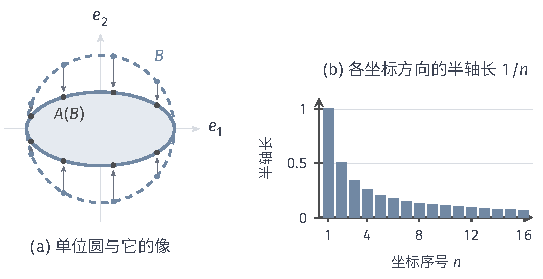
\includegraphics[width=91.9mm]{figures/02-abstract-mathematics/03-function-spaces/tikz/c3-compact-ellipse/figure.pdf}
  \caption{$\ell^2$上的$A(x_n)=(x_n/n)$怎样压缩单位球$B$。(a) 在$e_1,e_2$张成的平面上，虚线单位圆上的点沿箭头映到实线椭圆，椭圆半轴为$1$与$1/2$。(b) 像集$A(B)$的第$n$个坐标不超过$1/n$；越靠后的方向被压得越扁，这正是像集可以被有限个代表点近似覆盖的原因。}
  \label{fig:ose-compact-ellipse}
\end{figure}

\begin{definition}[紧算子]
\label{def:ose-compact-operator}
设$X,Y$为赋范空间，$A:X\to Y$为线性算子。若对$X$中每个有界序列$(x_n)$，输出序列$(Ax_n)$都有在$Y$中按范数收敛的子列，则称$A$为\term{紧算子}（compact operator）。等价地，单位球的像$A(B)$在$Y$中相对紧，即其闭包是紧集。
\end{definition}

紧算子必然有界：若$A$无界，可取单位向量$x_n$使$\|Ax_n\|\geq n$，输出序列的任何子列都无界，不可能收敛。由前面的讨论，每个有界有限秩算子都是紧算子。$A(x_n)=(x_n/n)$的紧性在第~\ref{sec:ose-finite-rank}小节用有限秩逼近给出简洁的证明。

\paragraph{单位算子不紧}
紧性不是每个有界算子都具备的。设$H$为无限维Hilbert空间，取标准正交序列$(e_n)$。对$n\neq m$，由正交性，
\[
  \|e_n-e_m\|^2=\|e_n\|^2+\|e_m\|^2=2 .
\]
单位算子$I$把这个有界序列原样输出，任意两项相距$\sqrt2$，任何子列都不是柯西列，因而没有收敛子列，$I$不是紧算子。同样的序列经过$A(x_n)=(x_n/n)$后变成$Ae_n=e_n/n$，它按范数趋于零。图~\ref{fig:ose-identity-orthonormal}对比了两种输出：左图中三个正交方向两两相距$\sqrt2$，而它们在$A$下的像向原点收拢；右图显示相邻输出的距离在单位算子下恒为$\sqrt2$，在$A$下逐渐趋于零。

\begin{figure}[!htb]
  \centering
  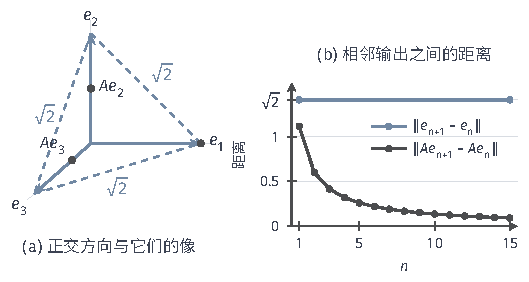
\includegraphics[width=89.6mm]{figures/02-abstract-mathematics/03-function-spaces/tikz/c3-identity-orthonormal/figure.pdf}
  \caption{同一个标准正交序列经过单位算子与经过$A(x_n)=(x_n/n)$的对比。(a) $e_1,e_2,e_3$两两相距$\sqrt2$（虚线），它们在$A$下的像$Ae_1=e_1$、$Ae_2=e_2/2$、$Ae_3=e_3/3$（黑点）向原点收拢。(b) 相邻输出的距离：单位算子下恒为$\sqrt2$，在$A$下等于$\sqrt{1/n^2+1/(n+1)^2}$并趋于零。}
  \label{fig:ose-identity-orthonormal}
\end{figure}

这个例子还提醒我们紧性约束的是什么。由第~\ref{sec:fs-orthogonal-expansion}节，每个$x\in H$都能被它在前$n$个基向量上的截断任意逼近；单独看每个函数，“有限截断”都可行。紧性要求的却是：同一个算子作用于整个有界输入族之后，输出整体可以被有限个代表覆盖。单位算子对每个输入都能截断，对整个单位球却不能，二者的差别正是逐个逼近与统一逼近的差别。

\paragraph{紧算子把弱收敛改善为范数收敛}
第~\ref{sec:lfo-weak-convergence}节已经看到，标准正交序列$e_n\rightharpoonup0$却不按范数收敛。上面的例子中，$Ae_n=e_n/n$按范数收敛到$A0=0$；这不是巧合，紧算子总能把弱收敛的输入变成按范数收敛的输出。

\begin{theorem}[紧算子改善收敛]
\label{thm:ose-compact-weak-strong}
设$X,Y$为赋范空间，$A:X\to Y$为紧算子。若$x_n\rightharpoonup x$，则$\|Ax_n-Ax\|\to0$。
\end{theorem}

\begin{proof}
第一步，说明输入有界、输出弱收敛。由第~\ref{sec:lfo-weak-norm}节，弱收敛序列有界，设$\sup_n\|x_n\|=C<\infty$。对每个$\ell\in Y^*$，复合$\ell\circ A$是$X$上的有界线性泛函，所以$\ell(Ax_n)=(\ell\circ A)(x_n)\to(\ell\circ A)(x)=\ell(Ax)$，即$Ax_n\rightharpoonup Ax$。这一步只用到$A$有界。

第二步，用反证法加上紧性。假设$Ax_n$不按范数收敛到$Ax$，则存在$\varepsilon>0$及子列$(x_{n_k})$，使$\|Ax_{n_k}-Ax\|\geq\varepsilon$对所有$k$成立。子列$(x_{n_k})$仍有界，由紧性可再抽出子列，使相应输出按范数收敛到某个$y\in Y$。

第三步，确认这个极限只能是$Ax$。范数收敛蕴含弱收敛，所以沿这个更细的子列，输出同时弱收敛到$y$和$Ax$。由第~\ref{sec:lfo-hahn-banach}节，连续线性泛函可以区分$Y$中不同的点，故弱极限唯一，$y=Ax$。这与$\|Ax_{n_k}-Ax\|\geq\varepsilon$矛盾。
\end{proof}

证明的分工很清楚：有界性只给出弱收敛被保持，紧性提供范数收敛的子列，弱极限的唯一性再把所有子列的极限钉在同一点。对一般有界算子，第二步不成立：单位算子把$e_n\rightharpoonup0$原样输出，输出仍只是弱收敛。

\subsection{有限秩逼近与算子范数}
\label{sec:ose-finite-rank}

上一小节的例子暗示，紧算子可以看作“有限秩算子的极限”。本小节把这一直觉分成两个方向：先证明紧算子的算子范数极限仍是紧算子，这给出构造紧算子的方法；再在Hilbert空间中证明反方向，即每个紧算子都能由有限秩算子按算子范数逼近。

\paragraph{算子范数极限保持紧性}
证明要用到第~\ref{sec:metric-complete-totally-bounded}节的定理~\ref{thm:metric-compact-complete-tb}：度量空间紧致当且仅当它完备且全有界，全有界指对每个$\varepsilon>0$都能被有限个半径$\varepsilon$的球覆盖。在完备空间$Y$中，全有界集合的闭包仍全有界，又作为闭子集完备，因而是紧集；所以要证像集相对紧，只需证它全有界。

\begin{theorem}[紧算子集合在算子范数下闭]
\label{thm:ose-compact-limit}
设$X$为赋范空间，$Y$为Banach空间，$A_n:X\to Y$都是紧算子，$A\in\mathcal B(X,Y)$且$\|A_n-A\|\to0$，则$A$是紧算子。
\end{theorem}

\begin{proof}
只需证明单位球的像$A(B)$全有界，再用$Y$的完备性得到闭包紧。给定$\varepsilon>0$，先取$n$使$\|A_n-A\|<\varepsilon$。由于$A_n$紧，$A_n(B)$全有界，存在有限个点$y_1,\ldots,y_N\in Y$，使每个$A_nx$（$x\in B$）都满足$\min_i\|A_nx-y_i\|<\varepsilon$。

对任意$x\in B$，选出相应的$y_i$，用三角不等式把误差拆成两段：
\[
  \|Ax-y_i\|\leq\|(A-A_n)x\|+\|A_nx-y_i\|<\|A-A_n\|\,\|x\|+\varepsilon<2\varepsilon .
\]
因此同一组$y_1,\ldots,y_N$是$A(B)$的有限$2\varepsilon$网。$\varepsilon$任意，$A(B)$全有界；$Y$完备，故$\overline{A(B)}$紧，$A$是紧算子。
\end{proof}

关键在于误差界$\|A-A_n\|$对单位球中的所有输入一致成立，于是$A_n$的有限覆盖可以整体搬给$A$。若只知道$A_nx\to Ax$对每个$x$成立，就无法这样搬运；第~\ref{sec:lfo-operator-convergence}节中投影$P_n\to I$逐点成立，而极限$I$恰好不紧。

\begin{example}[对角算子的有限秩逼近]
\label{ex:ose-diagonal-finite-rank}
在$\ell^2$上令$A(x_n)=(x_n/n)$，并令$A_m$只保留前$m$个坐标：$A_mx=(x_1,x_2/2,\ldots,x_m/m,0,0,\ldots)$。$A_m$的像落在前$m$个坐标张成的空间中，是有限秩算子。差$(A-A_m)x$只剩第$m+1$个坐标以后的部分，
\[
  \|(A-A_m)x\|^2=\sum_{n>m}\frac{|x_n|^2}{n^2}\leq\frac{1}{(m+1)^2}\sum_{n>m}|x_n|^2\leq\frac{\|x\|^2}{(m+1)^2},
\]
取$x=e_{m+1}$时等号成立，所以$\|A-A_m\|=1/(m+1)\to0$。由定理~\ref{thm:ose-compact-limit}，$A$是紧算子。
\end{example}

图~\ref{fig:ose-finite-rank-error}把这个误差与单位算子的截断作比较。若用坐标投影$P_m$去逼近单位算子，取$x=e_{m+1}$可知$\|I-P_m\|=1$，无论保留多少坐标，统一误差都不下降；对固定的$x$，误差$\|(I-P_m)x\|$却趋于零，只是趋于零的速度依赖$x$本身。对角算子$A$的截断误差则按$1/(m+1)$对所有单位输入同时下降。

\begin{figure}[!htb]
  \centering
  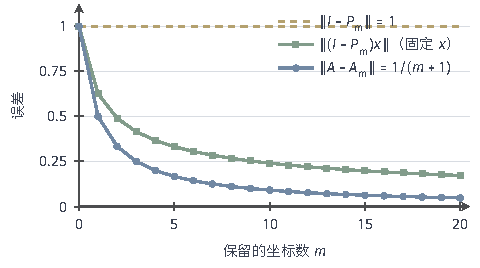
\includegraphics[width=81.2mm]{figures/02-abstract-mathematics/03-function-spaces/tikz/c3-finite-rank-error/figure.pdf}
  \caption{$\ell^2$上三种截断误差随保留坐标数$m$的变化。虚线：单位算子的统一误差$\|I-P_m\|$恒为$1$。方点：固定单位向量$x\propto(1/n)$的误差$\|(I-P_m)x\|$趋于零，但这一速度只属于这个$x$。圆点：紧算子$A(x_n)=(x_n/n)$的统一误差$\|A-A_m\|=1/(m+1)$。}
  \label{fig:ose-finite-rank-error}
\end{figure}

\paragraph{Hilbert空间中紧算子的有限秩逼近}
现在证明反方向。思路是：紧算子的像集可以被有限个点覆盖，这些点张成一个有限维子空间；向这个子空间作正交投影，就得到一个有限秩近似。正交投影的最近点性质（第~\ref{sec:fs-projection}节）保证投影误差不超过到覆盖点的距离。

\begin{theorem}[紧算子的有限秩逼近]
\label{thm:ose-finite-rank-approx}
设$X$为赋范空间，$H$为Hilbert空间，$A:X\to H$为紧算子。则存在有限秩算子$A_n:X\to H$，使$\|A-A_n\|\to0$。
\end{theorem}

\begin{proof}
给定$\varepsilon>0$。由紧性，$A(B)$全有界，取有限个点$y_1,\ldots,y_N$构成$A(B)$的$\varepsilon$网。令$M=\operatorname{span}\{y_1,\ldots,y_N\}$，它是有限维子空间，因而闭；设$P$为到$M$的正交投影，并令$F=PA$。$F$的像含于$M$，且$\|F\|\leq\|P\|\|A\|=\|A\|$，所以$F$是有界有限秩算子。

对任意$x\in B$，选$y_i$使$\|Ax-y_i\|<\varepsilon$。由于$PAx$是$M$中离$Ax$最近的点，而$y_i\in M$，
\[
  \|Ax-Fx\|=\|Ax-PAx\|\leq\|Ax-y_i\|<\varepsilon .
\]
对$x\in B$取上确界得$\|A-F\|\leq\varepsilon$。令$\varepsilon=1/n$，即得所需的有限秩算子列。
\end{proof}

证明中真正用到的是Hilbert空间的正交投影：它把有限覆盖转化为一个有界线性的“取最近点”操作。在一般Banach空间中，有限维子空间上不一定存在范数可控的投影，紧算子能否由有限秩算子按算子范数逼近，取决于空间是否具有所谓的逼近性质；确实存在不具有这一性质的Banach空间，所以本定理不能无条件推广。结合定理~\ref{thm:ose-compact-limit}，在Hilbert空间之间，紧算子恰好是有限秩算子的算子范数极限。后面的积分核逼近（第~\ref{sec:ose-hilbert-schmidt}节）和Fredholm二择的证明（第~\ref{sec:ose-fredholm}节）都会用到这一刻画。

% 第3章第2节：谱与奇异值（谱与特征值、紧自伴算子的谱分解、紧算子的奇异值分解）。

\section{谱与奇异值}
\label{sec:ose-spectrum}

紧算子能被有限秩算子统一逼近，但上一节没有说明应该保留哪些方向、每个方向被放大或压缩多少。有限维中，这个问题由特征值和奇异值回答。本节先用可逆性定义无限维算子的谱，说明它为什么不能只由特征值组成；再在紧自伴条件下建立正交的特征展开；最后对一般紧算子使用输入、输出两组方向，得到奇异值分解及最佳有限秩逼近。

\subsection{谱与特征值}
\label{sec:ose-spectrum-def}

\paragraph{从不可逆性定义谱}
在$n$维空间中，$\bm A-\lambda\bm I$不可逆当且仅当它不是单射，即存在非零向量$\bm v$使$\bm A\bm v=\lambda\bm v$；单射、满射和可逆三者等价，所以“使$\bm A-\lambda\bm I$不可逆的$\lambda$”恰好就是特征值。矩阵的特征值、实对称矩阵的正交对角化与奇异值分解都建立在这一等价关系上，可参考\BookChapterRef{chap:matrix-analysis}{卷一“谱和奇异值”章}。无限维中三者不再等价，必须直接从可逆性出发。

\begin{definition}[谱与预解集]
\label{def:ose-spectrum}
设$H$为复Hilbert空间，$A\in\mathcal B(H)$。若$A-\lambda I$是$H$到$H$的双射，且逆映射$(A-\lambda I)^{-1}$有界，则称$\lambda\in\mathbb C$属于$A$的\term{预解集}（resolvent set），记为$\rho(A)$，并称$(A-\lambda I)^{-1}$为\term{预解算子}（resolvent operator）。预解集的补集$\sigma(A)=\mathbb C\setminus\rho(A)$称为$A$的\term{谱}（spectrum）。若存在非零$u\in H$使$Au=\lambda u$，则称$\lambda$为$A$的\term{特征值}（eigenvalue），$u$为相应的\term{特征向量}（eigenvector）；在函数空间中也常称特征函数。
\end{definition}

由第~\ref{sec:lfo-open-mapping}节的有界逆定理，Banach空间之间的有界线性双射自动有有界逆，所以定义中“逆有界”一项对$A-\lambda I$是全空间双射的情形并不额外增加限制。写出这一项是为了强调：预解参数要求在\emph{整个}$H$上能够稳定地反解$(A-\lambda I)u=g$。特征值使$A-\lambda I$有非零核，当然属于谱；但$A-\lambda I$也可能是单射却不满射，此时只能在像上定义逆映射，这个逆映射还可能没有统一的界。这两种情形都使$\lambda$进入谱，却都不对应非零特征向量。

\paragraph{对角算子的谱}
回到$\ell^2$上的$A(x_n)=(x_n/n)$，逐个检查$\lambda$。若$\lambda=1/k$，则$Ae_k=e_k/k$，所以每个$1/k$都是特征值，特征向量为$e_k$。

再看$\lambda=0$。若$Ax=0$，则每个$x_n/n=0$，所以$A$是单射，$0$不是特征值。但$A$不是满射：第~\ref{sec:lfo-range-kernel}节已经说明，$y=(1/n)\in\ell^2$的唯一形式逆像是常数列$(1,1,\ldots)$，它不平方可和，故$y\notin\operatorname{Ran}A$。即使只在像上考虑逆映射$y\mapsto(ny_n)$，它把单位向量$e_n$送到$ne_n$，范数为$n$，没有统一的界。所以$0\in\sigma(A)$，却不是特征值。

最后取$\lambda$不在集合$S=\{1/n:n\geq1\}\cup\{0\}$中。$S$是闭集（它唯一的聚点$0$已在其中），所以$d=\operatorname{dist}(\lambda,S)>0$。对每个$n$有$|1/n-\lambda|\geq d$，于是方程$(A-\lambda I)x=y$逐坐标解出
\[
  x_n=\frac{y_n}{1/n-\lambda},\qquad \|x\|\leq\frac{1}{d}\|y\| .
\]
这给出全空间上的有界逆，$\lambda\in\rho(A)$。综合三种情形，
\[
  \sigma(A)=\{1/n:n\geq1\}\cup\{0\},\qquad \|(A-\lambda I)^{-1}\|=\frac{1}{\operatorname{dist}(\lambda,\sigma(A))}\quad(\lambda\in\rho(A)).
\]
范数公式中的上界刚刚得到；取$y=e_n$并让$1/n$逼近离$\lambda$最近的谱点，可知上界不能改进。

\begin{figure}[!htb]
  \centering
  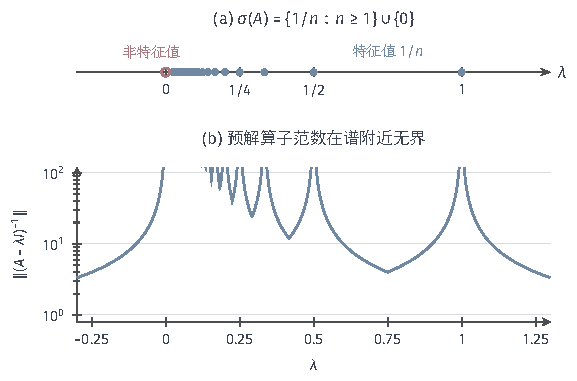
\includegraphics[width=97.8mm]{figures/02-abstract-mathematics/03-function-spaces/tikz/c3-spectrum-resolvent/figure.pdf}
  \caption{$\ell^2$上$A(x_n)=(x_n/n)$的谱。(a) 特征值$1/n$（实心点）向$0$聚集；$0$在谱中但不是特征值（空心点）。(b) 实参数$\lambda$处预解算子的范数$1/\operatorname{dist}(\lambda,\sigma(A))$，纵轴取对数；每个谱点附近范数都无界，在$0$附近这些尖峰挤在一起。}
  \label{fig:ose-spectrum-resolvent}
\end{figure}

图~\ref{fig:ose-spectrum-resolvent}把这三种情形放在一起：特征值是孤立的点，它们聚集到不是特征值的$0$；在任何谱点附近，反解$(A-\lambda I)u=g$的放大倍数都没有上界。三种情形对应三种不同的方向信息：特征值$1/n$对应被精确缩放的方向$e_n$；$0$不对应任何被消去的方向，而是对应一列被压得越来越扁的方向，使像空间稠密却不闭合；远离谱的$\lambda$则让每个方向的缩放倍数$1/n-\lambda$都离零有一段距离。

这一现象对紧算子是普遍的。若$H$无限维而紧算子$A$有有界逆，则$I=A^{-1}A$作为有界算子与紧算子的复合仍是紧算子（有界输入列经$A$后有收敛子列，再经连续的$A^{-1}$仍收敛），与第~\ref{sec:ose-compact-def}小节中单位算子不紧矛盾。所以无限维空间中的紧算子总有$0\in\sigma(A)$，无论$0$是否为特征值。

实Hilbert空间中的算子可以先扩张到复化空间再讨论谱；对下面的自伴算子，特征值都是实数，这样做不会产生新的困难。一般非自伴算子的谱可能含有非实数，其谱分类不在本章展开。

\subsection{紧自伴算子的谱分解}
\label{sec:ose-spectral-theorem}

对角算子的例子中，特征向量$e_n$恰好组成标准正交基，算子就是沿每个基方向乘以一个数。实对称矩阵具有同样的结构：存在由特征向量组成的标准正交基，矩阵在这组基下是实对角矩阵。本小节证明，紧自伴算子在无限维中保留了这一结构：非零特征值至多可数并只能聚集到零，特征方向两两正交，并且与核一起张满整个空间。

\paragraph{紧自伴谱分解的陈述}
自伴算子的定义见第~\ref{sec:lfo-self-adjoint}节：$A\in\mathcal B(H)$满足$A^*=A$，即$\langle v,Au\rangle=\langle Av,u\rangle$对所有$u,v$成立。

\begin{theorem}[紧自伴算子的谱分解]
\label{thm:ose-compact-selfadjoint}
设$H$为实或复Hilbert空间，$A:H\to H$为紧自伴算子。则：
\begin{enumerate}
  \item $A$的特征值都是实数，属于不同特征值的特征向量互相正交；
  \item 每个非零特征值的特征空间有限维；对每个$\delta>0$，满足$|\lambda|\geq\delta$的特征值只有有限个，因此非零特征值至多可数，并且只可能在$0$处聚集；
  \item 存在有限或可数的标准正交序列$(e_j)$及非零实数$\lambda_j$（按重数重复列出，$|\lambda_1|\geq|\lambda_2|\geq\cdots$，序列无限时$\lambda_j\to0$），使$Ae_j=\lambda_je_j$，$(e_j)$的闭张成等于$(\ker A)^\perp$，并且对每个$u\in H$，
  \begin{equation}
    u=u_0+\sum_j\langle e_j,u\rangle e_j,\qquad Au=\sum_j\lambda_j\langle e_j,u\rangle e_j,\qquad u_0\in\ker A,
    \label{eq:ose-spectral-expansion}
  \end{equation}
  两个级数都按$H$的范数收敛。
\end{enumerate}
\end{theorem}

证明的主线是：先说明自伴算子的范数可以由二次型$\langle u,Au\rangle$读出，再用紧性找到使二次型绝对值达到最大的方向，它就是一个特征方向；然后把算子限制到这个方向的正交补上，重复同样的步骤。下面分步完成。

\paragraph{特征值与正交性}
设$Au=\lambda u$，$u\neq0$。由内积对第二变量线性、对第一变量共轭线性，$\langle u,Au\rangle=\lambda\|u\|^2$，$\langle Au,u\rangle=\overline\lambda\|u\|^2$；自伴使两者相等，所以$\lambda=\overline\lambda$为实数。再设$Av=\mu v$，$\mu\neq\lambda$，两者都是实数，于是
\[
  \lambda\langle v,u\rangle=\langle v,Au\rangle=\langle Av,u\rangle=\mu\langle v,u\rangle ,
\]
从而$\langle v,u\rangle=0$。这证明了结论1。

\paragraph{非零特征值的有限性}
设$(e_j)$是一列两两正交的单位特征向量，$Ae_j=\lambda_je_j$且$|\lambda_j|\geq\delta>0$。这种序列可以来自同一个特征空间的标准正交组，也可以来自不同特征值（由结论1自动正交）。对$j\neq k$，
\[
  \|Ae_j-Ae_k\|^2=\|\lambda_je_j-\lambda_ke_k\|^2=|\lambda_j|^2+|\lambda_k|^2\geq2\delta^2 ,
\]
输出列没有柯西子列，与紧性矛盾。所以这种序列只能有限长。取同一特征空间中的标准正交组，即知非零特征空间有限维；取不同特征值的特征向量，即知$|\lambda|\geq\delta$的特征值只有有限个。令$\delta=1,1/2,1/3,\ldots$，非零特征值是可数个有限集合的并，且任何$\delta>0$之外只有有限个，只能在$0$处聚集。这证明了结论2。

\paragraph{二次型给出范数}
设$A$自伴，令$M=\sup_{\|u\|=1}|\langle u,Au\rangle|$。由Cauchy–Schwarz不等式，$|\langle u,Au\rangle|\leq\|A\|$，故$M\leq\|A\|$。反向不等式要从二次型恢复$\|Au\|$。自伴性使$\langle u,Au\rangle=\langle Au,u\rangle=\overline{\langle u,Au\rangle}$为实数，展开可得
\[
  \langle u+v,A(u+v)\rangle-\langle u-v,A(u-v)\rangle=2\langle u,Av\rangle+2\langle v,Au\rangle=4\operatorname{Re}\langle v,Au\rangle ,
\]
其中用到$\langle u,Av\rangle=\langle Au,v\rangle=\overline{\langle v,Au\rangle}$。左边两项各自的绝对值不超过$M\|u\pm v\|^2$，再用平行四边形恒等式$\|u+v\|^2+\|u-v\|^2=2\|u\|^2+2\|v\|^2$，
\[
  4\operatorname{Re}\langle v,Au\rangle\leq M\bigl(\|u+v\|^2+\|u-v\|^2\bigr)=2M\bigl(\|u\|^2+\|v\|^2\bigr).
\]
对单位向量$u$且$Au\neq0$，取$v=Au/\|Au\|$，则$\operatorname{Re}\langle v,Au\rangle=\|Au\|$，上式化为$4\|Au\|\leq4M$。因此$\|A\|\leq M$，两者相等。

\paragraph{紧性给出极值方向}
现设$A\neq0$紧自伴。取单位向量$u_n$使$|\langle u_n,Au_n\rangle|\to\|A\|$。这些二次型都是实数，绝对值趋于$\|A\|>0$，可以抽出子列使它们的符号一致，于是沿该子列$\langle u_n,Au_n\rangle\to\lambda$，其中$\lambda=\|A\|$或$\lambda=-\|A\|$。这里不能预先假定$\lambda$为正：自伴算子的二次型可以取负值，绝对值最大的特征值可能是负的。展开
\[
  \|Au_n-\lambda u_n\|^2=\|Au_n\|^2-2\lambda\langle u_n,Au_n\rangle+\lambda^2\leq2\lambda^2-2\lambda\langle u_n,Au_n\rangle\to0 ,
\]
其中用到$\|Au_n\|\leq\|A\|=|\lambda|$。由紧性，可再抽子列使$Au_n\to w$。于是$\lambda u_n=Au_n-(Au_n-\lambda u_n)\to w$，即$u_n\to e=w/\lambda$，且$\|e\|=1$。由$A$连续，$Ae=\lim Au_n=w=\lambda e$。所以$\pm\|A\|$中至少有一个是特征值，且对应单位特征向量$e$。

\paragraph{逐步分解与核}
记$e_1=e$，$\lambda_1=\lambda$。正交补$H_2=\{e_1\}^\perp$在$A$下不变：若$\langle e_1,v\rangle=0$，则$\langle e_1,Av\rangle=\langle Ae_1,v\rangle=\lambda_1\langle e_1,v\rangle=0$。$A$在$H_2$上的限制仍是紧自伴算子，范数不超过$\|A\|$。若这个限制为零，过程停止；否则对它重复上一段，得到$e_2\perp e_1$及$|\lambda_2|=\|A|_{H_2}\|\leq|\lambda_1|$。依此类推，在$H_k=\{e_1,\ldots,e_{k-1}\}^\perp$上取$e_k$，得到$|\lambda_1|\geq|\lambda_2|\geq\cdots$。若过程不停止，由结论2，$\lambda_k\to0$。

令$M$为$(e_j)$的闭张成。$M^\perp$含于每个$H_k$，所以$A$在$M^\perp$上的限制的范数不超过每个$|\lambda_k|$；过程无限时它趋于零，有限时按停止条件本身为零。因此$A$在$M^\perp$上恒为零，$M^\perp\subseteq\ker A$。反过来，若$Au=0$，则对每个$j$，
\[
  \langle e_j,u\rangle=\frac{1}{\lambda_j}\langle Ae_j,u\rangle=\frac{1}{\lambda_j}\langle e_j,Au\rangle=0 ,
\]
所以$\ker A\subseteq M^\perp$。二者相等，$M=(M^\perp)^\perp=(\ker A)^\perp$。这同时说明每个非零特征值都已出现在$(\lambda_j)$中：属于非零特征值$\mu$的特征向量与$\ker A$正交，因而落在$M$中；若$\mu$不等于任何$\lambda_j$，它就与所有$e_j$正交，只能为零。

\paragraph{展开式}
由第~\ref{sec:fs-orthogonal-expansion}节，$u$在闭子空间$M$上的正交投影为$\sum_j\langle e_j,u\rangle e_j$，级数按范数收敛；余项$u_0$属于$M^\perp=\ker A$。把$A$作用于投影的部分和，由连续性得到$Au=\sum_j\lambda_j\langle e_j,u\rangle e_j$。这就是式~\eqref{eq:ose-spectral-expansion}，证毕。

\paragraph{贯穿例子中的谱分解}
在$L^2([-1,1],\mu)$上，$d\mu=dz/2$，核$K(x,z)=1+xz$给出$(Tf)(x)=\int f\,d\mu+x\int zf\,d\mu$。由$\int1\,d\mu=1$与$\int z^2\,d\mu=\frac12\int_{-1}^{1}z^2\,dz=\frac13$，
\[
  T1=1,\qquad Tx=x\int z^2\,d\mu=\tfrac13x .
\]
单位化得$e_1=1$、$e_2=\sqrt3\,x$（因为$\int3x^2\,d\mu=1$），特征值$\lambda_1=1$、$\lambda_2=1/3$。式~\eqref{eq:ose-spectral-expansion}化为
\[
  Tf=\langle e_1,f\rangle e_1+\tfrac13\langle e_2,f\rangle e_2 ,
\]
与$1,x$都正交的函数组成$\ker T$，它是无限维的。第~\ref{sec:ose-kernels}小节将在积分核的语言下再看这个例子。

把核换成$1-6xz$，常数方向不变，线性方向变为$T x=-6x\int z^2\,d\mu=-2x$，特征值$-2$的绝对值最大。图~\ref{fig:ose-spectral-stretch}(b)在$e_1,e_2$的系数平面上画出单位圆的像：沿$e_1$方向不变，沿$e_2$方向拉长两倍并翻转，点$p$被送到$e_2$坐标反号的$Tp$。若只寻找正的最大特征值，就会漏掉这个主导方向。图~\ref{fig:ose-spectral-stretch}(a)则显示$\ell^2$对角算子的情形：$u$的每个系数$\langle e_j,u\rangle$被乘以$\lambda_j=1/j$，后面的方向被压得更小。

\begin{figure}[!htb]
  \centering
  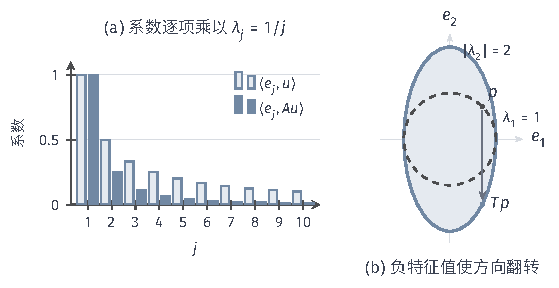
\includegraphics[width=94.6mm]{figures/02-abstract-mathematics/03-function-spaces/tikz/c3-spectral-stretch/figure.pdf}
  \caption{紧自伴算子沿特征方向逐个伸缩。(a) $\ell^2$上$A=\operatorname{diag}(1/j)$，浅色条为$u$的系数$\langle e_j,u\rangle=1/j$，深色条为$Au$的系数$1/j^2$。(b) $L^2([-1,1],dz/2)$上核$1-6xz$的积分算子，在$e_1=1$、$e_2=\sqrt3x$的系数平面上把虚线单位圆映为实线椭圆：$e_1$方向乘$1$，$e_2$方向乘$-2$。与$1,x$正交的方向全部被映为零，图中未画出。}
  \label{fig:ose-spectral-stretch}
\end{figure}

\paragraph{展开的收敛方式}
式~\eqref{eq:ose-spectral-expansion}中的级数按Hilbert空间的范数收敛。对$L^2(\mu)$中的函数，这意味着平方积分误差趋于零，并不意味着在每个点或一致地收敛；$L^2$的元素本来就是几乎处处等价类，单独谈某一点的值没有意义。若要把特征展开写成核函数$K(x,z)=\sum_j\lambda_je_j(x)\overline{e_j(z)}$的逐点甚至一致收敛的级数，需要核连续、半正定等额外条件，这是第~\ref{sec:rkhs-mercer}节Mercer定理讨论的内容。

\subsection{紧算子的奇异值分解}
\label{sec:ose-svd}

非自伴算子不一定有足够多的特征向量，输入与输出甚至可以位于不同的空间。有限维中，矩阵的奇异值分解用输入、输出各一组标准正交方向解决这个问题。对紧算子，同样的构造可以通过正紧自伴算子$A^*A$完成。

\paragraph{从$A^*A$构造两组方向}
设$H_1,H_2$为Hilbert空间，$A:H_1\to H_2$为紧算子。$A^*A:H_1\to H_1$是紧算子：有界输入列经$A$后有收敛子列，再经连续的$A^*$仍收敛。它也是自伴的，且
\[
  \langle x,A^*Ax\rangle=\langle Ax,Ax\rangle=\|Ax\|^2\geq0 ,
\]
所以它的特征值都非负，并且$A^*Ax=0$当且仅当$Ax=0$，即$\ker(A^*A)=\ker A$。

对$A^*A$应用定理~\ref{thm:ose-compact-selfadjoint}，得到标准正交的特征向量$v_j$与正特征值$s_j$，按递减顺序排列。令$\sigma_j=\sqrt{s_j}$，再令$u_j=Av_j/\sigma_j$。这组输出方向也是标准正交的：
\[
  \langle u_j,u_k\rangle=\frac{\langle Av_j,Av_k\rangle}{\sigma_j\sigma_k}=\frac{\langle v_j,A^*Av_k\rangle}{\sigma_j\sigma_k}=\frac{\sigma_k^2\langle v_j,v_k\rangle}{\sigma_j\sigma_k}=\delta_{j,k} .
\]
此外$A^*u_j=A^*Av_j/\sigma_j=\sigma_jv_j$，所以$A$把$v_j$送到$\sigma_ju_j$，$A^*$把$u_j$送回$\sigma_jv_j$。

\begin{theorem}[紧算子的奇异值分解]
\label{thm:ose-svd}
设$A:H_1\to H_2$为紧算子，$\sigma_1\geq\sigma_2\geq\cdots>0$及标准正交序列$(v_j)\subset H_1$、$(u_j)\subset H_2$如上构造。则对每个$x\in H_1$、$y\in H_2$，
\begin{equation}
  Ax=\sum_j\sigma_j\langle v_j,x\rangle u_j,\qquad A^*y=\sum_j\sigma_j\langle u_j,y\rangle v_j ,
  \label{eq:ose-svd}
\end{equation}
级数按范数收敛。$(v_j)$的闭张成为$(\ker A)^\perp$，$(u_j)$的闭张成为$\overline{\operatorname{Ran}A}=(\ker A^*)^\perp$。序列无限时$\sigma_j\to0$。
\end{theorem}

\begin{proof}
由定理~\ref{thm:ose-compact-selfadjoint}，$(v_j)$的闭张成为$(\ker A^*A)^\perp=(\ker A)^\perp$，任意$x$可写成$x=x_0+\sum_j\langle v_j,x\rangle v_j$，$x_0\in\ker A$。把$A$作用于部分和并取极限，得$Ax=\sum_j\langle v_j,x\rangle Av_j=\sum_j\sigma_j\langle v_j,x\rangle u_j$。由这一展开，每个$Ax$都落在$(u_j)$的闭张成中；反之每个$u_j=A(v_j/\sigma_j)$属于$\operatorname{Ran}A$。所以$(u_j)$的闭张成等于$\overline{\operatorname{Ran}A}$，再由第~\ref{sec:lfo-range-kernel}节得它等于$(\ker A^*)^\perp$。关于$A^*$的展开，对任意$x$有
\[
  \langle x,A^*y\rangle=\langle Ax,y\rangle=\sum_j\sigma_j\overline{\langle v_j,x\rangle}\langle u_j,y\rangle=\Bigl\langle x,\sum_j\sigma_j\langle u_j,y\rangle v_j\Bigr\rangle ,
\]
右端级数因系数平方可和而收敛，两边对所有$x$相等，故展开成立。$\sigma_j\to0$来自$s_j\to0$。
\end{proof}

数$\sigma_j$称为$A$的\term{奇异值}（singular value），$v_j$与$u_j$分别称为\term{右奇异向量}（right singular vector）与\term{左奇异向量}（left singular vector）。展开式~\eqref{eq:ose-svd}说明$A$的作用分三步：读出输入在$v_j$方向上的系数，乘以$\sigma_j$，再放到输出方向$u_j$上。输入中的$\ker A$完全看不见；输出中的$\ker A^*$则是永远到达不了的方向。两组方向一般属于不同的空间，即使$H_1=H_2$，$u_j$也未必等于$v_j$；只有正自伴算子才使两组方向重合、奇异值等于特征值。

\begin{example}[积分算子的奇异值分解]
\label{ex:ose-volterra-svd}
在$L^2(0,1)$上（Lebesgue测度），令$(Vf)(x)=\int_0^xf(t)\,dt$。它是核$\mathbf 1_{\{t<x\}}$的积分算子；这个核在$[0,1]^2$上平方可积，第~\ref{sec:ose-hilbert-schmidt}小节将证明这样的积分算子是紧算子，这里先承认这一点。由Fubini定理交换积分次序，伴随为$(V^*g)(t)=\int_t^1g(x)\,dx$，于是
\[
  (V^*Vf)(t)=\int_t^1\Bigl(\int_0^xf(s)\,ds\Bigr)dx .
\]

设$V^*Vf=sf$，$s>0$。右端是连续函数，所以$f=s^{-1}V^*Vf$连续；于是$Vf$连续可微，$V^*Vf$二次连续可微，$f$也二次连续可微。对$t$求导两次得$(V^*Vf)'=-Vf$、$(V^*Vf)''=-f$，因此$sf''=-f$；又由表达式直接读出$(V^*Vf)'(0)=0$、$(V^*Vf)(1)=0$，故$f'(0)=0$、$f(1)=0$。满足这些条件的非零解为$f(t)=c\cos(\omega t)$，其中$\omega=s^{-1/2}$且$\cos\omega=0$，即$\omega_k=(k-\tfrac12)\pi$，$k=1,2,\ldots$。

$V$是单射：若$\int_0^xf=0$对所有$x$成立，则$E\mapsto\int_Ef^+$与$E\mapsto\int_Ef^-$在所有区间上相等，由定理~\ref{thm:measure-pi-lambda-uniqueness}在全部Borel集上相等，取$E=\{f>0\}$即知$f\leq0$几乎处处，同理$f\geq0$几乎处处。于是$\ker V^*V=\ker V=\{0\}$，由定理~\ref{thm:ose-compact-selfadjoint}，$V^*V$的特征向量张满整个$L^2(0,1)$。由此得到
\[
  \sigma_k=\frac{1}{(k-\frac12)\pi}=\frac{2}{(2k-1)\pi},\qquad
  \begin{aligned}
    v_k(t)&=\sqrt2\cos\bigl((k-\tfrac12)\pi t\bigr),\\
    u_k(x)&=\sqrt2\sin\bigl((k-\tfrac12)\pi x\bigr),
  \end{aligned}
\]
其中$u_k=Vv_k/\sigma_k$可直接积分验证。前几个奇异值约为$0.637$、$0.212$、$0.127$、$0.091$，按$1/k$的速度衰减。
\end{example}

\paragraph{截断奇异值与最佳有限秩逼近}
奇异值分解直接给出有限秩逼近：只保留前$m$项，
\[
  A_mx=\sum_{j\leq m}\sigma_j\langle v_j,x\rangle u_j .
\]
下面的定理说明这个截断的误差恰为下一个奇异值，并且没有任何秩不超过$m$的算子做得更好。若正奇异值只有有限个，约定用尽之后的$\sigma_j=0$。

\begin{theorem}[截断奇异值分解的最优性]
\label{thm:ose-svd-truncation}
在定理~\ref{thm:ose-svd}的条件下，$\|A-A_m\|=\sigma_{m+1}$；对每个秩不超过$m$的有界算子$F:H_1\to H_2$，都有$\|A-F\|\geq\sigma_{m+1}$。
\end{theorem}

\begin{proof}
第一步，计算截断误差。由式~\eqref{eq:ose-svd}及$(u_j)$的正交性，
\[
  \|(A-A_m)x\|^2=\sum_{j>m}\sigma_j^2|\langle v_j,x\rangle|^2\leq\sigma_{m+1}^2\sum_{j>m}|\langle v_j,x\rangle|^2\leq\sigma_{m+1}^2\|x\|^2 ,
\]
其中最后一步是Bessel不等式。取$x=v_{m+1}$时等号成立（若$\sigma_{m+1}=0$，结论已由上式得到），所以$\|A-A_m\|=\sigma_{m+1}$。

第二步，证明下界。不妨设$\sigma_{m+1}>0$。令$W=\operatorname{span}\{v_1,\ldots,v_{m+1}\}$，它是$m+1$维的。$F$在$W$上的限制把$W$映入维数不超过$m$的$\operatorname{Ran}F$，由线性代数的维数公式，存在单位向量$x\in W$使$Fx=0$。写$x=\sum_{j\leq m+1}c_jv_j$，$\sum_j|c_j|^2=1$，则
\[
  \|(A-F)x\|^2=\|Ax\|^2=\sum_{j\leq m+1}\sigma_j^2|c_j|^2\geq\sigma_{m+1}^2 .
\]
因此$\|A-F\|\geq\sigma_{m+1}$。
\end{proof}

\begin{figure}[!htb]
  \centering
  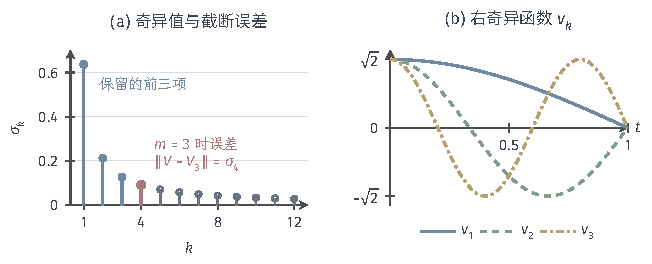
\includegraphics[width=110.3mm]{figures/02-abstract-mathematics/03-function-spaces/tikz/c3-svd-decay/figure.pdf}
  \caption{积分算子$(Vf)(x)=\int_0^xf$在$L^2(0,1)$上的奇异值分解。(a) 奇异值$\sigma_k=2/((2k-1)\pi)$；保留前三项（蓝色）时，算子范数误差等于第四个奇异值$\sigma_4\approx0.091$（红色），后面的奇异值（空心）全部被舍去。(b) 前三个右奇异函数$v_k(t)=\sqrt2\cos((k-\frac12)\pi t)$，序号越大振荡越快。}
  \label{fig:ose-svd-decay}
\end{figure}

图~\ref{fig:ose-svd-decay}在积分算子$V$上展示这一结论。保留前三项时误差为$\sigma_4\approx0.091$；奇异值衰减越快，同样秩的截断误差越小。右图显示，奇异值越小的方向振荡越快：$V$是积分，它把快速振荡的输入平均掉，输出的幅度只剩$1/\omega_k$倍。对比$\ell^2$上的$A(x_n)=(x_n/n)$，它是正自伴算子，奇异值就是特征值$1/n$，左右奇异向量都是$e_n$，例~\ref{ex:ose-diagonal-finite-rank}中的截断正是截断奇异值分解。

小奇异值对正向逼近是好消息：它们可以被舍去而误差很小。对反向求解却是坏消息：要从输出恢复输入，必须把这些方向上的系数除以$\sigma_j$。这一障碍留到第~\ref{sec:ose-first-kind}小节处理。

% 第3章第3节：积分算子（积分核与函数变换、平方可积核与紧性、核的对称性与算子伴随）。

\section{积分算子}
\label{sec:ose-integral-operators}

前两节的结论针对抽象的紧算子。本节用积分核具体地实现它们：先检查积分公式在什么意义下定义一个算子，再给出有界与紧所需的平方可积条件，最后把核的对称性与伴随、自伴联系起来。贯穿全节的一个提醒是：同一个核公式只有连同输入空间、输出空间和测度一起给出，才确定一个算子。

\subsection{积分核与函数变换}
\label{sec:ose-kernels}

\paragraph{积分公式的三个待查问题}
设$(X,\mu)$与$(Y,\nu)$为$\sigma$有限测度空间，$K:Y\times X\to\mathbb F$关于乘积$\sigma$代数可测。对$X$上的函数$f$，形式地定义
\begin{equation}
  (Tf)(y)=\int_XK(y,x)f(x)\,d\mu(x),\qquad y\in Y .
  \label{eq:ose-integral-operator}
\end{equation}
称$K$为\term{积分核}（integral kernel），$T$为以$K$为核的\term{积分算子}（integral operator）。核的第一个变量是输出位置，第二个变量是输入位置：固定$y$时，$K(y,\cdot)$是对输入$f$加权平均所用的权重。

公式~\eqref{eq:ose-integral-operator}本身只是一个形式表达。要让它确实定义一个算子$T:L^p(\mu)\to L^q(\nu)$，需要依次检查三件事：对哪些$y$，积分绝对收敛；把这些积分值拼成的函数$y\mapsto(Tf)(y)$是否可测；它是否属于目标空间$L^q(\nu)$。由于输入$f$只是几乎处处等价类，积分值不受$f$在零测集上改动的影响；输出也只能确定到$\nu$几乎处处，即$Tf$同样是一个等价类。第~\ref{sec:ose-hilbert-schmidt}小节将在平方可积的条件下完成这三项检查。

\paragraph{三种“核”的区别}
“核”这个词在本书中有几种不同的用法，不能因为名称相同就沿用相同的条件。第~\ref{sec:cond-kernels}节的概率核为每个输入点指定一个概率测度，要求非负且总质量为一，表示随机转移；第~\ref{sec:rkhs-kernel-properties}节的正定核要求对所有有限点集形成的Gram矩阵半正定，用来构造点值读取连续的函数空间。本节的积分核只是一个标量函数，可以取负值，不要求归一化，也不要求对称或正定；它通过积分把一个函数变成另一个函数。

\paragraph{贯穿例子：核如何选择方向}
在$X=Y=[-1,1]$上取$d\mu(z)=dz/2$与$K(x,z)=1+xz$。核可以拆成两个分离变量的乘积之和：$K(x,z)=1\cdot1+x\cdot z$。代入公式~\eqref{eq:ose-integral-operator}，
\[
  (Tf)(x)=\int_{-1}^{1}f\,d\mu+x\int_{-1}^{1}zf(z)\,d\mu(z) .
\]
输出总是一次函数，系数分别是输入的零阶矩与一阶矩。取$f=1+x$，由$\int(1+z)\,d\mu=1$与$\int z(1+z)\,d\mu=\int z^2\,d\mu=1/3$，得$Tf=1+x/3$：常数部分原样保留，斜率被压到原来的三分之一。再取$q(x)=x^2-1/3$，它的零阶矩$\int z^2\,d\mu-1/3=0$，一阶矩是奇函数的积分，也为零，所以$Tq=0$。

\begin{figure}[!htb]
  \centering
  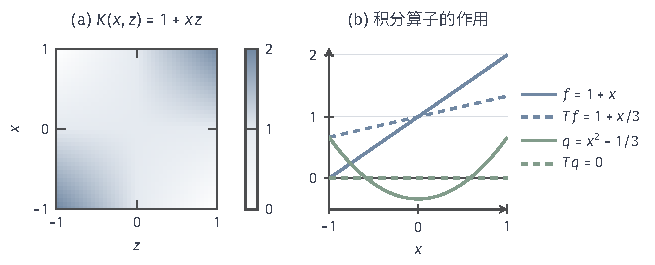
\includegraphics[width=110.9mm]{figures/02-abstract-mathematics/03-function-spaces/tikz/c3-kernel-action/figure.pdf}
  \caption{核$K(x,z)=1+xz$及其积分算子在$L^2([-1,1],dz/2)$上的作用。(a) 核的热图，颜色越深取值越大；沿对角方向$xz>0$时权重大于$1$。(b) $f=1+x$被映为$Tf=1+x/3$，常数方向保留、线性方向乘$1/3$；与$1,x$都正交的$q=x^2-1/3$被映为零。}
  \label{fig:ose-kernel-action}
\end{figure}

图~\ref{fig:ose-kernel-action}把核与作用放在一起。左图中的权重随$x,z$同号或异号而增减，正是这种结构使输出只记住输入的“平均”和“倾斜”；右图中，$q$虽然不是零函数，却与两个被记住的方向都正交，因而完全被消去。用第~\ref{sec:ose-spectral-theorem}小节的语言，$1$与$\sqrt3x$是特征值$1$与$1/3$的特征函数，$q$属于无限维的核空间。由于输出落在二维空间$\operatorname{span}\{1,x\}$中，$T$是秩为$2$的有限秩算子；一般地，$K(y,x)=\sum_{i=1}^r\varphi_i(y)\psi_i(x)$这类分离变量的有限和总给出秩不超过$r$的积分算子。

\paragraph{测度是算子的一部分}
保持核公式不变，把测度换成Lebesgue测度$dz$，两个矩都加倍，算子变成
\[
  (\tilde Tf)(x)=\int_{-1}^{1}(1+xz)f(z)\,dz=2\int f\,d\mu+2x\int zf\,d\mu ,
\]
于是$\tilde T(1+x)=2+2x/3$，特征值变为$2$与$2/3$，单位特征函数也随新内积重新归一化。同一个核在不同测度下给出不同的算子，谱也随之改变；讨论积分算子的谱时，必须同时报告核和测度。

\subsection{平方可积核与紧性}
\label{sec:ose-hilbert-schmidt}

现在给出一个容易检查的条件，使公式~\eqref{eq:ose-integral-operator}定义$L^2(\mu)$到$L^2(\nu)$的有界算子，并进一步是紧算子。下面用到的乘积测度与一般测度空间上的Tonelli、Fubini定理见本卷第~\ref{sec:integral-iterated}节（定理~\ref{thm:analysis-tonelli-fubini}与定理~\ref{thm:integral-fubini}）。

\paragraph{有界性}
逐点看，$(Tf)(y)$是截面$K(y,\cdot)$与$f$的内积，Cauchy–Schwarz不等式控制它的大小；再对$y$平方积分，截面范数的平方积分恰好是核的$L^2$范数平方。

\begin{theorem}[平方可积核的有界性]
\label{thm:ose-hs-bounded}
设$(X,\mu)$、$(Y,\nu)$为$\sigma$有限测度空间，$K\in L^2(\nu\otimes\mu)$。则对每个$f\in L^2(\mu)$，积分~\eqref{eq:ose-integral-operator}对$\nu$几乎每个$y$绝对收敛，$Tf\in L^2(\nu)$，且
\begin{equation}
  \|Tf\|_{L^2(\nu)}\leq\|K\|_{L^2(\nu\otimes\mu)}\|f\|_{L^2(\mu)},\qquad\text{从而}\quad\|T\|\leq\|K\|_{L^2(\nu\otimes\mu)} .
  \label{eq:ose-hs-bound}
\end{equation}
\end{theorem}

\begin{proof}
第一步，取得平方可积的截面。对非负函数$|K|^2$用Tonelli定理，
\[
  \int_Y\Bigl(\int_X|K(y,x)|^2\,d\mu(x)\Bigr)d\nu(y)=\|K\|_{L^2(\nu\otimes\mu)}^2<\infty ,
\]
所以内层积分对$\nu$几乎每个$y$有限，即截面$K(y,\cdot)\in L^2(\mu)$几乎处处成立。

第二步，逐点估计。对这样的$y$，由Cauchy–Schwarz不等式，
\[
  \int_X|K(y,x)f(x)|\,d\mu(x)\leq\|K(y,\cdot)\|_{L^2(\mu)}\|f\|_{L^2(\mu)}<\infty ,
\]
积分绝对收敛，且$|(Tf)(y)|\leq\|K(y,\cdot)\|_{L^2(\mu)}\|f\|_{L^2(\mu)}$。可测性也由Fubini定理得到：在任一有限测度的可测集$E\subseteq Y$上，对上式关于$y$积分并再用一次Cauchy–Schwarz不等式，
\[
  \int_E\int_X|K(y,x)f(x)|\,d\mu(x)\,d\nu(y)\leq\nu(E)^{1/2}\|K\|_{L^2(\nu\otimes\mu)}\|f\|_{L^2(\mu)}<\infty ,
\]
所以$(y,x)\mapsto K(y,x)f(x)$在$E\times X$上可积，内层积分$y\mapsto(Tf)(y)$在$E$上可测；$Y$是可数个这样的集合之并。

第三步，对$y$积分。把第二步的逐点界平方后积分，
\[
  \|Tf\|_{L^2(\nu)}^2\leq\int_Y\|K(y,\cdot)\|_{L^2(\mu)}^2\,d\nu(y)\,\|f\|_{L^2(\mu)}^2=\|K\|_{L^2(\nu\otimes\mu)}^2\|f\|_{L^2(\mu)}^2 .
\]
线性显然，于是$T$是有界线性算子，且式~\eqref{eq:ose-hs-bound}成立。
\end{proof}

平方可积核给出的积分算子称为\term{Hilbert--Schmidt积分算子}（Hilbert--Schmidt integral operator）。在贯穿例子中，
\[
  \|K\|_{L^2(\mu\otimes\mu)}^2=\iint(1+xz)^2\,d\mu(x)\,d\mu(z)=1+2\cdot0+\tfrac13\cdot\tfrac13=\tfrac{10}{9},
\]
而$\|T\|=1$（最大特征值），确实满足$\|T\|\leq\sqrt{10/9}$。注意$10/9=1^2+(1/3)^2$恰好是特征值的平方和；对例~\ref{ex:ose-volterra-svd}的积分算子$V$，$\|\mathbf 1_{\{t<x\}}\|_{L^2}^2=1/2$，而$\sum_k\sigma_k^2=\frac{4}{\pi^2}\sum_k\frac{1}{(2k-1)^2}=\frac{4}{\pi^2}\cdot\frac{\pi^2}{8}=\frac12$。可以证明，核的$L^2$范数平方总等于奇异值的平方和，这里只把它作为两个例子中的数值核对。

\paragraph{平方可积只是充分条件}
有界积分算子的核不必平方可积。取$X=Y=\mathbb N$，$\mu=\nu$为计数测度，此时$L^2$就是$\ell^2$，积分就是求和。核$K(m,n)=\mathbf 1_{\{m=n\}}$给出$(Tf)(m)=\sum_nK(m,n)f(n)=f(m)$，即单位算子，它有界而且范数为$1$；但$\|K\|_{L^2}^2=\sum_{m,n}K(m,n)^2$是无穷多个$1$之和，发散。由第~\ref{sec:ose-compact-def}小节，这个算子也不是紧算子。所以定理~\ref{thm:ose-hs-bounded}只说平方可积够用，不说有界算子都必须如此。

\paragraph{用矩形核逼近}
紧性的证明沿用第~\ref{sec:ose-finite-rank}小节的路线：把算子写成有限秩算子的算子范数极限。式~\eqref{eq:ose-hs-bound}说明核的$L^2$误差控制算子范数误差，所以只需用分离变量的有限和逼近核。最简单的分离变量核是矩形示性函数$\mathbf 1_{B\times A}(y,x)=\mathbf 1_B(y)\mathbf 1_A(x)$，下面的引理说明它们的线性组合足够用。

\begin{lemma}[矩形逼近]
\label{lem:ose-rectangle-approx}
设$(X,\mu)$、$(Y,\nu)$为有限测度空间，$E$属于乘积$\sigma$代数。则对每个$\varepsilon>0$，存在有限个两两不交的可测矩形$B_i\times A_i$，其并$R$满足$(\nu\otimes\mu)(E\,\triangle\,R)<\varepsilon$。
\end{lemma}

\begin{proof}[证明（补充阅读）]
记$m=\nu\otimes\mu$，令$\mathcal E$为具有引理性质的可测集全体。可测矩形显然在$\mathcal E$中。有限个矩形的不交并组成的族$\mathcal R$对有限交、补和有限并封闭：两个矩形之交仍是矩形，$(B\times A)^c=(B^c\times X)\cup(B\times A^c)$是两个不交矩形之并。

若$E\in\mathcal E$，取$R\in\mathcal R$逼近它，则$R^c\in\mathcal R$且$E^c\triangle R^c=E\triangle R$，所以$\mathcal E$对补封闭。若$E_1,E_2,\ldots\in\mathcal E$，令$E=\bigcup_kE_k$。总测度有限，故可取$N$使$m(E\setminus\bigcup_{k\leq N}E_k)<\varepsilon/2$；再对$k\leq N$取$R_k\in\mathcal R$使$m(E_k\triangle R_k)<\varepsilon/(2N)$。令$R=\bigcup_{k\leq N}R_k\in\mathcal R$，则
\[
  m(E\triangle R)\leq m\Bigl(E\setminus\bigcup_{k\leq N}E_k\Bigr)+\sum_{k\leq N}m(E_k\triangle R_k)<\varepsilon ,
\]
所以$\mathcal E$对可数并封闭。$\mathcal E$是包含全部可测矩形的$\sigma$代数，因而包含它们生成的乘积$\sigma$代数。
\end{proof}

\begin{theorem}[平方可积核给出紧算子]
\label{thm:ose-hs-compact}
在定理~\ref{thm:ose-hs-bounded}的条件下，$T:L^2(\mu)\to L^2(\nu)$是紧算子。
\end{theorem}

\begin{proof}
第一步，截断到有限测度区域。由$\sigma$有限性，取递增的可测集$X_k\uparrow X$、$Y_k\uparrow Y$，且$\mu(X_k),\nu(Y_k)<\infty$。令$K_k=K\mathbf 1_{Y_k\times X_k}$，则$|K-K_k|^2\leq|K|^2$且逐点趋于零，由控制收敛定理$\|K-K_k\|_{L^2}\to0$。

第二步，在有限测度区域内用简单函数逼近。由第~\ref{sec:fs-density-separability}节，简单函数在$L^2$中稠密，所以$K_k$可以被形如$\sum_ic_i\mathbf 1_{E_i}$的简单函数以任意精度逼近，其中$E_i\subseteq Y_k\times X_k$可测。由引理~\ref{lem:ose-rectangle-approx}，每个$\mathbf 1_{E_i}$又可以被有限个矩形示性函数之和逼近，且$\|\mathbf 1_{E_i}-\mathbf 1_{R_i}\|_{L^2}=m(E_i\triangle R_i)^{1/2}$。综合两步，对每个$\varepsilon>0$，存在形如
\[
  K_\varepsilon(y,x)=\sum_{i=1}^{r}c_i\mathbf 1_{B_i}(y)\mathbf 1_{A_i}(x)
\]
的核，使$\|K-K_\varepsilon\|_{L^2(\nu\otimes\mu)}<\varepsilon$。

第三步，回到算子。核$K_\varepsilon$对应的积分算子把$f$送到$\sum_ic_i\bigl(\int_{A_i}f\,d\mu\bigr)\mathbf 1_{B_i}$，像落在$\operatorname{span}\{\mathbf 1_{B_1},\ldots,\mathbf 1_{B_r}\}$中，是有限秩算子。对核差$K-K_\varepsilon$应用式~\eqref{eq:ose-hs-bound}，算子范数误差不超过$\varepsilon$。由定理~\ref{thm:ose-compact-limit}，$T$是紧算子。
\end{proof}

\begin{figure}[!htb]
  \centering
  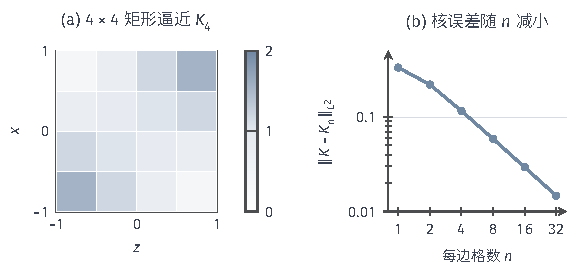
\includegraphics[width=97.4mm]{figures/02-abstract-mathematics/03-function-spaces/tikz/c3-rectangle-kernel/figure.pdf}
  \caption{用矩形示性函数的线性组合逼近核$K(x,z)=1+xz$（测度$dz/2$的乘积）。(a) $4\times4$均匀网格上取格内平均得到的分片常数核$K_4$，每格对应一个矩形$B_i\times A_j$。(b) $n\times n$网格平均的误差$\|K-K_n\|_{L^2}$，从$n=1$时的$1/3$降到$n=32$时约$0.015$，大致按$1/n$下降；它同时是相应有限秩算子的算子范数误差上界。}
  \label{fig:ose-rectangle-kernel}
\end{figure}

图~\ref{fig:ose-rectangle-kernel}在贯穿例子上演示第二步。用$n\times n$网格上的格内平均作分片常数核$K_n$，它是$n^2$个矩形示性函数的线性组合，对应的积分算子秩不超过$n$。格宽为$h=2/n$时，误差平方等于各格中$(xz-\bar x_i\bar z_j)^2$的平均，其中$\bar x_i,\bar z_j$为格中心；直接计算得$n=1,2,4,8$时误差约为$0.333$、$0.220$、$0.116$、$0.059$。对这个核，分片常数逼近远不是最经济的：$K$本身秩为$2$，截断奇异值分解两项就精确。矩形逼近的价值在于它对任意平方可积核都可行，从而在不知道奇异值的情况下证明了紧性。

\subsection{核的对称性与算子伴随}
\label{sec:ose-kernel-symmetry}

第~\ref{sec:ose-spectral-theorem}小节的谱分解要求算子自伴。本小节说明，对平方可积核，伴随算子仍是积分算子，其核由原核交换变量并取共轭得到；由此可以直接从核判断自伴性。

\paragraph{伴随核}
伴随由等式$\langle g,Tf\rangle=\langle T^*g,f\rangle$确定。左边是一个二重积分，只要能交换积分次序，就可以把对$y$的积分移到$g$一侧，读出$T^*g$的公式。

\begin{theorem}[伴随核]
\label{thm:ose-adjoint-kernel}
在定理~\ref{thm:ose-hs-bounded}的条件下，$T:L^2(\mu)\to L^2(\nu)$的伴随$T^*:L^2(\nu)\to L^2(\mu)$是以
\[
  K^*(x,y)=\overline{K(y,x)}
\]
为核的积分算子，即$(T^*g)(x)=\int_Y\overline{K(y,x)}g(y)\,d\nu(y)$。
\end{theorem}

\begin{proof}
任取$f\in L^2(\mu)$、$g\in L^2(\nu)$。函数$(y,x)\mapsto|g(y)||K(y,x)||f(x)|$在乘积空间上可积：由乘积空间中的Cauchy–Schwarz不等式，它的积分不超过$\|K\|_{L^2}$乘以$(y,x)\mapsto|g(y)f(x)|$的$L^2$范数，后者由Tonelli定理等于$\|g\|\|f\|$。于是可以用Fubini定理交换积分次序：
\[
  \begin{aligned}
  \langle g,Tf\rangle&=\int_Y\overline{g(y)}\int_XK(y,x)f(x)\,d\mu(x)\,d\nu(y)\\
  &=\int_X\overline{\Bigl(\int_Y\overline{K(y,x)}g(y)\,d\nu(y)\Bigr)}f(x)\,d\mu(x).
  \end{aligned}
\]
括号中的函数正是以$K^*$为核的积分算子作用于$g$，且$K^*\in L^2(\mu\otimes\nu)$，由定理~\ref{thm:ose-hs-bounded}它属于$L^2(\mu)$。上式说明它满足伴随的定义式$\langle g,Tf\rangle=\langle T^*g,f\rangle$；由伴随的唯一性，它就是$T^*g$。
\end{proof}

伴随核把原核的输入、输出两个变量互换，在实值情形下就是关于对角线作镜像。图~\ref{fig:ose-kernel-adjoint}以例~\ref{ex:ose-volterra-svd}中的积分算子为例：$K(x,t)=\mathbf 1_{\{t<x\}}$在对角线上方取一，表示$(Vf)(x)$累积$x$左边的输入；伴随核在对角线下方取一，表示$(V^*g)(t)=\int_t^1g$累积$t$右边的输入。这正是例中通过交换积分次序得到的公式。

\begin{figure}[!htb]
  \centering
  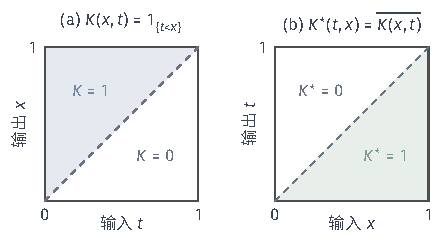
\includegraphics[width=75.2mm]{figures/02-abstract-mathematics/03-function-spaces/tikz/c3-kernel-adjoint/figure.pdf}
  \caption{积分核与伴随核关于对角线互为镜像。(a) $(Vf)(x)=\int_0^xf$的核$K(x,t)=\mathbf 1_{\{t<x\}}$，纵轴为输出变量，阴影处取值$1$。(b) 伴随核$K^*(t,x)=\overline{K(x,t)}=\mathbf 1_{\{x>t\}}$，给出$(V^*g)(t)=\int_t^1g$。两核不相等，所以$V$不自伴。}
  \label{fig:ose-kernel-adjoint}
\end{figure}

\paragraph{对称核与自伴}
当$X=Y$且$\mu=\nu$时，若$K(x,z)=\overline{K(z,x)}$对$\mu\otimes\mu$几乎处处的$(x,z)$成立，则$K^*=K$几乎处处，由定理~\ref{thm:ose-adjoint-kernel}得$T^*=T$，$T$是紧自伴算子。这时定理~\ref{thm:ose-compact-selfadjoint}的谱分解可以直接使用。实值核的这一条件就是对称性$K(x,z)=K(z,x)$。贯穿例子的$1+xz$是实对称核，所以它的特征函数$1$与$\sqrt3x$正交、特征值是实数，与第~\ref{sec:ose-spectral-theorem}小节的计算一致；积分算子$V$的核不对称，它的左右奇异函数是两组不同的三角函数。

\paragraph{对称不等于正}
自伴只说明二次型$\langle f,Tf\rangle$是实数，并不保证它非负。核$1-6xz$实对称，但取$f=x$得$Tf=-2x$，
\[
  \langle f,Tf\rangle=\int x\cdot(-2x)\,d\mu=-\tfrac23<0 .
\]
相比之下，$1+xz$给出$\langle f,Tf\rangle=|\int f\,d\mu|^2+|\int xf\,d\mu|^2\geq0$，是正算子。正性要单独检查，不能从核对称推出。

\paragraph{等价类与点值}
平方可积核本身只是$\nu\otimes\mu$几乎处处的等价类。在零测集上改动核不改变积分算子，却可能完全改变它在个别点上的取值。例如在$[-1,1]^2$上令$K'(x,z)=1+xz-10\cdot\mathbf 1_{\{x=z\}}$，对角线在乘积测度下为零测集，所以$K'$与$K$给出同一个正算子；但$K'(x,x)=x^2-9<0$，单点$\{x\}$上的$1\times1$“Gram矩阵”为负。因此，从本节的$L^2$结论出发，不能谈论“所有有限点集上的Gram矩阵是否半正定”，也不能谈论核在指定点上的再生关系。这些问题需要核取连续代表、并对所有有限点集半正定，属于第~\ref{sec:rkhs-point-evaluation}节及第~\ref{sec:rkhs-mercer}节的内容。

% 第3章第4节：积分方程的可解性与稳定性（两类方程、小范数迭代、紧算子的Fredholm二择、第一类方程与小奇异值）。

\section{积分方程的可解性与稳定性}
\label{sec:ose-integral-equations}

前三节都在正向使用算子：给定输入，计算输出。本节反过来，把积分算子放进未知函数满足的方程，依次回答章首的三个问题：解是否存在、是否唯一、对数据的误差是否稳定。两类方程的像空间结构截然不同，所以分开处理：第二类方程在小范数条件下可以直接迭代求解，在紧性条件下有完整的可解性判别；第一类方程还要面对小奇异值带来的放大。

\subsection{第一类与第二类积分方程}
\label{sec:ose-equation-types}

\paragraph{两类方程}
设$T$是积分算子，$g$是已知函数，$f$是未知函数。若$T:H_1\to H_2$，方程
\begin{equation}
  Tf=g
  \label{eq:ose-first-kind}
\end{equation}
称为\term{第一类积分方程}（integral equation of the first kind），此时$g$是观察到的输出，要求恢复产生它的输入。若$T:H\to H$，$\lambda\in\mathbb F$为参数，方程
\begin{equation}
  (I-\lambda T)f=g,\qquad\text{即}\quad f(x)-\lambda\int K(x,z)f(z)\,d\mu(z)=g(x),
  \label{eq:ose-second-kind}
\end{equation}
称为\term{第二类积分方程}（integral equation of the second kind），此时$g$是源项，未知函数同时出现在积分内外。两类方程的区别不在于写法：第二类方程中，未知函数在积分之外还有一个单位算子的“副本”，这个副本保证了在积分算子看不见的方向上，信息不会丢失。

\paragraph{贯穿例子中的两类方程}
回到$L^2([-1,1],\mu)$、$d\mu=dz/2$、$K(x,z)=1+xz$。由第~\ref{sec:ose-spectral-theorem}小节，任意$f$可以分解为$f=\alpha+\beta x+h$，其中$h$与$1,x$都正交，并且$Tf=\alpha+\frac{\beta}{3}x$。

第一类方程$Tf=g$只能产生一次函数，所以只有当$g=a+bx$时才有解。此时$\alpha=a$、$\beta=3b$，而$h$完全不受约束：
\[
  f=a+3bx+h,\qquad h\perp1,\ h\perp x .
\]
解存在时有无穷多个，差别正是$\ker T$中的任意元素，这个核是无限维的。

第二类方程$(I-\lambda T)f=g$则不同。把$g$同样分解为$g=a+bx+k$，$k$与$1,x$正交，逐方向比较系数得
\[
  (1-\lambda)\alpha=a,\qquad\Bigl(1-\frac{\lambda}{3}\Bigr)\beta=b,\qquad h=k .
\]
只要$\lambda\neq1,3$，每个$g$都给出唯一解；例如$\lambda=1/2$时$f=2a+\frac65bx+k$。图~\ref{fig:ose-equation-types}比较两类方程在各方向上的乘子：第一类方程把与$1,x$正交的方向全部乘以零，第二类方程在这些方向上保留单位作用，只在两个特征方向上改变比例。

\begin{figure}[!htb]
  \centering
  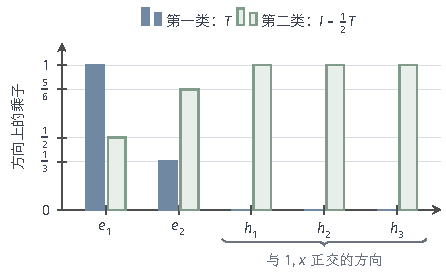
\includegraphics[width=75.5mm]{figures/02-abstract-mathematics/03-function-spaces/tikz/c3-equation-types/figure.pdf}
  \caption{核$1+xz$（测度$dz/2$）给出的两类方程在各正交方向上的乘子。$e_1=1$、$e_2=\sqrt3x$为特征方向，$h_1,h_2,h_3$代表与它们正交的方向（如$x^2-1/3$）。深色：第一类方程的算子$T$，在正交方向上为零，信息丢失；浅色：第二类方程的算子$I-\frac12T$，在正交方向上恒为$1$。}
  \label{fig:ose-equation-types}
\end{figure}

\paragraph{核、像与例外参数}
同一个例子已经显示出两类方程各自的困难。第一类方程的困难来自$T$本身：$\ker T$非零造成不唯一，$\operatorname{Ran}T$不是全空间造成不存在。第二类方程只在特殊参数处出问题：$\lambda=1$时齐次方程$(I-T)f=0$有非零解$f=1$，$\lambda=3$时有非零解$f=x$；这两个参数正是特征值$1$与$1/3$的倒数。

由此形成本节其余部分的分工。第~\ref{sec:ose-neumann}小节说明，当$\|\lambda T\|<1$时，第二类方程可以用级数和迭代直接构造解；第~\ref{sec:ose-fredholm}小节用紧性给出第二类方程对所有参数的可解性判别；第~\ref{sec:ose-first-kind}小节回到第一类方程，说明除了正交条件，还需要控制反演时被除掉的小奇异值。

\subsection{小范数条件下的解与迭代}
\label{sec:ose-neumann}

\paragraph{Neumann级数}
标量方程$(1-q)x=g$在$|q|<1$时有解$x=\sum_{n\geq0}q^ng$。算子方程可以照此办理，只要几何级数在算子范数下收敛。第~\ref{sec:lfo-operator-space}节已经证明，$X$为Banach空间时$\mathcal B(X)$在算子范数下完备，这正是让级数收敛所需要的。

\begin{theorem}[Neumann级数]
\label{thm:ose-neumann}
设$X$为Banach空间，$S\in\mathcal B(X)$且$\|S\|<1$。则$I-S$可逆，逆算子有界，并且
\[
  (I-S)^{-1}=\sum_{n=0}^{\infty}S^n,\qquad\|(I-S)^{-1}\|\leq\frac{1}{1-\|S\|},
\]
级数按算子范数收敛。
\end{theorem}

\begin{proof}
由$\|S^n\|\leq\|S\|^n$，级数$\sum_n\|S^n\|$被收敛的几何级数控制，部分和$P_N=\sum_{n=0}^{N}S^n$在$\mathcal B(X)$中是柯西列，由完备性收敛到某个$P$，且$\|P\|\leq\sum_n\|S\|^n=1/(1-\|S\|)$。部分和满足望远镜恒等式
\[
  P_N(I-S)=(I-S)P_N=I-S^{N+1},
\]
而$\|S^{N+1}\|\leq\|S\|^{N+1}\to0$。令$N\to\infty$，由算子乘法对算子范数连续，得$P(I-S)=(I-S)P=I$。
\end{proof}

由该级数定义的
\[
  \sum_{n=0}^{\infty}S^n
\]
称为\term{Neumann级数}（Neumann series）。取$S=\lambda T$，当$\|\lambda T\|<1$时，第二类方程~\eqref{eq:ose-second-kind}对每个$g$有唯一解$f=\sum_n\lambda^nT^ng$，且$\|f\|\leq\|g\|/(1-|\lambda|\|T\|)$。数据误差的影响由同一个界控制：若源项从$g$变为$\tilde g$，解的变化不超过$\|g-\tilde g\|/(1-\|\lambda T\|)$。

\paragraph{压缩迭代}
Neumann级数的部分和可以逐步计算。令$\Phi(f)=g+\lambda Tf$，则方程~\eqref{eq:ose-second-kind}等价于不动点方程$f=\Phi(f)$。从$f_0$出发迭代$f_{n+1}=\Phi(f_n)$，展开得
\[
  f_n=\sum_{k=0}^{n-1}(\lambda T)^kg+(\lambda T)^nf_0 ,
\]
即Neumann级数的部分和加上一项逐渐消失的初值影响。这个迭代满足本卷“度量空间”章压缩映射定理（定理~\ref{thm:metric-contraction}）的全部条件：$X$完备；$\Phi$把$X$映入自身；对任意$f,h$有
\[
  \|\Phi(f)-\Phi(h)\|=\|\lambda T(f-h)\|\leq q\|f-h\|,\qquad q=\|\lambda T\|<1 .
\]
压缩常数$q$对所有输入统一成立，这是压缩映射定理要求的，也是小范数条件提供的。

\paragraph{误差估计}
压缩映射定理的先验估计~\eqref{eq:metric-a-priori}直接给出
\[
  \|f_n-f_*\|\leq\frac{q^n}{1-q}\|f_1-f_0\| .
\]
若每步迭代都带有执行误差，即实际计算的$f_{n+1}$满足$\|f_{n+1}-\Phi(f_n)\|\leq\eta_n$，记$e_n=\|f_n-f_*\|$，第~\ref{sec:metric-inexact-contraction}节的递推~\eqref{eq:metric-inexact-error}给出$e_{n+1}\leq qe_n+\eta_n$。在$\eta_n\leq\eta$时，展开递推得到$\limsup_ne_n\leq\eta/(1-q)$：每步的执行误差被放大$1/(1-q)$倍，形成一个误差地板。$q$接近$1$时，即使每步误差很小，最终误差也可能很大。

\begin{example}[迭代求解第二类方程]
\label{ex:ose-neumann-iteration}
在贯穿例子中取$\lambda=1/2$，$g=1+x$。此时$q=\|\frac12T\|=\frac12$。由前一小节的系数关系，精确解为$f_*=2+\frac65x$。从$f_0=0$迭代，常数系数满足$a_{n+1}=1+\frac12a_n$，$x$的系数满足$b_{n+1}=1+\frac16b_n$，所以
\[
  a_n=2\bigl(1-2^{-n}\bigr),\qquad b_n=\tfrac65\bigl(1-6^{-n}\bigr),
\]
误差为
\[
  \|f_n-f_*\|^2=\bigl(2\cdot2^{-n}\bigr)^2+\tfrac13\bigl(\tfrac65\cdot6^{-n}\bigr)^2 .
\]
这里用到$\|\alpha+\beta x\|^2=|\alpha|^2+|\beta|^2/3$。先验界为$\frac{2^{-n}}{1/2}\|g\|=2\cdot2^{-n}\cdot\frac{2}{\sqrt3}$，比实际误差略大。若每步都多加一个$-10^{-3}$的常数偏差，常数系数改为收敛到$2-2\times10^{-3}$，误差停在$2\times10^{-3}=\eta/(1-q)$，恰好达到误差地板。
\end{example}

\begin{figure}[!htb]
  \centering
  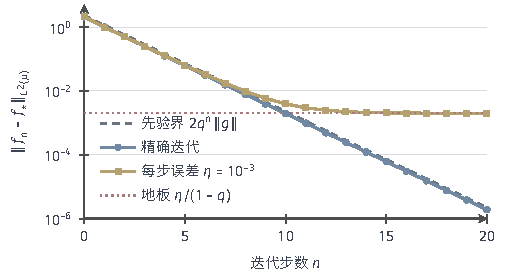
\includegraphics[width=85.7mm]{figures/02-abstract-mathematics/03-function-spaces/tikz/c3-neumann-error/figure.pdf}
  \caption{第二类方程$(I-\frac12T)f=1+x$（核$1+xz$，测度$dz/2$）的不动点迭代误差，纵轴取对数。虚线：先验界$q^n\|f_1-f_0\|/(1-q)$，$q=1/2$；圆点：精确迭代，误差几乎按$2^{-n}$下降；方点：每步带有大小$\eta=10^{-3}$的常数偏差，误差停在点线所示的地板$\eta/(1-q)=2\times10^{-3}$。}
  \label{fig:ose-neumann-error}
\end{figure}

图~\ref{fig:ose-neumann-error}画出例~\ref{ex:ose-neumann-iteration}的三条曲线。精确迭代的误差几乎贴着先验界下降，速度由最慢的方向$a_n$的比例$1/2$决定；带执行误差的迭代起初与精确迭代重合，大约十步后停在地板上，继续迭代不再改进。

\paragraph{小范数只是充分条件}
$\|\lambda T\|<1$保证可解，但不是可解的必要条件。最简单的例子是$B=2I$：$\|B\|=2$，Neumann级数$\sum_nB^n=\sum_n2^nI$发散，迭代$f_{n+1}=g+2f_n$从$f_0=0$出发给出$f_n=(2^n-1)g$，也发散；可是$I-B=-I$显然可逆，方程$(I-B)f=g$的唯一解为$f=-g$。这里的$B$不是用平方可积核表示的积分算子，只用来说明一般算子的情形。

积分方程中也有同样的现象。贯穿例子中取$\lambda=2$，则$\|\lambda T\|=2$，但$\lambda\neq1,3$，方程$(I-2T)f=g$对每个$g=a+bx+k$有唯一解$f=-a+3bx+k$。迭代的常数系数却满足$a_{n+1}=a+2a_n$，只要$a\neq0$就发散。方程可解与某个迭代法收敛是两件事；要判断前者，需要下一小节的工具。

\subsection{紧算子条件下的可解性}
\label{sec:ose-fredholm}

小范数条件把第二类方程限制在$|\lambda|<1/\|T\|$的范围内。对紧算子，我们能对所有参数给出完整的判别。先在紧自伴情形中用特征方向看清答案，再对一般紧算子给出证明。

\paragraph{紧自伴情形的方向解释}
设$T$为紧自伴算子，按定理~\ref{thm:ose-compact-selfadjoint}有特征对$(\lambda_j,e_j)$及$u=u_0+\sum_jc_je_j$，其中$u_0\in\ker T$，$c_j=\langle e_j,u\rangle$。则
\[
  (I-\lambda T)u=u_0+\sum_j(1-\lambda\lambda_j)c_je_j .
\]
$I-\lambda T$在核方向上作用为$1$，在第$j$个特征方向上乘以$1-\lambda\lambda_j$。若$\lambda$不等于任何$1/\lambda_j$，这些乘子都非零；又因为$\lambda_j\to0$，乘子趋于$1$，所以$\inf_j|1-\lambda\lambda_j|>0$。逐方向除以乘子就得到有界逆：
\[
  f=g_0+\sum_j\frac{\langle e_j,g\rangle}{1-\lambda\lambda_j}e_j ,\qquad g_0\text{为}g\text{在}\ker T\text{上的分量}.
\]
若$\lambda=1/\lambda_k$，乘子在$\lambda_k$的特征空间上为零，这个有限维特征空间就是齐次方程的解空间$\ker(I-\lambda T)$；方程可解当且仅当$g$在这些方向上的系数为零，即$g\perp\ker(I-\lambda T)$，此时解可以加上该特征空间中的任意元素。$\lambda$为实数，$I-\lambda T$自伴，所以这里的正交条件也就是$g\perp\ker(I-\lambda T)^*$。

图~\ref{fig:ose-fredholm-alternative}在贯穿例子上画出三个乘子随$\lambda$的变化。常数方向的乘子$1-\lambda$在$\lambda=1$处为零，线性方向的乘子$1-\lambda/3$在$\lambda=3$处为零，正交补方向的乘子恒为$1$。除这两个例外参数外，方程总是唯一可解的；$\lambda=1/2$与$\lambda=2$都在这个范围内，尽管只有前者满足小范数条件。

\begin{figure}[!htb]
  \centering
  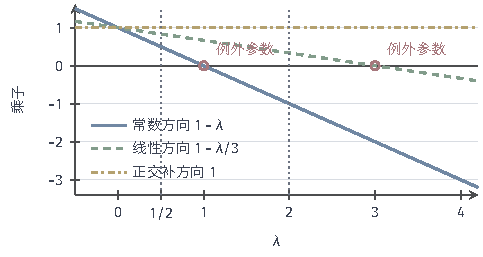
\includegraphics[width=81.8mm]{figures/02-abstract-mathematics/03-function-spaces/tikz/c3-fredholm-alternative/figure.pdf}
  \caption{第二类方程$(I-\lambda T)f=g$在各方向上的乘子随参数$\lambda$的变化（核$1+xz$，测度$dz/2$）。乘子为零的$\lambda=1$与$\lambda=3$（空心圆）是例外参数，齐次方程在此有非零解；其余参数下方程唯一可解。点线标出$\lambda=1/2$（满足小范数条件）与$\lambda=2$（不满足，但仍唯一可解）。}
  \label{fig:ose-fredholm-alternative}
\end{figure}

\paragraph{Fredholm二择定理}
对一般紧算子，没有正交特征基可用，但结论的形式保持不变。

\begin{theorem}[Fredholm二择定理]
\label{thm:ose-fredholm}
设$H$为Hilbert空间，$T:H\to H$为紧算子，$\lambda\in\mathbb F$，$B=I-\lambda T$。则：
\begin{enumerate}
  \item $\ker B$与$\ker B^*$都是有限维的；
  \item $\operatorname{Ran}B$是闭子空间，因而$\operatorname{Ran}B=(\ker B^*)^\perp$；
  \item $\ker B=\{0\}$当且仅当$\operatorname{Ran}B=H$，此时$B^{-1}$有界。
\end{enumerate}
因此以下二者恰有一个成立：齐次方程$Bf=0$只有零解，此时对每个$g\in H$，方程$Bf=g$有唯一解，且解有界地依赖于$g$；或者齐次方程有非零解，此时$Bf=g$可解当且仅当$g\perp\ker B^*$，全部解为一个特解加上$\ker B$中的任意元素。
\end{theorem}

这个结论称为\term{Fredholm二择定理}（Fredholm alternative）。它的力量在于第二条：像空间闭合是事先由紧性保证的，所以正交条件$g\perp\ker B^*$判断的是\emph{精确}可解，而不只是$g$能否被输出逼近。对比第~\ref{sec:lfo-range-kernel}节中的$A(x_n)=(x_n/n)$：$\ker A^*=\{0\}$，每个$y$都满足正交条件，但$(1/n)$并不在像中，因为$\operatorname{Ran}A$不闭。还可以证明$\dim\ker B=\dim\ker B^*$，这里不需要这一结论，不再展开。

\paragraph{证明思路：有限秩加小范数余项}
证明把紧算子拆成两部分：有限秩部分化为有限维线性方程组，余项部分用Neumann级数吸收。$\lambda=0$时$B=I$，结论显然，下面设$\lambda\neq0$。

\begin{proof}
第一步，分解。由定理~\ref{thm:ose-finite-rank-approx}，取有限秩算子$F$使$\|\lambda(T-F)\|<1$。记$C=I-\lambda(T-F)$，由定理~\ref{thm:ose-neumann}，$C$可逆且$C,C^{-1}$都有界。于是
\[
  B=C-\lambda F=C(I-G),\qquad G=\lambda C^{-1}F .
\]
$G$仍是有限秩算子。取$\operatorname{Ran}G$的一组线性无关基$b_1,\ldots,b_r$，则$Gf=\sum_{i=1}^r\ell_i(f)b_i$，系数$\ell_i$是有界线性泛函，由Riesz表示（第~\ref{sec:lfo-riesz}节）写成$\ell_i(f)=\langle a_i,f\rangle$。

第二步，化为矩阵方程。令$\bm M_{i,j}=\langle a_i,b_j\rangle$，$\bm d(h)=(\langle a_1,h\rangle,\ldots,\langle a_r,h\rangle)^\top$。我们断言：$(I-G)f=h$当且仅当$f=h+\sum_ic_ib_i$，其中$\bm c=(c_1,\ldots,c_r)^\top$满足$(\bm I-\bm M)\bm c=\bm d(h)$。若$(I-G)f=h$，则$f=h+Gf=h+\sum_ic_ib_i$，其中$c_i=\langle a_i,f\rangle=\langle a_i,h\rangle+\sum_j\bm M_{i,j}c_j$。反过来，若$\bm c$满足矩阵方程，令$f=h+\sum_jc_jb_j$，则$Gf=\sum_i\bigl(\bm d(h)_i+(\bm M\bm c)_i\bigr)b_i=\sum_ic_ib_i=f-h$。

第三步，核有限维、像闭合。取$h=0$，$\ker(I-G)$由$\ker(\bm I-\bm M)$经单射$\bm c\mapsto\sum_ic_ib_i$得到，维数不超过$r$；$C$可逆，所以$\ker B=\ker(I-G)$有限维。由第二步，$h\in\operatorname{Ran}(I-G)$当且仅当$\bm d(h)\in\operatorname{Ran}(\bm I-\bm M)$。$\mathbb F^r$的子空间$\operatorname{Ran}(\bm I-\bm M)$是有限个线性泛函的公共零点，与连续映射$\bm d$复合后，$\operatorname{Ran}(I-G)$是$H$上有限个连续线性泛函的公共零点，因而闭。$C$与$C^{-1}$都连续，所以$\operatorname{Ran}B=C\bigl(\operatorname{Ran}(I-G)\bigr)$也闭。

第四步，单射推出满射。若$\ker B=\{0\}$，则$\ker(\bm I-\bm M)=\{0\}$，有限维方阵$\bm I-\bm M$可逆，矩阵方程对每个$\bm d(h)$有解，于是$I-G$满射，$B=C(I-G)$也满射。反之，若$B$满射，则$\ker B^*=(\operatorname{Ran}B)^\perp=\{0\}$；对下一步说明的紧算子$T^*$应用本步，$B^*$满射，从而$\ker B=(\operatorname{Ran}B^*)^\perp=\{0\}$。双射$B$的逆有界由第~\ref{sec:lfo-open-mapping}节的有界逆定理保证。

第五步，处理伴随。若$F_n$是有限秩算子且$\|T-F_n\|\to0$，则$F_n^*$也是有限秩的（$F_nf=\sum_i\langle a_i,f\rangle b_i$时$F_n^*g=\sum_i\langle b_i,g\rangle a_i$），且$\|T^*-F_n^*\|=\|T-F_n\|\to0$，由定理~\ref{thm:ose-compact-limit}，$T^*$是紧算子。$B^*=I-\overline\lambda T^*$与$B$同型，由第三步，$\ker B^*$有限维。最后，像闭合且由第~\ref{sec:lfo-range-kernel}节$\overline{\operatorname{Ran}B}=(\ker B^*)^\perp$，得$\operatorname{Ran}B=(\ker B^*)^\perp$。
\end{proof}

第三步中，有限维的矩阵方程决定了无限维方程的全部可解性：无限维部分已经被可逆的$C$吸收。这也说明了紧性的作用：若$T$不能被有限秩算子逼近，就无法把问题化到有限维。

\paragraph{两个推论}
定理的第三条有一个直接推论：紧算子$T$的非零谱点都是特征值。若$\mu\neq0$不是特征值，取$\lambda=1/\mu$，则$I-\lambda T$是单射，由定理是有界可逆的，于是$T-\mu I=-\mu(I-\lambda T)$也有界可逆，$\mu\in\rho(T)$。结合第~\ref{sec:ose-spectrum-def}小节，无限维空间中紧算子的谱由至多可数个非零特征值和$0$组成。

另一个推论关于迭代。Fredholm二择告诉我们方程何时可解，但没有给出求解的迭代格式。第~\ref{sec:ose-neumann}小节中$\lambda=2$的例子正处于“唯一可解但迭代发散”的情形：定理~\ref{thm:ose-fredholm}保证解存在、有界依赖于数据，固定点迭代仍受$\|\lambda T\|<1$的收缩条件限制。

\subsection{第一类方程与小奇异值}
\label{sec:ose-first-kind}

第一类方程$Tf=g$没有单位算子的“副本”，紧算子$T$的像一般不闭，Fredholm二择的结论不再适用。本小节用奇异值分解给出精确可解的条件，并说明为什么即使解存在，它也可能对数据极其敏感。

\paragraph{精确可解的Picard条件}
设$T:H_1\to H_2$为紧算子，奇异值分解为$Tx=\sum_j\sigma_j\langle v_j,x\rangle u_j$。若$Tf=g$，则对每个$j$，
\[
  \langle u_j,g\rangle=\langle u_j,Tf\rangle=\langle T^*u_j,f\rangle=\sigma_j\langle v_j,f\rangle ,
\]
所以$f$在$v_j$方向上的系数只能是$\langle u_j,g\rangle/\sigma_j$。这些系数必须平方可和，$f$才属于$H_1$。

\begin{theorem}[第一类方程的可解性与最小范数解]
\label{thm:ose-picard}
设$T:H_1\to H_2$为紧算子，奇异值分解如定理~\ref{thm:ose-svd}。则$Tf=g$有解，当且仅当以下两条同时成立：
\begin{equation}
  g\perp\ker T^*,\qquad \sum_j\frac{|\langle u_j,g\rangle|^2}{\sigma_j^2}<\infty .
  \label{eq:ose-picard}
\end{equation}
此时
\[
  f^\dagger=\sum_j\frac{\langle u_j,g\rangle}{\sigma_j}v_j
\]
是唯一属于$(\ker T)^\perp$的解，全部解为$f^\dagger+\ker T$，且$f^\dagger$是范数最小的解。
\end{theorem}

\begin{proof}
必要性：若$Tf=g$，则$g\in\operatorname{Ran}T\subseteq(\ker T^*)^\perp$；由上面的系数关系和Bessel不等式，$\sum_j|\langle u_j,g\rangle|^2/\sigma_j^2=\sum_j|\langle v_j,f\rangle|^2\leq\|f\|^2$。

充分性：第二个条件使级数$f^\dagger$按范数收敛（第~\ref{sec:fs-orthogonal-expansion}节），且$f^\dagger$属于$(v_j)$的闭张成$(\ker T)^\perp$。由连续性逐项作用，$Tf^\dagger=\sum_j\langle u_j,g\rangle u_j$，这是$g$在$(u_j)$的闭张成上的正交投影。由定理~\ref{thm:ose-svd}，这个闭张成等于$(\ker T^*)^\perp$，而第一个条件说明$g$就在其中，所以$Tf^\dagger=g$。

解的结构：两个解之差属于$\ker T$，故全部解为$f^\dagger+\ker T$。$(\ker T)^\perp$中的解唯一，因为两个这样的解之差同时属于$\ker T$与$(\ker T)^\perp$。对任意解$f=f^\dagger+h$，$h\in\ker T$与$f^\dagger$正交，由勾股定理$\|f\|^2=\|f^\dagger\|^2+\|h\|^2\geq\|f^\dagger\|^2$。
\end{proof}

式~\eqref{eq:ose-picard}中的第二个条件称为\term{Picard条件}（Picard condition），$f^\dagger$称为\term{最小范数解}（minimum-norm solution）。两个条件分工不同：第一个只保证$g$位于像的闭包中，即$g$能被输出任意逼近；第二个才保证形式逆像$\sum_j\sigma_j^{-1}\langle u_j,g\rangle v_j$真正属于输入空间。

\paragraph{Picard条件的例子}
在贯穿例子中，$T$只有两个奇异值$1$与$1/3$，Picard条件自动成立，第一个条件就是$g\in\operatorname{span}\{1,x\}$；对$g=a+bx$，最小范数解为$f^\dagger=a+3bx$，与第~\ref{sec:ose-equation-types}小节的结果一致，它正是全部解中去掉核分量$h$的那一个。

$\ell^2$上的$A(x_n)=(x_n/n)$说明两个条件确实不同。$A$自伴且单射，$\ker A^*=\{0\}$，第一个条件对所有$g$成立；奇异值$\sigma_n=1/n$，Picard条件化为$\sum_nn^2|g_n|^2<\infty$。图~\ref{fig:ose-picard-coefficients}比较两组数据：$g^{(1)}_n=1/n^2$的形式解系数为$1/n$，平方可和，$g^{(1)}=A(1/n)$；$g^{(2)}_n=1/n$本身平方可和，但形式解系数恒为$1$，不平方可和，所以$g^{(2)}$不在像中。这正是第~\ref{sec:lfo-range-kernel}节的例子，现在由Picard条件统一解释。

\begin{figure}[!htb]
  \centering
  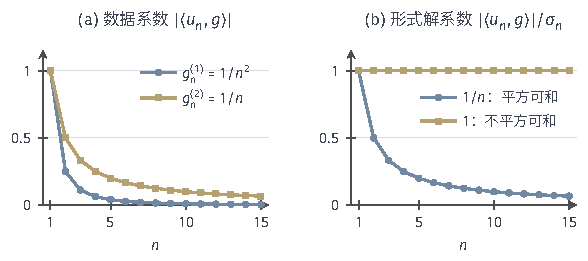
\includegraphics[width=99.6mm]{figures/02-abstract-mathematics/03-function-spaces/tikz/c3-picard-coefficients/figure.pdf}
  \caption{$\ell^2$上$A(x_n)=(x_n/n)$的Picard条件。(a) 两组数据的系数$1/n^2$与$1/n$，都平方可和，都满足$g\perp\ker A^*$。(b) 除以奇异值$\sigma_n=1/n$后的形式解系数：前者为$1/n$，平方可和，方程可解；后者恒为$1$，不平方可和，方程无解。}
  \label{fig:ose-picard-coefficients}
\end{figure}

对例~\ref{ex:ose-volterra-svd}的积分算子$V$，若$g$绝对连续、$g(0)=0$且$g'\in L^2(0,1)$，分部积分并利用$\cos\omega_k=0$可得$\langle u_k,g\rangle=\sigma_k\langle v_k,g'\rangle$，于是Picard级数等于$\sum_k|\langle v_k,g'\rangle|^2=\|g'\|^2$，最小范数解就是$f^\dagger=g'$。求解第一类方程$Vf=g$就是求导，这与微分运算的不稳定性一致。

\paragraph{小奇异值放大扰动}
即使解存在，它对数据的依赖也可能没有统一的界。设$T$有无限多个正奇异值，$\sigma_j\to0$。取数据扰动$\delta g_j=\sigma_ju_j$，则$\|\delta g_j\|=\sigma_j\to0$；它满足Picard条件，相应的最小范数解扰动为
\[
  \delta f_j=\frac{\langle u_j,\delta g_j\rangle}{\sigma_j}v_j=v_j,\qquad\|\delta f_j\|=1 .
\]
数据误差趋于零，解的误差却始终为$1$。所以映射$g\mapsto f^\dagger$在$\operatorname{Ran}T$上无界；这也说明$\operatorname{Ran}T$不闭，否则$T$限制在$(\ker T)^\perp$上是到闭像的有界双射，由有界逆定理其逆有界。只有有限多个正奇异值时情况相反：$\|f^\dagger\|\leq\|g\|/\sigma_{\min}$，在贯穿例子中放大倍数至多为$3$。

\begin{figure}[!htb]
  \centering
  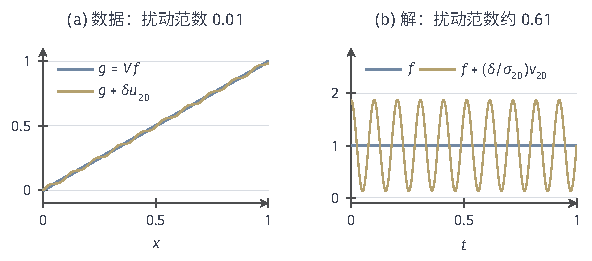
\includegraphics[width=100.2mm]{figures/02-abstract-mathematics/03-function-spaces/tikz/c3-noise-amplification/figure.pdf}
  \caption{第一类方程$Vf=g$（$(Vf)(x)=\int_0^xf$）中小奇异值放大扰动。真解$f=1$，数据$g=x$。(a) 数据加上范数为$0.01$的扰动$\delta u_{20}$，与原数据几乎重合。(b) 相应的最小范数解多出$(\delta/\sigma_{20})v_{20}$，振幅约$0.87$、范数约$0.61$，放大倍数$1/\sigma_{20}=19.5\pi\approx61$。}
  \label{fig:ose-noise-amplification}
\end{figure}

图~\ref{fig:ose-noise-amplification}在积分算子$V$上展示这一机制。数据中加入$\delta u_{20}$，$\delta=0.01$，曲线上几乎看不出差别；解中却多出振幅接近$0.87$的快速振荡。原因正是图~\ref{fig:ose-svd-decay}中看到的：$V$把快速振荡的输入平均掉，反解时必须把同样的振荡放大回去，振荡越快，放大倍数$1/\sigma_k=(k-\frac12)\pi$越大。

因此，第一类方程的解是否稳定，取决于数据在小奇异值方向上的成分。实际数据总带有误差，误差在所有方向上都有成分，直接计算$f^\dagger$会把高阶方向上的误差放大到失去意义。处理办法是舍去或压低小奇异值方向，例如只保留前$m$个奇异方向，或在求解目标中加入惩罚项；这些方法如何选择截断位置或惩罚强度、怎样平衡偏差与误差放大，属于优化问题，可参考\BookChapterRef{chap:optimization}{卷三“优化问题的定义与基本性质”章}及其后各章。从带噪观测中重建信号的具体任务，可参考\BookChapterRef{chap:signal-analysis}{卷三“信号”章}。

% 第3章第5节：本章小结。

\section{本章小结}
\label{sec:ose-summary}

章首的积分变换$Tf=\int(1+xz)f\,d\mu$只记住输入的两个矩，$\ell^2$上的$A(x_n)=(x_n/n)$则不丢掉任何方向，只是越往后压得越狠。本章围绕这两个例子，从三个角度描述一个变换：它能否用有限个方向统一逼近，各个方向被保留或压缩多少，以及从输出能否稳定地恢复输入。

紧性回答第一个问题。紧算子把有界输入族压成可以抽出收敛子列的输出族，并把弱收敛的输入变成范数收敛的输出。紧算子的算子范数极限仍是紧算子；在Hilbert空间中，紧算子恰好是有限秩算子的算子范数极限。这里的关键是“统一”：每个函数都能被截断逼近，并不意味着同一个有限维空间能以给定精度覆盖整个单位球的像，单位算子就是反例。

谱与奇异值回答第二个问题。无限维中谱不只由特征值组成，$A$的谱点$0$不对应任何被消去的方向，而对应一列越来越扁的方向和不闭的像。紧自伴算子有至多可数个实的非零特征值，只能在零处聚集，特征方向与核一起张满整个空间；一般紧算子用输入、输出两组方向写成奇异值分解，截断前$m$项的误差恰为$\sigma_{m+1}$，且是所有秩不超过$m$的逼近中最小的。这些展开都按Hilbert空间的范数成立，不自动给出逐点收敛。

积分核把上述结论具体化。核与测度一起确定算子；平方可积核给出有界的紧算子，证明的桥梁是用矩形示性函数的有限和逼近核；交换变量并取共轭得到伴随核，对称核给出自伴算子。但对称不保证正性，平方可积核作为等价类也谈不上点值和有限点集上的Gram矩阵。

第三个问题在两类方程上有不同的答案。第二类方程$(I-\lambda T)f=g$保留了单位算子，小范数时Neumann级数和压缩迭代直接给出解与误差界；对紧算子，Fredholm二择保证像闭合，于是要么唯一可解且稳定，要么在正交相容条件下可解、解差一个有限维核。第一类方程$Tf=g$还要满足Picard条件，而小奇异值使最小范数解对数据误差无界地敏感。几种判断不能互相替代：正交条件只在像闭合时判断精确可解，可解不等于某个迭代收敛，有解也不等于稳定。

这些认识是后续几类问题的起点。第~\ref{chap:rkhs}章给积分核加上连续性与半正定性，研究点值读取连续的函数空间，并在那里建立Mercer展开的逐点与一致收敛；带噪数据下怎样舍去或压低小奇异值方向，是优化中正则化的问题，具体的微分方程演化与信号重建则分别属于卷三的动力系统与信号部分。本章只保留算子方向与积分方程的共同基础，不预先引入这些任务各自的目标和算法。


\chapter{弱导数与Sobolev空间}
\label{chap:weak-derivatives-sobolev}

绝对值函数$|x|$在原点有一个尖点，经典导数在那里不存在；可是它两侧的斜率清清楚楚，分别是$-1$和$1$。阶跃函数在原点跳了一下，除原点外处处可导且导数为零，可没有人会说它“没有变化”。还有一类函数只按几乎处处等价类给出，例如第~\ref{chap:function-spaces}章里$L^p$空间的元素，谈论它在某一点的导数本身就没有意义。本章要回答的问题是：经典导数失效以后，怎样仍然保存“变化”的信息；当同时控制函数和它的变化时，又能对函数得到哪些结论。

关键的想法来自分部积分。对光滑函数$f$和在边界附近恒为零的光滑函数$\varphi$，有$\int f'\varphi=-\int f\varphi'$。右端不再要求$f$可导，只要求它能与$\varphi'$相乘再积分。于是可以反过来，用右端去\emph{定义}左端，把导数“转移”到光滑的测试函数上。第~\ref{sec:sob-distributions}节先确定哪些光滑函数可以充当测试，再把“对每个测试给出一个连续的线性读数”的对象称为广义函数；这一定义用到第~\ref{chap:linear-functionals-operators}章的线性泛函观点。广义函数总可以求导，但导数未必还是普通函数，$\delta_0$的导数就是一个例子。

第~\ref{sec:sob-weak-derivatives}节固定局部可积函数，问它的广义导数何时仍能由局部可积函数表示，并用尖点、跳跃和Cantor函数三个例子划出这一条件的边界；在一维情形，这个条件恰好等价于绝对连续。第~\ref{sec:sob-spaces}节把函数及其各阶弱导数的$L^p$大小同时放进范数，得到Sobolev空间，并证明它完备。第~\ref{sec:sob-smoothing}节说明怎样用光滑函数逼近Sobolev函数，这是后面许多证明先对光滑函数计算、再取极限的依据。第~\ref{sec:sob-regularity}节在这些工具上分别研究四个问题：导数的积分控制能否保证连续代表，有界函数列能否抽出强收敛子列，边界值怎样定义，以及去除常数方向后能否只用导数控制函数。

全章固定欧氏空间中的非空开集$\Omega\subset\mathbb R^d$与Lebesgue测度，函数可以取实值或复值。具体微分方程的弱解与演化、泛函的变分与最优条件、流形上的函数空间都不在这里展开；本章提供的是描述“导数受控的函数”所需的空间、微分运算和边界工具。

% 第4章第1节：测试函数与广义函数（紧支撑测试、局部配对、广义函数的定义与例子、广义函数的微分）。

\section{测试函数与广义函数}
\label{sec:sob-distributions}

要把导数转移到另一个函数上，先得有一批足够好的“另一个函数”：它们要光滑，才能承受任意次求导；要在区域边界附近恒为零，才能让分部积分不留下边界项。本节先构造这样的测试函数，并说明一列测试“变得很小”应当怎样理解；然后把对测试的连续线性读数称为广义函数，看它怎样同时容纳局部可积函数、点读数和测度；最后定义广义函数的导数，并用$\delta_0$的导数说明这一新对象确实超出了函数和测度的范围。

这里要先说明一个名称。本节的对象在文献中传统上称为“分布”（distribution），与概率论中的概率分布毫无关系。为避免混淆，本书称它为广义函数，只在必要时提到“分布”这个旧称。

\subsection{测试函数与局部配对}
\label{sec:sob-test-functions}

\paragraph{光滑凸起}
我们先在实轴上造一个光滑、却在一个区间外恒为零的函数。关键的一块是$s\mapsto e^{-1/s}$（$s>0$），并在$s\le0$处补成零。它在$s>0$的各阶导数都形如$p_k(1/s)\,e^{-1/s}$，其中$p_k$是多项式，这可以对求导次数归纳验证；由于对任意$m$都有$s^{-m}e^{-1/s}\to0$（$s\to0^+$），每一阶导数从右侧趋于零，与左侧的零相接。于是这个函数在整条实轴上无穷次可微，却在$s\le0$上恒为零。代入$s=1-t^2$，得到
\begin{equation}
 \psi(t)=
 \begin{cases}
  \exp\!\left(-\dfrac{1}{1-t^2}\right), & |t|<1,\\[1ex]
  0, & |t|\ge1,
 \end{cases}
 \label{eq:sob-bump}
\end{equation}
它无穷次可微，在$(-1,1)$内为正，在$[-1,1]$外为零，最大值$\psi(0)=e^{-1}$。图~\ref{fig:sob-bump-cutoff}(a)画出了这个凸起。

\begin{figure}[!htb]
  \centering
  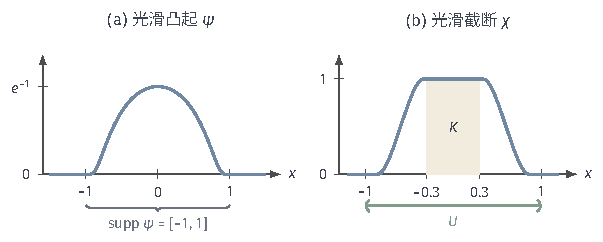
\includegraphics[width=102.2mm]{figures/02-abstract-mathematics/03-function-spaces/tikz/c4-bump-cutoff/figure.pdf}
  \caption{测试函数的两个基本构件。(a)~光滑凸起$\psi$，在$(-1,1)$内为正，在区间外恒为零，各阶导数在$\pm1$处都连续地接到零。(b)~光滑截断$\chi=\mathbf 1_{[-0.6,0.6]}*\rho_{0.3}$：在紧集$K=[-0.3,0.3]$（阴影）上恒为$1$，支撑$[-0.9,0.9]$落在开集$U=(-1,1)$内，中间光滑地由$1$降到$0$。}
  \label{fig:sob-bump-cutoff}
\end{figure}

在$\mathbb R^d$中，把$t^2$换成$|x|^2$就得到在单位开球内为正、在球外为零的光滑凸起$\psi(|x|)$，这里$|x|$是欧氏长度。平移伸缩为$\psi(|x-x_0|/r)$后，它的“非零区域”是以$x_0$为中心、半径为$r$的球。只要$r$小于$x_0$到$\Omega$边界的距离，这个凸起就整个待在$\Omega$内部，离边界还有一段间隔。

\paragraph{支撑与测试函数}
为了把“在边界附近恒为零”说准确，对函数$\varphi$定义它的\term{支撑}（support）
\[
 \operatorname{supp}\varphi=\overline{\{x:\varphi(x)\neq0\}},
\]
即非零点集合的闭包。记$C_c^\infty(\Omega)$为$\Omega$上无穷次可微、且支撑是$\Omega$的紧子集的函数全体，称其中的函数为\term{测试函数}（test function）。支撑紧含于$\Omega$，意味着它与边界保持正距离：存在$\delta>0$，使离边界不到$\delta$的点上$\varphi$恒为零。上面的平移凸起就是测试函数。

这一点立刻解决了分部积分的边界项。设$f\in C^1(\Omega)$，$\varphi\in C_c^\infty(\Omega)$。把$f\varphi$在$\Omega$外补成零，得到$\mathbb R^d$上紧支撑的$C^1$函数。沿第$j$个坐标方向的任一直线积分$\partial_j(f\varphi)$，由微积分基本定理得零，因为两端都落在支撑之外；再对其余坐标积分（Fubini定理~\ref{thm:analysis-fubini-integrable}），得到
\begin{equation}
 \int_\Omega(\partial_jf)\,\varphi\,\mathrm dx=-\int_\Omega f\,\partial_j\varphi\,\mathrm dx .
 \label{eq:sob-integration-by-parts}
\end{equation}
式~\eqref{eq:sob-integration-by-parts}没有边界项，并且右端已不再出现$f$的导数。本章后面的全部构造都从这个等式出发。

\paragraph{局部可积函数}
要让$\int_\Omega f\varphi\,\mathrm dx$有意义，$f$需要满足什么条件？测试函数只在一个紧集上非零，并且在那里有界，所以只需要$f$在每个紧集上可积。称可测函数$f$\term{局部可积}（locally integrable），若对每个紧集$K\subset\Omega$都有$\int_K|f|\,\mathrm dx<\infty$，记作$f\in L^1_{\mathrm{loc}}(\Omega)$；与$L^p$空间一样，几乎处处相等的函数视为同一元素。对$f\in L^1_{\mathrm{loc}}(\Omega)$和支撑在紧集$K$内的测试$\varphi$，
\begin{equation}
 \left|\int_\Omega f\varphi\,\mathrm dx\right|\le\left(\int_K|f|\,\mathrm dx\right)\sup_K|\varphi| ,
 \label{eq:sob-local-pairing}
\end{equation}
右端有限，配对良好定义，而且改变$f$在一个零测集上的值不影响积分。

局部可积比可积宽得多，也依赖于区域。$f(x)=1/x$在$(0,1)$上局部可积：$(0,1)$的紧子集离$0$有正距离，$1/x$在其上有界；但$\int_0^1 x^{-1}\,\mathrm dx=\infty$，所以它不在$L^1(0,1)$中。把区域换成整条实轴，任何含原点的紧区间上积分都发散，$1/x$便不再局部可积。再看$\mathbb R^d$中的幂函数$|x|^{-a}$：按例~\ref{ex:region-power-function-threshold}的二进壳层估计，$d$维壳层$\{2^k\le|x|<2^{k+1}\}$的体积按$2^{kd}$缩放，于是单位球上$\int|x|^{-a}\,\mathrm dx<\infty$当且仅当$a<d$。因此$|x|^{-a}\in L^1_{\mathrm{loc}}(\mathbb R^d)$当且仅当$a<d$。这个阈值在后面检验弱导数和嵌入时会反复使用。

\paragraph{光滑截断}
后面经常需要这样一个测试：它在一个给定紧集上恒等于$1$，又不越出一个给定的开邻域。凸起$\psi$只在一点取最大值，不够用；把它归一化后与示性函数作局部平均，就能得到所需的平台。令$c_d=\int_{\mathbb R^d}\psi(|x|)\,\mathrm dx$，
\begin{equation}
 \rho(x)=c_d^{-1}\psi(|x|),\qquad \rho_\varepsilon(x)=\varepsilon^{-d}\rho(x/\varepsilon)\quad(\varepsilon>0).
 \label{eq:sob-mollifier}
\end{equation}
由换元，$\rho_\varepsilon$非负、光滑、积分为$1$，支撑是闭球$\overline{B}(0,\varepsilon)$。一维时$c_1\approx0.4440$。第~\ref{sec:sob-mollification}节还会把$\rho_\varepsilon$当作局部平均的权重系统使用。

\begin{lemma}[光滑截断]
\label{lem:sob-cutoff}
设$K\subset U\subset\Omega$，$K$紧，$U$开。则存在$\chi\in C_c^\infty(U)$，满足$0\le\chi\le1$，并在$K$上$\chi=1$。
\end{lemma}

\begin{proof}
取$\delta>0$，使$3\delta$小于$K$到$U$的补集的距离（$U=\mathbb R^d$时任取$\delta>0$）；紧集到不相交闭集的距离为正，所以这样的$\delta$存在。记$K_\delta=\{x:\operatorname{dist}(x,K)\le\delta\}$，令
\[
 \chi(x)=\int_{\mathbb R^d}\mathbf 1_{K_\delta}(y)\,\rho_\delta(x-y)\,\mathrm dy .
\]
被积函数对$x$的各阶导数为$\mathbf 1_{K_\delta}(y)D^\alpha\rho_\delta(x-y)$，绝对值不超过$\sup|D^\alpha\rho_\delta|\cdot\mathbf 1_{K_\delta}(y)$，后者与$x$无关且可积，因此可以在积分号下逐次求导（第~\ref{sec:multivariable-parameter-integrals}节），$\chi$无穷次可微。由于$\rho_\delta\ge0$且积分为$1$，有$0\le\chi\le1$。

若$x\in K$，则$\rho_\delta(x-\cdot)$的支撑$\overline B(x,\delta)\subset K_\delta$，积分等于$\int\rho_\delta=1$。若$\operatorname{dist}(x,K)>2\delta$，则$\overline B(x,\delta)$与$K_\delta$不交，$\chi(x)=0$。所以$\operatorname{supp}\chi\subset\{x:\operatorname{dist}(x,K)\le2\delta\}$，这是一个紧集，并且由$\delta$的取法含于$U$。
\end{proof}

图~\ref{fig:sob-bump-cutoff}(b)给出一维的例子：$K=[-0.3,0.3]$，$U=(-1,1)$，取$\delta=0.3$，$\chi=\mathbf 1_{[-0.6,0.6]}*\rho_{0.3}$在$K$上为$1$，在$[-0.9,0.9]$外为零。截断让我们能够“只看一块区域”而不引入跳跃，它在下一节证明测试函数能区分局部可积函数时起关键作用。

\paragraph{测试函数列怎样才算趋零}
广义函数将是测试上的线性读数，我们希望它对测试的小变化作出小反应。那么一列测试$\varphi_n$怎样才算“趋于零”？只看函数值的最大偏差是不够的。图~\ref{fig:sob-test-sequences}比较了三列测试，其中$\psi$为式~\eqref{eq:sob-bump}的凸起。

\begin{figure*}[!htb]
  \centering
  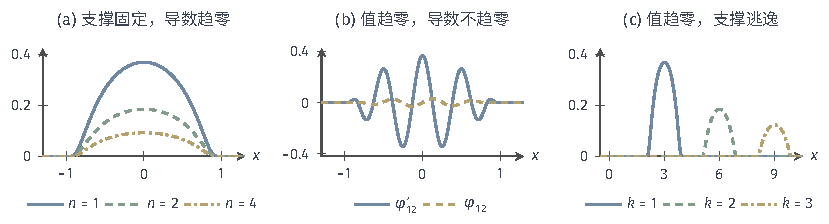
\includegraphics[width=140.4mm]{figures/02-abstract-mathematics/03-function-spaces/tikz/c4-test-sequences/figure.pdf}
  \caption{三列测试函数的对照。(a)~$\psi/n$：支撑固定在$[-1,1]$，函数值及各阶导数都一致趋零，这是测试意义下的趋零。(b)~$\varphi_n=\psi(x)\sin(nx)/n$，图中$n=12$：函数值（虚线）的上确界不超过$e^{-1}/12\approx0.031$，导数（实线）的上确界却约为$e^{-1}\approx0.37$，不随$n$减小。(c)~$\psi(x-3k)/k$：函数值和导数都一致趋零，支撑却跑向无穷远，不落在同一个紧集内。}
  \label{fig:sob-test-sequences}
\end{figure*}

第一列$\psi/n$的支撑固定，每一阶导数都是$D^\alpha\psi/n$，一致趋零；无论用什么合理的方式衡量，它都在变小。第二列$\varphi_n(x)=\psi(x)\sin(nx)/n$的函数值一致趋零，但
\[
 \varphi_n'(x)=\frac{\psi'(x)\sin(nx)}{n}+\psi(x)\cos(nx),
\]
第二项在原点等于$\psi(0)=e^{-1}$，导数并不变小。第三列$\psi(x-3k)/k$的函数值与各阶导数都一致趋零，但支撑向右逃逸，任何固定的紧集都装不下所有项。

后两列在测试意义下都不应算作趋零，因为确实存在合理的读数对它们给出不趋零的结果。读取原点导数的$\varphi\mapsto-\varphi'(0)$在第二列上恒为$-e^{-1}$；读数$\varphi\mapsto\sum_{k\ge1}k\,\varphi(3k)$在每个测试上只有有限项非零，因而有定义，它在第三列的第$k$项上取值$k\cdot\psi(0)/k=e^{-1}$。这两个读数都会在下面被确认为广义函数。于是测试的收敛必须同时控制支撑和所有阶导数：称$\varphi_n\to\varphi$（在测试意义下），若存在同一个紧集$K\subset\Omega$包含所有$\operatorname{supp}\varphi_n$与$\operatorname{supp}\varphi$，并且对每个多重指标$\alpha$都有$\sup_K|D^\alpha\varphi_n-D^\alpha\varphi|\to0$。这里的多重指标约定见第~\ref{sec:sob-distribution-derivative}节；在一维，$D^\alpha$就是$k$阶导数。

这一收敛不是由某一个范数给出的：上确界范数忽略导数，加入有限阶导数也挡不住更高阶的振荡，而支撑条件根本不是范数能表达的。完整的做法是在$C_c^\infty(\Omega)$上建立一种局部凸拓扑，本章不展开这一理论，只使用上面这个序列判据以及下一小节与之配套的估计。

\subsection{广义函数的定义与例子}
\label{sec:sob-distribution-def}

有了测试函数，我们把“对每个测试给出一个数”的对象作为新的研究对象。它应当是线性的，并且在每个固定的紧集上，读数受测试的有限阶导数的大小控制。

\begin{definition}[广义函数]
\label{def:sob-distribution}
称线性映射$T:C_c^\infty(\Omega)\to\mathbb F$为$\Omega$上的\term{广义函数}（generalized function，传统上称distribution），若对每个紧集$K\subset\Omega$，存在常数$C_K\ge0$和非负整数$m_K$，使所有支撑含于$K$的测试$\varphi$满足
\begin{equation}
 |T(\varphi)|\le C_K\sum_{|\alpha|\le m_K}\sup_K|D^\alpha\varphi| .
 \label{eq:sob-distribution-estimate}
\end{equation}
$\Omega$上广义函数的全体记作$\mathcal D'(\Omega)$。
\end{definition}

估计~\eqref{eq:sob-distribution-estimate}保证了上一小节要求的连续性：若$\varphi_n\to\varphi$（测试意义下），所有支撑落在同一个$K$内，对差$\varphi_n-\varphi$用这个估计，右端是有限多个一致趋零的量之和，所以$T(\varphi_n)\to T(\varphi)$。常数$C_K$与阶数$m_K$可以随紧集变化，这让广义函数在区域内部“越靠近边界越剧烈”也被允许。可以证明，反过来序列连续也推出这样的估计，因此两种说法等价；本章只用估计这一侧。广义函数作为线性泛函的观点，与第~\ref{sec:lfo-operators}节对有界线性泛函的讨论一致，区别在于这里的定义域$C_c^\infty(\Omega)$不是赋范空间，连续性只能逐个紧集表述。

\paragraph{由局部可积函数给出的广义函数}
对$f\in L^1_{\mathrm{loc}}(\Omega)$定义
\begin{equation}
 T_f(\varphi)=\int_\Omega f\varphi\,\mathrm dx .
 \label{eq:sob-regular-distribution}
\end{equation}
线性是显然的，估计~\eqref{eq:sob-local-pairing}正是$m_K=0$、$C_K=\int_K|f|$时的式~\eqref{eq:sob-distribution-estimate}，所以$T_f$是广义函数。几乎处处相等的$f$给出同一个$T_f$；下一节将证明反过来也成立，即$T_f=T_g$推出$f=g$几乎处处，于是可以把局部可积函数看作特殊的广义函数而不丢失信息。要强调的是，$T_f$读取的是$f$与测试的加权平均，并没有给$f$补上任何一点处的值：$1/x$在$(0,1)$上产生的广义函数，同样不回答“$f$在某点等于多少”。

\paragraph{点读数与测度}
不由普通函数给出的最简单例子是点读数。固定$x_0\in\Omega$，令
\[
 \delta_{x_0}(\varphi)=\varphi(x_0).
\]
它显然线性，并满足$|\delta_{x_0}(\varphi)|\le\sup_K|\varphi|$，取$m_K=0$、$C_K=1$即可，所以它是广义函数，称为\term{Dirac广义函数}（Dirac delta）。第~\ref{sec:sob-kinks-jumps}节将证明，不存在局部可积函数$g$使$\delta_{x_0}=T_g$。

点读数是测度积分的特例。设$\mu$是$\Omega$上的Borel测度，并且在每个紧集上取有限值（称为局部有限测度），令
\[
 T_\mu(\varphi)=\int_\Omega\varphi\,\mathrm d\mu ,\qquad |T_\mu(\varphi)|\le\mu(K)\sup_K|\varphi| .
\]
它也是$m_K=0$的广义函数。$\delta_{x_0}$对应集中在$x_0$的单位点质量，即第~\ref{sec:lfo-ck-dual}节的Dirac测度；上一小节的读数$\sum_{k\ge1}k\,\varphi(3k)$来自测度$\sum_kk\,\delta_{3k}$，每个紧集只含有限个质点，测度局部有限，所以它也是广义函数；$T_f$在$f\ge0$时对应以$f$为密度的测度$f\,\mathrm dx$，与第~\ref{sec:measure-same-space-comparison}节的Radon--Nikodym密度一致。允许测度带符号（在每个紧集上全变差有限）时，同样的估计以全变差$|\mu|(K)$代替$\mu(K)$。

这样，局部可积函数和局部有限测度都能产生广义函数，但广义函数比它们更宽。它不必是正的：若对所有非负测试都有$T(\varphi)\ge0$，称$T$为正的，$T_f$只在$f\ge0$几乎处处时才正。它也不必由测度给出：由测度给出的广义函数都满足$m_K=0$的估计，只受测试函数值的控制，而下一小节的$D\delta_0$需要读取测试的导数，将越出这一范围。

\subsection{广义函数的微分}
\label{sec:sob-distribution-derivative}

现在可以把导数转移到测试上。先约定多变量的记号。\term{多重指标}（multi-index）是非负整数组$\alpha=(\alpha_1,\ldots,\alpha_d)$，其阶数$|\alpha|=\alpha_1+\cdots+\alpha_d$，对应的偏导数
\[
 D^\alpha=\partial_1^{\alpha_1}\cdots\partial_d^{\alpha_d}.
\]
例如$d=2$、$\alpha=(1,2)$时，$D^\alpha=\partial_1\partial_2^2$，阶数为$3$；$\alpha=(0,\ldots,0)$时约定$D^\alpha$为恒等运算。测试函数的混合偏导数与求导次序无关，因此$D^\alpha$的定义没有歧义。

对$f\in C^{|\alpha|}(\Omega)$和测试$\varphi$，把式~\eqref{eq:sob-integration-by-parts}逐坐标重复$|\alpha|$次，每转移一次导数产生一个负号，测试的紧支撑使每一步都没有边界项：
\begin{equation}
 \int_\Omega(D^\alpha f)\,\varphi\,\mathrm dx=(-1)^{|\alpha|}\int_\Omega f\,D^\alpha\varphi\,\mathrm dx .
 \label{eq:sob-repeated-parts}
\end{equation}
用广义函数的语言，左端是$T_{D^\alpha f}(\varphi)$，右端是$(-1)^{|\alpha|}T_f(D^\alpha\varphi)$。右端对任何广义函数都有意义，于是取它作为定义。

\begin{definition}[广义导数]
\label{def:sob-distribution-derivative}
设$T\in\mathcal D'(\Omega)$，$\alpha$为多重指标。定义$T$的$\alpha$阶\term{广义导数}（distributional derivative）为
\begin{equation}
 (D^\alpha T)(\varphi)=(-1)^{|\alpha|}\,T(D^\alpha\varphi),\qquad\varphi\in C_c^\infty(\Omega).
 \label{eq:sob-distribution-derivative}
\end{equation}
\end{definition}

我们需要核对$D^\alpha T$仍是广义函数。线性由$T$和$D^\alpha$的线性得到。对支撑含于$K$的测试，$D^\alpha\varphi$的支撑也在$K$内，代入$T$的估计，
\[
 |(D^\alpha T)(\varphi)|\le C_K\sum_{|\beta|\le m_K}\sup_K|D^{\beta}D^\alpha\varphi|
 \le C_K\sum_{|\gamma|\le m_K+|\alpha|}\sup_K|D^\gamma\varphi| ,
\]
所以$D^\alpha T$满足阶数为$m_K+|\alpha|$的估计。由此得到三条基本性质。其一，每个广义函数都可以求任意阶导数，导数仍是广义函数，这与经典导数截然不同。其二，由式~\eqref{eq:sob-repeated-parts}，当$f\in C^{|\alpha|}(\Omega)$时$D^\alpha T_f=T_{D^\alpha f}$，新定义与经典导数相容。其三，因为测试的混合偏导数可交换，$D^\alpha D^\beta T=D^{\alpha+\beta}T$，广义导数的次序也无关紧要。

\paragraph{点读数的导数}
看最简单的非函数对象。在实轴上，按定义
\[
 (D\delta_0)(\varphi)=-\delta_0(\varphi')=-\varphi'(0).
\]
$D\delta_0$读取测试在原点的导数并反号，它满足$m_K=1$的估计$|(D\delta_0)(\varphi)|\le\sup_K|\varphi'|$。直观地说，$\delta_0$是集中在原点的单位质量，$D\delta_0$则像在原点两侧紧挨着放置一正一负两个质量所形成的“偶极子”。

$D\delta_0$不能由任何测度给出，下面用固定支撑、函数值有界而原点导数无界的测试来说明。

\begin{example}[$D\delta_0$不是测度]
\label{ex:sob-ddelta-not-measure}
设有实轴上的带符号Borel测度$\mu$，在紧集上全变差有限，并且$D\delta_0=T_\mu$。取光滑截断$\chi$，使其在$[-0.3,0.3]$上为$1$、支撑在$[-0.9,0.9]$内（例如图~\ref{fig:sob-bump-cutoff}(b)中的函数），令
\[
 \varphi_n(x)=\chi(x)\sin(nx).
\]
每个$\varphi_n$的支撑都在$K=[-0.9,0.9]$内，且$|\varphi_n|\le1$。由于$\chi$在原点附近恒为$1$，$\varphi_n'(0)=n\cos0=n$。一方面$|T_\mu(\varphi_n)|\le|\mu|(K)\sup|\varphi_n|\le|\mu|(K)$；另一方面$|(D\delta_0)(\varphi_n)|=|\varphi_n'(0)|=n$。令$n\to\infty$即得矛盾。图~\ref{fig:sob-ddelta-test}画出$n=3$与$n=10$的测试及其原点切线。
\end{example}

\begin{figure}[!htb]
  \centering
  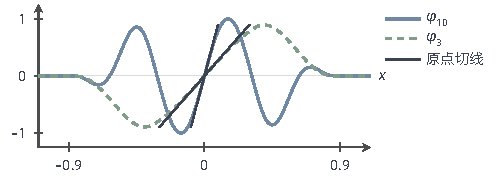
\includegraphics[width=84.4mm]{figures/02-abstract-mathematics/03-function-spaces/tikz/c4-ddelta-test/figure.pdf}
  \caption{区分$D\delta_0$与测度的测试$\varphi_n(x)=\chi(x)\sin(nx)$，$n=3$（虚线）与$n=10$（实线）。两者的支撑都在$[-0.9,0.9]$内，函数值都不超过$1$，测度的读数因而一致有界；原点处的切线斜率却等于$n$，$D\delta_0$的读数$-\varphi_n'(0)=-n$随$n$无界。}
  \label{fig:sob-ddelta-test}
\end{figure}

这个例子与上一小节图~\ref{fig:sob-test-sequences}(b)是同一个机制：只控制函数值不能控制导数的读数。它说明广义函数严格大于测度，求导会把函数（甚至测度）推出原来的对象类型。于是自然要问：从一个局部可积函数出发，它的广义导数什么时候仍然是一个局部可积函数？这正是下一节要回答的问题。

% 第4章第2节：弱导数与经典微分（弱导数的定义与唯一性、尖点跳跃与奇异变化、一维弱导数与绝对连续性）。

\section{弱导数与经典微分}
\label{sec:sob-weak-derivatives}

上一节说明，任何局部可积函数$f$都有各阶广义导数$D^\alpha T_f$，但它们可能是$\delta_0$这样的点读数，甚至连测度都不是。本节固定$f\in L^1_{\mathrm{loc}}(\Omega)$，研究一个更具体的问题：$D^\alpha T_f$什么时候仍由一个局部可积函数给出。我们先给出定义并证明这样的函数在几乎处处意义下唯一，再用尖点、跳跃和Cantor函数比较三种不同的结局，最后在一维情形证明，这个条件恰好等价于函数有绝对连续的代表。

\subsection{弱导数的定义与唯一性}
\label{sec:sob-weak-derivative-def}

若广义导数$D^\alpha T_f$等于某个$T_g$，按式~\eqref{eq:sob-distribution-derivative}与式~\eqref{eq:sob-regular-distribution}展开，就是对所有测试成立一个积分恒等式。我们把这个恒等式直接作为定义。

\begin{definition}[弱导数]
\label{def:sob-weak-derivative}
设$f,g\in L^1_{\mathrm{loc}}(\Omega)$，$\alpha$为多重指标。若对所有$\varphi\in C_c^\infty(\Omega)$都有
\begin{equation}
 \int_\Omega g\,\varphi\,\mathrm dx=(-1)^{|\alpha|}\int_\Omega f\,D^\alpha\varphi\,\mathrm dx ,
 \label{eq:sob-weak-derivative}
\end{equation}
则称$g$为$f$的$\alpha$阶\term{弱导数}（weak derivative），记作$D^\alpha f=g$。一阶情形也写作$\partial_jf$，全部一阶弱导数组成的向量记作弱梯度$\nabla f$。
\end{definition}

与广义导数相比，这里多了一个实质性的条件：存在一个局部可积函数$g$来表示$D^\alpha T_f$。广义导数总存在，弱导数却未必。恒等式必须对\emph{所有}测试成立，只在若干个测试上核对是不够的；也不能用“经典导数几乎处处存在”来代替它，第~\ref{sec:sob-kinks-jumps}节的阶跃和Cantor函数会说明这一点。由式~\eqref{eq:sob-repeated-parts}，$C^{|\alpha|}$函数的经典导数就是弱导数，所以这一定义推广了经典导数。

\paragraph{运算规则}
弱导数对$f$是线性的：若$D^\alpha f_1=g_1$，$D^\alpha f_2=g_2$，则对标量$a,b$有$D^\alpha(af_1+bf_2)=ag_1+bg_2$，因为恒等式~\eqref{eq:sob-weak-derivative}两边都对$f$和$g$线性。与光滑函数相乘也有乘积法则。设$a\in C^\infty(\Omega)$，$f$有一阶弱导数$\partial_jf$。对任意测试$\varphi$，$a\varphi$仍是测试，且$\partial_j(a\varphi)=a\,\partial_j\varphi+\varphi\,\partial_ja$，于是
\[
 \int_\Omega af\,\partial_j\varphi\,\mathrm dx
 =\int_\Omega f\,\partial_j(a\varphi)\,\mathrm dx-\int_\Omega f\varphi\,\partial_ja\,\mathrm dx
 =-\int_\Omega\bigl(a\,\partial_jf+f\,\partial_ja\bigr)\varphi\,\mathrm dx ,
\]
第二个等号对测试$a\varphi$使用了弱导数的定义。右端括号内的函数局部可积，所以$\partial_j(af)=a\,\partial_jf+f\,\partial_ja$。

两个都弱可微的函数相乘则要另查可积性。在$\mathbb R^3$中取$f(x)=|x|^{-6/5}$。它在原点外光滑，$|\nabla f|=\frac65|x|^{-11/5}$；由上一节的幂函数阈值，$f$与$|\nabla f|$都局部可积（$6/5<3$，$11/5<3$），用挖去小球再令半径趋零的分部积分可以验证$\nabla f$确实是弱梯度。可是乘积法则给出的候选$2f\nabla f$大小为$\frac{12}{5}|x|^{-17/5}$，指数$17/5>3$，不局部可积。因此$f^2=|x|^{-12/5}$虽然局部可积，却没有局部可积的弱梯度。乘积法则只在各项可积时才能使用。

\paragraph{测试函数区分局部可积函数}
为了说明弱导数确定到几乎处处，我们先证明一条更基本的事实：如果一个局部可积函数与所有测试的配对都为零，它本身几乎处处为零。证明需要Lebesgue测度的两条正则性：对正测度的可测集$A$，存在紧集$C\subset A$且$|C|>0$（内正则性）；对任意可测集$C$和$\eta>0$，存在开集$U\supset C$使$|U\setminus C|<\eta$（外正则性）。这里$|\cdot|$表示Lebesgue测度。外正则性来自用可数个开盒子覆盖来定义Lebesgue外测度的方式，内正则性可由外正则性对补集使用得到。证明还要用到积分的绝对连续性：若$h$在集合$E_0$上可积，则对任意$\eta>0$，存在$\delta>0$，使$E_0$中测度小于$\delta$的子集$E$都满足$\int_E|h|<\eta$。

\begin{lemma}[测试函数区分局部可积函数]
\label{lem:sob-fundamental}
设$h\in L^1_{\mathrm{loc}}(\Omega)$，且对所有$\varphi\in C_c^\infty(\Omega)$都有$\int_\Omega h\varphi\,\mathrm dx=0$。则$h=0$几乎处处。
\end{lemma}

\begin{proof}
复值时分别处理实部和虚部（实值测试的配对分别给出两者的配对），所以只需考虑实值$h$。反设$h$不几乎处处为零，则$\{h>0\}$或$\{h<0\}$有正测度；以$-h$代替$h$，不妨设$\{h>0\}$有正测度。

第一步，找一块有正积分的紧集。令$G_m=\{x\in\Omega:|x|<m,\ \operatorname{dist}(x,\partial\Omega)>1/m\}$（$\Omega=\mathbb R^d$时只要求$|x|<m$），它们是递增的开集，闭包紧且含于$\Omega$，并集为$\Omega$。由可数可加性，某个$A=\{h>0\}\cap G_m$有正测度。内正则性给出紧集$C\subset A$且$|C|>0$；$h$在$C$上为正，所以$a:=\int_Ch\,\mathrm dx>0$。

第二步，用截断控制外侧误差。$h$在紧集$\overline{G_{m+1}}$上可积，由积分的绝对连续性，取$\delta>0$使$\overline{G_{m+1}}$中测度小于$\delta$的集合$E$满足$\int_E|h|<a/2$。外正则性给出开集$U'\supset C$且$|U'\setminus C|<\delta$；令$U=U'\cap G_{m+1}$，它仍是包含$C$的开集。由引理~\ref{lem:sob-cutoff}，取$\chi\in C_c^\infty(U)$，$0\le\chi\le1$，在$C$上$\chi=1$。

第三步，计算配对。因为$\chi$在$C$上为$1$，在$U$外为$0$，
\[
 \int_\Omega h\chi\,\mathrm dx=\int_Ch\,\mathrm dx+\int_{U\setminus C}h\chi\,\mathrm dx
 \ge a-\int_{U\setminus C}|h|\,\mathrm dx>a-\frac a2>0 ,
\]
与假设$\int h\chi=0$矛盾。所以$h=0$几乎处处。
\end{proof}

这条引理的证明只用了截断函数和测度的正则性，没有借助后面的平滑逼近定理。它的作用是说明：测试函数足够多，能够把局部可积函数的等价类彼此分开。直接的推论是映射$f\mapsto T_f$是单射：$T_f=T_g$意味着$f-g$与所有测试的配对为零，从而$f=g$几乎处处。

\begin{theorem}[弱导数的唯一性]
\label{thm:sob-weak-derivative-unique}
设$f\in L^1_{\mathrm{loc}}(\Omega)$。若$g_1,g_2\in L^1_{\mathrm{loc}}(\Omega)$都是$f$的$\alpha$阶弱导数，则$g_1=g_2$几乎处处。
\end{theorem}

\begin{proof}
两个恒等式~\eqref{eq:sob-weak-derivative}的右端相同，相减得$\int(g_1-g_2)\varphi=0$对所有测试成立，由引理~\ref{lem:sob-fundamental}即得结论。
\end{proof}

唯一的是等价类：改变$g$在零测集上的值不破坏恒等式，所以“弱导数在某一点的值”没有意义，正如$L^p$元素在一点的值没有意义一样。

\subsection{尖点、跳跃与奇异变化}
\label{sec:sob-kinks-jumps}

现在比较三个在单点或零测集上“出问题”的函数。它们都几乎处处有经典导数，却分别落在三种不同的结局里。

\paragraph{尖点：$|x|$}
在实轴上取$f(x)=|x|$。对测试$\varphi$，在原点两侧分别分部积分：
\[
\begin{aligned}
 \int_{-\infty}^{\infty}|x|\varphi'(x)\,\mathrm dx
 &=\int_{-\infty}^0(-x)\varphi'(x)\,\mathrm dx+\int_0^\infty x\varphi'(x)\,\mathrm dx\\
 &=\Bigl[-x\varphi(x)\Bigr]_{-\infty}^{0}+\int_{-\infty}^0\varphi\,\mathrm dx
 +\Bigl[x\varphi(x)\Bigr]_{0}^{\infty}-\int_0^\infty\varphi\,\mathrm dx\\
 &=-\int_{-\infty}^{\infty}\operatorname{sgn}(x)\,\varphi(x)\,\mathrm dx .
\end{aligned}
\]
四个边界项都为零：在$\pm\infty$一侧，测试紧支撑；在原点一侧，因子$x$等于零。这正是式~\eqref{eq:sob-weak-derivative}在$\alpha=1$、$g=\operatorname{sgn}x$时的形式，所以$|x|$的弱导数是$\operatorname{sgn}x$（图~\ref{fig:sob-abs-sign}）。原点的经典导数不存在，但这只涉及一个零测点；$\operatorname{sgn}0$取什么值都不影响结论。

\begin{figure}[!htb]
  \centering
  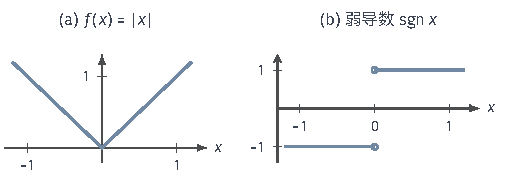
\includegraphics[width=85.7mm]{figures/02-abstract-mathematics/03-function-spaces/tikz/c4-abs-sign/figure.pdf}
  \caption{尖点函数与它的弱导数。(a)~$f(x)=|x|$在原点连续但有尖点；(b)~弱导数$\operatorname{sgn}x$在原点两侧分别为$-1$与$1$，空心点表示原点的取值可以任意约定，弱导数作为等价类不受影响。}
  \label{fig:sob-abs-sign}
\end{figure}

边界项在原点相消，靠的是$|x|$在原点连续。下面的阶跃函数在原点断开，同样的计算会留下一个点读数。

\paragraph{跳跃：阶跃函数}
取$H=\mathbf 1_{(0,\infty)}$。对测试$\varphi$，
\[
 (DT_H)(\varphi)=-\int_{-\infty}^{\infty}H\varphi'\,\mathrm dx=-\int_0^\infty\varphi'\,\mathrm dx=\varphi(0),
\]
所以$DT_H=\delta_0$。$H$在原点外处处可导且经典导数为零，但零函数不是它的弱导数：$\int0\cdot\varphi=0$，而$\delta_0(\varphi)=\varphi(0)$对$\varphi(0)\neq0$的测试不为零。跳跃把变化全部集中在一点上，留下的是测试在跳点的取值。

还要说明$\delta_0$不能由\emph{任何}局部可积函数表示，这样$H$才确实没有弱导数。

\begin{example}[$\delta_0$不是局部可积函数]
\label{ex:sob-delta-not-function}
反设$g\in L^1_{\mathrm{loc}}(\mathbb R)$使$\delta_0=T_g$。取图~\ref{fig:sob-bump-cutoff}(b)中的截断$\chi$，令$\varphi_\varepsilon(x)=\chi(x/\varepsilon)$，$0<\varepsilon\le1$。每个$\varphi_\varepsilon$满足$0\le\varphi_\varepsilon\le1$、$\varphi_\varepsilon(0)=1$，支撑在$[-\varepsilon,\varepsilon]$内（图~\ref{fig:sob-step-delta}(b)）。于是
\[
 1=\delta_0(\varphi_\varepsilon)=\int g\varphi_\varepsilon\,\mathrm dx,\qquad
 \left|\int g\varphi_\varepsilon\,\mathrm dx\right|\le\int_{-\varepsilon}^{\varepsilon}|g|\,\mathrm dx .
\]
$g$在$[-1,1]$上可积，区间$[-\varepsilon,\varepsilon]$的测度趋于零，由积分的绝对连续性，右端趋于零，与左端恒为$1$矛盾。
\end{example}

\begin{figure}[!htb]
  \centering
  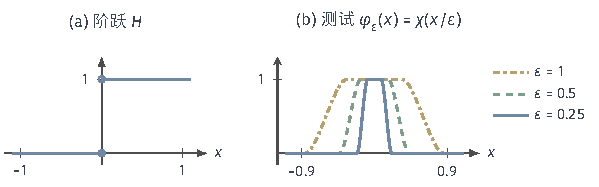
\includegraphics[width=101.5mm]{figures/02-abstract-mathematics/03-function-spaces/tikz/c4-step-delta/figure.pdf}
  \caption{跳跃留下点读数。(a)~阶跃$H=\mathbf 1_{(0,\infty)}$，其广义导数为$\delta_0$。(b)~支撑缩小的测试$\varphi_\varepsilon(x)=\chi(x/\varepsilon)$，$\varepsilon=1,0.5,0.25$：原点值始终为$1$，因此$\delta_0$的读数恒为$1$；而任何局部可积函数与$\varphi_\varepsilon$的配对都被它在越来越短区间上的积分控制，趋于零。}
  \label{fig:sob-step-delta}
\end{figure}

图~\ref{fig:sob-step-delta}把两种读数的差别画了出来：点读数只看原点，测试缩得再窄，读数也不变；函数的积分读数却要乘上支撑的宽度，最终消失。顺带可知$\operatorname{sgn}x=2H-1$的广义导数是$2\delta_0$，所以$|x|$有一阶弱导数，却没有二阶弱导数。

\paragraph{奇异连续变化：Cantor函数}
跳跃的变化集中在一点，函数因而不连续。是否连续函数、且经典导数几乎处处存在，就一定有弱导数？Cantor函数给出否定的回答。

回顾它的构造。从$[0,1]$出发，挖去中间三分之一的开区间$(1/3,2/3)$，在其上令$c=1/2$；对剩下的两个闭区间各自挖去中间三分之一，在$(1/9,2/9)$上令$c=1/4$，在$(7/9,8/9)$上令$c=3/4$；如此继续，第$m$步挖去$2^{m-1}$个长为$3^{-m}$的开区间，并在其上分别取相邻两层平台值的平均。被挖去区间的总长度为$\sum_{m\ge1}2^{m-1}3^{-m}=1$，剩下的Cantor集测度为零。再令$c(0)=0$、$c(1)=1$，并在Cantor集上按单调性补齐，得到$[0,1]$上连续、单调不减的函数$c$（图~\ref{fig:sob-cantor}(a)）。它在每个被挖去的开区间上为常数，所以在测度为$1$的集合上经典导数为零。以概率的语言说，$c$是一个随机变量的分布函数，这个随机变量没有任何单点概率，也没有密度；这一观察可参考\BookChapterRef{chap:random-variables}{卷一“随机变量与概率分布”章}。

\begin{figure}[!htb]
  \centering
  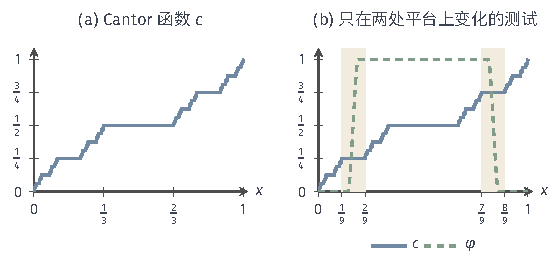
\includegraphics[width=94.7mm]{figures/02-abstract-mathematics/03-function-spaces/tikz/c4-cantor/figure.pdf}
  \caption{Cantor函数没有弱导数。(a)~$c$连续、单调，在被挖去的区间$(\frac13,\frac23)$、$(\frac19,\frac29)$、$(\frac79,\frac89)$等上为常数，在测度为$1$的集合上经典导数为零。(b)~测试$\varphi$（虚线）只在阴影区间$(\frac19,\frac29)$与$(\frac79,\frac89)$内变化，那里$c$分别为$\frac14$与$\frac34$，于是$-\int c\varphi'=-\frac14+\frac34=\frac12$；若$c$有弱导数，这个读数必须为零。}
  \label{fig:sob-cantor}
\end{figure}

\begin{example}[Cantor函数没有弱导数]
\label{ex:sob-cantor}
反设$c$在$(0,1)$上有弱导数$g\in L^1_{\mathrm{loc}}(0,1)$。先在每个被挖去的开区间$I$上看：对支撑在$I$内的测试$\varphi$，$c$在$I$上为常数$c_I$，所以
\[
 \int_Ig\varphi\,\mathrm dx=-\int_Ic_I\,\varphi'\,\mathrm dx=0 .
\]
对开集$I$使用引理~\ref{lem:sob-fundamental}，得$g=0$在$I$上几乎处处成立。被挖去的区间可数个，总长为$1$，因此$g=0$在$(0,1)$上几乎处处成立，从而对所有测试都应有$\int c\varphi'=-\int g\varphi=0$。

再取一个具体测试：$\varphi$在$(1/9,2/9)$内由$0$光滑地升到$1$，在$[2/9,7/9]$上恒为$1$，在$(7/9,8/9)$内光滑地降到$0$（图~\ref{fig:sob-cantor}(b)）。$\varphi'$只在这两个区间内非零，而$c$在那里分别等于$1/4$和$3/4$，所以
\[
 \begin{aligned}
 -\int_0^1c\,\varphi'\,\mathrm dx
 &=-\frac14\int_{1/9}^{2/9}\varphi'\,\mathrm dx-\frac34\int_{7/9}^{8/9}\varphi'\,\mathrm dx\\
 &=-\frac14\cdot1-\frac34\cdot(-1)=\frac12\neq0 ,
 \end{aligned}
\]
矛盾。所以$c$没有弱导数。
\end{example}

读数$1/2$正好是$c$在$[2/9,7/9]$上的增量。实际上，$c$的广义导数是$c$所对应的Lebesgue--Stieltjes测度$\mu_c$（由$\mu_c((s,t])=c(t)-c(s)$确定），它集中在测度为零的Cantor集上，相对Lebesgue测度是奇异的；按第~\ref{sec:measure-lebesgue-decomposition}节的Lebesgue分解（定理~\ref{thm:measure-lebesgue-decomposition}），它没有绝对连续部分，因而不能写成$g\,\mathrm dx$。

\paragraph{三个例子的对照}
表~\ref{tab:sob-three-examples}把三个函数放在一起。三者都几乎处处有经典导数，广义导数也都存在，区别在于广义导数是什么类型的对象。只有$|x|$的广义导数是局部可积函数，才有弱导数；阶跃的变化集中成点质量，Cantor函数的变化集中成奇异连续测度。所以“几乎处处可微”与“弱可微”是两回事：前者只看测度为$1$的集合上的局部斜率，后者要求整体的积分恒等式成立。

\begin{table}[!htb]
 \centering
 \caption{尖点、跳跃与奇异连续变化的对照（区间$(-1,1)$或$(0,1)$上）。}
 \label{tab:sob-three-examples}
 \begin{tabular}{@{}llll@{}}
  \toprule
  函数 & 经典导数 & 广义导数 & 有无弱导数\\
  \midrule
  $|x|$ & 除原点外为$\operatorname{sgn}x$ & $T_{\operatorname{sgn}}$ & 有，$\operatorname{sgn}x$\\
  $H=\mathbf 1_{(0,\infty)}$ & 除原点外为$0$ & $\delta_0$ & 无\\
  Cantor函数$c$ & 几乎处处为$0$ & 奇异测度$\mu_c$ & 无\\
  \bottomrule
 \end{tabular}
\end{table}

$|x|$与另两者的差别在于，它能由自己的导数积分恢复：$|x|=|x_0|+\int_{x_0}^x\operatorname{sgn}t\,\mathrm dt$。阶跃和Cantor函数都做不到这一点，因为它们的经典导数积分出来恒为零。下一小节证明，在一维情形，“能由导数积分恢复”恰好就是弱可微的含义。

\subsection{一维弱导数与绝对连续性}
\label{sec:sob-absolute-continuity}

本小节在有限区间$(a,b)$上工作，记长度$L=b-a$。我们先证明弱导数为零的函数是常数，再借此把弱导数与积分表示联系起来。

\begin{lemma}[弱导数为零的函数]
\label{lem:sob-zero-derivative}
设$f\in L^1_{\mathrm{loc}}(a,b)$，且$\int_a^bf\varphi'\,\mathrm dx=0$对所有$\varphi\in C_c^\infty(a,b)$成立。则存在常数$c$，使$f=c$几乎处处。
\end{lemma}

\begin{proof}
关键是看出哪些测试能写成另一个测试的导数。若$\psi\in C_c^\infty(a,b)$且$\int\psi=0$，则$\varphi(x)=\int_a^x\psi(t)\,\mathrm dt$是光滑的；在$\operatorname{supp}\psi$左侧$\varphi=0$，在其右侧$\varphi=\int\psi=0$，所以$\varphi\in C_c^\infty(a,b)$且$\varphi'=\psi$。于是假设给出：$f$与每个积分为零的测试配对为零。

固定一个积分为$1$的测试$\theta$（例如平移伸缩后的$\rho_\varepsilon$）。任意测试$\psi$可写成$\psi=\bigl(\int\psi\bigr)\theta+\bigl(\psi-(\int\psi)\theta\bigr)$，后一项积分为零，与$f$的配对为零。所以
\[
 \int_a^bf\psi\,\mathrm dx=\Bigl(\int_a^b\psi\,\mathrm dx\Bigr)\int_a^bf\theta\,\mathrm dx=\int_a^bc\,\psi\,\mathrm dx,\qquad c=\int_a^bf\theta\,\mathrm dx .
\]
即$f-c$与所有测试的配对为零，由引理~\ref{lem:sob-fundamental}，$f=c$几乎处处。
\end{proof}

接下来需要一维实分析中的绝对连续函数。称$F:[a,b]\to\mathbb F$\term{绝对连续}（absolutely continuous），若对任意$\varepsilon>0$存在$\delta>0$，使对$[a,b]$中任意有限个两两不交的子区间$(x_i,y_i)$，只要$\sum_i(y_i-x_i)<\delta$，就有$\sum_i|F(y_i)-F(x_i)|<\varepsilon$。它比一致连续强：一致连续只控制一个短区间上的增量，绝对连续控制总长度很短的许多区间上增量之和。Cantor函数连续却不绝对连续：第$m$步剩下$2^m$个闭区间，总长$(2/3)^m$可以任意小，$c$在它们上的增量之和却始终为$1$。

下面使用Lebesgue关于绝对连续函数的微积分基本定理，不在这里证明：若$g\in L^1(a,b)$，则$G(x)=\int_a^xg(t)\,\mathrm dt$在$[a,b]$上绝对连续，且$G'=g$几乎处处；反过来，若$F$在$[a,b]$上绝对连续，则$F$几乎处处可导，$F'\in L^1(a,b)$，并且$F(x)=F(a)+\int_a^xF'(t)\,\mathrm dt$。当$F$单调不减时，这正是说$F$对应的Lebesgue--Stieltjes测度相对Lebesgue测度绝对连续，$F'$是Radon--Nikodym密度（定理~\ref{thm:density-radon-nikodym}）；Cantor函数的测度则完全奇异。

\begin{theorem}[一维弱导数与绝对连续代表]
\label{thm:sob-1d-absolute-continuity}
设$f,g\in L^1(a,b)$。则$g$是$f$的弱导数，当且仅当$f$有一个绝对连续的代表$\tilde f$，满足
\begin{equation}
 \tilde f(y)-\tilde f(x)=\int_x^yg(t)\,\mathrm dt,\qquad a\le x\le y\le b .
 \label{eq:sob-1d-integral-representation}
\end{equation}
此时$\tilde f$在$[a,b]$上唯一，几乎处处有经典导数$\tilde f'=g$。
\end{theorem}

\begin{proof}
先证明累积积分$G(x)=\int_a^xg(t)\,\mathrm dt$以$g$为弱导数。对测试$\varphi$，
\[
 \begin{aligned}
 \int_a^bG\varphi'\,\mathrm dx&=\int_a^b\!\!\int_a^b\mathbf 1_{\{t<x\}}\,g(t)\varphi'(x)\,\mathrm dt\,\mathrm dx\\
 &=\int_a^bg(t)\Bigl(\int_t^b\varphi'(x)\,\mathrm dx\Bigr)\mathrm dt=-\int_a^bg\varphi\,\mathrm dt .
 \end{aligned}
\]
交换积分次序的依据是Fubini定理：被积函数的绝对值不超过$|g(t)|\sup|\varphi'|$，在正方形$[a,b]^2$上可积。最后一步用了$\varphi(b)=0$。

必要性。若$g$是$f$的弱导数，则$f-G$的弱导数为零，由引理~\ref{lem:sob-zero-derivative}，存在常数$c$使$f=c+G$几乎处处。$\tilde f=c+G$绝对连续，并满足式~\eqref{eq:sob-1d-integral-representation}。

充分性。若$f$有满足式~\eqref{eq:sob-1d-integral-representation}的代表，取$x=a$得$\tilde f=\tilde f(a)+G$，常数的弱导数为零，所以$f$的弱导数就是$G$的弱导数$g$。

唯一性：两个连续代表几乎处处相等，在区间的每个非空开子集上不可能处处不同，因而处处相等（非空开区间的Lebesgue测度为正）。$\tilde f'=g$几乎处处来自上面引用的Lebesgue定理。
\end{proof}

定理把一维弱可微性完全翻译成了经典语言：有弱导数，就是能从导数积分回来。把条件放宽到$f,g\in L^1_{\mathrm{loc}}(a,b)$时，同样的论证给出一个在每个紧子区间上绝对连续的代表，只是它可能在端点附近无界，例如$(0,1)$上$f(x)=\ln x$，弱导数$1/x$局部可积但不可积。

\paragraph{积分指数给出Hölder控制}
若进一步知道$g\in L^p(a,b)$，式~\eqref{eq:sob-1d-integral-representation}还能定量地控制$\tilde f$的振荡。对$1<p<\infty$，设$q$为共轭指数，$1/p+1/q=1$。由Hölder不等式，
\begin{equation}
 |\tilde f(y)-\tilde f(x)|\le\int_x^y|g|\cdot1\,\mathrm dt\le\|g\|_{L^p}\,|y-x|^{1/q}=\|g\|_{L^p}\,|y-x|^{1-1/p} .
 \label{eq:sob-1d-holder}
\end{equation}
称满足$|F(x)-F(y)|\le M|x-y|^\gamma$的函数为$\gamma$阶\term{Hölder连续}（Hölder continuous），$0<\gamma\le1$；$\gamma=1$即Lipschitz连续。式~\eqref{eq:sob-1d-holder}说明$\tilde f$是$1-1/p$阶Hölder连续的，指数随$p$增大而增大；$p=\infty$时直接得到Lipschitz控制$|\tilde f(y)-\tilde f(x)|\le\|g\|_{L^\infty}|y-x|$。图~\ref{fig:sob-holder-1d}(a)画出了几种控制函数$h^{1-1/p}$。

\begin{figure}[!htb]
  \centering
  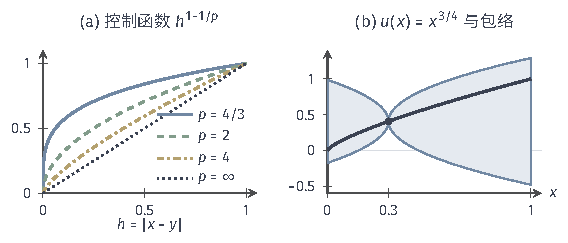
\includegraphics[width=96.2mm]{figures/02-abstract-mathematics/03-function-spaces/tikz/c4-holder-1d/figure.pdf}
  \caption{导数的积分指数控制函数的振荡。(a)~控制函数$h^{1-1/p}$，$p=4/3,2,4,\infty$对应Hölder指数$\frac14,\frac12,\frac34,1$；指数越小，短距离上允许的变化越大。(b)~$u(x)=x^{3/4}$的弱导数$\frac34x^{-1/4}$属于$L^2(0,1)$，$\|u'\|_{L^2}=\sqrt{9/8}\approx1.061$；由式~\eqref{eq:sob-1d-holder}，$u$的图像必须留在以$(0.3,u(0.3))$为顶点的阴影包络$u(0.3)\pm1.061|x-0.3|^{1/2}$内。}
  \label{fig:sob-holder-1d}
\end{figure}

图~\ref{fig:sob-holder-1d}(b)用一个具体函数检验这一估计。$u(x)=x^{3/4}$在原点的经典导数无界，但$u'(x)=\frac34x^{-1/4}$满足$\int_0^1|u'|^2=\frac9{16}\int_0^1x^{-1/2}\,\mathrm dx=\frac98$，所以$u'\in L^2(0,1)$；按定理~\ref{thm:sob-1d-absolute-continuity}它就是弱导数。取$p=2$，式~\eqref{eq:sob-1d-holder}说明$u$的图像整条落在以任一点为顶点、开口为$\sqrt{9/8}\,|x-y|^{1/2}$的包络内，图中以$y=0.3$为例。

$p=1$是例外：此时仍有绝对连续代表，却没有任何正的Hölder指数保证。例如在$(0,1/2)$上取$f(x)=1/\ln(1/x)$，并令$f(0)=0$。它单调增加，$f'(x)=1/\bigl(x\ln^2(1/x)\bigr)$，$\int_0^{1/2}f'=f(1/2)-f(0^+)=1/\ln2$有限，所以$f'\in L^1$。但对任意$\gamma>0$，$h^\gamma\ln(1/h)\to0$（$h\to0^+$），即$f(h)-f(0)=1/\ln(1/h)$比$h^\gamma$大得多，$f$在原点不满足任何正阶Hölder条件。

\paragraph{点值与端点值}
上面的估计还给出用$L^p$大小控制点值的方法。设$f,g\in L^p(a,b)$，$1\le p<\infty$。若$|\tilde f|$处处大于$L^{-1/p}\|f\|_{L^p}$，则$\int|\tilde f|^p>L\cdot L^{-1}\|f\|_{L^p}^p$，矛盾；所以存在$y\in[a,b]$使$|\tilde f(y)|\le L^{-1/p}\|f\|_{L^p}$。对任意$x\in[a,b]$，再由式~\eqref{eq:sob-1d-holder}（$p=1$时直接用$\int|g|$），
\begin{equation}
 \sup_{x\in[a,b]}|\tilde f(x)|\le L^{-1/p}\|f\|_{L^p}+L^{1-1/p}\|g\|_{L^p} .
 \label{eq:sob-1d-sup-bound}
\end{equation}
$p=2$时右端是$L^{-1/2}\|f\|_{L^2}+L^{1/2}\|g\|_{L^2}$。这个估计对闭区间的每一点同时成立，端点也包括在内。

要强调的是，这里的点值都是指唯一的连续代表$\tilde f$的值。在等价类中任取另一个代表，它可以在任意一个零测集上改值，点值便失去意义；正是弱导数的存在，从等价类中选出了唯一一个连续成员。这一结论依赖于一维：在高维，即使函数和全部一阶弱导数都平方可积，函数也可能在一点附近无界，第~\ref{sec:sob-embedding}节将看到维数和积分指数怎样共同决定连续代表是否存在。

% 第4章第3节：Sobolev空间（成员条件与范数、弱微分的定义域、完备性与Hilbert结构）。

\section{Sobolev空间}
\label{sec:sob-spaces}

弱导数的存在只回答了输出是什么类型的对象，还没有限制函数和导数有多大。$|x|$在整条实轴上有弱导数$\operatorname{sgn}x$，可两者都不可积；$\sin(nx)$的导数是$n\cos(nx)$，函数大小不变而导数随$n$无界。要把“变化受控”变成可以计算误差、取极限的条件，需要把函数和它的各阶弱导数一起放进范数。本节建立这样的空间，并证明极限过程中导数关系不会丢失。

\subsection{成员条件与Sobolev范数}
\label{sec:sob-norms}

我们希望同时控制函数本身和它直到某一阶的全部弱导数，并以$L^p$范数衡量每一项。

\begin{definition}[Sobolev空间]
\label{def:sob-sobolev-space}
设$\Omega\subset\mathbb R^d$为开集，$k\ge0$为整数，$1\le p<\infty$。称
\[
 W^{k,p}(\Omega)=\bigl\{u\in L^p(\Omega):\ \text{对每个}|\alpha|\le k,\ D^\alpha u\text{ 存在且属于 }L^p(\Omega)\bigr\}
\]
为\term{Sobolev空间}（Sobolev space），其中$D^0u=u$，并赋以\term{Sobolev范数}（Sobolev norm）
\begin{equation}
 \|u\|_{W^{k,p}}=\Bigl(\sum_{|\alpha|\le k}\|D^\alpha u\|_{L^p}^p\Bigr)^{1/p} .
 \label{eq:sob-sobolev-norm}
\end{equation}
\end{definition}

这里的元素仍是几乎处处等价类，各阶弱导数由定理~\ref{thm:sob-weak-derivative-unique}确定到几乎处处。$L^p(\Omega)$的函数在每个紧集上可积（在紧集$K$上由Hölder不等式，$\int_K|u|\le|K|^{1-1/p}\|u\|_{L^p}$），所以定义中的弱导数恒等式都有意义。范数~\eqref{eq:sob-sobolev-norm}是有限个$L^p$范数的$\ell^p$组合：齐次性显然；三角不等式先对每个分量用$L^p$的Minkowski不等式，再对有限维向量$(\|D^\alpha u\|_{L^p})_\alpha$用$\ell^p$的Minkowski不等式；若$\|u\|_{W^{k,p}}=0$，则零阶项$\|u\|_{L^p}=0$，$u=0$。$k=0$时$W^{0,p}=L^p$。

\paragraph{用前面的例子检验成员条件}
在区间$(-1,1)$上，$|x|$和$\operatorname{sgn}x$都属于$L^p$，而$\operatorname{sgn}x$就是$|x|$的弱导数，所以$|x|\in W^{1,p}(-1,1)$对每个$1\le p<\infty$成立。直接计算$\|\,|x|\,\|_{L^p}^p=2/(p+1)$，$\|\operatorname{sgn}\|_{L^p}^p=2$，于是
\[
 \|\,|x|\,\|_{W^{1,p}(-1,1)}=\Bigl(\frac{2}{p+1}+2\Bigr)^{1/p},\qquad p=2\text{ 时等于 }\sqrt{8/3}\approx1.633 .
\]
$|x|$却不在$W^{2,p}(-1,1)$中，因为它的二阶广义导数是$2\delta_0$，没有局部可积表示。阶跃函数属于$L^p(-1,1)$，但没有弱导数，不在任何$W^{1,p}(-1,1)$中；Cantor函数同样如此。

高维的例子可以用幂函数构造。在单位球$B\subset\mathbb R^d$上取$u(x)=|x|^{-a}$，$a>0$。它在原点外光滑，$|\nabla u|=a|x|^{-a-1}$。当$a+1<d$时，$\nabla u$局部可积，并且挖去半径为$r$的小球后分部积分产生的球面项不超过常数乘$r^{-a}\cdot r^{d-1}$，随$r\to0$趋于零，所以经典梯度就是弱梯度。由上一节的幂函数阈值，$u\in L^p(B)$当且仅当$ap<d$，$\nabla u\in L^p(B)$当且仅当$(a+1)p<d$。因此
\begin{equation}
 |x|^{-a}\in W^{1,p}(B)\quad\Longleftrightarrow\quad(a+1)p<d .
 \label{eq:sob-power-membership}
\end{equation}
例如$d=3$、$p=2$时条件是$a<1/2$：$|x|^{-1/4}$属于$W^{1,2}(B)$，却在原点附近无界。与一维的式~\eqref{eq:sob-1d-sup-bound}对照，这已经提示高维Sobolev函数不必有界，第~\ref{sec:sob-embedding}节会回到这个例子。

\paragraph{零阶项的作用}
范数~\eqref{eq:sob-sobolev-norm}中零阶项$\|u\|_{L^p}$不能省略。若只累计导数，例如在$(0,1)$上取$|u|_{W^{1,p}}=\|u'\|_{L^p}$，那么每个非零常数都有$|c|_{W^{1,p}}=0$，这只是一个\term{半范数}（seminorm）：它满足齐次性和三角不等式，却不能区分相差一个常数的函数。导数控制变化，零阶项控制整体的水平；只有在用边界条件或均值条件排除常数以后，导数半范数才可能单独控制函数，这是第~\ref{sec:sob-poincare}节的Poincaré不等式要回答的问题。

\paragraph{弱微分作为有界算子}
在选定的范数下，弱微分是有界线性算子。对$|\alpha|\le k$，把$D^\alpha$看作映射$W^{k,p}(\Omega)\to L^p(\Omega)$。范数中含有$\|D^\alpha u\|_{L^p}^p$这一项，所以
\[
 \|D^\alpha u-D^\alpha v\|_{L^p}=\|D^\alpha(u-v)\|_{L^p}\le\|u-v\|_{W^{k,p}} .
\]
这说明在Sobolev范数下接近的函数，各阶弱导数也在$L^p$中接近。按第~\ref{sec:lfo-boundedness}节的说法，$D^\alpha:W^{k,p}\to L^p$的算子范数不超过$1$。

这并不意味着微分在$L^p$上有界。在$(0,2\pi)$上取$u_n(x)=\sin(nx)$，$\|u_n\|_{L^2}=\sqrt\pi$保持不变，$\|u_n'\|_{L^2}=n\sqrt\pi$却随$n$无界；更何况许多$L^p$函数根本没有弱导数。有界性来自定义域的选择：把输入空间换成$W^{k,p}$，等于预先把导数的大小算进了输入的范数。

\paragraph{本质有界的情形}
$p=\infty$时，$\ell^p$组合改为取最大值。令$W^{k,\infty}(\Omega)$为$u$及所有$|\alpha|\le k$阶弱导数都属于$L^\infty(\Omega)$的函数全体，范数为
\[
 \|u\|_{W^{k,\infty}}=\max_{|\alpha|\le k}\|D^\alpha u\|_{L^\infty} .
\]
有限$p$的范数累计整个区域上的积分，$p=\infty$的范数只看各分量的本质上界。例如$\|\,|x|\,\|_{W^{1,\infty}(-1,1)}=\max(1,1)=1$。由定理~\ref{thm:sob-1d-absolute-continuity}，一维区间上$W^{1,\infty}$的元素恰好是有Lipschitz代表的函数。

\subsection{完备性与Hilbert结构}
\label{sec:sob-completeness}

第~\ref{sec:fs-lp-completeness}节证明了$L^p$完备。Sobolev空间的元素是一组$L^p$分量，各分量之间还被弱导数关系捆在一起；完备性要求极限之后，这种捆绑仍然成立。

\begin{theorem}[Sobolev空间的完备性]
\label{thm:sob-complete}
对任意开集$\Omega\subset\mathbb R^d$、整数$k\ge0$和$1\le p\le\infty$，$W^{k,p}(\Omega)$是Banach空间。
\end{theorem}

\begin{proof}
设$(u_n)$是$W^{k,p}(\Omega)$中的Cauchy列。

第一步，取得分量极限。每个分量的误差不超过全范数，即$\|D^\alpha u_n-D^\alpha u_m\|_{L^p}\le\|u_n-u_m\|_{W^{k,p}}$，所以对每个$|\alpha|\le k$，$(D^\alpha u_n)_n$是$L^p$中的Cauchy列。由$L^p$的完备性，存在$v_\alpha\in L^p(\Omega)$使$D^\alpha u_n\to v_\alpha$；记$v=v_0$为$u_n$自身的极限。此时这些$v_\alpha$只是一组各自取得的$L^p$元素，还不知道它们与$v$有什么关系。

第二步，把弱导数恒等式传到极限。固定测试$\varphi$，对每个$n$有
\[
 \int_\Omega D^\alpha u_n\,\varphi\,\mathrm dx=(-1)^{|\alpha|}\int_\Omega u_n\,D^\alpha\varphi\,\mathrm dx .
\]
设$q$为$p$的共轭指数（$p=1$时$q=\infty$，$p=\infty$时$q=1$）。由Hölder不等式，
\[
 \begin{aligned}
 \Bigl|\int_\Omega(D^\alpha u_n-v_\alpha)\varphi\,\mathrm dx\Bigr|&\le\|D^\alpha u_n-v_\alpha\|_{L^p}\|\varphi\|_{L^q},\\
 \Bigl|\int_\Omega(u_n-v)D^\alpha\varphi\,\mathrm dx\Bigr|&\le\|u_n-v\|_{L^p}\|D^\alpha\varphi\|_{L^q} .
 \end{aligned}
\]
测试$\varphi$光滑且支撑紧，$\varphi$与$D^\alpha\varphi$有界并只在有限测度的集合上非零，所以对每个$1\le q\le\infty$，$\|\varphi\|_{L^q}$和$\|D^\alpha\varphi\|_{L^q}$都有限；$p=1$时用的是它们的上确界，$p=\infty$时用的是它们的积分。两式右端都随$n\to\infty$趋于零，于是两边取极限得
\[
 \int_\Omega v_\alpha\,\varphi\,\mathrm dx=(-1)^{|\alpha|}\int_\Omega v\,D^\alpha\varphi\,\mathrm dx\qquad(\forall\varphi\in C_c^\infty(\Omega)).
\]
这正是说$v_\alpha=D^\alpha v$。分量极限之间的联系由弱导数的定义重新建立，而不是凭记号默认。

第三步，合并分量。所有$D^\alpha v=v_\alpha\in L^p$，所以$v\in W^{k,p}(\Omega)$。有限$p$时，
\[
 \|u_n-v\|_{W^{k,p}}^p=\sum_{|\alpha|\le k}\|D^\alpha u_n-v_\alpha\|_{L^p}^p\longrightarrow0 ,
\]
$p=\infty$时把求和换成有限个量的最大值，结论相同。所以$u_n\to v$在$W^{k,p}$中成立。
\end{proof}

证明中没有用到$\Omega$的边界形状，也没有得到逐点收敛或边界值。这些都不是完备性能给出的结论。

\paragraph{$H^k$的内积}
$p=2$时，Sobolev范数来自内积。记$H^k(\Omega)=W^{k,2}(\Omega)$，定义
\begin{equation}
 \langle u,v\rangle_{H^k}=\sum_{|\alpha|\le k}\int_\Omega D^\alpha u\,\overline{D^\alpha v}\,\mathrm dx ,
 \label{eq:sob-hk-inner-product}
\end{equation}
复值时对第二个变量取共轭，与第~\ref{sec:fs-hilbert}节的约定一致。每一项都是$L^2$内积，因此有限，并对第一个变量线性、共轭对称；零阶项保证$\langle u,u\rangle_{H^k}=0$推出$u=0$。它诱导的范数正是$\|u\|_{W^{k,2}}$。结合定理~\ref{thm:sob-complete}，$H^k(\Omega)$是Hilbert空间。

只把几个$L^2$内积相加，得到的是一个内积空间；称它为Hilbert空间，靠的是上面的完备性证明，即极限中导数关系仍然成立。$H^1$的内积写开来就是$\langle u,v\rangle_{H^1}=\int u\bar v+\int\nabla u\cdot\overline{\nabla v}$，函数项和梯度项同等计入。

\paragraph{Hilbert结构能给出什么}
有了Hilbert结构，第~\ref{sec:fs-projection}节的正交投影和第~\ref{sec:lfo-riesz}节的Riesz表示都可以直接用于$H^k(\Omega)$：例如$H^1$中的闭子空间有正交补，$H^1$上的有界线性泛函由某个$H^1$元素以内积表示。由第~\ref{sec:lfo-weak-subsequence}节，$H^k$中的有界序列有弱收敛子列。

但空间完备、有弱收敛子列，都不自动给出更强的结论。在$(0,1)$上取$u_n(x)=\sin(n\pi x)/(n\pi)$，则$\|u_n'\|_{L^2}=1/\sqrt2$，$\|u_n\|_{L^2}=1/(\sqrt2\,n\pi)$，序列在$H^1$中有界。对任意$v\in H^1(0,1)$，$\langle u_n,v\rangle_{H^1}=\int u_n\bar v+\int\cos(n\pi x)\,\overline{v'(x)}\,\mathrm dx$，第一项被$\|u_n\|_{L^2}\|v\|_{L^2}$控制而趋零，第二项是$\overline{v'}\in L^2$的余弦系数，由Bessel不等式也趋零，所以$u_n\rightharpoonup0$。可是$\|u_n\|_{H^1}\to1/\sqrt2$，序列不在$H^1$范数下收敛。值得注意的是，它在$L^2$中确实收敛到$0$。导数有界的序列能否在较弱的范数下抽出强收敛子列，函数是否有连续代表，边界值是否有意义，这些问题依赖于区域和指数，分别由第~\ref{sec:sob-regularity}节处理。在此之前，我们先建立几乎所有这些论证都要用到的工具：光滑逼近。

% 第4章第4节：平滑逼近（磨光与导数交换、整域光滑逼近、边界延拓与Lipschitz区域）。

\section{平滑逼近}
\label{sec:sob-smoothing}

Sobolev函数可以有尖点、可以无界，直接对它做计算常常不方便。一个反复使用的策略是：先对光滑函数证明某个估计，再用光滑函数逼近一般的Sobolev函数，让估计在极限中保留下来。这要求光滑函数在Sobolev范数下稠密，而“稠密”还要说清楚是哪一类光滑函数。本节分三个层次讨论：在区域内部做局部平均，并让平均与弱导数交换；把局部结果拼成整个区域上的逼近；再借边界延拓得到光滑到边界的逼近。三种要求一个比一个强，不能笼统地说“平滑一下”就同时满足。

\subsection{局部平滑与导数交换}
\label{sec:sob-mollification}

把一个函数在每一点附近作加权平均，平均的权重若是光滑的，结果便是光滑函数；平均的范围越小，结果越接近原函数。第~\ref{sec:sob-test-functions}节的归一化凸起$\rho_\varepsilon$（式~\eqref{eq:sob-mollifier}）正好可以充当权重。

\paragraph{磨光的定义}
设$u\in L^1_{\mathrm{loc}}(\Omega)$。为了保证平均只读取$\Omega$内的值，记
\[
 \Omega_\varepsilon=\{x\in\Omega:\operatorname{dist}(x,\partial\Omega)>\varepsilon\}
\]
（$\Omega=\mathbb R^d$时$\Omega_\varepsilon=\mathbb R^d$）。对$x\in\Omega_\varepsilon$，球$\overline B(x,\varepsilon)$落在$\Omega$内，定义
\begin{equation}
 u_\varepsilon(x)=(u*\rho_\varepsilon)(x)=\int_\Omega u(y)\,\rho_\varepsilon(x-y)\,\mathrm dy=\int_{|z|\le\varepsilon}u(x-z)\,\rho_\varepsilon(z)\,\mathrm dz ,
 \label{eq:sob-mollification}
\end{equation}
称为$u$的\term{磨光}（mollification），$\rho_\varepsilon$称为\term{磨光核}（mollifier）。积分号$*$即卷积，这里只用到它作为加权平均的含义。由于$\rho_\varepsilon\ge0$、$\int\rho_\varepsilon=1$，$u_\varepsilon(x)$是$u$在球$B(x,\varepsilon)$上的加权平均，权重集中在中心附近。

磨光后的函数是光滑的。对$x$在$\Omega_\varepsilon$的紧子集$K'$上变化，被积函数$u(y)\rho_\varepsilon(x-y)$的各阶$x$导数$u(y)D^\alpha\rho_\varepsilon(x-y)$被$\sup|D^\alpha\rho_\varepsilon|\cdot|u(y)|\mathbf 1_{K''}(y)$控制，其中$K''=\{y:\operatorname{dist}(y,K')\le\varepsilon\}$是$\Omega$内的紧集，控制函数可积。按第~\ref{sec:multivariable-parameter-integrals}节可以在积分号下求导，所以$u_\varepsilon\in C^\infty(\Omega_\varepsilon)$，并且
\begin{equation}
 D^\alpha u_\varepsilon(x)=\int_\Omega u(y)\,(D^\alpha\rho_\varepsilon)(x-y)\,\mathrm dy .
 \label{eq:sob-mollifier-derivative}
\end{equation}
图~\ref{fig:sob-mollifier}(a)画出一维的$\rho_\varepsilon$：$\varepsilon$减半，支撑减半，高度加倍，面积保持为$1$。

\begin{figure*}[!htb]
  \centering
  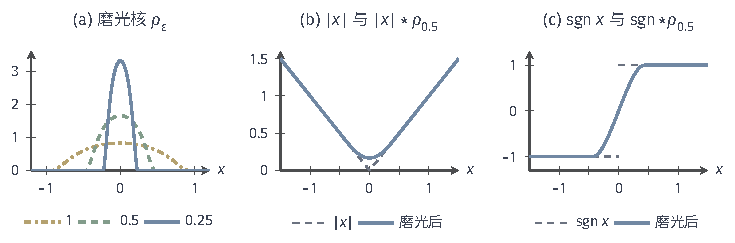
\includegraphics[width=124.4mm]{figures/02-abstract-mathematics/03-function-spaces/tikz/c4-mollifier/figure.pdf}
  \caption{一维磨光。(a)~磨光核$\rho_\varepsilon$，$\varepsilon=1,0.5,0.25$：支撑为$[-\varepsilon,\varepsilon]$，峰值约$0.829/\varepsilon$，面积均为$1$。(b)~$|x|$（虚线）与$|x|*\rho_{0.5}$（实线）：尖点被抹平，原点值约$0.167$，在$|x|\ge0.5$处两者重合。(c)~$\operatorname{sgn}x$与$\operatorname{sgn}*\rho_{0.5}$：后者光滑地从$-1$升到$1$，它恰好是(b)中光滑曲线的导数，体现$(|x|*\rho_\varepsilon)'=\operatorname{sgn}*\rho_\varepsilon$。}
  \label{fig:sob-mollifier}
\end{figure*}

\paragraph{$L^p$中的恢复}
要让磨光成为逼近，需要说明$u_\varepsilon\to u$。我们先考虑$\Omega=\mathbb R^d$且$u\in L^p(\mathbb R^d)$，$1\le p<\infty$；一般区域的情形随后用截断归结到这里。证明分三步。

第一步，磨光不放大$L^p$范数。$\rho_\varepsilon(x-\cdot)\,\mathrm dy$是质量为$1$的测度，对它使用Hölder不等式（$p>1$时把被积函数写成$|u|\rho_\varepsilon^{1/p}\cdot\rho_\varepsilon^{1/q}$），得
\[
 |u_\varepsilon(x)|^p\le\int|u(y)|^p\rho_\varepsilon(x-y)\,\mathrm dy .
\]
两边对$x$积分，非负被积函数可交换积分次序（定理~\ref{thm:analysis-tonelli-fubini}），而$\int\rho_\varepsilon(x-y)\,\mathrm dx=1$，于是
\begin{equation}
 \|u_\varepsilon\|_{L^p}\le\|u\|_{L^p} .
 \label{eq:sob-mollifier-contraction}
\end{equation}
同样的论证用于平均值之差，给出
\begin{equation}
 \|u_\varepsilon-u\|_{L^p}\le\sup_{|z|\le\varepsilon}\|u(\cdot-z)-u\|_{L^p} ,
 \label{eq:sob-mollifier-translation}
\end{equation}
因为$u_\varepsilon(x)-u(x)=\int[u(x-z)-u(x)]\rho_\varepsilon(z)\,\mathrm dz$也是关于质量为$1$的测度的平均。于是问题化为平移的连续性：小平移是否只引起小的$L^p$误差。

第二步，对紧支撑连续函数证明平移连续性。设$g$连续且支撑在紧集$K_0$内。由Heine--Cantor定理（定理~\ref{thm:metric-heine-cantor}），$g$一致连续，所以$\sup_x|g(x-z)-g(x)|\to0$（$z\to0$）。$|z|\le1$时差函数支撑在$\{x:\operatorname{dist}(x,K_0)\le1\}$内，这个集合的测度有限，记为$M$，于是$\|g(\cdot-z)-g\|_{L^p}\le M^{1/p}\sup_x|g(x-z)-g(x)|\to0$。

第三步，推广到一般$L^p$。由第~\ref{sec:fs-density-separability}节，紧支撑连续函数在$L^p(\mathbb R^d)$中稠密（$1\le p<\infty$）：先用简单函数逼近，再用连续截断逼近有限测度集合的示性函数。任给$\eta>0$，取这样的$g$使$\|u-g\|_{L^p}<\eta$。平移不改变$L^p$范数，所以
\[
 \begin{aligned}
 \|u(\cdot-z)-u\|_{L^p}&\le\|u(\cdot-z)-g(\cdot-z)\|_{L^p}+\|g(\cdot-z)-g\|_{L^p}+\|g-u\|_{L^p}\\
 &<2\eta+\|g(\cdot-z)-g\|_{L^p} .
 \end{aligned}
\]
令$z\to0$，右端的上极限不超过$2\eta$，而$\eta$任意，故平移连续性成立。代回式~\eqref{eq:sob-mollifier-translation}，得到$\|u_\varepsilon-u\|_{L^p}\to0$。

对一般开集$\Omega$和$u\in L^p(\Omega)$，取开集$V$，其闭包是$\Omega$内的紧集，记$\delta=\operatorname{dist}(V,\partial\Omega)$。把$u$在$\Omega$外补成零得到$\tilde u\in L^p(\mathbb R^d)$；当$\varepsilon<\delta$时，在$V$上$u_\varepsilon=\tilde u*\rho_\varepsilon$，所以$\|u_\varepsilon-u\|_{L^p(V)}\le\|\tilde u*\rho_\varepsilon-\tilde u\|_{L^p(\mathbb R^d)}\to0$。这就是磨光的局部$L^p$恢复。

$p=\infty$时结论不成立。在$(-1,1)$上，$H_\varepsilon=H*\rho_\varepsilon$连续，而$H$在原点两侧分别为$0$和$1$，所以在原点附近总有一侧满足$|H_\varepsilon-H|\ge1/2$，$\|H_\varepsilon-H\|_{L^\infty}$不趋于零。连续函数的一致极限仍连续，不连续的$L^\infty$函数不可能被连续函数一致逼近。

\paragraph{磨光与弱导数交换}
现在设$u$有弱导数$D^\alpha u\in L^1_{\mathrm{loc}}(\Omega)$。对$x\in\Omega_\varepsilon$，函数$y\mapsto\rho_\varepsilon(x-y)$是$\Omega$上的测试，其$y$导数满足$D_y^\alpha[\rho_\varepsilon(x-y)]=(-1)^{|\alpha|}(D^\alpha\rho_\varepsilon)(x-y)$。从式~\eqref{eq:sob-mollifier-derivative}出发，
\[
 D^\alpha u_\varepsilon(x)=(-1)^{|\alpha|}\int_\Omega u(y)\,D_y^\alpha[\rho_\varepsilon(x-y)]\,\mathrm dy
 =\int_\Omega D^\alpha u(y)\,\rho_\varepsilon(x-y)\,\mathrm dy ,
\]
第二个等号是弱导数的定义~\eqref{eq:sob-weak-derivative}用于这个测试。于是
\begin{equation}
 D^\alpha(u*\rho_\varepsilon)=(D^\alpha u)*\rho_\varepsilon\qquad\text{在 }\Omega_\varepsilon\text{ 上成立}.
 \label{eq:sob-mollifier-commute}
\end{equation}
左端是光滑函数的经典导数，右端是弱导数的磨光。图~\ref{fig:sob-mollifier}(b)(c)在$|x|$上验证了这一点：磨光后的$|x|$的经典导数，正是$\operatorname{sgn}x$的磨光。

把式~\eqref{eq:sob-mollifier-commute}与$L^p$恢复结合，就得到局部的光滑逼近。

\begin{theorem}[局部光滑逼近]
\label{thm:sob-local-approximation}
设$1\le p<\infty$，$u\in W^{k,p}(\Omega)$，$V$为开集且闭包是$\Omega$内的紧集。则$u_\varepsilon\in C^\infty(\Omega_\varepsilon)$，并且当$\varepsilon\to0$时$\|u_\varepsilon-u\|_{W^{k,p}(V)}\to0$。若$\Omega=\mathbb R^d$，则$\|u_\varepsilon-u\|_{W^{k,p}(\mathbb R^d)}\to0$。
\end{theorem}

\begin{proof}
光滑性已在前面证明。对每个$|\alpha|\le k$，由式~\eqref{eq:sob-mollifier-commute}，$D^\alpha u_\varepsilon-D^\alpha u=(D^\alpha u)_\varepsilon-D^\alpha u$在$V$上成立（$\varepsilon<\operatorname{dist}(V,\partial\Omega)$），而$D^\alpha u\in L^p(\Omega)$，由局部$L^p$恢复，它在$L^p(V)$中趋于零。有限多个分量都趋于零，Sobolev范数也趋于零。$\Omega=\mathbb R^d$时用全空间的恢复即可。
\end{proof}

这个定理是连接弱运算与经典计算的桥梁：凡是对光滑函数成立、又只涉及$W^{k,p}$范数连续量的等式或不等式，都可以先对$u_\varepsilon$证明，再令$\varepsilon\to0$。它对$W^{k,\infty}$不成立。例如任何$C^1$函数$v$在$(-1,1)$上都满足$\|v'-\operatorname{sgn}\|_{L^\infty}\ge1$：$v'$在原点连续，在原点附近的右侧与左侧分别接近同一个数$v'(0)$，而$\max(|v'(0)-1|,|v'(0)+1|)\ge1$。所以$|x|$不能在$W^{1,\infty}$范数下被$C^1$函数逼近。

\subsection{整域逼近与边界延拓}
\label{sec:sob-global-approximation}

定理~\ref{thm:sob-local-approximation}只在离边界有正距离的区域上逼近。靠近边界的地方，磨光半径必须越来越小，否则会读到区域外的值。解决办法是把函数切成许多块，每块离边界的距离不同，各自选择合适的磨光半径，再拼回去。切块需要一组光滑的权重。

\paragraph{局部有限的单位分解}
取递增的开集$G_j=\{x\in\Omega:|x|<j,\ \operatorname{dist}(x,\partial\Omega)>1/j\}$，$j\ge1$，并令$G_0=G_{-1}=\varnothing$。每个$G_j$的闭包是$\Omega$内的紧集，$\bigcup_jG_j=\Omega$。令
\[
 V_j=G_{j+1}\setminus\overline{G_{j-1}},\qquad j\ge1 .
\]
这些开集覆盖$\Omega$，并且是\term{局部有限}（locally finite）的：每个$x\in\Omega$属于某个$G_m$，而$G_m$只与$V_1,\ldots,V_{m+1}$相交，所以$x$的邻域$G_m$只与有限多个$V_j$相交。可以证明存在函数$\zeta_j\in C_c^\infty(V_j)$，满足$0\le\zeta_j\le1$，并且
\[
 \sum_{j\ge1}\zeta_j(x)=1\qquad(x\in\Omega).
\]
构造方法是：用引理~\ref{lem:sob-cutoff}在紧集$\overline{G_j}\setminus G_{j-1}$上取等于$1$、支撑在$V_j$内的截断$\eta_j$，则$\sum_i\eta_i$在每点是有限和且处处为正，令$\zeta_j=\eta_j/\sum_i\eta_i$。称$\{\zeta_j\}$为从属于覆盖$\{V_j\}$的\term{单位分解}（partition of unity）。

图~\ref{fig:sob-partition-unity}在$\Omega=(0,1)$上画出了一组这样的权重，那里用到边界距离的对数作分层，与上面的$G_j$略有不同，但性质相同：每个权重的支撑紧含于区域，越靠近边界的权重支撑越窄，每一点只有有限个（图中至多两个）权重非零，总和恒为$1$。

\begin{figure}[!htb]
  \centering
  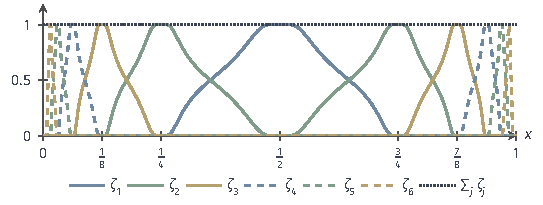
\includegraphics[width=92.0mm]{figures/02-abstract-mathematics/03-function-spaces/tikz/c4-partition-unity/figure.pdf}
  \caption{$\Omega=(0,1)$上的局部有限单位分解。记$s=\min(x,1-x)$为到边界的距离，$\zeta_j$支撑在$2^{-j-1}\le s\le2^{-j+1}$内，紧含于$(0,1)$；图中画出$\zeta_1,\ldots,\zeta_6$，每点至多两个权重非零，所有权重之和恒为$1$（点线）。越靠近边界，权重越密集，对应的磨光半径也要越小。}
  \label{fig:sob-partition-unity}
\end{figure}

\begin{theorem}[整域光滑逼近]
\label{thm:sob-meyers-serrin}
设$\Omega\subset\mathbb R^d$为任意开集，$k\ge0$，$1\le p<\infty$。则$C^\infty(\Omega)\cap W^{k,p}(\Omega)$在$W^{k,p}(\Omega)$中稠密。
\end{theorem}

\begin{proof}
固定$u\in W^{k,p}(\Omega)$与$\eta>0$。

第一步，分块。令$u_j=\zeta_ju$。由第~\ref{sec:sob-weak-derivative-def}节与光滑函数相乘的乘积法则（对高阶导数反复使用），$u_j\in W^{k,p}(\Omega)$，其各阶弱导数是$\zeta_j$的导数与$u$的弱导数的乘积之和，支撑在$V_j$内。由于$\zeta_j$紧支撑在$\Omega$内，把$u_j$在$\Omega$外补成零后属于$W^{k,p}(\mathbb R^d)$：对$\mathbb R^d$上的测试$\varphi$，用一个在$\operatorname{supp}\zeta_j$上为$1$、支撑在$\Omega$内的截断$\chi$，有$\int u_jD^\alpha\varphi=\int u_jD^\alpha(\chi\varphi)$，而$\chi\varphi$是$\Omega$上的测试。

第二步，逐块磨光并分配误差。对每个$j$，由定理~\ref{thm:sob-local-approximation}在$\mathbb R^d$上的结论，取$\varepsilon_j>0$足够小，使$v_j=u_j*\rho_{\varepsilon_j}$满足
\[
 \|v_j-u_j\|_{W^{k,p}(\mathbb R^d)}<\eta\,2^{-j},
\]
并且$\operatorname{supp}v_j\subset W_j:=G_{j+2}\setminus\overline{G_{j-2}}$。后一要求可以满足：$v_j$的支撑落在$\operatorname{supp}u_j$的$\varepsilon_j$邻域内，而$\overline{G_{j+1}}\subset G_{j+2}$、$\overline{G_{j-2}}\subset G_{j-1}$都是紧集含于开集，$V_j$与$W_j$的补集之间有正的间隔，取$\varepsilon_j$小于这个间隔即可。这里给第$j$块分配误差$\eta2^{-j}$，是为了让总和不超过$\eta$。

第三步，拼合。令$v=\sum_jv_j$。每点有邻域只与有限多个$W_j$相交，所以在这个邻域上$v$是有限个光滑函数之和，$v\in C^\infty(\Omega)$。同理$u=\sum_ju_j$在每个$G_m$上也只是有限和。于是在$G_m$上
\[
 \|v-u\|_{W^{k,p}(G_m)}\le\sum_j\|v_j-u_j\|_{W^{k,p}(\mathbb R^d)}<\sum_j\eta2^{-j}=\eta .
\]
令$m\to\infty$，由单调收敛定理（第~\ref{sec:measure-general-structure}节），$\|v-u\|_{W^{k,p}(\Omega)}\le\eta$。特别地$v\in W^{k,p}(\Omega)$。
\end{proof}

这个定理对任意开集成立，连边界的形状都不需要。但要读清它给出的是什么：逼近函数在$\Omega$\emph{内部}光滑，可能在边界附近剧烈振荡，并不是“光滑到边界”的函数，更不是紧支撑在$\Omega$内的测试函数。$C_c^\infty(\Omega)$在$W^{k,p}(\Omega)$中一般\emph{不}稠密。以$(0,1)$上的常数$1$为例：每个$\varphi\in C_c^\infty(0,1)$在端点附近为零，由式~\eqref{eq:sob-1d-sup-bound}（$p=2$，$L=1$），
\[
 1=|1-\varphi(0)|\le\|1-\varphi\|_{L^2}+\|(1-\varphi)'\|_{L^2}\le\sqrt2\,\|1-\varphi\|_{H^1},
\]
所以常数$1$到$C_c^\infty(0,1)$的$H^1$距离至少是$1/\sqrt2$。测试函数的闭包把“边界值为零”的信息保留了下来，这将在第~\ref{sec:sob-poincare}节定义$H_0^1$。

\paragraph{光滑到边界：从半空间反射开始}
许多论证需要更强的逼近：逼近函数在闭区域$\overline\Omega$上光滑，即是某个$C_c^\infty(\mathbb R^d)$函数在$\Omega$上的限制。思路是先把$u$延拓成全空间上的Sobolev函数，再在全空间磨光，最后限制回$\Omega$。延拓是关键，而延拓方式的好坏取决于边界。

最简单的区域是半空间$\mathbb R^d_+=\{x=(x',x_d):x_d>0\}$，这里$x'\in\mathbb R^{d-1}$。对光滑到边界的$u$，作偶反射
\[
 Eu(x',x_d)=u(x',|x_d|).
\]
它在$x_d=0$处连续，但沿$x_d$方向一般出现尖点。像$|x|$那样在两侧分别分部积分，边界面上的项因两侧的值相同而相消，所以$Eu$有弱导数：对$j<d$，$\partial_jEu(x',x_d)=(\partial_ju)(x',|x_d|)$；对$j=d$，$\partial_dEu(x',x_d)=\operatorname{sgn}(x_d)\,(\partial_du)(x',|x_d|)$。两侧对称，所以
\[
 \|Eu\|_{W^{1,p}(\mathbb R^d)}^p=2\,\|u\|_{W^{1,p}(\mathbb R^d_+)}^p .
\]
一般的$u\in W^{1,p}(\mathbb R^d_+)$可以先向区域内部平移一小段再磨光，得到光滑到边界的逼近，再由上式把延拓推广过去；这一细节属于补充，这里不展开。

与偶反射对照，零延拓（在$x_d<0$处令$u=0$）通常不行：若$u$在边界面上的值不为零，零延拓在边界面上产生跳跃，按阶跃函数的计算，它的$x_d$方向广义导数含有一个集中在边界面上的项，不是局部可积函数。图~\ref{fig:sob-reflection}在一维比较了两种延拓。只有当$u$的边界值为零时（确切含义见第~\ref{sec:sob-trace}节），零延拓才保持在$W^{1,p}$中。高阶空间中偶反射也不够，因为$x_d$方向的导数在反射后改变符号而跳跃；可以改用$Eu(x',x_d)=-3u(x',-x_d)+4u(x',-x_d/2)$（$x_d<0$），容易核对它在边界面上与$u$的值和一阶法向导数都相接。

\begin{figure}[!htb]
  \centering
  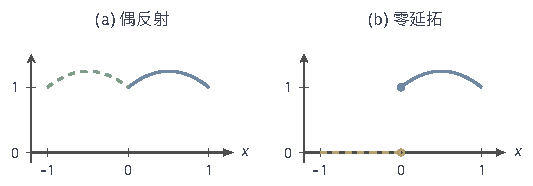
\includegraphics[width=90.2mm]{figures/02-abstract-mathematics/03-function-spaces/tikz/c4-reflection/figure.pdf}
  \caption{半区间上的两种延拓，$u(x)=1+x-x^2$（$0\le x\le1$），$u(0)=1$。(a)~偶反射$Eu(x)=u(|x|)$（虚线为延拓部分）：在原点连续而有尖点，弱导数$\operatorname{sgn}(x)u'(|x|)$局部可积，延拓保持在$W^{1,p}$中。(b)~零延拓：在原点跳跃$u(0)=1$，广义导数含$\delta_0$项，延拓不在$W^{1,p}$中。}
  \label{fig:sob-reflection}
\end{figure}

\paragraph{Lipschitz区域与延拓}
一般区域的边界可以弯曲，但只要它在局部可以拉直成半空间，就能沿用反射。

\begin{definition}[Lipschitz区域]
\label{def:sob-lipschitz-domain}
称有界开集$\Omega\subset\mathbb R^d$为\term{Lipschitz区域}（Lipschitz domain），若对每个$x_0\in\partial\Omega$，存在$r>0$、一个以$x_0$为原点的旋转后的坐标系$(x',x_d)$和Lipschitz函数$\gamma:\mathbb R^{d-1}\to\mathbb R$，使
\[
 \Omega\cap B(x_0,r)=\{x\in B(x_0,r):x_d>\gamma(x')\}.
\]
\end{definition}

也就是说，在每个边界点附近，区域位于一个Lipschitz函数图像的上方，边界就是这个图像。球、立方体、凸多面体都是Lipschitz区域：立方体的棱角处边界不光滑，但仍是局部的Lipschitz图像。挖去一条线段的圆盘（割缝圆盘）不是：割缝两侧都是区域，区域不能只位于割缝的一侧。尖角向内收缩得比任何Lipschitz图像都快的区域也不是。

\begin{theorem}[Lipschitz区域上的延拓]
\label{thm:sob-extension}
设$\Omega$为有界Lipschitz区域，$1\le p<\infty$。存在有界线性算子$E:W^{1,p}(\Omega)\to W^{1,p}(\mathbb R^d)$，使$Eu=u$在$\Omega$上几乎处处成立，并且所有$Eu$都支撑在同一个有界集合内。
\end{theorem}

证明思路如下，细节属于补充阅读。边界是紧集，可以用有限个满足定义的球$B(x_i,r_i)$覆盖，再加上一个紧含于$\Omega$的开集覆盖内部；取从属于这有限个开集的单位分解，把$u$分成有限块。内部那块直接零延拓，它在边界附近本来就是零。每个边界块用变换$(x',x_d)\mapsto(x',x_d-\gamma(x'))$拉直：这个变换和它的逆都是Lipschitz的，可以证明它们把$W^{1,p}$函数变成$W^{1,p}$函数，范数只差一个由$\gamma$的Lipschitz常数决定的倍数。拉直后在半空间上作偶反射，再变换回去。有限多块的延拓相加，得到$Eu$。这里每一步都需要边界是局部的Lipschitz图像，割缝圆盘之所以失败，正是因为割缝两侧都有区域，无法只向一侧反射。

\begin{theorem}[光滑到边界的逼近]
\label{thm:sob-smooth-up-to-boundary}
设$\Omega$为有界Lipschitz区域，$1\le p<\infty$。则$C_c^\infty(\mathbb R^d)$中函数在$\Omega$上的限制在$W^{1,p}(\Omega)$中稠密。
\end{theorem}

\begin{proof}
对$u\in W^{1,p}(\Omega)$，由定理~\ref{thm:sob-extension}得到紧支撑的$Eu\in W^{1,p}(\mathbb R^d)$。由定理~\ref{thm:sob-local-approximation}，$Eu*\rho_\varepsilon\to Eu$在$W^{1,p}(\mathbb R^d)$中成立，而$Eu*\rho_\varepsilon\in C_c^\infty(\mathbb R^d)$。限制到$\Omega$上，范数只会变小，所以$\|(Eu*\rho_\varepsilon)|_\Omega-u\|_{W^{1,p}(\Omega)}\le\|Eu*\rho_\varepsilon-Eu\|_{W^{1,p}(\mathbb R^d)}\to0$。
\end{proof}

记这类限制函数的全体为$C^\infty(\overline\Omega)$。与定理~\ref{thm:sob-meyers-serrin}比较，它多了边界正则性的条件，换来了在闭区域上光滑、各阶导数连续到边界的逼近函数。下一节的边界迹就要用到这一点：对光滑到边界的函数，边界值有经典含义，再用逼近推广到整个Sobolev空间。

% 第4章第5节：正则性、紧性与边界（嵌入与连续代表、紧嵌入、边界迹、零边界与Poincaré不等式）。

\section{正则性、紧性与边界}
\label{sec:sob-regularity}

Sobolev空间完备，光滑函数在其中稠密，但第~\ref{sec:sob-completeness}节末尾留下的问题还没有回答。本节分别研究四个问题：导数的积分控制能把函数值控制到什么程度；范数有界的函数列能否抽出强收敛子列；体积上的函数怎样拥有边界值；去掉常数方向以后，能否只用导数控制函数本身。四个问题都靠导数控制，但各自需要的条件不同，得到的结论也不能互相替代。

本节除特别说明外，都在有界Lipschitz区域$\Omega\subset\mathbb R^d$上讨论，并且只处理一阶空间$W^{1,p}(\Omega)$。区域有界保证小指数的$L^q$范数受大指数控制（$\|u\|_{L^q}\le|\Omega|^{1/q-1/p}\|u\|_{L^p}$，$q\le p$），边界为Lipschitz保证第~\ref{sec:sob-global-approximation}节的延拓与光滑到边界的逼近可用。

\subsection{积分指数与连续代表}
\label{sec:sob-embedding}

一维时，第~\ref{sec:sob-absolute-continuity}节证明了$W^{1,p}(a,b)$的元素都有连续代表，$p>1$时还是Hölder连续的。可是式~\eqref{eq:sob-power-membership}给出$|x|^{-1/4}\in W^{1,2}(B)$（$B$为$\mathbb R^3$中的单位球），它在原点无界。可见在高维，导数平方可积不足以保证连续。究竟是什么决定了结论？

\paragraph{缩放解释}
设想对全空间上的光滑紧支撑函数$u$有不等式$\|u\|_{L^q(\mathbb R^d)}\le C\|\nabla u\|_{L^p(\mathbb R^d)}$，常数$C$不依赖$u$。把$u$换成$u_\lambda(x)=u(\lambda x)$，$\lambda>0$。由换元$y=\lambda x$，
\[
 \|u_\lambda\|_{L^q}=\lambda^{-d/q}\|u\|_{L^q},\qquad\|\nabla u_\lambda\|_{L^p}=\lambda^{1-d/p}\|\nabla u\|_{L^p} .
\]
不等式对所有$\lambda$成立，两边的$\lambda$指数必须相等，否则令$\lambda\to0$或$\lambda\to\infty$就会破坏它。于是$-d/q=1-d/p$，即
\begin{equation}
 \frac1q=\frac1p-\frac1d,\qquad q=p^*:=\frac{dp}{d-p}\quad(1\le p<d).
 \label{eq:sob-sobolev-exponent}
\end{equation}
称$p^*$为$p$的\term{Sobolev共轭指数}（Sobolev conjugate exponent）。缩放论证只说明了指数必须是什么，并没有证明不等式成立；但它揭示了维数的作用：在$d$维中，把函数压缩到小尺度，导数的$L^p$范数按$\lambda^{1-d/p}$变化，$d$越大、$p$越小，导数就越“看不见”尖锐的集中。当$p>d$时，同样的计算用于Hölder商$|u(x)-u(y)|/|x-y|^\gamma$，它按$\lambda^\gamma$缩放，与$\lambda^{1-d/p}$匹配要求$\gamma=1-d/p$。

\begin{theorem}[Sobolev嵌入]
\label{thm:sob-embedding}
设$\Omega\subset\mathbb R^d$为有界Lipschitz区域。
\begin{enumerate}
 \item 若$1\le p<d$，则$W^{1,p}(\Omega)\subset L^{p^*}(\Omega)$，并存在常数$C$使$\|u\|_{L^{p^*}}\le C\|u\|_{W^{1,p}}$。由区域有界，对$1\le q\le p^*$也有$\|u\|_{L^q}\le C_q\|u\|_{W^{1,p}}$。
 \item 若$d<p<\infty$，则每个$u\in W^{1,p}(\Omega)$有一个在$\overline\Omega$上$\gamma=1-d/p$阶Hölder连续的代表$\tilde u$，并且
 \[
  \sup_{\overline\Omega}|\tilde u|+\sup_{x\neq y}\frac{|\tilde u(x)-\tilde u(y)|}{|x-y|^{\gamma}}\le C\|u\|_{W^{1,p}} .
 \]
\end{enumerate}
\end{theorem}

一个包含关系连同范数控制，称为\term{连续嵌入}（continuous embedding）：包含映射是有界线性算子。图~\ref{fig:sob-embedding-exponents}(a)在$(p,d)$平面上标出两种情形，(b)画出$p^*$随$p$的变化。$H^1=W^{1,2}$在$d=1$时落在Hölder一侧，得到$C^{0,1/2}$，与式~\eqref{eq:sob-1d-holder}一致；$d=3$时落在另一侧，$2^*=6$，得到$L^6$；$d=2$恰好在分界线上。

\begin{figure}[!htb]
  \centering
  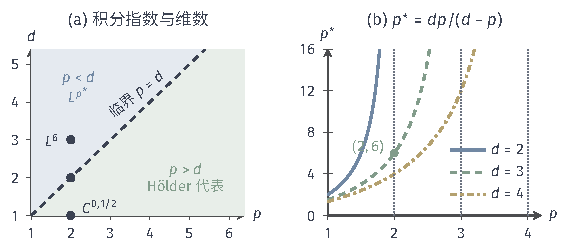
\includegraphics[width=96.3mm]{figures/02-abstract-mathematics/03-function-spaces/tikz/c4-embedding-exponents/figure.pdf}
  \caption{$W^{1,p}$的嵌入由积分指数与维数共同决定。(a)~$(p,d)$平面：$p<d$（蓝）时嵌入$L^{p^*}$，$p>d$（绿）时有Hölder连续代表，虚线$p=d$为临界情形；三个点是$p=2$、$d=1,2,3$，分别得到$C^{0,1/2}$、临界与$L^6$。(b)~$p^*=dp/(d-p)$随$p$增大而增大，$p\to d$时趋于无穷；$d=3$、$p=2$时$p^*=6$。}
  \label{fig:sob-embedding-exponents}
\end{figure}

\paragraph{幂函数检验指数的精确性}
回到$B\subset\mathbb R^d$上的$u=|x|^{-a}$。由式~\eqref{eq:sob-power-membership}，$u\in W^{1,p}(B)$当且仅当$(a+1)p<d$，即$a<d/p-1$；而$u\in L^q(B)$当且仅当$aq<d$。取$q=p^*$，条件$ap^*<d$化为$a<d/p^*=d/p-1$，与前者完全相同。所以每个在$W^{1,p}(B)$中的幂函数都在$L^{p^*}(B)$中，而对任何$q>p^*$，取$a$略小于$d/p-1$，便得到$W^{1,p}(B)$中不属于$L^q(B)$的函数：$p^*$不能再提高。$d=3$、$p=2$时，$a<1/2$的幂函数都在$L^6$中，且无界，这说明$p<d$时一般没有连续代表。

\paragraph{两种结论的机制}
两种情形的证明都从光滑函数出发，再借定理~\ref{thm:sob-smooth-up-to-boundary}推广。$p<d$的情形，先对$\mathbb R^d$上的光滑紧支撑函数证明$\|u\|_{L^{d/(d-1)}}\le\|\nabla u\|_{L^1}$：沿每个坐标方向，$|u(x)|\le\int_{\mathbb R}|\partial_ju|\,\mathrm dx_j$，把$d$个这样的估计相乘开$d-1$次根，再逐个坐标积分并反复使用Hölder不等式。一般的$p$由对$|u|^s$（适当的$s>1$）使用这一估计得到；有界Lipschitz区域上再用延拓算子转移到全空间。这一证明较长，属于补充阅读。

$p>d$的情形可以看出Hölder指数从哪里来。对光滑函数和以$x$为中心、半径$r$的球$B_r$，把$u(x)-u(y)$写成沿线段的导数积分，再对$y\in B_r$取平均，可以得到
\[
 \Bigl|u(x)-\frac{1}{|B_r|}\int_{B_r}u\,\mathrm dy\Bigr|\le C\int_{B_r}\frac{|\nabla u(y)|}{|x-y|^{d-1}}\,\mathrm dy .
\]
右端用Hölder不等式拆成$\|\nabla u\|_{L^p}$与$\bigl(\int_{B_r}|x-y|^{-(d-1)q}\mathrm dy\bigr)^{1/q}$，$q$为共轭指数。后一积分有限当且仅当$(d-1)q<d$，即$p>d$，此时它等于常数乘$r^{1-d/p}$。于是函数值与它在半径$r$的球上的平均之差不超过$Cr^{1-d/p}\|\nabla u\|_{L^p}$；两个相距$r$的点都和同一个球的平均比较，就得到$\gamma=1-d/p$阶的Hölder估计。$p\le d$时核$|x-y|^{1-d}$的$q$次幂不可积，这一步失效。两种结论的区别正在这里：$p<d$时得到的是更高的可积性，由体积上的积分累计；$p>d$时得到的是逐点的振荡控制，靠的是局部平均与中心值的比较。更高的可积性不等于连续，$L^{p^*}$中的函数仍可以无界。

\paragraph{临界情形$p=d$}
$d\ge2$、$p=d$时，两种结论都差一点。一方面，对每个有限的$q$，$W^{1,d}(\Omega)\subset L^q(\Omega)$：区域有界时$W^{1,d}(\Omega)\subset W^{1,s}(\Omega)$对每个$s<d$成立，而$s\to d$时$s^*=ds/(d-s)\to\infty$，所以任意有限$q$都被某个$s^*$超过。另一方面，$W^{1,d}$中的函数一般无界。在单位球$B\subset\mathbb R^d$中取
\[
 u(x)=\ln\ln\frac{e}{|x|} .
\]
记$r=|x|$，$s=\ln(e/r)\ge1$，则$|\nabla u|=1/(rs)$。按球坐标，$\int_B|\nabla u|^d\,\mathrm dx$与$\int_0^1\frac{r^{d-1}}{r^ds^d}\,\mathrm dr=\int_0^1\frac{\mathrm dr}{r\,(\ln(e/r))^d}$成正比，换元$s=\ln(e/r)$后化为$\int_1^\infty s^{-d}\,\mathrm ds$，$d\ge2$时有限；$u$本身只以$\ln\ln$的速度增长，属于$L^d(B)$。所以$u\in W^{1,d}(B)$，却在原点趋于无穷。

一维的$p=1=d$不受这一否定结论影响：第~\ref{sec:sob-absolute-continuity}节已经证明$W^{1,1}(a,b)$的元素有绝对连续代表，当然有界。原因是一维时单点的“容量”不为零：从$x$到$y$只有一条路径，函数的变化必须全部经过它，而在高维中，函数可以绕开一个点集中增长。

\paragraph{高阶空间}
同样的指数比较可以推广到$W^{k,p}$：每多一阶导数，在缩放中多出一个因子$\lambda$。若$kp<d$，则$W^{k,p}(\Omega)\subset L^q(\Omega)$，$1/q=1/p-k/d$；若$kp>d$，则函数有连续代表。特别地，$H^k(\Omega)$的元素在$k>d/2$时有连续代表，并且$\sup|\tilde u|\le C\|u\|_{H^k}$。这一结论使每个点值读取$u\mapsto\tilde u(x)$都是$H^k$上的有界线性泛函，第~\ref{chap:rkhs}章将以此为例说明哪些Hilbert函数空间具有连续的点值。分数阶空间与临界情形的完整分类这里不展开。

\subsection{有界函数列的紧性}
\label{sec:sob-compactness}

第~\ref{sec:sob-completeness}节的例子$u_n=\sin(n\pi x)/(n\pi)$在$H^1(0,1)$中有界，不在$H^1$中收敛，却在$L^2$中收敛。这不是巧合：导数的统一控制阻止了函数在小尺度上剧烈振荡，从而在较弱的范数下迫使序列聚集。

\begin{theorem}[紧嵌入]
\label{thm:sob-rellich}
设$\Omega\subset\mathbb R^d$为有界Lipschitz区域，$1\le p<\infty$。则$W^{1,p}(\Omega)$中的每个有界序列都有一个在$L^p(\Omega)$中收敛的子列。更一般地，$1\le p<d$时可以把$L^p$换成$L^q$，$1\le q<p^*$；$p\ge d$时可以换成任意有限$q$的$L^q$。
\end{theorem}

称这样的包含为\term{紧嵌入}（compact embedding）：包含映射把有界集映成相对紧集，按第~\ref{sec:ose-compact-def}节的说法，它是紧算子。下面给出$L^p$情形的证明，其中用到的延拓定理只给出了证明思路；$L^q$情形的推广由插值不等式得到，从略。

\begin{proof}
设$\|u_n\|_{W^{1,p}(\Omega)}\le M$。只需证明集合$\mathcal F=\{u_n\}$在$L^p(\Omega)$中全有界（第~\ref{sec:metric-totally-bounded}节）：$L^p$完备，完备空间中全有界集的闭包是紧的（定理~\ref{thm:metric-compact-complete-tb}），紧集中的序列有收敛子列。

第一步，转移到全空间。用定理~\ref{thm:sob-extension}的延拓算子，令$w_n=Eu_n$，则$\|w_n\|_{W^{1,p}(\mathbb R^d)}\le\|E\|M=:M'$，且所有$w_n$支撑在同一个有界集合内。只需证明$\{w_n\}$在$L^p(\mathbb R^d)$中全有界，限制到$\Omega$上不增大距离。

第二步，统一的平移估计。对光滑紧支撑函数$w$，$w(x+z)-w(x)=\int_0^1\nabla w(x+tz)\cdot z\,\mathrm dt$，两边取$L^p$范数并把范数移进对$t$的积分（Minkowski积分不等式），得
\[
 \|w(\cdot+z)-w\|_{L^p}\le|z|\,\|\nabla w\|_{L^p} .
\]
两边对$W^{1,p}$范数连续，由定理~\ref{thm:sob-local-approximation}的逼近，它对每个$w\in W^{1,p}(\mathbb R^d)$成立。结合式~\eqref{eq:sob-mollifier-translation}，
\[
 \|w_n*\rho_\varepsilon-w_n\|_{L^p}\le\varepsilon M'\qquad\text{对所有 }n\text{ 一致成立}.
\]
这一步是关键：导数的统一界把所有函数的磨光误差统一控制住了。

第三步，固定$\varepsilon$后的有限网。固定$\varepsilon$，函数$w_n*\rho_\varepsilon$都支撑在同一个紧集$K$内，并且由Hölder不等式，
\[
 |w_n*\rho_\varepsilon(x)|\le\|\rho_\varepsilon\|_{L^q}M',\qquad|\nabla(w_n*\rho_\varepsilon)(x)|\le\|\nabla\rho_\varepsilon\|_{L^q}M' ,
\]
$q$为共轭指数。所以这族函数在$K$上一致有界并有统一的Lipschitz常数。在$K$上取一个间距为$h$的有限网格，每个函数由它在网格点上的值确定到$\|\nabla\rho_\varepsilon\|_{L^q}M'\sqrt d\,h$以内；网格点上的值落在一个有界区间内，把这个区间分成有限多段，就把整族函数分成有限多组，每组内函数的一致距离任意小。一致距离乘$|K|^{1/p}$控制$L^p$距离，所以$\{w_n*\rho_\varepsilon\}$在$L^p$中全有界。这一论证正是第~\ref{sec:apx-arzela-ascoli}节Arzelà--Ascoli定理的机制。

第四步，合并。任给$\eta>0$，先取$\varepsilon$使$\varepsilon M'<\eta/3$，再取$\{w_n*\rho_\varepsilon\}$的有限$\eta/3$网$\{g_1,\ldots,g_N\}$。对每个$n$，选$g_i$与$w_n*\rho_\varepsilon$相距小于$\eta/3$，则$\|w_n-g_i\|_{L^p}<\varepsilon M'+\eta/3<\eta$。所以$\{w_n\}$有有限$\eta$网，全有界。
\end{proof}

证明清楚地显示了三种条件各自的职责。导数的统一界给出统一的平移估计，使磨光误差与$n$无关；区域有界（经延拓后支撑在同一有界集内）使固定尺度的函数族只需有限个网格点描述；目标范数$L^p$比$W^{1,p}$弱，才允许用磨光后的函数近似原函数。

\paragraph{与弱收敛子列的对照}
$1<p<\infty$时，$W^{1,p}(\Omega)$是自反空间，由第~\ref{sec:lfo-weak-subsequence}节，有界序列有弱收敛子列$u_{n_k}\rightharpoonup u$。紧嵌入把这一结论加强了：同一子列在$L^p$中\emph{强}收敛到$u$。原因是紧算子把弱收敛序列映成强收敛序列。在优化与变分问题中，这一组合经常这样使用：从极小化序列的有界性抽出弱收敛子列，再借紧嵌入让低阶项强收敛。但紧嵌入本身只是关于函数列的结论，并不是某个具体方程的可解性定理；把它用于具体问题时，还需要说明目标函数或方程项怎样在这种收敛下保持。

\paragraph{临界指数处的失紧}
定理~\ref{thm:sob-rellich}中$q<p^*$是严格不等式。在临界指数$q=p^*$处，嵌入仍连续，但不再是紧的。取$\varphi\in C_c^\infty(B)$非零，$B$为单位球，$1\le p<d$，令
\[
 u_\lambda(x)=\lambda^{(d-p)/p}\varphi(\lambda x),\qquad\lambda\ge1 .
\]
$u_\lambda$支撑在半径$1/\lambda$的球内。由缩放公式，$\|\nabla u_\lambda\|_{L^p}=\|\nabla\varphi\|_{L^p}$与$\|u_\lambda\|_{L^{p^*}}=\|\varphi\|_{L^{p^*}}$都不随$\lambda$改变，而$\|u_\lambda\|_{L^p}=\lambda^{-1}\|\varphi\|_{L^p}\to0$。所以$(u_\lambda)$在$W^{1,p}(B)$中有界。若某个子列在$L^{p^*}(B)$中收敛，由于它在$L^p$中收敛到$0$，$L^{p^*}$极限也只能是$0$（$L^{p^*}$收敛推出$L^p$收敛），与$\|u_\lambda\|_{L^{p^*}}$恒为常数矛盾。函数的质量向一点集中，在$L^{p^*}$中“看起来”一直一样大，却不收敛到任何东西。图~\ref{fig:sob-compactness-loss}(a)画出$d=3$、$p=2$时的径向剖面$u_\lambda(r)=\lambda^{1/2}\psi(\lambda r)$。

\begin{figure}[!htb]
  \centering
  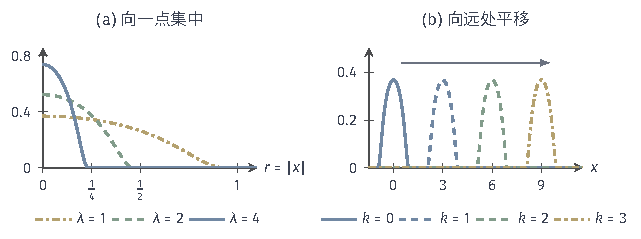
\includegraphics[width=108.6mm]{figures/02-abstract-mathematics/03-function-spaces/tikz/c4-compactness-loss/figure.pdf}
  \caption{两种失去紧性的方式。(a)~临界集中：$d=3$、$p=2$，$u_\lambda(x)=\lambda^{1/2}\psi(\lambda|x|)$的径向剖面，$\lambda=1,2,4$；峰值按$\lambda^{1/2}$升高，支撑半径按$1/\lambda$缩小，$\|\nabla u_\lambda\|_{L^2}$与$\|u_\lambda\|_{L^6}$不变，$\|u_\lambda\|_{L^2}\to0$。(b)~无界区域上的平移：$\psi(x-3k)$，$k=0,1,2,3$，形状和范数都不变，支撑互不相交，向远处逃逸。}
  \label{fig:sob-compactness-loss}
\end{figure}

\paragraph{无界区域上的逃逸}
区域有界的条件也不能去掉。在$\mathbb R^d$上取非零$\varphi\in C_c^\infty(\mathbb R^d)$与单位向量$e$，令$u_n(x)=\varphi(x-3n\,r_0e)$，其中$r_0$使$\operatorname{supp}\varphi\subset B(0,r_0)$。每个$u_n$的$W^{1,p}$范数都等于$\varphi$的范数，支撑两两不交，所以$\|u_n-u_m\|_{L^p}=2^{1/p}\|\varphi\|_{L^p}$（$n\neq m$），任何子列都不是$L^p$中的Cauchy列。函数没有集中，而是整体跑到了无穷远（图~\ref{fig:sob-compactness-loss}(b)，一维时取$\varphi=\psi$、$r_0=1$）。有界区域上，延拓后支撑被限制在同一有界集内，这种逃逸不会发生。

\subsection{边界迹}
\label{sec:sob-trace}

许多问题要给函数指定边界值。可是$W^{1,p}(\Omega)$的元素是几乎处处等价类，而$\partial\Omega$在$\mathbb R^d$中是Lebesgue零测集，任意修改一个代表在边界上的值，得到的仍是同一个元素。“$u$在边界上的值”因此需要重新定义，而不能取一个代表直接限制。

\paragraph{一维端点估计}
一维的答案已经有了。$u\in H^1(a,b)$有唯一的连续代表，式~\eqref{eq:sob-1d-sup-bound}在端点给出
\[
 |\tilde u(a)|\le L^{-1/2}\|u\|_{L^2}+L^{1/2}\|u'\|_{L^2}\le C\|u\|_{H^1(a,b)} .
\]
端点值由$H^1$范数控制，这正是高维要推广的东西。只有$L^2$控制是不够的：$u_n(x)=\max(1-nx,0)$在$(0,1)$上满足$u_n(0)=1$，而$\|u_n\|_{L^2}^2=\int_0^{1/n}(1-nx)^2\,\mathrm dx=1/(3n)\to0$，端点值不受$L^2$范数控制。

\paragraph{半空间上的迹估计}
高维的关键估计可以在半空间上完整证明。设$u\in C_c^\infty(\mathbb R^d)$，限制在$\overline{\mathbb R^d_+}$上考虑。固定$x'\in\mathbb R^{d-1}$，沿$x_d$方向从边界点$(x',0)$向内积分（图~\ref{fig:sob-trace}(b)）：$|u(x',t)|^2$在$t$大时为零，所以
\[
 \begin{aligned}
 |u(x',0)|^2&=-\int_0^\infty\partial_t\bigl(|u(x',t)|^2\bigr)\,\mathrm dt\\
 &\le2\int_0^\infty|u|\,|\partial_du|\,\mathrm dt\le\int_0^\infty\bigl(|u|^2+|\partial_du|^2\bigr)\,\mathrm dt ,
 \end{aligned}
\]
最后一步用了$2ab\le a^2+b^2$。再对$x'\in\mathbb R^{d-1}$积分，得到
\begin{equation}
 \int_{\mathbb R^{d-1}}|u(x',0)|^2\,\mathrm dx'\le\|u\|_{L^2(\mathbb R^d_+)}^2+\|\partial_du\|_{L^2(\mathbb R^d_+)}^2\le\|u\|_{H^1(\mathbb R^d_+)}^2 .
 \label{eq:sob-half-space-trace}
\end{equation}
边界值的$L^2$大小被体积上函数和法向导数的$L^2$大小控制。这与一维端点估计是同一个机制：沿着垂直于边界的每一条线，都是一个一维问题。

\begin{figure}[!htb]
  \centering
  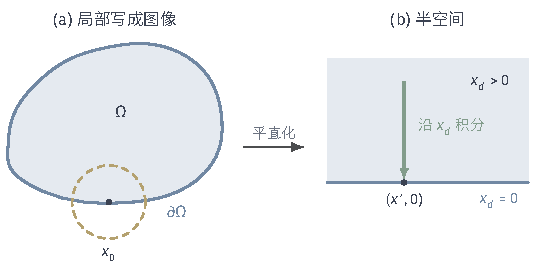
\includegraphics[width=90.3mm]{figures/02-abstract-mathematics/03-function-spaces/tikz/c4-trace/figure.pdf}
  \caption{边界迹的局部化与平直化。(a)~有界Lipschitz区域$\Omega$：边界点$x_0$附近的球（虚线）内，边界是Lipschitz函数的图像，区域位于图像一侧。(b)~拉直后成为半空间$\{x_d>0\}$：从边界点$(x',0)$沿$x_d$方向向内积分，边界值的平方被这条线上$|u|^2+|\partial_du|^2$的积分控制，再对$x'$积分即得式~\eqref{eq:sob-half-space-trace}。}
  \label{fig:sob-trace}
\end{figure}

\paragraph{Lipschitz区域上的迹定理}
在一般的有界Lipschitz区域上，边界需要配上\term{表面测度}（surface measure）$\mathrm dS$。在定义~\ref{def:sob-lipschitz-domain}的一个局部图像$x_d=\gamma(x')$上，约定$\mathrm dS=\sqrt{1+|\nabla\gamma(x')|^2}\,\mathrm dx'$；Lipschitz函数几乎处处可微且梯度有界，所以这个因子在$1$与$\sqrt{1+\mathrm{Lip}(\gamma)^2}$之间，边界上的$L^2$范数与拉直后$\mathbb R^{d-1}$上的$L^2$范数相差有界倍数。不同局部图像重叠处给出相同的测度，这里不加证明地使用这一点。记$L^2(\partial\Omega)=L^2(\partial\Omega,\mathrm dS)$。

\begin{theorem}[迹定理]
\label{thm:sob-trace}
设$\Omega$为有界Lipschitz区域。存在常数$C$，使所有$u\in C^\infty(\overline\Omega)$满足
\begin{equation}
 \|u|_{\partial\Omega}\|_{L^2(\partial\Omega)}\le C\|u\|_{H^1(\Omega)} ,
 \label{eq:sob-trace-inequality}
\end{equation}
并且存在唯一的有界线性算子$\operatorname{Tr}:H^1(\Omega)\to L^2(\partial\Omega)$，对$u\in C^\infty(\overline\Omega)$有$\operatorname{Tr}u=u|_{\partial\Omega}$。
\end{theorem}

式~\eqref{eq:sob-trace-inequality}的证明思路是：用有限个边界球和一个内部开集覆盖$\overline\Omega$，取从属的单位分解，把$u$分成有限块；内部那块在边界上为零；每个边界块用$(x',x_d)\mapsto(x',x_d-\gamma(x'))$拉直，变成半空间上的光滑紧支撑函数，套用式~\eqref{eq:sob-half-space-trace}，再把拉直变换和表面测度因子带来的有界倍数计入常数。这一路线把一维的端点估计逐线推广到一般区域，细节属于补充阅读。

算子$\operatorname{Tr}$的构造则完全可以在这里完成。对$u\in H^1(\Omega)$，由定理~\ref{thm:sob-smooth-up-to-boundary}取$u_n\in C^\infty(\overline\Omega)$在$H^1$中收敛到$u$。由式~\eqref{eq:sob-trace-inequality}，
\[
 \|u_n|_{\partial\Omega}-u_m|_{\partial\Omega}\|_{L^2(\partial\Omega)}\le C\|u_n-u_m\|_{H^1(\Omega)},
\]
所以边界限制构成$L^2(\partial\Omega)$中的Cauchy列，由$L^2$的完备性收敛到某个$g$。极限不依赖逼近列的选取：若$v_n\to u$是另一列，交错排列的$(u_1,v_1,u_2,v_2,\ldots)$仍在$H^1$中收敛到$u$，其边界限制也收敛，于是两个子列的极限相同。令$\operatorname{Tr}u=g$。线性由极限的线性得到，范数界$\|\operatorname{Tr}u\|_{L^2(\partial\Omega)}\le C\|u\|_{H^1(\Omega)}$由式~\eqref{eq:sob-trace-inequality}取极限得到。唯一性来自$C^\infty(\overline\Omega)$的稠密性：两个有界线性算子在稠密子集上一致，便处处一致。

称$\operatorname{Tr}u$为$u$的\term{边界迹}（trace）。它的输出是$L^2(\partial\Omega)$中的等价类，不是某一个边界点上的数：在$d\ge2$时，$H^1$函数可以在边界点附近无界（把前面的幂函数例子中心放到边界点上），单点的值没有意义，只有沿边界的$L^2$平均有意义。迹的像也不是整个$L^2(\partial\Omega)$：可以证明它是一个由边界上“半阶导数”刻画的更小的空间，精确描述需要分数阶Sobolev空间，本章不展开。

\subsection{零边界、零均值与导数控制}
\label{sec:sob-poincare}

有了迹，就可以说一个$H^1$函数“在边界上为零”。本小节用它定义零边界空间，并回答第~\ref{sec:sob-norms}节留下的问题：排除常数方向以后，导数能否单独控制函数。

\paragraph{零边界空间}
第~\ref{sec:sob-global-approximation}节看到，$C_c^\infty(\Omega)$的$H^1$闭包比$H^1(\Omega)$小，它保留了“在边界附近为零”的信息。我们把这个闭包取作定义。

\begin{definition}[零边界Sobolev空间]
\label{def:sob-h01}
设$\Omega\subset\mathbb R^d$为开集。称$C_c^\infty(\Omega)$在$H^1(\Omega)$范数下的闭包为$H_0^1(\Omega)$。
\end{definition}

这个定义不涉及任何代表的边界值，对任意开集都有意义；作为$H^1(\Omega)$的闭子空间，它本身是Hilbert空间。在有界Lipschitz区域上，它可以用迹刻画。$C_c^\infty(\Omega)$中的函数在边界附近为零，迹为零；$\operatorname{Tr}$连续，零迹在$H^1$极限下保持，所以$H_0^1(\Omega)\subset\ker\operatorname{Tr}$。反向包含也成立：

\begin{theorem}[零迹刻画]
\label{thm:sob-h01-kernel}
设$\Omega$为有界Lipschitz区域，则$H_0^1(\Omega)=\ker\operatorname{Tr}=\{u\in H^1(\Omega):\operatorname{Tr}u=0\}$。
\end{theorem}

反向包含的证明思路是：对零迹的$u$，在每个局部图像中把$u$沿远离边界的方向推进一小段，再乘以在边界附近为零的截断并磨光；零迹保证截断引起的误差随推进距离趋于零。细节属于补充阅读。一维时这一刻画很直观：$H_0^1(a,b)$恰好由连续代表满足$\tilde u(a)=\tilde u(b)=0$的$H^1$函数组成。

\paragraph{固定边界值的函数集合}
设边界数据$g$是某个$G\in H^1(\Omega)$的迹，$g=\operatorname{Tr}G$。所有迹等于$g$的$H^1$函数组成集合
\[
 \{v\in H^1(\Omega):\operatorname{Tr}v=g\}=G+H_0^1(\Omega).
\]
等式成立是因为$\operatorname{Tr}v=\operatorname{Tr}G$等价于$\operatorname{Tr}(v-G)=0$，再用定理~\ref{thm:sob-h01-kernel}。这个集合是闭仿射子空间，它的“方向”是$H_0^1(\Omega)$：在保持边界值的前提下，允许的扰动恰好是零迹函数。这一结构是边值问题弱形式的出发点，但具体方程、变分条件和法向导数的含义需要额外的正则性和目标函数，属于优化与微分方程的话题，这里只建立允许函数的集合。

\paragraph{去除常数方向}
现在回到导数半范数$\|\nabla u\|_{L^2}$。常数的梯度为零，所以在整个$H^1(\Omega)$上，$\|\nabla u\|_{L^2}$不可能控制$\|u\|_{L^2}$。图~\ref{fig:sob-poincare}(a)就是这个反例。要让导数单独控制函数，必须用某种条件排除常数。零边界和零均值是两种典型的方式。

\begin{figure*}[!htb]
  \centering
  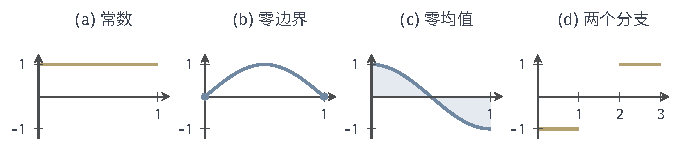
\includegraphics[width=114.4mm]{figures/02-abstract-mathematics/03-function-spaces/tikz/c4-poincare/figure.pdf}
  \caption{Poincaré不等式中约束的作用。(a)~常数$u=1$：$u'=0$而$\|u\|_{L^2}=1$，没有约束时导数控制不了函数。(b)~零边界$u=\sin(\pi x)$：$\|u\|_{L^2}/\|u'\|_{L^2}=1/\pi$。(c)~零均值$u=\cos(\pi x)$（阴影正负面积相等）：比值同为$1/\pi$。(d)~两个分支$(0,1)\cup(2,3)$上分别取$-1$与$1$：均值为零、导数为零，说明零均值形式需要区域连通。}
  \label{fig:sob-poincare}
\end{figure*}

\begin{theorem}[Poincaré不等式]
\label{thm:sob-poincare}
\begin{enumerate}
 \item 设$\Omega$为有界开集。存在常数$C$，使所有$u\in H_0^1(\Omega)$满足$\|u\|_{L^2}\le C\|\nabla u\|_{L^2}$。
 \item 设$\Omega$为有界连通Lipschitz区域，$u_\Omega=|\Omega|^{-1}\int_\Omega u\,\mathrm dx$为均值。存在常数$C$，使所有$u\in H^1(\Omega)$满足$\|u-u_\Omega\|_{L^2}\le C\|\nabla u\|_{L^2}$。
\end{enumerate}
\end{theorem}

\paragraph{区间上的直接证明}
先在区间$(a,b)$上用积分表示直接证明，$L=b-a$。对零边界情形，由$H_0^1$的定义和稠密性，只需对$u\in C_c^\infty(a,b)$证明（两边对$H^1$范数连续）。此时$u(a)=0$，$u(x)=\int_a^xu'(t)\,\mathrm dt$，由Cauchy--Schwarz不等式$|u(x)|^2\le(x-a)\|u'\|_{L^2}^2$，对$x$积分得
\[
 \|u\|_{L^2}^2\le\frac{L^2}{2}\|u'\|_{L^2}^2,\qquad\|u\|_{L^2}\le\frac{L}{\sqrt2}\|u'\|_{L^2} .
\]
对零均值情形，用连续代表，$|\tilde u(x)-\tilde u(y)|\le L^{1/2}\|u'\|_{L^2}$（式~\eqref{eq:sob-1d-holder}，$p=2$）。由于$\tilde u(x)-u_\Omega=L^{-1}\int_a^b(\tilde u(x)-\tilde u(y))\,\mathrm dy$，有$|\tilde u(x)-u_\Omega|\le L^{1/2}\|u'\|_{L^2}$，平方后对$x$积分得$\|u-u_\Omega\|_{L^2}\le L\|u'\|_{L^2}$。这两个常数都不是最优的。在$(0,1)$上，$\sin(\pi x)$与$\cos(\pi x)$分别满足零边界与零均值，比值$\|u\|_{L^2}/\|u'\|_{L^2}$都等于$1/\pi\approx0.318$（图~\ref{fig:sob-poincare}(b)(c)）；可以证明$L/\pi$就是两种情形的最优常数，而上面的直接估计给出$L/\sqrt2\approx0.707L$与$L$。

\paragraph{一般区域的反证路线}
高维没有这样简单的积分表示，但紧嵌入提供了一条反证路线。以零均值情形为例。反设不等式不成立，则对每个$n$有$u_n\in H^1(\Omega)$，$u_n$的均值为零，$\|u_n\|_{L^2}=1$，而$\|\nabla u_n\|_{L^2}<1/n$。

第一步，序列在$H^1$中有界（$\|u_n\|_{H^1}^2<1+1/n^2$），由定理~\ref{thm:sob-rellich}，有子列（仍记作$u_n$）在$L^2$中收敛到某个$u$。$L^2$收敛保持范数与均值，所以$\|u\|_{L^2}=1$，$u$的均值为零。

第二步，极限在$H^1$中取得，且梯度为零。由于$\|u_n-u_m\|_{H^1}^2=\|u_n-u_m\|_{L^2}^2+\|\nabla u_n-\nabla u_m\|_{L^2}^2$，前一项因$L^2$收敛而趋零，后一项不超过$(1/n+1/m)^2$，所以$(u_n)$是$H^1$中的Cauchy列。由定理~\ref{thm:sob-complete}，它在$H^1$中收敛，极限只能是$u$，并且$\|\nabla u\|_{L^2}=\lim\|\nabla u_n\|_{L^2}=0$。

第三步，梯度为零的函数在连通区域上是常数。由式~\eqref{eq:sob-mollifier-commute}，$\nabla(u*\rho_\varepsilon)=(\nabla u)*\rho_\varepsilon=0$在$\Omega_\varepsilon$上成立。对闭包含于$\Omega$的任一球$B$，$\varepsilon$足够小时$B\subset\Omega_\varepsilon$，光滑函数$u*\rho_\varepsilon$在连通的$B$上为常数；令$\varepsilon\to0$，由局部$L^2$恢复，$u$在$B$上几乎处处等于这些常数的极限。相交的两个球上常数相同，而连通开集中任意两点可以用有限个依次相交的球连接，所以$u$在$\Omega$上几乎处处为同一个常数。均值为零迫使这个常数为零，与$\|u\|_{L^2}=1$矛盾。

零边界情形的反证几乎相同。先说明可以只在球上讨论：取一个闭包包含$\overline\Omega$的开球$B_0$，把$H_0^1(\Omega)$的函数在$\Omega$外补成零。对$C_c^\infty(\Omega)$中的函数，零延拓属于$C_c^\infty(B_0)$，$H^1$范数不变；由闭包的定义，零延拓把$H_0^1(\Omega)$等距地映入$H_0^1(B_0)$，并且像中的函数在$B_0\setminus\Omega$上为零。于是只需对球$B_0$上、在$B_0\setminus\Omega$上为零的$H_0^1$函数证明不等式。$B_0$是连通的Lipschitz区域，第一步的紧嵌入可用；第二步的极限$u$仍属于闭子空间$H_0^1(B_0)$，在$B_0\setminus\Omega$上为零，梯度为零；第三步给出$u$在$B_0$上为常数，而$B_0\setminus\Omega$包含一个正测度的环形区域，所以常数为零，同样矛盾。这一论证不需要$\Omega$连通或有Lipschitz边界。

\paragraph{条件为什么不能少}
反证路线清楚地显示了每个条件的作用：紧嵌入把“导数趋于零”变成一个强收敛的极限；弱梯度为零只能推出“在每个连通分支上为常数”；最后由零边界或零均值把常数消去。去掉连通性，零均值不足以消去常数，图~\ref{fig:sob-poincare}(d)在$(0,1)\cup(2,3)$上取$-1$与$1$，均值为零、导数为零，不等式失败。去掉约束，常数函数本身就是反例。去掉区域有界，紧嵌入失效：在整条实轴上，$u_R(x)=\psi(x/R)$满足$\|u_R\|_{L^2}=R^{1/2}\|\psi\|_{L^2}$而$\|u_R'\|_{L^2}=R^{-1/2}\|\psi'\|_{L^2}$，比值随$R$无界，零边界也救不回来。

% 第4章第6节：本章小结。

\section{本章小结}
\label{sec:sob-summary}

本章开头的问题是：经典导数失效以后，怎样保存变化的信息，以及控制了函数和它的变化之后能得到什么。回答由一条对象链和四个分支问题组成，图~\ref{fig:sob-object-relations}把它们画在一起。

\begin{figure*}[!htb]
  \centering
  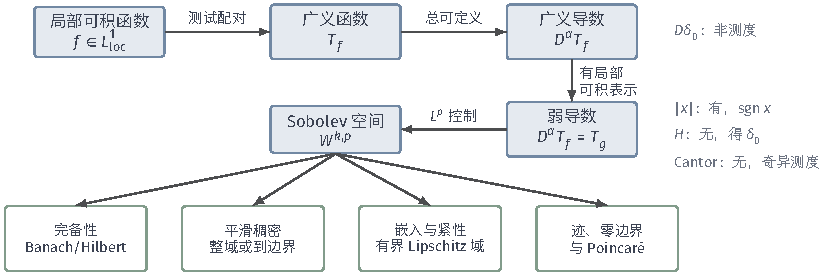
\includegraphics[width=140.6mm]{figures/02-abstract-mathematics/03-function-spaces/tikz/c4-object-relations/figure.pdf}
  \caption{本章的对象关系。上行：局部可积函数经测试配对成为广义函数，广义导数总能定义；只有当广义导数有局部可积表示时才得到弱导数，再加上$L^p$大小的控制便得到Sobolev空间。下行：Sobolev空间上分别研究的四个问题，其中嵌入、紧性与迹需要有界Lipschitz区域等条件。右侧的例子检验对象链的边界：$\delta_0$的导数不是测度，$|x|$有弱导数，阶跃与Cantor函数的广义导数分别是点质量与奇异测度。}
  \label{fig:sob-object-relations}
\end{figure*}

\paragraph{对象链及其边界}
从分部积分出发，我们把导数转移到紧支撑的光滑测试上。局部可积函数通过积分配对成为广义函数，广义导数对每个广义函数都有定义，但输出可能超出函数甚至测度的范围，$D\delta_0$就是这样。当广义导数恰好由一个局部可积函数表示时，称之为弱导数；测试函数能区分局部可积函数，所以弱导数在几乎处处意义下唯一。尖点函数$|x|$有弱导数$\operatorname{sgn}x$；阶跃函数的广义导数是$\delta_0$，Cantor函数的广义导数是集中在零测集上的奇异测度，两者都没有弱导数，尽管它们几乎处处有经典导数。在一维，弱可微恰好等价于有绝对连续代表，即能从导数积分恢复函数；导数的积分指数$p$进一步决定代表的Hölder指数$1-1/p$。把函数和直到$k$阶的弱导数的$L^p$大小同时放进范数，得到Sobolev空间$W^{k,p}$；零阶项控制水平，导数项控制变化。

\paragraph{四个问题各自的条件}
在Sobolev空间上，我们分别回答了几个不能互相代替的问题。完备性对任意开集成立，$H^k$因而是Hilbert空间，但它不提供连续代表、边界值或强收敛子列。光滑逼近分三层：磨光与弱导数交换给出局部逼近；单位分解把它拼成任意开集上的内部光滑逼近；光滑到边界的逼近需要Lipschitz边界和延拓。连续嵌入由积分指数与维数比较决定：$p<d$时得到$L^{p^*}$，$p>d$时得到Hölder连续代表，临界的$p=d\ge2$两者都差一点；缩放论证解释了$p^*=dp/(d-p)$的来源，幂函数检验了它的精确性。紧嵌入在有界Lipschitz区域上把有界序列变成$L^q$（$q<p^*$）中收敛的子列，在临界指数处因集中而失效，在无界区域上因平移逃逸而失效。边界迹把光滑函数的边界限制延拓为$H^1(\Omega)\to L^2(\partial\Omega)$的有界算子，输出是边界上的等价类；零迹函数恰好构成$H_0^1$。Poincaré不等式在排除常数方向之后，让导数单独控制函数，零边界与零均值是两种排除方式，后者还需要区域连通。

\paragraph{与后续内容的关系}
这些空间和工具为后面的问题提供了语言。第~\ref{chap:rkhs}章研究点值读取连续的Hilbert函数空间，本章一维的端点估计和$H^k$（$k>d/2$）的连续代表是那里的具体例子，而高维$H^1$在一点附近可以无界，则说明点值连续并非理所当然。在优化中，Sobolev空间用来指定目标函数的定义域，$G+H_0^1$给出保持边界值的可行扰动，紧嵌入配合弱收敛子列处理极小化序列；在微分方程与演化问题中，它们用来表达弱解。本章只建立空间、微分和边界的工具，不由这些工具直接断言某个具体问题有解。


\chapter{再生核Hilbert空间}
\label{chap:rkhs}

设想我们在区间上布置了几个传感器，只能读出未知函数在这些位置的取值。要把这些读数当作关于函数的可靠信息，至少需要两件事：函数本身改动一点时，读数只改动一点；读数背后对应的函数方向要能具体写出来。第~\ref{chap:linear-functionals-operators}章已经看到，在$L^2$这样的积分空间里，单点取值往往连定义都没有；即便限制为连续函数，平方积分很小的函数也可能在某一点取值很大。另一方面，第~\ref{chap:weak-derivatives-sobolev}章中一维Sobolev函数有连续代表，点值受Sobolev范数控制。本章研究的正是这一类空间：由真实函数组成、点值读取连续的Hilbert空间。

本章要回答四个相互衔接的问题。第一，点值连续时，每个点的读取能否写成与某个固定函数的内积，这些函数合在一起记录了什么？第~\ref{sec:rkhs-point-evaluation}节用Riesz表示得到再生核，并说明核怎样同时刻画单点读取的强弱与读数随位置变化的方式。第二，能否反过来只给定一个二元函数就确定空间？第~\ref{sec:rkhs-construction}节从半正定核出发构造空间，再给出特征映射与核运算两种可检查的构造途径。第三，只拿到有限个点值时，函数的哪些部分被看见、哪些部分完全看不见？第~\ref{sec:rkhs-finite-observations}节用正交投影回答这个问题，并把有限维计算写成核矩阵。第四，若在输入集上再给定一个测度，核积分算子的谱能否提供另一种正交表示？第~\ref{sec:rkhs-spectral}节建立Mercer展开，比较两种范数的谱权重，并对比按谱截断与按观测中心投影得到的两种有限表示。

前两节只用到集合、Hilbert空间与有界线性泛函，不需要测度；测度只在最后一节出现，用来产生积分算子与新的正交坐标。全章约定函数取实值，输入集$X$是非空集合，没有额外说明时不要求它带距离或测度。三个例子贯穿全章：仿射核$K(x,z)=1+xz$给出二维空间，便于逐个坐标核对；$[0,1]$上的最小值核$K(x,z)=\min(x,z)$给出与一维Sobolev空间相连的无限维空间；高斯核则代表光滑且严格正定的核。如何用核截面逼近一般连续函数、如何用有限个代表覆盖整类函数，留到第~\ref{chap:function-approximation}章讨论。

% 第5章第1节：点值与再生核（点值泛函与再生关系、再生核的性质）。

\section{点值与再生核}
\label{sec:rkhs-point-evaluation}

本节固定一个由真实函数组成的Hilbert空间，要求每个点的取值都连续地依赖于函数。第~\ref{sec:lfo-point-evaluation}节已经把点值读取的良定义与有界性分开讨论；这里把两项要求同时作为空间的前提，再用第~\ref{sec:lfo-riesz}节的Riesz表示把每个点的读取写成内积。由此得到的二元函数称为再生核。第~\ref{sec:rkhs-kernel-properties}节再从核本身读出点值的强弱、核矩阵的符号，以及读数随位置变化的方式。

\subsection{点值泛函与再生关系}
\label{sec:rkhs-reproducing}
\label{subsubsec:point-evaluation}

\paragraph{点值读取的两项要求}

回顾第~\ref{sec:lfo-point-evaluation}节的两个反例。在Lebesgue测度下，$L^2[0,1]$的元素是几乎处处相等的函数类，零函数与只在$x=1/2$处取$1$的函数属于同一类，却给出不同的点值，所以“取$1/2$处的值”在$L^2$上没有良定义。即使只考虑连续函数，尖峰$f_n(t)=\max(1-nt,0)$满足$\|f_n\|_{L^2}^2=1/(3n)$而$f_n(0)=1$，比值$f_n(0)/\|f_n\|_{L^2}=\sqrt{3n}$没有上界，原点的读取不受$L^2$范数控制。

这两个反例说明，点值要成为可靠的信息，空间必须同时满足两条：元素是真正的函数，每个$f(x)$都有确定的数值；并且对每个固定的$x$，读取$f\mapsto f(x)$是有界线性泛函。第一条由空间的选取保证，第二条则依赖空间所带的范数。下面的例子同时满足两条，它会在本章反复出现。

\paragraph{一个满足两项要求的空间}

令$H_{\min}$为$[0,1]$上满足$f(0)=0$、几乎处处导数$f'\in L^2(0,1)$的绝对连续函数全体，内积取
\[
\langle f,g\rangle_{H_{\min}}=\int_0^1f'(t)g'(t)\,\mathrm dt .
\]
绝对连续保证$f(x)=\int_0^xf'(t)\,\mathrm dt$，所以映射$f\mapsto f'$把$H_{\min}$一一地映到$L^2(0,1)$上，逆映射是$g\mapsto\int_0^{\,\cdot}g$，并且保持内积。由此，$\langle f,f\rangle=0$迫使$f'=0$几乎处处，再由$f(0)=0$得$f=0$；$L^2(0,1)$的完备性也随这个等距对应传到$H_{\min}$。这些函数正是第~\ref{sec:sob-absolute-continuity}节中$H^1(0,1)$元素的连续代表里左端取零的那一部分。

在$H_{\min}$中读取一点的值，只需对导数作Cauchy--Schwarz估计：
\begin{equation}
|f(x)|=\Bigl|\int_0^x f'(t)\,\mathrm dt\Bigr|
\le\Bigl(\int_0^x1\,\mathrm dt\Bigr)^{1/2}\|f'\|_{L^2}
=\sqrt x\,\|f\|_{H_{\min}} .
\label{eq:rkhs-hmin-point-bound}
\end{equation}
因此每个点的读取都有界，常数$\sqrt x$随位置变化，在整个区间上不超过$1$。这与第~\ref{sec:sob-embedding}节一维Sobolev函数的点值估计是同一个机制：导数的平方积分控制了函数沿路径的累计变化，再由左端的固定值得到点值。

\paragraph{再生核Hilbert空间的定义}

把上述两项要求抽象出来，就得到本章的研究对象。

\begin{definition}[再生核Hilbert空间]
\label{def:rkhs-rkhs}
设$X$是非空集合，$H$是由函数$f:X\to\mathbb R$组成的实Hilbert空间，其加法与数乘按逐点方式定义。若对每个$x\in X$，\term{点值泛函}（evaluation functional）$L_x:H\to\mathbb R$，$L_x(f)=f(x)$都是有界线性泛函，则称$H$为\term{再生核Hilbert空间}（reproducing kernel Hilbert space，RKHS）。
\end{definition}

定义中逐点运算这一条不能省略：它保证$H$的零元就是处处为零的函数，从而“两个元素相等”与“两个函数在每一点取值相同”是同一件事。$L^2$的元素不是这样的函数，所以它不在定义的讨论范围之内，这与它的点值读取没有良定义是一致的。

对每个$x$，$L_x$有界且$H$是Hilbert空间，第~\ref{sec:lfo-riesz}节的Riesz表示给出唯一的$K_x\in H$，使得
\begin{equation}
f(x)=\langle f,K_x\rangle_H\qquad(f\in H),
\label{eq:rkhs-reproducing}
\end{equation}
并且$\|L_x\|=\|K_x\|_H$。$K_x$本身也是$X$上的函数。定义二元函数
\begin{equation}
K(z,x)=K_x(z)=\langle K_x,K_z\rangle_H\qquad(x,z\in X),
\label{eq:rkhs-kernel-definition}
\end{equation}
其中第二个等号是对$f=K_x$在点$z$处使用式~\eqref{eq:rkhs-reproducing}。称$K$为$H$的\term{再生核}（reproducing kernel），称$K_x=K(\cdot,x)$为核在$x$处的\term{核截面}（kernel section）。式~\eqref{eq:rkhs-reproducing}称为\term{再生性质}（reproducing property）：在$x$处读取$f$，等于拿$f$与固定函数$K_x$作内积；把$f$换成$K_z$，读出的又是核本身的值，“再生”一词即由此而来。

\paragraph{仿射函数空间中的核验}

最小的非平凡例子是仿射函数空间
\[
H_{\mathrm{aff}}=\{f(t)=a+bt:\ a,b\in\mathbb R\},\qquad
\langle a+bt,\ a'+b't\rangle=aa'+bb' ,
\]
输入集取$X=\mathbb R$。这个内积就是系数向量的欧氏内积，所以$H_{\mathrm{aff}}$是二维Hilbert空间。我们来找$K_x$：它应是某个仿射函数$c+dt$，满足$\langle a+bt,c+dt\rangle=ac+bd=a+bx$对一切$a,b$成立，于是$c=1$、$d=x$，即
\[
K_x(t)=1+xt,\qquad K(t,x)=1+xt .
\]
逐项核对再生性质：$\langle a+bt,K_x\rangle=a\cdot1+b\cdot x=f(x)$。

图~\ref{fig:rkhs-reproducing-geometry}把这个计算画在系数平面上。由于系数平面与$H_{\mathrm{aff}}$等距，每个核截面$K_x$对应向量$(1,x)$，它们全都落在竖直直线$a=1$上。读取$f=1+t$在$x=1/2$处的值，就是计算$(1,1)$与$(1,1/2)$的内积$1.5$；而$K_{-1}=(1,-1)$与$(1,1)$正交，对应$f(-1)=0$。一个函数在某点取零，几何上就是它与该点的核截面垂直。

\begin{figure}[!htb]
  \centering
  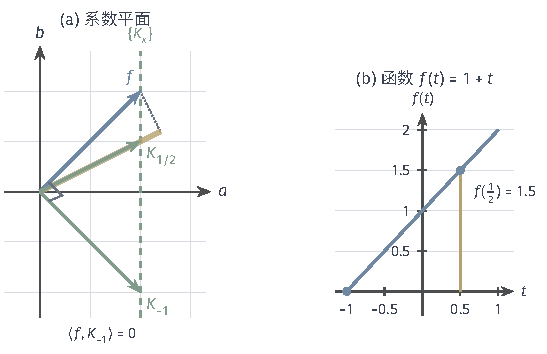
\includegraphics[width=92.7mm]{figures/02-abstract-mathematics/03-function-spaces/tikz/c5-reproducing-geometry/figure.pdf}
  \caption{仿射函数空间中再生性质的几何。(a)~系数平面$(a,b)$与空间等距；$f=1+t$对应$(1,1)$，核截面$K_x=1+xt$对应$(1,x)$，都落在虚线$a=1$上。黄色线段是$f$在$K_{1/2}$方向上的投影，其长度乘以$\|K_{1/2}\|$等于$f(1/2)=1.5$；$K_{-1}$与$f$垂直。(b)~同一函数的图像，标出$t=1/2$处的读数$1.5$与$t=-1$处的零点。}
  \label{fig:rkhs-reproducing-geometry}
\end{figure}

\paragraph{最小值核}

在$H_{\min}$中，核截面同样可以直接猜出来。式~\eqref{eq:rkhs-hmin-point-bound}的推导把$f(x)$写成了$\int_0^1f'(t)\mathbf 1_{[0,x]}(t)\,\mathrm dt$，所以只需找一个导数为$\mathbf 1_{[0,x]}$、左端取零的函数，它就是
\[
K_x(t)=\min(t,x),\qquad K(t,x)=\min(t,x)\qquad(t,x\in[0,1]).
\]
$K_x$在$[0,x]$上斜率为$1$，在$[x,1]$上保持常数$x$，确实属于$H_{\min}$，并且$\langle f,K_x\rangle_{H_{\min}}=\int_0^xf'(t)\,\mathrm dt=f(x)$。称$K(x,z)=\min(x,z)$为$[0,1]$上的\term{最小值核}（minimum kernel）。它在概率论中是标准Brown运动的协方差，但这里只把它当作一个确定的二元函数使用。

\paragraph{逐点常数与统一常数}

定义只要求每个$L_x$有界，有界常数$\|L_x\|$允许随$x$变化。在$H_{\mathrm{aff}}$中，$\|L_x\|=\|K_x\|=\sqrt{1+x^2}$。所以单位球中的函数在$x$处的取值恰好填满区间$[-\sqrt{1+x^2},\sqrt{1+x^2}]$：上界由Cauchy--Schwarz不等式给出，取$f=K_x/\|K_x\|$即可达到。

图~\ref{fig:rkhs-pointwise-envelope}画出这条包络和几条单位范数函数$\cos\theta+t\sin\theta$。每条函数在$t=\tan\theta$处与上包络相切，这正是它与$K_t$同向的位置。在整条实轴上，包络随$|t|$无限增长，不存在统一的常数$C$使$|f(t)|\le C\|f\|$对一切$t$成立；若把输入集限制为$[-1,1]$，统一常数就是$\sqrt2$。一般地，只有当$\sup_{x\in X}K(x,x)<\infty$时，核范数才能统一控制全域的点值误差：
\[
\sup_{x\in X}|f(x)-g(x)|\le\Bigl(\sup_{x\in X}\sqrt{K(x,x)}\Bigr)\,\|f-g\|_H .
\]
对$H_{\min}$，由式~\eqref{eq:rkhs-hmin-point-bound}，统一常数是$1$。

\begin{figure}[!htb]
  \centering
  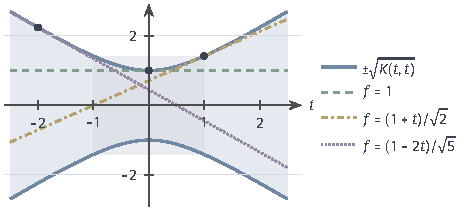
\includegraphics[width=79.6mm]{figures/02-abstract-mathematics/03-function-spaces/tikz/c5-pointwise-envelope/figure.pdf}
  \caption{仿射函数空间单位球在各点的取值范围。浅蓝区域介于$\pm\sqrt{K(t,t)}=\pm\sqrt{1+t^2}$之间；三条虚线是单位范数函数，各自在黑点处与上包络相切。灰色区域标出$[-1,1]$，其中包络的最大值为$\sqrt2$。包络在整条实轴上无界，说明逐点有界不等于统一有界。}
  \label{fig:rkhs-pointwise-envelope}
\end{figure}

\paragraph{离散空间也是RKHS}

再看一个点值有界、函数却毫无连续性的例子。对任意非空集合$X$，令$\ell^2(X)$为满足$\sum_{x\in X}f(x)^2<\infty$的函数全体（求和对至多可数个非零项进行），内积为$\sum_xf(x)g(x)$。显然$|f(x)|\le\|f\|$，所以它是RKHS，其核截面是单点示性函数$K_x=\mathbf 1_{\{x\}}$，再生核是$K(x,z)=1$（$x=z$）或$0$（$x\neq z$）。即使$X=[0,1]$，这个空间中的函数也可以在每点任意跳动。可见点值有界只是对每个固定位置的要求，函数是否随位置连续，需要核提供更多信息。

\subsection{再生核的性质}
\label{sec:rkhs-kernel-properties}

上一小节从空间得到了核。核是一个具体的二元函数，下面看它从三个方面记录空间的信息：每点读取的强弱、任意有限点组上核值矩阵的符号，以及读数随位置的变化。

\paragraph{对称性、半正定性与点值范数}

由定义式~\eqref{eq:rkhs-kernel-definition}，核值是两个核截面的内积，因此内积的性质直接转化为核的性质。

\begin{theorem}[再生核的基本性质]
\label{thm:rkhs-kernel-properties}
设$H$是$X$上的RKHS，$K$为其再生核。则：
\begin{enumerate}
\item 对称性：$K(x,z)=K(z,x)$对一切$x,z\in X$成立；
\item 半正定性：对任意$n\ge1$、任意点$x_1,\ldots,x_n\in X$与实数$a_1,\ldots,a_n$，
\[
\sum_{i,j=1}^na_ia_jK(x_i,x_j)=\Bigl\|\sum_{i=1}^na_iK_{x_i}\Bigr\|_H^2\ge0 ;
\]
\item 点值范数：$\|L_x\|=\|K_x\|_H=\sqrt{K(x,x)}$；并且对任意$x,z\in X$，$|K(x,z)|\le\sqrt{K(x,x)K(z,z)}$。
\end{enumerate}
\end{theorem}

\begin{proof}
由式~\eqref{eq:rkhs-kernel-definition}，$K(x,z)=\langle K_z,K_x\rangle$，实内积的对称性给出第1条。把$\bigl\|\sum_ia_iK_{x_i}\bigr\|^2$按双线性展开为$\sum_{i,j}a_ia_j\langle K_{x_i},K_{x_j}\rangle$，再用$\langle K_{x_i},K_{x_j}\rangle=K(x_j,x_i)=K(x_i,x_j)$，得到第2条。Riesz表示给出$\|L_x\|=\|K_x\|$，而$\|K_x\|^2=\langle K_x,K_x\rangle=K(x,x)$。最后，$|K(x,z)|=|\langle K_z,K_x\rangle|\le\|K_z\|\|K_x\|$。
\end{proof}

第2条中的矩阵$\bm G=[K(x_i,x_j)]_{i,j=1}^n$称为点组$x_1,\ldots,x_n$上的\term{Gram矩阵}或\term{核矩阵}（kernel matrix）。第2条说的就是：每个Gram矩阵都是对称半正定矩阵。这一性质不依赖于空间，只依赖于核，因此可以单独作为对二元函数的要求。

\begin{definition}[半正定核与严格正定核]
\label{def:rkhs-psd-kernel}
设$X$是非空集合。若函数$K:X\times X\to\mathbb R$对称，且对任意有限点组，其Gram矩阵都半正定，则称$K$为$X$上的半正定核，文献中也常称为\term{正定核}（positive definite kernel）。若对任意互异点$x_1,\ldots,x_n$及任意不全为零的实数$a_1,\ldots,a_n$都有$\sum_{i,j}a_ia_jK(x_i,x_j)>0$，即互异点上的Gram矩阵都可逆，则称$K$为\term{严格正定核}（strictly positive definite kernel）。
\end{definition}

“正定核”这个通行名称容易引起误解：它允许Gram矩阵奇异。本书在需要强调时写“半正定核”，与严格正定的情形区分。

\paragraph{仿射核的奇异Gram矩阵}

仿射核说明这种区分是必要的。取三个点$-1,0,1$，Gram矩阵与一个零向量为
\[
\bm G=\begin{bmatrix}2&1&0\\1&1&1\\0&1&2\end{bmatrix},\qquad
\bm G\begin{bmatrix}1\\-2\\1\end{bmatrix}=\bm 0 .
\]
对应的函数组合$K_{-1}-2K_0+K_1=(1-t)-2+(1+t)$恰好是零函数。原因很直接：$H_{\mathrm{aff}}$只有二维，任意三个核截面必然线性相关。图~\ref{fig:rkhs-gram-matrices}对五个点比较了两种核：高斯核$K(x,z)=\exp\bigl(-(x-z)^2/(2\sigma^2)\bigr)$（$\sigma=0.5$）的Gram矩阵五个特征值都为正，仿射核的Gram矩阵则只有两个正特征值$5$与$2.5$，其余三个为零。两者都是半正定核，只有前者在这个点组上可逆。

\begin{figure}[!htb]
  \centering
  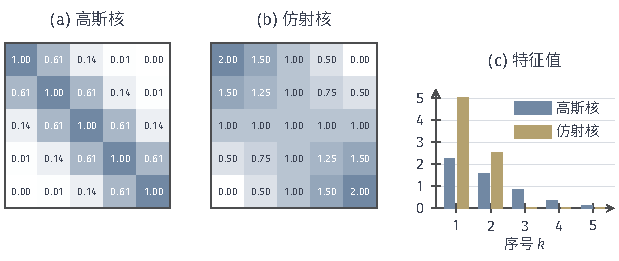
\includegraphics[width=104.8mm]{figures/02-abstract-mathematics/03-function-spaces/tikz/c5-gram-matrices/figure.pdf}
  \caption{点组$x=-1,-0.5,0,0.5,1$上的Gram矩阵。(a)~高斯核（$\sigma=0.5$），颜色越深核值越大，数字保留两位小数（右上角的$0.00$实为$e^{-8}\approx0.0003$）；(b)~仿射核$1+xz$；(c)~两个矩阵的特征值。高斯核的特征值$2.217,1.531,0.820,0.333,0.099$全为正；仿射核只有$5$与$2.5$两个正特征值，其余为零。两种核都半正定，只有前者的矩阵可逆。}
  \label{fig:rkhs-gram-matrices}
\end{figure}

高斯核在任意有限个互异实数上都给出可逆Gram矩阵，即它是严格正定核。这一结论的证明需要Fourier变换，这里不展开；本章后面用到高斯核时，只在具体计算中检查相应矩阵的可逆性。严格正定性与半正定性是两项不同的要求：半正定性可由第~\ref{sec:rkhs-kernel-operations}节的运算规则逐步验证，严格正定性则须对互异点组另行判断。

\paragraph{核截面的形状}

核截面$K_x$是$H$中的元素，所以它的形状直接展示了空间中函数的样子。图~\ref{fig:rkhs-kernel-sections}画出三种核在$[-1,1]$上的截面。高斯核的截面是以$x$为中心的钟形，离$x$越远取值越小；仿射核的截面是过点$(0,1)$的直线；二次多项式核$(1+xt)^2$的截面是抛物线。后两种核的截面都只在有限维函数族中变化，它们张成的空间分别是仿射函数与至多二次的多项式；高斯核截面则彼此不在任何有限维子空间中，这与它的严格正定性相符。

\begin{figure}[!htb]
  \centering
  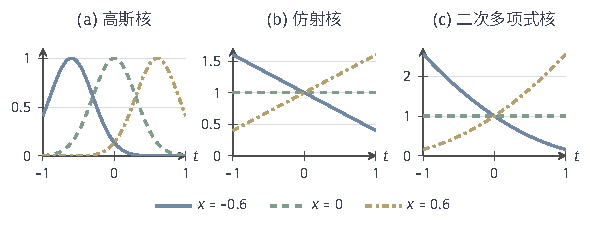
\includegraphics[width=99.9mm]{figures/02-abstract-mathematics/03-function-spaces/tikz/c5-kernel-sections/figure.pdf}
  \caption{三种核在$[-1,1]$上的核截面$K_x(t)=K(t,x)$，$x=-0.6,0,0.6$。(a)~高斯核（$\sigma=0.3$），截面是以$x$为中心的钟形；(b)~仿射核$1+xt$，截面是直线；(c)~二次多项式核$(1+xt)^2$，截面是抛物线。核截面是空间中的元素，其形状展示了空间所含函数的类型。}
  \label{fig:rkhs-kernel-sections}
\end{figure}

\paragraph{位置变化与核截面的距离}

到目前为止，每个点的读取是分开讨论的。现在固定函数$f$，只移动读取位置。由再生性质，
\[
f(x)-f(z)=\langle f,K_x-K_z\rangle_H ,
\]
所以
\begin{equation}
\begin{gathered}
|f(x)-f(z)|\le\|f\|_H\,\|K_x-K_z\|_H,\\
\|K_x-K_z\|_H^2=K(x,x)+K(z,z)-2K(x,z) .
\end{gathered}
\label{eq:rkhs-position-bound}
\end{equation}
第二个等式由展开$\langle K_x-K_z,K_x-K_z\rangle$并使用式~\eqref{eq:rkhs-kernel-definition}得到。式~\eqref{eq:rkhs-position-bound}把位置的变化转化为两个核截面在$H$中的距离，而这个距离只用核的三个值就能算出。

对三个例子分别计算这个距离。高斯核满足$K(x,x)=1$，于是$\|K_x-K_z\|^2=2-2e^{-d^2/(2\sigma^2)}$，其中$d=|x-z|$；由$1-e^{-u}\le u$得$\|K_x-K_z\|\le d/\sigma$，所以单位范数函数满足$|f(x)-f(z)|\le|x-z|/\sigma$。最小值核满足$\|K_x-K_z\|^2=x+z-2\min(x,z)=|x-z|$，于是$|f(x)-f(z)|\le\|f\|_{H_{\min}}|x-z|^{1/2}$，这正是一维Sobolev函数的$1/2$阶Hölder估计。离散空间$\ell^2(X)$的核在$x\neq z$时给出$\|K_x-K_z\|=\sqrt2$，距离不随$|x-z|$缩小。图~\ref{fig:rkhs-section-distance}把这些曲线画在一起：前两类核截面随位置连续移动，最后一类在每一点都跳开。

\begin{figure}[!htb]
  \centering
  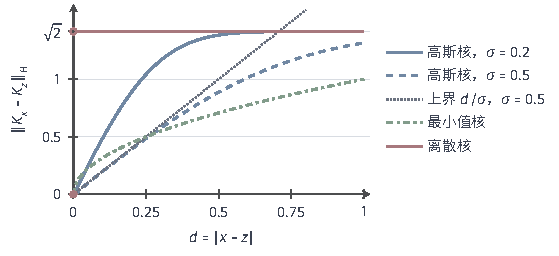
\includegraphics[width=94.7mm]{figures/02-abstract-mathematics/03-function-spaces/tikz/c5-section-distance/figure.pdf}
  \caption{核截面距离$\|K_x-K_z\|_H$随位置差$d=|x-z|$的变化。两条蓝线是高斯核（$\sigma=0.2$与$0.5$），点线是$\sigma=0.5$时的上界$d/\sigma$；绿色点划线是最小值核的$\sqrt d$；红线是离散空间$\ell^2(X)$的核，$d>0$时恒为$\sqrt2$。由式~\eqref{eq:rkhs-position-bound}，这个距离乘以$\|f\|_H$控制了$|f(x)-f(z)|$；前三条曲线在$d\to0$时趋于零，最后一条不然。}
  \label{fig:rkhs-section-distance}
\end{figure}

\paragraph{连续核与函数的连续性}

上述计算可以整理成一条一般结论。

\begin{theorem}[连续核给出连续函数]
\label{thm:rkhs-continuity}
设$X$是度量空间，$H$是$X$上的RKHS，再生核$K$在$X\times X$上连续。则：
\begin{enumerate}
\item 映射$x\mapsto K_x$从$X$到$H$连续，因而每个$f\in H$都是$X$上的连续函数；
\item 若$X$还是紧的，则对任意$R>0$，球$B_R=\{f\in H:\|f\|_H\le R\}$中的函数一致有界且等度连续：对任意$\varepsilon>0$存在$\delta>0$，使得$d(x,z)<\delta$时，对一切$f\in B_R$都有$|f(x)-f(z)|<\varepsilon$。
\end{enumerate}
\end{theorem}

\begin{proof}
当$z\to x$时，$K$的连续性使$K(z,z)\to K(x,x)$、$K(x,z)\to K(x,x)$，由式~\eqref{eq:rkhs-position-bound}的第二个等式得$\|K_x-K_z\|\to0$；再由第一个不等式，$f(z)\to f(x)$。这证明第1条。

若$X$紧，则$X\times X$紧，连续函数$K$一致连续（第~\ref{sec:metric-compact-continuous}节），并且对角线上的$K(x,x)$有最大值$M^2$。一致连续性给出：对任意$\eta>0$存在$\delta>0$，使得$d(x,z)<\delta$时$K(x,x)+K(z,z)-2K(x,z)<\eta$。取$\eta=(\varepsilon/R)^2$，式~\eqref{eq:rkhs-position-bound}便对$B_R$中所有$f$同时给出$|f(x)-f(z)|<\varepsilon$；一致有界性来自$|f(x)|\le M\|f\|\le MR$。
\end{proof}

第2条中的$\delta$只依赖于核与半径$R$，不依赖于球中具体的函数，这是“共同的连续性控制”的含义。第~\ref{sec:apx-arzela-ascoli}节将用这种一致有界、等度连续的性质判断函数族的紧性。还要强调两种稳定性的区别：固定位置时，$|f(x)-g(x)|\le\sqrt{K(x,x)}\|f-g\|_H$描述函数改变引起的读数改变；固定函数时，式~\eqref{eq:rkhs-position-bound}描述位置改变引起的读数改变。离散空间$\ell^2([0,1])$说明前者成立并不蕴含后者。

% 第5章第2节：核与函数空间的构造（从半正定核构造空间、特征映射、核的运算）。

\section{核与函数空间的构造}
\label{sec:rkhs-construction}

上一节从空间出发得到了核，并看到每个再生核都是半正定核。本节回答反方向的问题：只给定集合$X$上的一个半正定核，能否找到以它为再生核的函数空间，这个空间是否唯一。第~\ref{sec:rkhs-from-kernel}节用核截面的有限组合、商去零长度方向和完备化三步给出一般构造。一般构造虽然完整，却不便于检验一个具体的二元函数是否半正定，所以后两小节给出两种可操作的办法：把核写成特征向量的内积，或者由已知的核经运算得到新核。这些步骤都只用到集合与核，不需要预先给定测度。

\subsection{从半正定核构造空间}
\label{sec:rkhs-from-kernel}

设$K$是非空集合$X$上的半正定核。如果以$K$为再生核的空间存在，它一定含有全部核截面$K_x$，并且核截面之间的内积必须是$\langle K_x,K_z\rangle=K(z,x)$。构造就从这两点出发。

\paragraph{有限核和与它们的内积}

令$H_0=\operatorname{span}\{K_x:x\in X\}$，它由有限和$f=\sum_{i=1}^na_iK_{x_i}$组成，每个元素都是$X$上的真实函数$f(t)=\sum_ia_iK(t,x_i)$。对$f=\sum_ia_iK_{x_i}$与$g=\sum_jb_jK_{z_j}$，按照上述要求定义
\begin{equation}
\langle f,g\rangle_0=\sum_{i,j}a_ib_jK(z_j,x_i).
\label{eq:rkhs-h0-inner}
\end{equation}

同一个函数可以有多种有限和表示，必须先检查式~\eqref{eq:rkhs-h0-inner}与表示的选取无关。对$j$先求和内层的$i$，得到$\langle f,g\rangle_0=\sum_jb_jf(z_j)$，它只依赖于$f$作为函数的取值；由$K$的对称性，同一个量也等于$\sum_ia_ig(x_i)$，只依赖于$g$的取值。于是换掉$f$的表示不改变第一种写法，换掉$g$的表示不改变第二种写法，$\langle f,g\rangle_0$良定义。它显然对称、双线性，且$\langle f,f\rangle_0=\bm a^{\top}\bm G\bm a\ge0$，其中$\bm G$是点组$x_1,\ldots,x_n$上的Gram矩阵。取$g=K_x$，由第一种写法立刻得到
\begin{equation}
\langle f,K_x\rangle_0=f(x)\qquad(f\in H_0),
\label{eq:rkhs-h0-reproducing}
\end{equation}
即再生性质在$H_0$上已经成立。

\paragraph{零长度方向}

若把系数向量$\bm a$本身当作对象，二次型$\bm a^{\top}\bm G\bm a$只是半正定的，可能对非零$\bm a$取零。第~\ref{sec:rkhs-kernel-properties}节的仿射核例子中，点$-1,0,1$上的系数$(1,-2,1)$长度为零。所以不能直接把系数空间连同这个二次型当作内积空间，必须先商去零长度的方向。

把系数映成函数，恰好完成了这个商。Cauchy--Schwarz不等式的证明只用到半正定性与双线性，对$\langle\cdot,\cdot\rangle_0$同样成立，结合式~\eqref{eq:rkhs-h0-reproducing}得
\begin{equation}
|f(x)|=|\langle f,K_x\rangle_0|\le\sqrt{K(x,x)}\,\|f\|_0 .
\label{eq:rkhs-h0-point-bound}
\end{equation}
所以长度为零的组合在每一点取零，是零函数；反过来，零函数$f$满足$\langle f,f\rangle_0=\sum_ia_if(x_i)=0$。零长度的系数组合恰好就是给出零函数的组合。在仿射核的例子中，$K_{-1}-2K_0+K_1$正是零函数。因此在函数空间$H_0$上，$\langle\cdot,\cdot\rangle_0$已经是真正的内积。

\paragraph{完备化与点值的极限}

$H_0$一般不完备。为得到Hilbert空间，取$H_0$的完备化$\overline{H_0}$：由定理~\ref{thm:metric-completion}，它由$H_0$中Cauchy列的等价类组成，内积可以由连续性延拓过去（第~\ref{sec:fs-hilbert}节）。但完备化中的元素是抽象的等价类，还不是$X$上的函数，接下来要把它们变回函数。

点值估计~\eqref{eq:rkhs-h0-point-bound}正好提供了这一步。若$(f_n)$是$H_0$中的Cauchy列，则$|f_n(x)-f_m(x)|\le\sqrt{K(x,x)}\|f_n-f_m\|_0$，所以在每一点$f_n(x)$都是Cauchy数列，有确定的极限；等价的Cauchy列相差一列趋于零的函数，在每一点有相同的极限。用内积表达，就是定义
\[
J:\overline{H_0}\to\{X\text{上的实函数}\},\qquad (J\xi)(x)=\langle\xi,K_x\rangle_{\overline{H_0}} .
\]
若$f_n\to\xi$，则$f_n(x)=\langle f_n,K_x\rangle\to(J\xi)(x)$，所以$J\xi$就是逼近$\xi$的Cauchy列的逐点极限；由式~\eqref{eq:rkhs-h0-reproducing}，$J$在$H_0$上是恒等映射。

\paragraph{排除额外的零方向}

还剩一个危险：$\overline{H_0}$中两个不同的元素，会不会给出同一个函数？若是这样，函数之间就无法定义内积。等价地，要排除这样的$\xi\neq0$：$J\xi$是零函数。这一步要用到核截面在$\overline{H_0}$中稠密。若$(J\xi)(x)=\langle\xi,K_x\rangle=0$对一切$x$成立，则$\xi$与每个$K_x$正交，从而与它们的张成$H_0$正交；$H_0$在$\overline{H_0}$中稠密，所以$\xi$与整个空间正交，$\xi=0$。因此$J$是单射。

\begin{theorem}[由半正定核确定再生核Hilbert空间]
\label{thm:rkhs-moore-aronszajn}
设$K$是非空集合$X$上的半正定核。则存在唯一的RKHS，记为$H_K$，以$K$为其再生核。并且有限核和全体$H_0=\operatorname{span}\{K_x:x\in X\}$在$H_K$中稠密，$H_K$的每个元素都是$H_0$中某个Cauchy列的逐点极限。
\end{theorem}

\begin{proof}
存在性。令$H_K=J(\overline{H_0})$，并规定$\langle J\xi,J\eta\rangle_{H_K}=\langle\xi,\eta\rangle_{\overline{H_0}}$。由于$J$是线性单射，这个定义良好，且$J$成为从$\overline{H_0}$到$H_K$的等距同构，所以$H_K$是Hilbert空间；$J$的线性说明$H_K$中的加法和数乘就是逐点运算。$J$在$H_0$上是恒等映射，故$K_x=JK_x\in H_K$，并且对$f=J\xi$有
\[
f(x)=\langle\xi,K_x\rangle_{\overline{H_0}}=\langle J\xi,JK_x\rangle_{H_K}=\langle f,K_x\rangle_{H_K} .
\]
这就是以$K$为再生核的再生性质，点值有界随之成立。稠密性与逐点极限的描述来自$H_0$在$\overline{H_0}$中稠密以及上一段关于$J$的讨论。

唯一性。设$H$是另一个以$K$为再生核的RKHS。$H$含有每个$K_x$，且$\langle K_x,K_z\rangle_H=K(z,x)$，所以$H_0\subseteq H$，两者在$H_0$上的内积一致。$H_0$在$H$中也稠密：若$f\in H$与每个$K_x$正交，则由再生性质$f(x)=0$对一切$x$成立。任取$f\in H$及$H_0$中的序列$f_n\to f$（按$H$的范数），$(f_n)$是$H_0$中的Cauchy列，再生性质说明它逐点收敛到$f$；同一序列在$H_K$中收敛到其逐点极限，即$f$。所以$f\in H_K$且$\|f\|_{H_K}=\lim\|f_n\|=\|f\|_H$。对调两个空间的角色，得$H=H_K$，且范数相同。
\end{proof}

这条结论通常称为Moore--Aronszajn定理\scite{aronszajn1950kernels}。图~\ref{fig:rkhs-construction-steps}概括了四个阶段：系数组合上只有半内积；变为函数后零长度方向被商去；完备化补上极限；点值读取把极限元素重新表示为函数，核截面的稠密性保证这种表示是单射。

\begin{figure}[!htb]
  \centering
  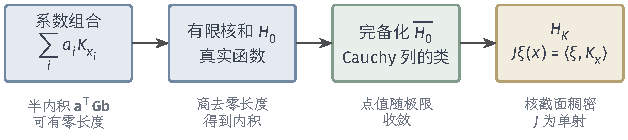
\includegraphics[width=106.4mm]{figures/02-abstract-mathematics/03-function-spaces/tikz/c5-construction-steps/figure.pdf}
  \caption{由半正定核构造$H_K$的四个阶段。系数组合上的二次型$\bm a^{\top}\bm G\bm b$只是半内积，可能有零长度方向；把组合看成函数便商去了这些方向，得到内积空间$H_0$；完备化$\overline{H_0}$的元素是Cauchy列的类，点值估计使它们的点值随极限收敛；映射$J$把它们表示为函数，核截面稠密保证$J$为单射。}
  \label{fig:rkhs-construction-steps}
\end{figure}

\paragraph{由最小值核重建$H_{\min}$}

以最小值核为例走一遍构造。$H_0$由$\min(\cdot,x_j)$的有限组合组成，即在$[0,1]$上连续、分段线性、左端为零、在最右节点之后保持常数的函数。核截面的内积可以写成导数的积分：
\[
\langle K_x,K_z\rangle_0=\min(x,z)=\int_0^1\mathbf 1_{[0,x]}(t)\mathbf 1_{[0,z]}(t)\,\mathrm dt=\int_0^1K_x'(t)K_z'(t)\,\mathrm dt ,
\]
所以在$H_0$上$\|f\|_0=\|f'\|_{L^2}$。$H_0$中函数的导数恰好是阶梯函数，而区间上的阶梯函数在$L^2(0,1)$中稠密（第~\ref{sec:fs-density-separability}节），于是完备化后得到的空间经由$f\mapsto f'$与$L^2(0,1)$等距同构，它就是第~\ref{sec:rkhs-reproducing}节的$H_{\min}$。$H_0$本身不完备：例如$f(t)=t-t^2/2$属于$H_{\min}$，却不是分段线性函数，它只是$H_0$中一列折线的极限。

这个例子也说明了唯一性的用处：我们已经知道$H_{\min}$是以$\min(x,z)$为再生核的RKHS，定理~\ref{thm:rkhs-moore-aronszajn}立刻保证从核出发构造的空间就是它，不必另作比较。

\paragraph{构造用到了什么}

整个构造只用到集合$X$与核的半正定性，没有测度，也不要求$X$带有拓扑。所得的稠密性是在核范数意义下：$H_K$中的每个函数都能被有限核和按$\|\cdot\|_{H_K}$逼近，因而也被逐点逼近。这并没有回答有限核和能否逼近$H_K$之外的函数，例如$[0,1]$上任意给定的连续函数；那是第~\ref{sec:apx-kernel-sections}节要讨论的问题，答案取决于具体的核。

\subsection{特征映射}
\label{sec:rkhs-feature-maps}

一般构造告诉我们半正定核总对应一个空间，但要验证某个二元函数半正定，逐一检查所有Gram矩阵并不现实。最常用的办法是把核写成两个向量的内积。

\paragraph{有限特征向量的内积核}

设$\Phi:X\to\mathbb R^d$，令$K(x,z)=\Phi(x)^{\top}\Phi(z)$。对任意点组与系数，
\[
\sum_{i,j}a_ia_jK(x_i,x_j)=\Bigl\|\sum_ia_i\Phi(x_i)\Bigr\|_2^2\ge0 ,
\]
所以$K$是半正定核；用矩阵写，Gram矩阵等于$\bm\Phi\bm\Phi^{\top}$，其中$\bm\Phi$的第$i$行是$\Phi(x_i)^{\top}$。例如，对实数$x,z$，
\[
(1+xz)^2=1+2xz+x^2z^2=\bigl\langle(1,\sqrt2\,x,x^2),\ (1,\sqrt2\,z,z^2)\bigr\rangle ,
\]
所以二次多项式核是三维特征向量的内积核。

\paragraph{一般特征映射}

有限维的要求可以去掉。

\begin{definition}[特征映射]
\label{def:rkhs-feature-map}
设$X$是非空集合，$\mathcal F$是实Hilbert空间，$\Phi:X\to\mathcal F$是任意映射。若$K(x,z)=\langle\Phi(x),\Phi(z)\rangle_{\mathcal F}$，则称$\Phi$为$K$的一个\term{特征映射}（feature map），$\mathcal F$为相应的特征空间。
\end{definition}

与有限维情形完全相同的计算说明，任何特征映射给出的$K$都是半正定核。反过来，每个半正定核都有特征映射：取$\mathcal F=H_K$、$\Phi(x)=K_x$，则$\langle K_x,K_z\rangle_{H_K}=K(x,z)$。称它为\term{规范特征映射}（canonical feature map）。所以“$K$半正定”与“$K$有某个特征映射”是等价的。

同一个核可以有许多不同的特征映射。仿射核$1+xz$既可以写成$\Phi_1(x)=(1,x)\in\mathbb R^2$的内积，也可以写成$\Phi_2(x)=(1,x/\sqrt2,x/\sqrt2)\in\mathbb R^3$的内积，因为$1+\tfrac{x z}{2}+\tfrac{xz}{2}=1+xz$。特征空间的维数和坐标都可以不同，核却相同，因此由核确定的空间也相同。下面说明这个空间怎样从任何一个特征映射读出来。

\paragraph{参数表示与可见子空间}

给定特征映射$\Phi:X\to\mathcal F$，每个参数$w\in\mathcal F$确定一个函数
\[
f_w(x)=\langle w,\Phi(x)\rangle_{\mathcal F}.
\]
令$V=\overline{\operatorname{span}}\{\Phi(x):x\in X\}$为特征值张成的闭子空间，$P_V$为到$V$的正交投影。由于$w-P_Vw$与每个$\Phi(x)$正交，$f_w=f_{P_Vw}$：正交补$V^\perp$中的参数分量不影响函数。称$V$为可见参数子空间。

\begin{theorem}[特征映射给出的RKHS]
\label{thm:rkhs-feature-space}
设$\Phi:X\to\mathcal F$是半正定核$K$的特征映射，$V$为特征值张成的闭子空间。则
\[
H_K=\{f_w:w\in\mathcal F\},\qquad
\|f_w\|_{H_K}=\|P_Vw\|_{\mathcal F}=\min_{u\in\mathcal F,\ f_u=f_w}\|u\|_{\mathcal F} ,
\]
并且$w\mapsto f_w$限制在$V$上是从$V$到$H_K$的等距同构。
\end{theorem}

\begin{proof}
线性映射$A:w\mapsto f_w$的核是$\{w:\langle w,\Phi(x)\rangle=0,\ \forall x\}=V^\perp$，所以$A$在$V$上是单射。令$H=A(\mathcal F)=A(V)$，并规定$\|Aw\|_H=\|P_Vw\|$，则$A|_V$是等距同构，$H$作为闭子空间$V$的等距像是Hilbert空间，运算是逐点的。

点值有界：$|f_w(x)|=|\langle P_Vw,\Phi(x)\rangle|\le\|\Phi(x)\|\,\|f_w\|_H$。再生核：令$k_x=A\Phi(x)$，因$\Phi(x)\in V$，有$\langle f_w,k_x\rangle_H=\langle P_Vw,\Phi(x)\rangle=f_w(x)$；而$k_x(z)=\langle\Phi(x),\Phi(z)\rangle=K(z,x)$，即$k_x=K_x$。所以$H$是以$K$为再生核的RKHS，由定理~\ref{thm:rkhs-moore-aronszajn}的唯一性，$H=H_K$。最后，$f_u=f_w$当且仅当$u-w\in V^\perp$，此时$P_Vu=P_Vw$，而$\|u\|\ge\|P_Vu\|$，等号在$u\in V$时取得。
\end{proof}

定理的最后一个等式提醒我们：在冗余的特征表示中，任意一个能给出$f$的参数$w$，其范数只是$\|f\|_{H_K}$的上界；只有落在可见子空间中的那一个参数，范数才等于函数的范数。

\paragraph{冗余特征的例子}

取$\Phi(x)=(x,x)\in\mathbb R^2$，核为$K(x,z)=2xz$。可见子空间是直线$V=\operatorname{span}\{(1,1)\}$，正交补方向是$(1,-1)$。参数$(2,0)$、$(1,1)$、$(0,2)$都给出同一函数$f(x)=2x$，范数分别为$2$、$\sqrt2$、$2$；由定理~\ref{thm:rkhs-feature-space}，$\|f\|_{H_K}=\sqrt2$，它是$(2,0)$在$V$上的投影$(1,1)$的长度，见图~\ref{fig:rkhs-visible-parameters}。直接检验：$H_K$由$f(x)=cx$组成，核截面$K_x(t)=2xt$，再生性质要求$\langle ct,2xt\rangle=cx$，故$\langle ct,c't\rangle_{H_K}=cc'/2$，$\|2x\|_{H_K}^2=4/2=2$，结果一致。

对仿射核的两个特征映射，$\Phi_1$的可见子空间是整个$\mathbb R^2$（$\Phi_1(-1)$与$\Phi_1(1)$线性无关），所以$\|a+bt\|_{H_K}^2=a^2+b^2$，与第~\ref{sec:rkhs-reproducing}节一致。$\Phi_2$的可见子空间是$\operatorname{span}\{(1,0,0),(0,1,1)/\sqrt2\}$，参数$(a,b/\sqrt2,b/\sqrt2)$给出$a+bt$，长度同样是$\sqrt{a^2+b^2}$；而参数$(a,\sqrt2 b,0)$给出同一函数，长度$\sqrt{a^2+2b^2}$却更大。

\begin{figure}[!htb]
  \centering
  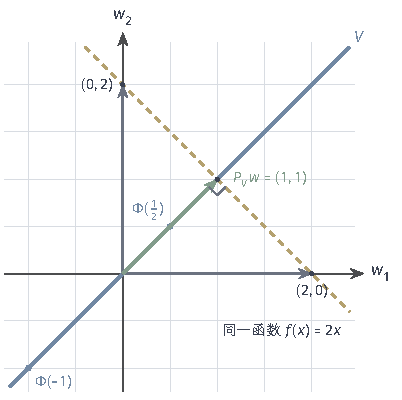
\includegraphics[width=68.1mm]{figures/02-abstract-mathematics/03-function-spaces/tikz/c5-visible-parameters/figure.pdf}
  \caption{冗余特征$\Phi(x)=(x,x)$的参数平面。特征值$\Phi(x)$都落在蓝色直线$V$上；黄色虚线上的参数都给出同一函数$f(x)=2x$。其中与$V$相交的$P_Vw=(1,1)$长度最短，为$\sqrt2$，这就是$\|f\|_{H_K}$；$(2,0)$与$(0,2)$长度为$2$，多出的部分来自对函数没有影响的$V^\perp$方向。}
  \label{fig:rkhs-visible-parameters}
\end{figure}

\subsection{核的运算}
\label{sec:rkhs-kernel-operations}

特征映射适合验证可以写成内积的核。更多的核是由几种基本核经过加法、乘法和换输入等运算得到的；只要这些运算保持半正定性，就不必为每个新核重新寻找特征映射。

\paragraph{保持半正定性的运算}

\begin{theorem}[核的运算]
\label{thm:rkhs-kernel-operations}
设$K_1,K_2$是非空集合$X$上的半正定核。则下列函数都是半正定核：
\begin{enumerate}
\item 非负线性组合$\alpha K_1+\beta K_2$，其中$\alpha,\beta\ge0$；
\item 逐点乘积$K_1(x,z)K_2(x,z)$；
\item 换输入：对任意集合$Y$和映射$\varphi:Y\to X$，$Y$上的$K_1(\varphi(y),\varphi(y'))$；
\item 函数缩放：对任意$g:X\to\mathbb R$，$g(x)g(z)K_1(x,z)$；
\item 逐点极限：若半正定核$K^{(n)}$在每个$(x,z)$处收敛到$K(x,z)$，则$K$半正定。
\end{enumerate}
\end{theorem}

\begin{proof}
固定点组$x_1,\ldots,x_n$与系数向量$\bm c$，记$\bm G_1,\bm G_2$为两个核的Gram矩阵。第1条：$\bm c^{\top}(\alpha\bm G_1+\beta\bm G_2)\bm c=\alpha\bm c^{\top}\bm G_1\bm c+\beta\bm c^{\top}\bm G_2\bm c\ge0$；用特征映射表达，把$\sqrt\alpha\,\Phi_1(x)$与$\sqrt\beta\,\Phi_2(x)$拼接成直和空间中的一个向量即可。

第2条：乘积核的Gram矩阵是逐元素乘积$\bm G_1\odot\bm G_2$。半正定矩阵$\bm G_2$可分解为$\bm G_2=\bm B\bm B^{\top}$（例如由谱分解取$\bm B=\bm U\bm\Lambda^{1/2}$），记$\bm b_k$为$\bm B$的第$k$列，则
\[
\bm c^{\top}(\bm G_1\odot\bm G_2)\bm c
=\sum_{i,j}c_ic_j(\bm G_1)_{i,j}\sum_k\bm B_{i,k}\bm B_{j,k}
=\sum_k(\bm c\odot\bm b_k)^{\top}\bm G_1(\bm c\odot\bm b_k)\ge0 .
\]
这就是Schur乘积定理。若两个核分别有有限维特征映射，乘积核的特征映射是张量积$\Phi_1(x)\otimes\Phi_2(x)$，因为$\langle u\otimes v,u'\otimes v'\rangle=\langle u,u'\rangle\langle v,v'\rangle$。

第3条：点组$y_1,\ldots,y_n$上的Gram矩阵就是点组$\varphi(y_1),\ldots,\varphi(y_n)$上$K_1$的Gram矩阵（允许点重复）。第4条：二次型等于$(\bm c\odot\bm g)^{\top}\bm G_1(\bm c\odot\bm g)$，其中$\bm g=(g(x_1),\ldots,g(x_n))$。第5条：每个二次型$\bm c^{\top}\bm G^{(n)}\bm c$非负，有限和的极限仍非负。
\end{proof}

逐元素乘积的半正定性和张量积的内积公式都是有限维线性代数中的结论，可参考\BookChapterRef{chap:normed-inner-product-spaces}{卷一《数学准备：基础数学》“赋范空间与内积空间”章中的Gram矩阵与Schur乘积}及\BookChapterRef{chap:linear-operations}{卷一“向量、矩阵与张量的运算”章中的张量积}。这里只用到它们在有限点组上的形式。

\paragraph{线性核、多项式核与高斯核}

由这几条规则可以验证常用的核。在$\mathbb R^d$上，\term{线性核}$K(\bm x,\bm z)=\bm x^{\top}\bm z$以$\Phi(\bm x)=\bm x$为特征映射。常数$c\ge0$是以$\sqrt c$为特征的核，于是$c+\bm x^{\top}\bm z$半正定（第1条），它的$p$次幂即\term{多项式核}$(c+\bm x^{\top}\bm z)^p$也半正定（第2条反复使用）。

\term{高斯核}（Gaussian kernel）$K_\sigma(\bm x,\bm z)=\exp\bigl(-\|\bm x-\bm z\|_2^2/(2\sigma^2)\bigr)$分三步验证。先把指数中的平方展开：
\[
\exp\Bigl(-\frac{\|\bm x-\bm z\|_2^2}{2\sigma^2}\Bigr)
=g(\bm x)\,g(\bm z)\,\exp\Bigl(\frac{\bm x^{\top}\bm z}{\sigma^2}\Bigr),\qquad
g(\bm x)=\exp\Bigl(-\frac{\|\bm x\|_2^2}{2\sigma^2}\Bigr).
\]
再看中间的因子：对每个$N$，部分和$\sum_{k=0}^N(\bm x^{\top}\bm z)^k/(k!\,\sigma^{2k})$是线性核的幂的非负组合，因而半正定；指数级数在每一点收敛，由第5条，极限$\exp(\bm x^{\top}\bm z/\sigma^2)$半正定。最后由第4条乘上$g(\bm x)g(\bm z)$。

\paragraph{运算在核截面上的效果}

核运算直接作用在核截面上：和核的截面是两个截面之和，乘积核的截面是两个截面之积。图~\ref{fig:rkhs-kernel-operations}在$x=0.4$处比较仿射核与高斯核（$\sigma=0.3$）。和核的截面在仿射趋势上叠加了一个局部隆起；乘积核的截面仍集中在$x$附近，但被仿射因子$1+0.4t$拉得右高左低。这说明乘积核所对应空间中的函数同时带有两种核的特点：局部性来自高斯因子，倾斜来自仿射因子。

\begin{figure}[!htb]
  \centering
  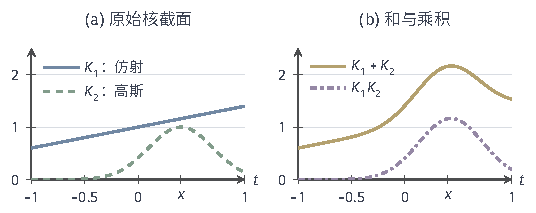
\includegraphics[width=90.7mm]{figures/02-abstract-mathematics/03-function-spaces/tikz/c5-kernel-operations/figure.pdf}
  \caption{核运算在核截面上的效果，固定$x=0.4$，$t\in[-1,1]$。(a)~仿射核截面$1+0.4t$与高斯核截面（$\sigma=0.3$）；(b)~两者之和与逐点乘积。和核的截面是两个截面相加，乘积核的截面是两个截面相乘，仍保持以$x$为中心的局部形状。}
  \label{fig:rkhs-kernel-operations}
\end{figure}

\paragraph{半正定性给不出的结论}

上面的规则只涉及非负组合、乘积与极限，减法不在其中。两个半正定核之差一般不是半正定核：仿射核减去常数核$2$得到$xz-1$，它在$x=z=0$处的对角值为$-1$，而半正定核的对角值$K(x,x)$必须非负。

半正定性也不包含更强的性质。二次多项式核$(1+xz)^2$在$\mathbb R$上半正定，但由特征映射$(1,\sqrt2x,x^2)$与定理~\ref{thm:rkhs-feature-space}，它的RKHS就是至多二次的多项式全体，任意四个点上的Gram矩阵都奇异，所以它不是严格正定核。这个三维空间在$C[-1,1]$中是闭的，不能一致逼近$|x|$这样的连续函数。高斯核既严格正定，又能用有限核和逼近紧区间上的任意连续函数，但后一性质需要第~\ref{sec:apx-kernel-sections}节专门的稠密性论证，不能从半正定性推出。

% 第5章第3节：有限观测与核表示（观测确定的函数子空间、有限中心的投影表示）。

\section{有限观测与核表示}
\label{sec:rkhs-finite-observations}

回到章首的传感器问题：我们只在有限个位置读到函数值。第~\ref{sec:lfo-finite-observations}节在有限维候选空间中讨论过一般线性观测，把每条读取规则写成观测矩阵的一行；那里的关键条件是观测在候选空间上满列秩。RKHS通常是无限维的，有限个读数不可能确定整个函数，问题于是变成：读数究竟确定了函数的哪一部分？由再生性质，每个点值读取都是与一个核截面的内积，所以答案可以用核截面张成的子空间和正交投影完整写出。本节先说明读数看见与看不见的方向，再把投影写成核矩阵方程，并讨论读数之外的误差和由观测点得到的有限维核。

\subsection{观测确定的函数子空间}
\label{sec:rkhs-observed-subspace}

固定RKHS $H$及其再生核$K$，取互异的观测位置$Z=\{x_1,\ldots,x_n\}\subseteq X$。对$f\in H$，读数向量是$\bm b=(f(x_1),\ldots,f(x_n))^{\top}$。

\paragraph{观测子空间与余项}

由再生性质，$f(x_i)=\langle f,K_{x_i}\rangle$，读数只与$f$在核截面$K_{x_1},\ldots,K_{x_n}$上的内积有关。令
\[
M_Z=\operatorname{span}\{K_{x_1},\ldots,K_{x_n}\},
\]
它是有限维子空间，因而是闭的。记$P=P_{M_Z}$为到$M_Z$的正交投影（第~\ref{sec:fs-projection}节），把$f$分解为$f=Pf+r$，其中$r\perp M_Z$。余项与每个$K_{x_i}$正交，正是说$r(x_i)=\langle r,K_{x_i}\rangle=0$。

\begin{theorem}[观测子空间]
\label{thm:rkhs-observed-subspace}
在上述记号下，$M_Z^\perp=\{g\in H:g(x_1)=\cdots=g(x_n)=0\}$。对$f,g\in H$，下列三条等价：$f$与$g$在$Z$上读数相同；$f-g\in M_Z^\perp$；$Pf=Pg$。
\end{theorem}

\begin{proof}
$g\perp M_Z$当且仅当$g$与每个$K_{x_i}$正交，即$g(x_i)=0$对每个$i$成立，这给出第一个等式。$f$与$g$读数相同，当且仅当$f-g$在每个$x_i$处取零，即$f-g\in M_Z^\perp$。由$H=M_Z\oplus M_Z^\perp$，$f-g\in M_Z^\perp$当且仅当$P(f-g)=0$。
\end{proof}

所以有限个点值恰好确定投影$Pf$，余项$r$则完全看不见：它在每个观测点取零，不论多大都不会改变任何读数。图~\ref{fig:rkhs-observation-residual}给出一个具体例子。取$[0,1]$上$\sigma=0.15$的高斯核，目标$f=K_{0.2}-0.8K_{0.5}+0.9K_{0.8}$，观测点$x_1,\ldots,x_4=0.1,0.35,0.6,0.9$。投影$Pf$与$f$在四个观测点重合，在观测点之间却可以明显不同；余项$r=f-Pf$在观测点处为零，在两点之间的振幅达到$0.41$。按范数计算，$\|f\|_H^2=2.039$，其中$\|Pf\|_H^2=1.210$被观测看见，其余$\|r\|_H^2=0.829$完全看不见。

\begin{figure}[!htb]
  \centering
  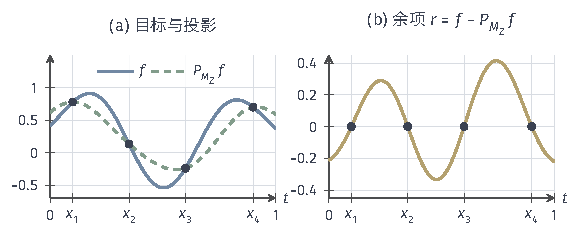
\includegraphics[width=97.9mm]{figures/02-abstract-mathematics/03-function-spaces/tikz/c5-observation-residual/figure.pdf}
  \caption{高斯核（$\sigma=0.15$）空间中的观测投影。(a)~目标$f=K_{0.2}-0.8K_{0.5}+0.9K_{0.8}$（实线）与它在$M_Z=\operatorname{span}\{K_{x_1},\ldots,K_{x_4}\}$上的投影（虚线），观测点$x_i=0.1,0.35,0.6,0.9$处两者取值相同（黑点）；(b)~余项$r=f-P_{M_Z}f$在每个观测点为零。读数只确定投影，余项对读数没有任何影响。}
  \label{fig:rkhs-observation-residual}
\end{figure}

\paragraph{Gram矩阵、读数与范数}

$M_Z$中的元素都能写成$g=\sum_ja_jK_{x_j}$，它的读数和范数都可以用Gram矩阵$\bm G_{i,j}=K(x_i,x_j)$计算：
\begin{equation}
\begin{gathered}
g(x_i)=\sum_ja_jK(x_i,x_j)=(\bm G\bm a)_i,\qquad
\|g\|_H^2=\bm a^{\top}\bm G\bm a,\\
\Bigl\langle\sum_ja_jK_{x_j},\sum_jc_jK_{x_j}\Bigr\rangle_H=\bm a^{\top}\bm G\bm c .
\end{gathered}
\label{eq:rkhs-gram-calculus}
\end{equation}
因此在$M_Z$内部，函数的全部计算都化为$n$维向量与$n\times n$矩阵的计算。注意$\bm a^{\top}\bm G\bm a$才是函数的范数平方，系数向量的欧氏长度$\|\bm a\|_2$一般与函数范数无关。

\paragraph{系数的不唯一与函数的不唯一}

有限观测下有两种不同的不唯一，它们来自不同的地方。第一种是系数的不唯一：两个系数向量$\bm a,\bm a'$给出同一个函数，当且仅当$\bigl\|\sum_j(a_j-a_j')K_{x_j}\bigr\|^2=(\bm a-\bm a')^{\top}\bm G(\bm a-\bm a')=0$，对半正定矩阵这等价于$\bm G(\bm a-\bm a')=\bm 0$。所以系数的冗余由$\ker\bm G$描述，它只是同一函数的不同写法。第二种是函数的不唯一：读数相同的函数可以相差$M_Z^\perp$中的任意元素，它们是真正不同的函数。

两个例子说明这两种情况互不决定。在仿射空间$H_{\mathrm{aff}}$中取$Z=\{-1,0,1\}$，第~\ref{sec:rkhs-kernel-properties}节已算出$\ker\bm G=\operatorname{span}\{(1,-2,1)\}$，系数不唯一；但三个核截面已经张成整个二维空间，$M_Z^\perp=\{0\}$，读数唯一确定函数。在$H_{\min}$中取$Z=\{1/3,2/3,1\}$，Gram矩阵
\[
\bm G=\frac13\begin{bmatrix}1&1&1\\1&2&2\\1&2&3\end{bmatrix},\qquad
\det\bm G=\frac1{27},
\]
可逆，系数唯一；但$M_Z^\perp$由在这三点取零的$H_{\min}$函数组成，是无限维的，读数远不能确定函数。若$K$严格正定，互异点上的Gram矩阵总可逆，第一种不唯一不会出现，第二种在无限维空间中却总是存在。

\subsection{有限中心的投影表示}
\label{sec:rkhs-center-projection}

上一小节说明读数确定$Pf$。现在把$Pf$实际算出来，即求出它在核截面$K_{x_1},\ldots,K_{x_n}$上的系数；这些观测位置在表示中充当中心。

\paragraph{正交条件与核矩阵方程}

设$Pf=\sum_ja_jK_{x_j}$。投影由正交条件$\langle f-Pf,K_{x_i}\rangle=0$（$i=1,\ldots,n$）刻画，由再生性质，它就是$(Pf)(x_i)=f(x_i)$，再由式~\eqref{eq:rkhs-gram-calculus}，
\begin{equation}
\bm G\bm a=\bm b,\qquad \bm b_i=f(x_i).
\label{eq:rkhs-center-equation}
\end{equation}
投影的正交条件与“在观测点插值”在这里是同一组方程。

\begin{theorem}[有限中心的投影]
\label{thm:rkhs-center-projection}
设$\bm b$是某个$f\in H$在$Z$上的读数。则：
\begin{enumerate}
\item 方程~\eqref{eq:rkhs-center-equation}有解，任意一个解$\bm a$都给出同一个函数$\sum_ja_jK_{x_j}=Pf$；
\item $Pf$是$M_Z$中唯一在$Z$上取读数$\bm b$的函数，也是$H$中所有满足$g(x_i)=\bm b_i$的函数$g$里范数最小的一个，且$\|Pf\|_H^2=\bm b^{\top}\bm a=\bm b^{\top}\bm G^{\dagger}\bm b$。
\end{enumerate}
\end{theorem}

\begin{proof}
$Pf\in M_Z$，可写成$\sum_ja_j^*K_{x_j}$，而$Pf$与$f$读数相同，所以$\bm G\bm a^*=\bm b$，方程相容。若$\bm G\bm a=\bm b=\bm G\bm a^*$，则$\bm a-\bm a^*\in\ker\bm G$，上一小节说明两组系数给出同一函数。对第2条，$M_Z$中两个读数相同的函数之差属于$M_Z\cap M_Z^\perp=\{0\}$。若$g\in H$满足$g(x_i)=\bm b_i$，则$g-Pf$在$Z$上取零，属于$M_Z^\perp$，勾股定理给出$\|g\|^2=\|Pf\|^2+\|g-Pf\|^2\ge\|Pf\|^2$。最后，$\|Pf\|^2=\bm a^{\top}\bm G\bm a=\bm a^{\top}\bm b$；取$\bm a=\bm G^{\dagger}\bm b$即得最后一个表达式。
\end{proof}

第1条区分了投影的唯一性与系数的唯一性。$\bm G$奇异时，可以用伪逆$\bm G^{\dagger}$从相容方程的全部解中选出欧氏长度最小的系数，这一性质可参考\BookChapterRef{chap:linear-equations-and-optimization}{卷一《数学准备：基础数学》“线性方程与矩阵方程”章中的伪逆与最小范数解}。但无论选哪一组系数，得到的函数都是同一个$Pf$；系数长度最小与函数范数最小是两回事，后者由第2条保证，与系数怎样选取无关。

\paragraph{最小值核的投影是折线插值}

在$H_{\min}$中，中心投影有一个直观的形式。取$Z=\{1/3,2/3,1\}$，$M_Z$由核截面$\min(\cdot,1/3)$、$\min(\cdot,2/3)$、$\min(\cdot,1)$张成，即在$1/3,2/3$处可以转折、左端为零的连续折线。由定理~\ref{thm:rkhs-center-projection}，$Pf$就是过原点和三个观测点的折线插值。以$f(x)=4x(1-x)$为例，读数为$\bm b=(8/9,8/9,0)$。折线在三段上的斜率依次为$8/3$、$0$、$-8/3$；而$\sum_ja_j\min(t,x_j)$在三段上的斜率依次为$a_1+a_2+a_3$、$a_2+a_3$、$a_3$，于是$\bm a=(8/3,8/3,-8/3)$。代回检验$\bm G\bm a=\bm b$：第一行$\tfrac13\cdot\tfrac83=\tfrac89$，第二行$\tfrac13\cdot\tfrac83+\tfrac23\cdot\tfrac83-\tfrac23\cdot\tfrac83=\tfrac89$，第三行$\tfrac89+\tfrac{16}9-\tfrac{24}9=0$。第~\ref{sec:rkhs-finite-features}节还会用到这个例子。

\paragraph{读数之外的误差}

投影在观测点上没有误差，那么在观测点之间误差有多大？由再生性质与$r\perp M_Z$，对任意$x\in X$，
\[
f(x)-(Pf)(x)=r(x)=\langle r,K_x\rangle=\langle r,K_x-PK_x\rangle ,
\]
第三个等号是因为$PK_x\in M_Z$与$r$正交。由Cauchy--Schwarz不等式，
\begin{equation}
|f(x)-(Pf)(x)|\le P_Z(x)\,\|f-Pf\|_H\le P_Z(x)\,\|f\|_H,
\label{eq:rkhs-power-bound}
\end{equation}
其中$P_Z(x)=\|K_x-PK_x\|_H$。
称$P_Z$为观测点组$Z$的\term{核插值幂函数}（power function）。它只依赖于核与观测位置，不依赖于目标函数：$P_Z(x)$是核截面$K_x$中不能被观测子空间表示的部分的长度。

$P_Z$可以用核矩阵算出。$PK_x$本身是一个投影，它的读数就是$K_x$的读数$\bm k_Z(x)=(K(x_1,x),\ldots,K(x_n,x))^{\top}$，由定理~\ref{thm:rkhs-center-projection}，$\|PK_x\|^2=\bm k_Z(x)^{\top}\bm G^{\dagger}\bm k_Z(x)$，再由勾股定理，
\begin{equation}
P_Z(x)^2=K(x,x)-\bm k_Z(x)^{\top}\bm G^{\dagger}\bm k_Z(x).
\label{eq:rkhs-power-function}
\end{equation}
在观测点$x=x_i$处，$K_{x_i}\in M_Z$，所以$P_Z(x_i)=0$。图~\ref{fig:rkhs-power-function}画出前一个高斯核例子的幂函数：它在四个观测点处为零，在相邻观测点之间隆起；间隔越大或离观测点越远，隆起越高，最大值约为$0.59$，出现在区间端点附近和$x_3,x_4$之间。同一图中，余项$|r(x)|$始终位于上界$P_Z(x)\|r\|_H$之下（这里$\|r\|_H=0.911$）。对最小值核，$K_x-PK_x$是$\min(\cdot,x)$减去它的折线插值，在$x$所在的小区间$[x_{k-1},x_k]$上是一个三角形，直接计算导数的平方积分得$P_Z(x)^2=(x-x_{k-1})(x_k-x)/(x_k-x_{k-1})$（约定$x_0=0$）。

\begin{figure}[!htb]
  \centering
  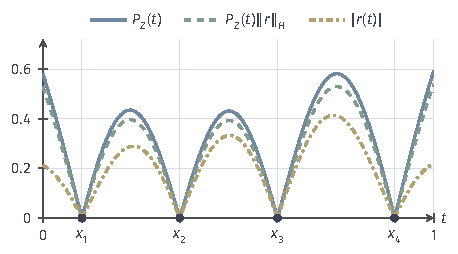
\includegraphics[width=77.5mm]{figures/02-abstract-mathematics/03-function-spaces/tikz/c5-power-function/figure.pdf}
  \caption{高斯核（$\sigma=0.15$）、观测点$x_i=0.1,0.35,0.6,0.9$的核插值幂函数$P_Z(t)=\|K_t-PK_t\|_H$（实线），以及图~\ref{fig:rkhs-observation-residual}中余项的绝对值$|r(t)|$（点划线）与上界$P_Z(t)\|r\|_H$（虚线，$\|r\|_H=0.911$）。幂函数在观测点处为零，只依赖于核与观测位置；余项总在上界之下。}
  \label{fig:rkhs-power-function}
\end{figure}

\paragraph{观测子空间自身的再生核}

前面处理的是一个给定函数的投影。换一个角度，观测子空间$M_Z$连同$H$的内积本身也是一个RKHS：对$g\in M_Z$，$g(x)=\langle g,K_x\rangle=\langle g,PK_x\rangle$，所以它的核截面是$PK_x$，再生核为
\begin{equation}
K_Z(x,z)=\langle PK_z,PK_x\rangle_H=\bm k_Z(x)^{\top}\bm G^{\dagger}\bm k_Z(z).
\label{eq:rkhs-projected-kernel}
\end{equation}
第二个等号用了$PK_x=\sum_jc_j(x)K_{x_j}$、$\bm c(x)=\bm G^{\dagger}\bm k_Z(x)$，以及式~\eqref{eq:rkhs-gram-calculus}和$\bm G^{\dagger}\bm G\bm G^{\dagger}=\bm G^{\dagger}$。同理，余下的$K-K_Z$是$M_Z^\perp$的再生核，因而也半正定，它的对角值就是$P_Z(x)^2$。

式~\eqref{eq:rkhs-projected-kernel}可以写成有限特征的内积。设$\bm G=\bm U\bm\Lambda\bm U^{\top}$是谱分解，$r$个正特征值组成$\bm\Lambda_r$，相应的特征向量组成$\bm U_r$。令
\[
\Phi_Z(x)=\bm\Lambda_r^{-1/2}\bm U_r^{\top}\bm k_Z(x)\in\mathbb R^r ,
\]
则$\Phi_Z(x)^{\top}\Phi_Z(z)=\bm k_Z(x)^{\top}\bm U_r\bm\Lambda_r^{-1}\bm U_r^{\top}\bm k_Z(z)=K_Z(x,z)$。$\Phi_Z$的第$k$个分量是函数$e_k=\lambda_k^{-1/2}\sum_j\bm U_{j,k}K_{x_j}$在$x$处的值，这些$e_k$构成$M_Z$的标准正交基：由式~\eqref{eq:rkhs-gram-calculus}，$\langle e_k,e_l\rangle=\lambda_k^{-1/2}\lambda_l^{-1/2}\bm u_k^{\top}\bm G\bm u_l=\delta_{k,l}$。

这里要分清两种近似。$Pf$近似的是一个给定的函数，误差取决于该函数的余项；$K_Z$近似的是核本身，它同时为$M_Z$中的所有函数提供再生关系，误差$K-K_Z$不涉及任何目标函数。式~\eqref{eq:rkhs-power-bound}把两者联系起来：给定函数的逐点误差不超过核误差的对角平方根乘以该函数的余项范数。中心应当怎样选取、读数带有噪声时采用什么拟合目标与惩罚、所得问题的解是否存在，都需要另外加入目标与观测模型；以核矩阵为工具的正则化回归可参考\BookChapterRef{chap:regression}{卷七《模型：经典模型》“回归”章中的核岭回归}，按样本抽取中心的低秩近似可参考\BookChapterRef{chap:dimensionality-reduction}{卷七“降维”章中的Nyström近似}。

% 第5章第4节：核的谱表示与有限特征（核积分算子与Mercer展开、核范数与谱系数、有限谱特征）。

\section{核的谱表示与有限特征}
\label{sec:rkhs-spectral}

到目前为止，核空间的全部结构都只由核决定，没有用到测度。本节固定核后再在输入集上加入一个测度，用核作积分核得到积分算子，从而把第~\ref{chap:operator-spectra-equations}章的紧自伴谱理论用到核上。要回答三个问题：积分算子的特征函数能否组成核本身的逐点展开；核范数在这些正交坐标下是什么形式；只保留前几个谱方向时，被控制的是核的误差还是某个给定函数的误差。

全节使用下面的条件：$X$是紧度量空间，$K$是$X\times X$上连续的半正定核，$\mu$是$X$上的有限正Borel测度，且具有\term{全支撑}（full support），即$X$的每个非空开集测度为正。记$M^2=\max_{x\in X}K(x,x)$。

\subsection{核积分算子与Mercer展开}
\label{sec:rkhs-mercer}
\label{subsubsec:compact-spectrum-mercer}

\paragraph{核积分算子}

在上述条件下定义\term{核积分算子}（kernel integral operator）
\[
(T_Kf)(x)=\int_XK(x,z)f(z)\,\mathrm d\mu(z),\qquad f\in L^2(\mu).
\]
$K$连续且$X$紧，所以$K$有界，又$\mu$有限，于是$K\in L^2(\mu\otimes\mu)$。由第~\ref{sec:ose-hilbert-schmidt}节，$T_K$是$L^2(\mu)$上的紧算子；由$K$对称及第~\ref{sec:ose-kernel-symmetry}节，$T_K$自伴。第~\ref{sec:ose-kernels}节已经强调，核公式只有连同测度才确定一个算子；这里的测度正是在核之外新加入的结构。

$T_K$的像比$L^2$等价类好得多：对任意$g\in L^2(\mu)$，$T_Kg$是处处有定义的连续函数。事实上，由Cauchy--Schwarz不等式，
\[
\begin{aligned}
|(T_Kg)(x)-(T_Kg)(x')|
&\le\Bigl(\int_X|K(x,z)-K(x',z)|^2\,\mathrm d\mu(z)\Bigr)^{1/2}\|g\|_{L^2}\\
&\le\mu(X)^{1/2}\sup_{z\in X}|K(x,z)-K(x',z)|\,\|g\|_{L^2},
\end{aligned}
\]
而$K$在紧集$X\times X$上一致连续，右端随$x'\to x$趋于零。

\paragraph{积分算子的正性}

第~\ref{sec:ose-kernel-symmetry}节指出，核的对称性只给出自伴，不给出$\langle T_Kf,f\rangle\ge0$。这里的正性来自核的半正定性，但两者的联系需要一个逼近论证：半正定性只涉及有限点组，积分则是连续的累计。

\begin{lemma}[半正定连续核给出正算子]
\label{lem:rkhs-positive-operator}
在本节条件下，对一切$f\in L^2(\mu)$，$\langle T_Kf,f\rangle_{L^2}=\iint K(x,z)f(x)f(z)\,\mathrm d\mu(x)\,\mathrm d\mu(z)\ge0$。
\end{lemma}

\begin{proof}
先设$f$连续。给定$\varepsilon>0$，函数$(x,z)\mapsto K(x,z)f(x)f(z)$在紧集上一致连续，取$\delta>0$使两点距离小于$\delta$时它的变化小于$\varepsilon$。用有限个半径$\delta/2$的开球覆盖$X$，再把它们依次去掉重叠部分，得到$X$的有限Borel划分$A_1,\ldots,A_N$，每块直径小于$\delta$；在每块中任取一点$x_i$。在$A_i\times A_j$上用$K(x_i,x_j)f(x_i)f(x_j)$代替被积函数，误差不超过$\varepsilon$，所以
\[
\Bigl|\langle T_Kf,f\rangle-\sum_{i,j}K(x_i,x_j)c_ic_j\Bigr|\le\varepsilon\,\mu(X)^2,\qquad c_i=f(x_i)\mu(A_i).
\]
中间的和是点组$x_1,\ldots,x_N$上Gram矩阵的二次型，非负；令$\varepsilon\to0$即得$\langle T_Kf,f\rangle\ge0$。对一般的$f\in L^2(\mu)$，连续函数在$L^2(\mu)$中稠密（第~\ref{sec:fs-density-separability}节），而$f\mapsto\langle T_Kf,f\rangle$在$L^2$中连续，非负性保持到极限。
\end{proof}

\paragraph{特征函数的连续代表}

于是$T_K$是$L^2(\mu)$上的紧、自伴、正算子，第~\ref{sec:ose-spectral-theorem}节的谱定理给出：非零特征值都是正数，至多可数，按重数重复排列为$\lambda_1\ge\lambda_2\ge\cdots>0$，只能在零处聚集；相应的特征函数$\psi_j$构成$(\ker T_K)^\perp$的标准正交基。

特征函数起初只是$L^2$等价类。若$T_K\psi=\lambda\psi$且$\lambda>0$，则$\psi=\lambda^{-1}T_K\psi$几乎处处成立，右端是连续函数，所以$\psi$有连续代表，以下总取这个代表。全支撑保证这个代表唯一：两个连续函数若几乎处处相等，使它们不相等的点组成开集，测度为零，由全支撑只能是空集。若$\mu$没有全支撑，例如$X=[0,1]$而$\mu$只是$[0,1/2]$上的Lebesgue测度，那么在$[1/2,1]$上任意改动的函数仍是同一个$L^2$元素，$L^2$坐标就无法确定函数在测度支撑之外的取值。

\paragraph{Mercer定理}

谱定理给出的是算子作用的展开$T_Kf=\sum_j\lambda_j\langle f,\psi_j\rangle\psi_j$，它在$L^2$范数下成立。对核本身，我们希望得到逐点甚至一致的展开，这正是\term{Mercer定理}（Mercer theorem）的内容\scite{mercer1909functions}。

\begin{theorem}[Mercer定理]
\label{thm:rkhs-mercer}
设$X$是紧度量空间，$K$是$X\times X$上连续的半正定核，$\mu$是$X$上全支撑的有限正Borel测度。设$\lambda_j>0$与连续的$\psi_j$是$T_K$的正特征值与$L^2(\mu)$标准正交特征函数。则
\begin{equation}
K(x,z)=\sum_j\lambda_j\psi_j(x)\psi_j(z)\qquad(x,z\in X),
\label{eq:rkhs-mercer}
\end{equation}
级数在$X\times X$上绝对且一致收敛；并且$\sum_j\lambda_j=\int_XK(x,x)\,\mathrm d\mu(x)<\infty$。
\end{theorem}

\begin{proof}[补充阅读：证明思路]
第一步，对角线上的部分和有界。令
\[
K^{(m)}(x,z)=K(x,z)-\sum_{j\le m}\lambda_j\psi_j(x)\psi_j(z),
\]
它连续。由谱展开，它对应的积分算子$T^{(m)}$满足
\[
\langle T^{(m)}f,f\rangle=\sum_{j>m}\lambda_j\langle f,\psi_j\rangle^2\ge0 .
\]若$K^{(m)}(x_0,x_0)<0$，由连续性存在$x_0$的开邻域$U$使$K^{(m)}<0$在$U\times U$上成立，取$f=\mathbf 1_U$，全支撑给出$\mu(U)>0$，于是$\langle T^{(m)}f,f\rangle<0$，矛盾。所以$\sum_{j\le m}\lambda_j\psi_j(x)^2\le K(x,x)\le M^2$对一切$m$与$x$成立。

第二步，固定$x$识别极限。由Cauchy--Schwarz不等式与第一步，
\[
\sum_{j=p}^q\lambda_j|\psi_j(x)\psi_j(z)|\le\Bigl(\sum_{j=p}^q\lambda_j\psi_j(x)^2\Bigr)^{1/2}M ,
\]
而第一步说明右端括号中的级数收敛，所以对固定的$x$，级数$S(x,z)=\sum_j\lambda_j\psi_j(x)\psi_j(z)$关于$z$一致收敛，$S(x,\cdot)$连续。另一方面，$\langle K(x,\cdot),\psi_j\rangle_{L^2}=(T_K\psi_j)(x)=\lambda_j\psi_j(x)$，所以连续函数$h=K(x,\cdot)-S(x,\cdot)$与每个$\psi_j$正交，属于$\ker T_K$；由于$T_Kh$连续且几乎处处为零，它处处为零，特别地$\int K(x,z)h(z)\,\mathrm d\mu(z)=0$。又$\int S(x,z)h(z)\,\mathrm d\mu(z)=\sum_j\lambda_j\psi_j(x)\langle\psi_j,h\rangle=0$，两式相减得$\int h^2\,\mathrm d\mu=0$。由全支撑与连续性，$h\equiv0$，即$K(x,z)=S(x,z)$。

第三步，一致收敛。在对角线上，连续函数$R_m(x)=K(x,x)-\sum_{j\le m}\lambda_j\psi_j(x)^2$随$m$单调下降并逐点趋于零。对任意$\varepsilon>0$，闭集$\{R_m\ge\varepsilon\}$随$m$递减且交为空集，由$X$的紧性，其中某一个已是空集，所以$R_m\to0$一致成立（这就是Dini定理）。再由第二步的Cauchy--Schwarz估计，$\sum_{j>m}\lambda_j|\psi_j(x)\psi_j(z)|\le\sqrt{R_m(x)R_m(z)}\le\max R_m$，得到$X\times X$上的绝对一致收敛。最后对对角线逐项积分（一致收敛且$\mu$有限），$\int K(x,x)\,\mathrm d\mu=\sum_j\lambda_j\int\psi_j^2\,\mathrm d\mu=\sum_j\lambda_j$。
\end{proof}

正特征值之和有限，说明$T_K$是\term{迹类算子}（trace-class operator）。比较两种展开：一般的紧自伴谱定理只说算子作用在$L^2$范数下展开，展开中的特征函数只是等价类；Mercer定理在核的连续性、半正定性与测度全支撑的条件下，给出核本身的逐点、一致展开，其中每个$\psi_j$都取连续代表。零特征值方向不出现在展开~\eqref{eq:rkhs-mercer}中；任何形如“除以$\lambda_j$”的公式，都只能在正谱方向上使用。

\paragraph{仿射核的谱}

第~\ref{sec:ose-kernels}节在$X=[-1,1]$、$\mathrm d\mu(z)=\mathrm dz/2$下计算过仿射核$K(x,z)=1+xz$的积分算子：$T_K1=1$，$T_Kx=x/3$，与$1,x$都正交的函数被消去。于是正特征值为$\lambda_1=1$、$\lambda_2=1/3$，标准正交特征函数为$\psi_1=1$、$\psi_2=\sqrt3\,x$（$\int3x^2\,\mathrm d\mu=1$）。Mercer展开只有两项：
\[
\lambda_1\psi_1(x)\psi_1(z)+\lambda_2\psi_2(x)\psi_2(z)=1+\tfrac13\cdot3xz=1+xz ,
\]
迹为$1+\tfrac13=\int_{-1}^1(1+x^2)\,\tfrac{\mathrm dx}2=\tfrac43$。零空间是$L^2(\mu)$中与$1,x$正交的全部函数，例如$x^2-1/3$。它是无限维的，却不出现在核的展开中。

\paragraph{最小值核的谱}

最小值核给出无穷多个正特征值，而且可以精确算出。在$[0,1]$上取Lebesgue测度，
\[
(T_K\psi)(x)=\int_0^xz\psi(z)\,\mathrm dz+x\int_x^1\psi(z)\,\mathrm dz .
\]
对连续的$\psi$，右端可微两次：$(T_K\psi)'(x)=\int_x^1\psi(z)\,\mathrm dz$，$(T_K\psi)''=-\psi$；并且$(T_K\psi)(0)=0$、$(T_K\psi)'(1)=0$。所以$T_K\psi=\lambda\psi$（$\lambda>0$）等价于边值问题$\lambda\psi''=-\psi$、$\psi(0)=0$、$\psi'(1)=0$，其解为$\psi(x)=\sin(\omega x)$，$\omega=\lambda^{-1/2}$且$\cos\omega=0$。归一化后
\[
\lambda_j=\frac1{\omega_j^2},\qquad \psi_j(x)=\sqrt2\,\sin(\omega_jx),\qquad \omega_j=\Bigl(j-\frac12\Bigr)\pi,\quad j=1,2,\ldots
\]
同样的推导说明$T_K\psi=0$迫使$\psi=-(T_K\psi)''=0$，所以零空间是平凡的，这些$\psi_j$构成$L^2(0,1)$的标准正交基。迹的检验：$\sum_j\lambda_j=\sum_j\frac{4}{(2j-1)^2\pi^2}=\frac12=\int_0^1x\,\mathrm dx$。

图~\ref{fig:rkhs-mercer-spectrum}画出前三个特征函数，并比较三种核的特征值衰减。最小值核的特征值按$j^{-2}$衰减；$\sigma=0.5$的高斯核在$[-1,1]$、$\mathrm dz/2$下的特征值衰减得快得多，第$12$个已降到$5\times10^{-9}$量级（数值求积所得）；仿射核只有两个正特征值。核越光滑，积分算子越强烈地压低高频方向，这里只作观察，不作为一般定理使用。

\begin{figure}[!htb]
  \centering
  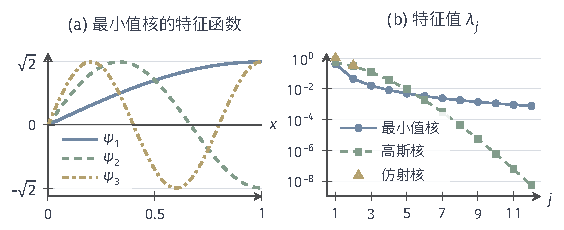
\includegraphics[width=95.5mm]{figures/02-abstract-mathematics/03-function-spaces/tikz/c5-mercer-spectrum/figure.pdf}
  \caption{Mercer特征函数与特征值衰减。(a)~最小值核在$[0,1]$、Lebesgue测度下的前三个特征函数$\psi_j=\sqrt2\sin((j-\frac12)\pi x)$，它们在$0$处为零、在$1$处导数为零；(b)~特征值（对数纵轴）：最小值核$\lambda_j=((j-\frac12)\pi)^{-2}$；高斯核（$\sigma=0.5$，$[-1,1]$，$\mathrm dz/2$）的特征值由40点Gauss--Legendre求积离散计算；仿射核只有$1$与$1/3$两个正特征值。}
  \label{fig:rkhs-mercer-spectrum}
\end{figure}

\subsection{核范数与谱系数}
\label{sec:rkhs-spectral-norm}

Mercer展开把核写成了特征映射$\Phi(x)=(\sqrt{\lambda_j}\psi_j(x))_j$的内积，这正好可以代入第~\ref{sec:rkhs-feature-maps}节的定理，读出核范数在谱坐标下的形式。

\paragraph{谱坐标下的核范数}

\begin{theorem}[核范数的谱表示]
\label{thm:rkhs-spectral-norm}
在定理~\ref{thm:rkhs-mercer}的条件下：
\begin{enumerate}
\item $\{\sqrt{\lambda_j}\,\psi_j\}$是$H_K$的标准正交基；
\item 函数$f:X\to\mathbb R$属于$H_K$，当且仅当存在实数列$(b_j)$满足$\sum_jb_j^2/\lambda_j<\infty$，且$f(x)=\sum_jb_j\psi_j(x)$对一切$x$成立。此时级数在$X$上绝对一致收敛，$b_j=\langle f,\psi_j\rangle_{L^2(\mu)}$，并且
\begin{equation}
\|f\|_{L^2(\mu)}^2=\sum_jb_j^2,\qquad \|f\|_{H_K}^2=\sum_j\frac{b_j^2}{\lambda_j}.
\label{eq:rkhs-two-norms}
\end{equation}
\end{enumerate}
\end{theorem}

\begin{proof}
令$\mathcal F=\ell^2$，$\Phi(x)=(\sqrt{\lambda_j}\psi_j(x))_j$。由定理~\ref{thm:rkhs-mercer}的第一步，$\|\Phi(x)\|^2=K(x,x)<\infty$；由Mercer展开，$\langle\Phi(x),\Phi(z)\rangle=K(x,z)$，所以$\Phi$是$K$的特征映射。先证可见子空间是整个$\ell^2$。设$w\in\ell^2$与每个$\Phi(x)$正交，即$\sum_jw_j\sqrt{\lambda_j}\psi_j(x)=0$对一切$x$成立。由于$\sqrt{\lambda_j}\le\sqrt{\lambda_1}$，系数$w_j\sqrt{\lambda_j}$平方可和，同一级数在$L^2(\mu)$中也收敛，其$L^2$极限与逐点极限几乎处处一致，因而为零；由$\psi_j$的标准正交性，$w_j\sqrt{\lambda_j}=0$，即$w=0$。

于是由定理~\ref{thm:rkhs-feature-space}，$w\mapsto f_w=\sum_jw_j\sqrt{\lambda_j}\psi_j$是从$\ell^2$到$H_K$的等距同构，单位向量$e_j$映为$\sqrt{\lambda_j}\psi_j$，这证明第1条。令$b_j=w_j\sqrt{\lambda_j}$，条件$w\in\ell^2$就是$\sum_jb_j^2/\lambda_j<\infty$，且$\|f_w\|_{H_K}^2=\sum_jw_j^2=\sum_jb_j^2/\lambda_j$。一致收敛来自
\[
\Bigl|\sum_{j>m}b_j\psi_j(x)\Bigr|\le\Bigl(\sum_{j>m}\frac{b_j^2}{\lambda_j}\Bigr)^{1/2}\Bigl(\sum_{j>m}\lambda_j\psi_j(x)^2\Bigr)^{1/2}\le M\Bigl(\sum_{j>m}\frac{b_j^2}{\lambda_j}\Bigr)^{1/2} .
\]
一致收敛的级数也在$L^2(\mu)$中收敛到同一函数，由标准正交性得$b_j=\langle f,\psi_j\rangle_{L^2}$与$\|f\|_{L^2}^2=\sum_jb_j^2$。
\end{proof}

\paragraph{两种范数的权重}

式~\eqref{eq:rkhs-two-norms}说明，同一组谱坐标$b_j$在两种范数中得到不同的权重：$L^2$范数对每个坐标一视同仁，核范数则把第$j$个坐标的平方放大$1/\lambda_j$倍。$L^2$中的单位方向$\psi_j$在$H_K$中的长度是$\lambda_j^{-1/2}$，$H_K$中真正的单位方向是$\sqrt{\lambda_j}\psi_j$。由于$\lambda_j\to0$，特征值小的方向在核范数中代价很高。

图~\ref{fig:rkhs-norm-weights}用最小值核说明这种差别。$f=\psi_1$与$g=\psi_1+0.1\psi_8$的图像几乎重合，$\|f-g\|_{L^2}=0.1$；但$\|f-g\|_{H_{\min}}=0.1\,\omega_8=0.1\times7.5\pi\approx2.36$，比$\|f\|_{H_{\min}}=\omega_1=\pi/2\approx1.57$还大。积分误差小并不意味着核范数误差小，核范数还计入了函数的振荡：对最小值核，$\|f\|_{H_{\min}}=\|f'\|_{L^2}$，$g$的高频小波纹带来很大的导数。

\begin{figure}[!htb]
  \centering
  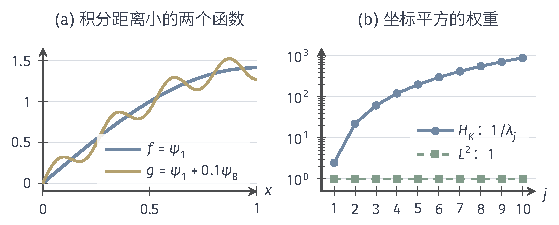
\includegraphics[width=94.6mm]{figures/02-abstract-mathematics/03-function-spaces/tikz/c5-norm-weights/figure.pdf}
  \caption{最小值核下两种范数的谱权重。(a)~$f=\psi_1$与$g=\psi_1+0.1\psi_8$，$\psi_j=\sqrt2\sin((j-\frac12)\pi x)$；两者的$L^2$距离为$0.1$，核范数距离却约为$2.36$。(b)~谱坐标平方在两种范数中的权重：$L^2$中恒为$1$，$H_K$中为$1/\lambda_j=((j-\frac12)\pi)^2$（对数纵轴），随$j$平方增长。}
  \label{fig:rkhs-norm-weights}
\end{figure}

\paragraph{哪些函数不在核空间中}

定理~\ref{thm:rkhs-spectral-norm}给出了$H_K$成员的两项要求：作为$L^2$元素，函数没有零谱分量；其谱坐标的加权平方和有限。两项要求可以分别不满足。在仿射核的例子中，$x^2=\tfrac13\psi_1+(x^2-\tfrac13)$含有零谱分量$x^2-\tfrac13$，所以不在$H_{\mathrm{aff}}$中，这一点也可以直接从$H_{\mathrm{aff}}$只含仿射函数看出。在最小值核的例子中零空间平凡，但常数函数$1$的谱坐标为$b_j=\int_0^1\sqrt2\sin(\omega_jx)\,\mathrm dx=\sqrt2/\omega_j$，于是$\sum_jb_j^2=\sum_j2/\omega_j^2=1=\|1\|_{L^2}^2$有限，而$\sum_jb_j^2/\lambda_j=\sum_j2$发散。常数$1$的谱展开在$L^2$中收敛，它却不属于$H_{\min}$，这与$H_{\min}$要求$f(0)=0$相符。

\paragraph{谱截断的两种尾和}

固定$f\in H_K$及其谱坐标$b_j$，令$f_m=\sum_{j\le m}b_j\psi_j$。由式~\eqref{eq:rkhs-two-norms}，
\begin{equation}
\|f-f_m\|_{L^2(\mu)}^2=\sum_{j>m}b_j^2\le\lambda_{m+1}\sum_{j>m}\frac{b_j^2}{\lambda_j}=\lambda_{m+1}\|f-f_m\|_{H_K}^2 ,
\label{eq:rkhs-tail-comparison}
\end{equation}
不等号用了$j>m$时$\lambda_j\le\lambda_{m+1}$。核范数尾和随$m\to\infty$趋于零，再由点值估计，
\[
|f(x)-f_m(x)|\le\sqrt{K(x,x)}\,\|f-f_m\|_{H_K}\le M\|f-f_m\|_{H_K},
\]
所以截断还一致收敛到$f$。逐点与一致控制来自核空间的点值有界性；一般的$L^2$正交展开没有这样的保证。式~\eqref{eq:rkhs-tail-comparison}还说明，对核范数不超过$R$的函数，$L^2$截断误差不超过$\sqrt{\lambda_{m+1}}R$，特征值衰减越快，这个统一的界越小。

以$H_{\min}$中的$f(x)=4x(1-x)$为例。它的谱坐标可以由分部积分算出：$b_j=4\sqrt2\bigl(2\omega_j^{-3}-(-1)^{j+1}\omega_j^{-2}\bigr)$，前三项约为$0.626,0.363,-0.068$；又$\|f\|_{L^2}^2=8/15$，$\|f\|_{H_{\min}}^2=\|f'\|_{L^2}^2=16/3$。取$m=3$，用总和减去前三项得$\|f-f_3\|_{L^2}\approx0.068$，$\|f-f_3\|_{H_{\min}}\approx1.07$。可以核对式~\eqref{eq:rkhs-tail-comparison}：$0.068^2\approx0.0046\le\lambda_4\times1.07^2\approx0.0083\times1.15\approx0.0095$。核范数尾和远大于$L^2$尾和，是因为$f'(1)=-4\ne0$而每个$\psi_j'(1)=0$，谱坐标只按$\omega_j^{-2}$衰减。

\paragraph{固定核而改变测度}

谱坐标依赖于测度，核范数却不依赖。仍取仿射核，把$[-1,1]$上的测度从$\mathrm dz/2$换成$\mathrm dz$，积分算子变为原来的两倍，特征值变为$2$与$2/3$，标准正交特征函数变为$1/\sqrt2$与$\sqrt{3/2}\,x$。对$f=a+bx$，新的谱坐标为$b_1=\sqrt2\,a$，$b_2=\int_{-1}^1(a+bx)\sqrt{3/2}\,x\,\mathrm dx=\sqrt{2/3}\,b$，于是
\[
\frac{b_1^2}{\lambda_1}+\frac{b_2^2}{\lambda_2}=\frac{2a^2}{2}+\frac{2b^2/3}{2/3}=a^2+b^2 ,
\]
与原来的核范数相同；而$L^2$范数平方从$a^2+b^2/3$变成了$2a^2+2b^2/3$。图~\ref{fig:rkhs-affine-norm-balls}在系数平面上画出三个单位球：核范数的单位球是圆，两个$L^2$单位球是形状不同的椭圆。这在一般情况下也成立：由定理~\ref{thm:rkhs-moore-aronszajn}，$H_K$的内积只由核决定；测度提供的是新的正交坐标和积分意义下的误差度量。

\begin{figure}[!htb]
  \centering
  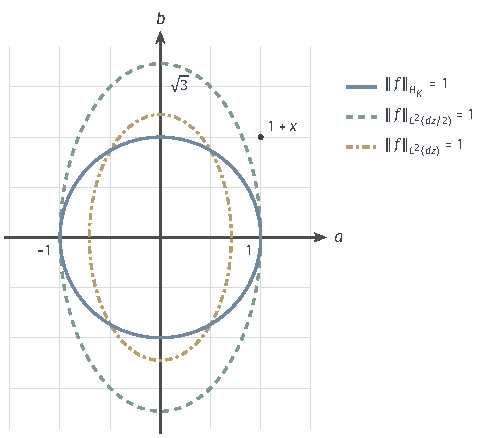
\includegraphics[width=82.4mm]{figures/02-abstract-mathematics/03-function-spaces/tikz/c5-affine-norm-balls/figure.pdf}
  \caption{仿射核$1+xz$在$[-1,1]$上，系数平面$(a,b)$（$f=a+bx$）中的三个单位球。实线圆是核范数单位球$a^2+b^2=1$，与测度无关；虚线椭圆是$L^2(\mathrm dz/2)$单位球$a^2+b^2/3=1$；点划线椭圆是$L^2(\mathrm dz)$单位球$2a^2+2b^2/3=1$。点$1+x$的核范数平方为$2$，$L^2(\mathrm dz/2)$范数平方为$4/3$。}
  \label{fig:rkhs-affine-norm-balls}
\end{figure}

\subsection{有限谱特征}
\label{sec:rkhs-finite-features}

上一小节截断的是一个给定函数的谱展开。本小节截断核本身，得到对所有函数同时适用的有限维表示，再与第~\ref{sec:rkhs-center-projection}节由观测中心得到的有限表示作比较。

\paragraph{谱特征与核近似}

保留前$m$个正谱方向，令
\[
\begin{aligned}
\Phi_m(x)&=\bigl(\sqrt{\lambda_1}\psi_1(x),\ldots,\sqrt{\lambda_m}\psi_m(x)\bigr)\in\mathbb R^m,\\
K_m(x,z)&=\Phi_m(x)^{\top}\Phi_m(z)=\sum_{j\le m}\lambda_j\psi_j(x)\psi_j(z).
\end{aligned}
\]
由定理~\ref{thm:rkhs-spectral-norm}，$K_m$是子空间$H_m=\operatorname{span}\{\psi_1,\ldots,\psi_m\}$（带$H_K$的内积）的再生核，$K-K_m$是其正交补的再生核。记对角余项$R_m(x)=K(x,x)-K_m(x,x)=\sum_{j>m}\lambda_j\psi_j(x)^2\ge0$，由Cauchy--Schwarz不等式，
\begin{equation}
|K(x,z)-K_m(x,z)|\le\sqrt{R_m(x)R_m(z)},\qquad
\int_XR_m\,\mathrm d\mu=\sum_{j>m}\lambda_j .
\label{eq:rkhs-kernel-truncation}
\end{equation}
Mercer定理保证$\max_xR_m(x)\to0$，所以$K_m$在$X\times X$上一致逼近$K$；积分意义下的误差恰好是特征值的尾和。对最小值核取$m=3$，$\int_0^1R_3\,\mathrm dx=\tfrac12-\sum_{j\le3}\omega_j^{-2}\approx0.0335$，$\max R_3\approx0.067$。

\paragraph{核误差与函数误差}

核误差与函数误差是两个不同的量。$f-f_m$属于$H_m$的正交补，而它的再生核是$K-K_m$，所以
\begin{equation}
|f(x)-f_m(x)|=\bigl|\langle f-f_m,(K-K_m)_x\rangle_{H_K}\bigr|\le\sqrt{R_m(x)}\,\|f-f_m\|_{H_K}.
\label{eq:rkhs-spectral-pointwise}
\end{equation}
右端的第一个因子只依赖于核与测度，第二个因子取决于$f$的谱坐标尾和。核误差小说明所有函数在单位核范数意义下被同时控制；某个具体函数的误差还取决于它的高频坐标有多大。另外，$f_m$既是$f$在$H_m$上的$L^2(\mu)$正交投影，也是$H_K$正交投影，因为$\psi_j$在两种内积下都两两正交。

\paragraph{谱截断与中心投影}

式~\eqref{eq:rkhs-spectral-pointwise}与第~\ref{sec:rkhs-center-projection}节的式~\eqref{eq:rkhs-power-bound}有完全相同的结构：一个$m$维子空间，它的再生核把余项的对角值留给误差界。两者的区别在于子空间由什么信息决定。中心投影的$M_Z$由观测位置决定，不需要测度，只需核值与读数；谱截断的$H_m$由测度下积分算子的特征函数决定，需要先求解积分算子的特征问题。

图~\ref{fig:rkhs-truncation-comparison}在最小值核上比较两者，都取三维：谱截断取$m=3$，中心投影取$Z=\{1/3,2/3,1\}$（第~\ref{sec:rkhs-center-projection}节已算出它是折线插值）。对核本身，中心投影的对角余项$P_Z^2$在中心处为零，但积分为$1/18\approx0.056$、最大值$1/12\approx0.083$，都大于谱截断的$0.0335$与$0.067$。对目标$f=4x(1-x)$，谱截断的$L^2$误差约$0.068$，小于中心投影的$0.081$；但中心投影的核范数误差约$0.77$、最大逐点误差约$0.11$，分别小于谱截断的$1.07$与$0.28$。谱截断在$x=1$附近误差最大，因为所有$\psi_j$在那里导数为零，而中心投影在$1$处恰好有一个观测。哪一种更好，取决于所用的误差度量，两种有限表示保留的是不同的子空间。

\begin{figure}[!htb]
  \centering
  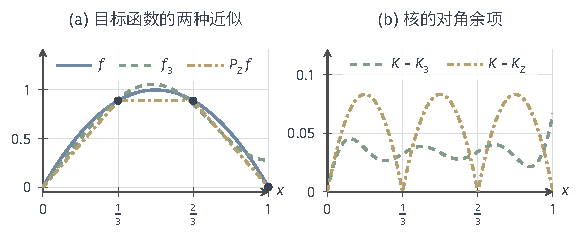
\includegraphics[width=98.2mm]{figures/02-abstract-mathematics/03-function-spaces/tikz/c5-truncation-comparison/figure.pdf}
  \caption{最小值核（$[0,1]$，Lebesgue测度）下三维谱截断与三个中心$Z=\{1/3,2/3,1\}$的投影。(a)~目标$f=4x(1-x)$（实线）、谱截断$f_3$（虚线）与中心投影$P_Zf$（点划线，即过黑点的折线）；(b)~核的对角余项$R_3(x)=K(x,x)-K_3(x,x)$与$P_Z(x)^2=K(x,x)-K_Z(x,x)$，后者在中心处为零但积分更大。}
  \label{fig:rkhs-truncation-comparison}
\end{figure}

在实际计算中，测度常常未知或只能通过样本给出，积分算子的特征函数也无法精确求得。由样本点构造核矩阵并取其谱分解，得到的正是第~\ref{sec:rkhs-center-projection}节的投影核$K_Z$及其有限特征$\Phi_Z$，而不是这里的$K_m$。样本中心与积分谱之间的关系、随机抽取中心或随机特征时的误差，需要另外引入抽样模型来分析；本节的尾和结论不能自动搬到这些数值方法上。

% 第5章第5节：本章小结。

\section{本章小结}
\label{sec:rkhs-summary}

本章从“有限个点值能否作为关于函数的可靠信息”出发，研究点值读取连续的Hilbert函数空间。核与空间之间有双向的对应：空间中每个点的读取有界时，Riesz表示把它写成与核截面$K_x$的内积，核$K(x,z)=\langle K_z,K_x\rangle$对称且半正定；反过来，任何半正定核都唯一地确定一个以它为再生核的空间$H_K$，构造经过系数组合、商去零长度方向、完备化和点值表示四步，核截面的有限组合在其中按核范数稠密。特征映射和核运算把“验证半正定”变成可以操作的检查：写成某个特征向量的内积，或由已知核经非负组合、乘积、换输入、缩放和极限得到。

几项看似相近的性质由不同的条件控制，不能互相代替。固定位置的点值有界由$K(x,x)$给出，全域统一控制要求核的对角有界；读数随位置连续要求核截面距离$\|K_x-K_z\|$随位置趋于零，离散空间$\ell^2(X)$说明前者不蕴含后者。有限观测下，Gram矩阵的零空间只表示系数的冗余，同一函数可以有多种写法；读数相同而函数不同，则来自观测子空间的正交补，它在无限维空间中总存在。投影的唯一性不等于系数的唯一性，最小范数插值由投影几何保证，与系数怎样选取无关。

加入测度后，紧度量空间上的连续半正定核产生紧、自伴、正的积分算子，Mercer定理把核本身展开为一致收敛的谱级数，特征函数在测度全支撑时有唯一的连续代表。核范数在谱坐标下按$1/\lambda_j$加权，于是积分误差小不等于核范数误差小，零谱分量或发散的加权和都把函数排除在$H_K$之外。改变测度会改变特征值和$L^2$坐标，核所定义的内积不变。截断核与截断给定函数控制的是不同的量：前者的误差只依赖核与测度，后者还取决于目标的谱尾；按积分谱截断与按观测中心投影保留的子空间由不同的信息决定，在不同的误差度量下各有优劣。

下一章利用这些空间与表示讨论具体的逼近问题：核截面的有限和能否逼近核空间之外的连续函数，以及怎样用有限个代表统一覆盖整类函数。由核矩阵出发的正则化拟合需要另外给定目标与惩罚，按样本抽取中心的数值近似需要抽样模型，用核比较概率分布则需要把概率测度嵌入核空间；这些问题分别属于优化与模型、统计推断和概率分布的研究，用核比较分布的方法可参考\BookChapterRef{chap:information-theory-and-statistical-geometry}{卷四《数学准备：流形、概率分布与统计推断》“概率分布的分析与优化”章中的最大均值差异}。


\chapter{函数与函数类的逼近}
\label{chap:function-approximation}

计算机只能存储有限个数。要在计算中使用$[0,1]$上的折线$f_*(x)=|x-1/2|$，可以记下多项式的系数、样条在结点处的值，或者一个小网络的权重；它们都用有限个数描述一个近似函数。由此产生三个问题。第一，固定目标、定义域和误差范数后，哪些有限表示能把误差压到任意小，误差又怎样随次数、结点数或单元数下降？第二，目标有多个变量时，表示所需的数目怎样随维数增长，能否利用变量之间的分离结构减少数目？第三，若事先只知道目标属于某个函数类，例如全体以$1$为Lipschitz常数、绝对值不超过$1$的函数，能否预先备好有限个代表，使类中每个成员都靠近其中之一，又至少需要多少个代表？

前三个问题依次改变了被逼近的对象。第~\ref{sec:apx-single-function}节固定一个目标，比较多项式、样条、核截面和神经单元四种生成方式；它们的预算可以随精度增加，结论分为“能否任意逼近”和“误差下降多快”两类，后者总要额外的光滑性。第~\ref{sec:apx-multivariate}节固定变量的分组方式，研究由单变量函数组成多变量函数的张量积空间，以及只用少数乘积项的低秩表示。第~\ref{sec:apx-function-classes}节把对象从单个函数换成整个函数类，量词随之改变：每个成员各有一个近似，不等于一套共同的有限代表适用于全体。为此先用Arzelà--Ascoli判据刻画一致距离下的相对紧性，再用覆盖数计量所需代表的个数。

本章使用第~\ref{chap:function-spaces}章的一致范数、$L^2$空间、正交基与投影，第~\ref{chap:rkhs}章的点值界与核截面，以及第~\ref{chap:metric-spaces}章的全有界与紧致性。逼近在这里是表示能力的问题：根据数据确定系数、用优化算法训练参数以及统计误差保证，都需要另加目标函数或随机数据，留给后续相应部分。

% 第8章第1节：给定函数的有限逼近（多项式、样条、核截面、神经网络）。

\section{给定函数的有限逼近}
\label{sec:apx-single-function}

本节固定一个目标函数、它的定义域和衡量误差的范数，再挑选一类生成单元，用它们的有限线性组合去接近目标。主要的误差范数是一致范数$\|f\|_\infty=\sup_x|f(x)|$（第~\ref{sec:fs-uniform-norm}节），它要求整个定义域上的误差同时变小。四小节分别使用多项式、分段直线、固定宽度的高斯核截面和神经单元；每一种都有自己的预算，即次数、结点数、中心个数或单元个数。

贯穿全节的目标是
\[
  f_*(x)=\left|x-\frac12\right|,\qquad x\in[0,1].
\]
它连续，却在$x=1/2$处有折点。后面会看到：多项式只能随次数增加而逼近它，含结点$1/2$的线性样条和两个ReLU单元却能精确表示它。这个对照比较的是同一目标在不同生成规则下需要的条件，不能由一个例子推出某种方案对所有目标都更节省。

读结论时要分清两类陈述。“对每个$\varepsilon>0$，存在某个预算下的近似，误差小于$\varepsilon$”是可变预算下的存在性，预算可以随$\varepsilon$增长；“预算为$m$时误差不超过某个量”是固定预算下的误差保证，通常要求目标满足额外的光滑性。前者回答能否逼近，后者回答逼近得多快。

\subsection{多项式逼近}
\label{sec:apx-polynomial}

多项式是最早被系统研究的逼近工具：给定次数，它由有限个系数确定，求值只需加法和乘法。本小节先构造一列具体的多项式并证明它一致逼近任意连续目标，再把构造中真正用到的性质提炼成一般定理。

\paragraph{连续模}

要估计全区间上的误差，需要一个量来记录目标在小尺度上能变化多少。

\begin{definition}[连续模]
\label{def:apx-modulus-of-continuity}
设$f$是区间$I$上的有界函数。对$\delta>0$，令
\[
  \omega_f(\delta)=\sup\bigl\{|f(s)-f(t)|:\ s,t\in I,\ |s-t|\le\delta\bigr\},
\]
称$\omega_f$为$f$的\term{连续模}（modulus of continuity）。
\end{definition}

连续模关于$\delta$单调不减。$f$在$I$上一致连续，恰好等价于$\omega_f(\delta)\to0$（$\delta\downarrow0$）；在紧区间上，连续函数都一致连续（定理~\ref{thm:metric-compact-uniform}），所以$C([0,1])$中每个函数的连续模都趋于零。若$f$满足$|f(s)-f(t)|\le L|s-t|$，则$\omega_f(\delta)\le L\delta$。

对贯穿目标，$|f_*(s)-f_*(t)|\le|s-t|$；取$s=0$、$t=\delta$（$\delta\le1/2$）时等号成立，而$f_*$的取值在$[0,1/2]$中，因此
\[
  \omega_{f_*}(\delta)=\min\{\delta,1/2\}.
\]
再看$g(x)=\sqrt x$：由$|\sqrt s-\sqrt t|\le\sqrt{|s-t|}$且在$s=0$处取等号，得$\omega_g(\delta)=\sqrt\delta$（$\delta\le1$）。两个函数都连续，但$g$在原点附近变化得更剧烈，连续模下降得更慢。后面的误差界都以连续模表示，这个差别会直接反映在速率上。

\paragraph{Bernstein多项式}

现在构造逼近多项式。固定整数$m\ge1$，在等距结点$j/m$处读取$f$的值，令
\begin{equation}
  B_mf(x)=\sum_{j=0}^{m}f\Bigl(\frac jm\Bigr)w_{m,j}(x),
  \qquad
  w_{m,j}(x)=\binom mj x^j(1-x)^{m-j},
  \label{eq:apx-bernstein}
\end{equation}
称为$f$的$m$次\term{Bernstein多项式}（Bernstein polynomial）\scite{bernstein1912demonstration}。每个权重$w_{m,j}$都是次数为$m$的多项式，所以$B_mf$是次数至多$m$的多项式；系数只需要$m+1$个结点值。

权重有两个直接可见的性质。在$[0,1]$上每个$w_{m,j}(x)\ge0$；由二项式定理，
\[
  \sum_{j=0}^m w_{m,j}(x)=\bigl(x+(1-x)\bigr)^m=1.
\]
因此$B_mf(x)$是结点值的凸组合，取值不会超出结点值的范围。图~\ref{fig:apx-bernstein-approx}画出$f_*$的三个Bernstein多项式：曲线随$m$增大而贴近折线，最大误差都出现在折点处。

\begin{figure}[!htb]
  \centering
  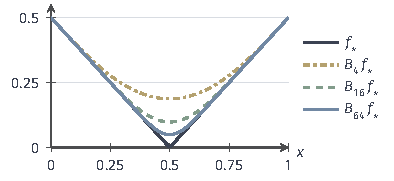
\includegraphics[width=66.7mm]{figures/02-abstract-mathematics/03-function-spaces/tikz/c6-bernstein-approx/figure.pdf}
  \caption{折线$f_*(x)=|x-1/2|$（黑）及其Bernstein多项式$B_4f_*$、$B_{16}f_*$、$B_{64}f_*$。每条曲线都是结点值的凸组合，位于$f_*$上方；一致误差都在$x=1/2$处取得，依次为$0.1875$、$0.0982$、$0.0497$，次数每增至四倍，误差约减半。}
  \label{fig:apx-bernstein-approx}
\end{figure}

凸组合只说明取值范围，还没有说明权重集中在哪些结点上。若权重主要落在离$x$较近的结点，$B_mf(x)$就主要由$f$在$x$附近的值决定。下面的矩恒等式把这个直觉写成精确的计算。

\begin{lemma}[Bernstein权重的矩]
\label{lem:apx-bernstein-moments}
对$0\le x\le1$和$m\ge1$，
\[
  \sum_{j=0}^m j\,w_{m,j}(x)=mx,\qquad
  \sum_{j=0}^m j(j-1)\,w_{m,j}(x)=m(m-1)x^2,
\]
从而
\begin{equation}
  \sum_{j=0}^m\Bigl(\frac jm-x\Bigr)^2w_{m,j}(x)=\frac{x(1-x)}m\le\frac1{4m}.
  \label{eq:apx-bernstein-variance}
\end{equation}
\end{lemma}

\begin{proof}
第一式利用$j\binom mj=m\binom{m-1}{j-1}$。$j=0$的项为零，把下标改为$k=j-1$，
\[
  \sum_{j=0}^m j\,w_{m,j}(x)
  =mx\sum_{k=0}^{m-1}\binom{m-1}{k}x^k(1-x)^{m-1-k}=mx,
\]
最后一步再次使用二项式定理。第二式同理利用$j(j-1)\binom mj=m(m-1)\binom{m-2}{j-2}$，把下标改为$k=j-2$即得；$m=1$时两边都为零。

对中心矩，把$(j/m-x)^2$展开，并用$j^2=j(j-1)+j$：
\[
  \sum_{j}\Bigl(\frac jm-x\Bigr)^2w_{m,j}
  =\frac{m(m-1)x^2+mx}{m^2}-2x\cdot\frac{mx}{m}+x^2
  =\frac{x(1-x)}m .
\]
最后由$x(1-x)\le1/4$得到上界$1/(4m)$。
\end{proof}

式~\eqref{eq:apx-bernstein-variance}说明，以$w_{m,j}(x)$为权重时，结点$j/m$与$x$的平均平方距离只有$x(1-x)/m$。若读者熟悉概率，这些权重正是二项分布$\mathrm{Bin}(m,x)$的概率，上述三式分别是总概率、均值与方差；证明只用到有限和，不依赖概率论。

\paragraph{近邻与远处的误差分解}

有了权重的集中性，就可以把误差分成两部分来控制：近邻结点上$f$的值接近$f(x)$，远处结点的总权重很小。

\begin{theorem}[Bernstein--Weierstrass逼近]
\label{thm:apx-bernstein}
设$f\in C([0,1])$。对每个$m\ge1$和每个$\delta>0$，
\begin{equation}
  \|B_mf-f\|_\infty\le\omega_f(\delta)+\frac{\|f\|_\infty}{2m\delta^2}.
  \label{eq:apx-bernstein-error}
\end{equation}
因此$\|B_mf-f\|_\infty\to0$（$m\to\infty$）。特别地，$[0,1]$上的多项式在$C([0,1])$中一致稠密。
\end{theorem}

\begin{proof}
固定$x\in[0,1]$。由权重和为一，误差可以写成
\[
  B_mf(x)-f(x)=\sum_{j=0}^m\Bigl[f\Bigl(\frac jm\Bigr)-f(x)\Bigr]w_{m,j}(x).
\]
按$|j/m-x|\le\delta$与$|j/m-x|>\delta$把结点分成近邻与远处两组。

近邻组中每个差值的绝对值不超过$\omega_f(\delta)$，而近邻权重之和不超过$1$，所以这一组的贡献至多为$\omega_f(\delta)$。

远处组中每个差值不超过$2\|f\|_\infty$。对远处的结点有$1<(j/m-x)^2/\delta^2$，于是由式~\eqref{eq:apx-bernstein-variance}，
\[
  \sum_{|j/m-x|>\delta}w_{m,j}(x)
  \le\frac1{\delta^2}\sum_{j=0}^m\Bigl(\frac jm-x\Bigr)^2w_{m,j}(x)
  \le\frac1{4m\delta^2},
\]
这一组的贡献至多为$2\|f\|_\infty/(4m\delta^2)$。两组相加后右端不依赖$x$，对$x$取上确界即得式~\eqref{eq:apx-bernstein-error}。

为了得到收敛，次序很重要。任给$\varepsilon>0$，先利用一致连续性选$\delta$使$\omega_f(\delta)<\varepsilon/2$；保持这个$\delta$不变，再取$m$足够大，使$\|f\|_\infty/(2m\delta^2)<\varepsilon/2$。若先固定$m$再缩小$\delta$，第二项会变大，论证不能成立。
\end{proof}

图~\ref{fig:apx-bernstein-weights}以$m=50$、$x=0.3$、$\delta=0.15$为例画出全部权重。蓝色的近邻结点占去权重$0.980$，黄色的远处结点只有$0.020$；矩估计给出的远处权重上界为$x(1-x)/(m\delta^2)=0.187$，再放大为$1/(4m\delta^2)=0.222$。上界相当保守，但它不依赖$x$，这正是全区间共用的误差界所需要的。

\begin{figure}[!htb]
  \centering
  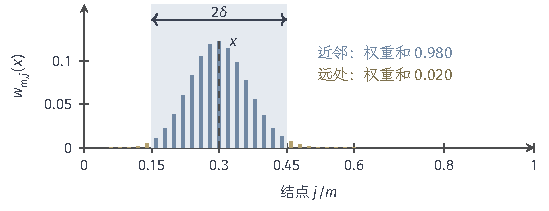
\includegraphics[width=93.0mm]{figures/02-abstract-mathematics/03-function-spaces/tikz/c6-bernstein-weights/figure.pdf}
  \caption{Bernstein权重的集中性：$m=50$、$x=0.3$时各结点$j/m$上的权重$w_{m,j}(x)$。蓝底为近邻窗口$|j/m-x|\le\delta=0.15$，窗口内权重和为$0.980$，窗口外（黄色）仅$0.020$。误差分解中，近邻部分由连续模$\omega_f(\delta)$控制，远处部分由二阶中心矩$x(1-x)/m$控制。}
  \label{fig:apx-bernstein-weights}
\end{figure}

\paragraph{折点目标与收敛速度}

定理~\ref{thm:apx-bernstein}保证$f_*$可以被多项式任意逼近，但任何一个多项式都不等于$f_*$：多项式处处可微，而$f_*$在$1/2$处的左右导数分别为$-1$和$1$。“可以任意逼近”与“能被某个有限次多项式精确表示”是两回事。

收敛有多快取决于目标的正则性。若$f$是$L$-Lipschitz的，可以不经过近远分解，直接用Cauchy--Schwarz不等式估计：
\[
  |B_mf(x)-f(x)|
  \le L\sum_{j}\Bigl|\frac jm-x\Bigr|w_{m,j}(x)
  \le L\Bigl(\sum_j\Bigl(\frac jm-x\Bigr)^2w_{m,j}(x)\Bigr)^{1/2}
  \le\frac{L}{2\sqrt m}.
\]
对$f_*$，$L=1$，这个界在$m=4,16,64$时分别为$0.25$、$0.125$、$0.0625$，实际误差$0.1875$、$0.0982$、$0.0497$与它同阶。对$\sqrt x$只有$|f(s)-f(t)|\le|s-t|^{1/2}$，同样的论证（先对$|j/m-x|^{1/2}$用Cauchy--Schwarz）只给出$(4m)^{-1/4}$。条件越弱，这个构造能保证的速率越慢。

Bernstein多项式也不是相应次数下最好的多项式。由引理~\ref{lem:apx-bernstein-moments}，
\[
  B_m(x^2)=\frac{m(m-1)x^2+mx}{m^2}=x^2+\frac{x(1-x)}m,
\]
所以对$x^2$本身，误差恰为$1/(4m)$，而$x^2$只是一个二次多项式。这个构造的价值在于每一步都可以验证，并给出所有连续函数共同的收敛机制；最佳逼近的误差需要另外研究。

\paragraph{Stone--Weierstrass定理}

回看定理~\ref{thm:apx-bernstein}的结论：$[0,1]$上的多项式在一致范数下稠密。把多项式换成其他函数族、把区间换成其他紧集时，哪些性质仍然是关键？多项式族对加法、数乘和乘法封闭，含有常数，而且函数$x$能区分任意两个不同的点。下面的定理说明这几条已经足够。

设$K$是非空紧度量空间，$C(K)$为$K$上全体实值连续函数，配备一致范数。若子空间$\mathcal A\subseteq C(K)$对逐点乘法封闭，就称它是\term{子代数}（subalgebra）；若对任意$x\ne y$都有$h\in\mathcal A$使$h(x)\ne h(y)$，就称$\mathcal A$\term{分离点}（separates points）。

\begin{theorem}[Stone--Weierstrass定理]
\label{thm:apx-stone-weierstrass}
设$K$是非空紧度量空间，$\mathcal A\subseteq C(K)$是含有常数函数且分离点的子代数，则$\mathcal A$在$C(K)$中按一致范数稠密：对每个$f\in C(K)$和$\varepsilon>0$，存在$h\in\mathcal A$使$\|f-h\|_\infty<\varepsilon$。
\end{theorem}

这一结论由Stone对Weierstrass多项式逼近定理的推广给出\scite{stone1948generalized}。它立即覆盖多变量的情形：在紧集$K\subset\mathbb R^d$上，$d$元多项式组成含常数的子代数，坐标函数分离点，因此多元多项式在$C(K)$中稠密。另一个例子是单位圆周：把$[0,2\pi]$的两端看成同一点，三角多项式$\sum_{k=0}^n(a_k\cos kt+b_k\sin kt)$对乘法封闭（由积化和差），含有常数，$\cos t$与$\sin t$合起来分离圆周上的点，因此在圆周上的连续函数中稠密。

两个条件各自不可缺少。在$[-1,1]$上，偶多项式组成含常数的子代数，但对每个偶多项式都有$p(x)=p(-x)$，它不能分离$x$与$-x$；一致极限仍是偶函数，因此奇函数$x$不在闭包中。在$[0,1]$上，满足$p(0)=0$的多项式组成分离点的子代数，但不含常数；一致极限都在$0$处取零，所以常函数$1$不在闭包中。

\begin{proof}[补充阅读：证明思路]
记$\overline{\mathcal A}$为一致闭包，它仍是含常数的子代数。第一步，若$h\in\overline{\mathcal A}$，则$|h|\in\overline{\mathcal A}$：在$[-\|h\|_\infty,\|h\|_\infty]$上用多项式$p$一致逼近$|t|$（定理~\ref{thm:apx-bernstein}经线性变量代换），$p\circ h$属于$\overline{\mathcal A}$且一致接近$|h|$。由$\max\{g,h\}=(g+h+|g-h|)/2$和$\min\{g,h\}=(g+h-|g-h|)/2$，$\overline{\mathcal A}$对有限个函数取最大、最小封闭。第二步，由分离点和常数，对任意$x\ne y$和实数$a,b$，存在$h\in\mathcal A$满足$h(x)=a$、$h(y)=b$：取$u$使$u(x)\ne u(y)$，令$h=a+(b-a)(u-u(x))/(u(y)-u(x))$。第三步，固定$f$、$\varepsilon$和$x$，对每个$y$取$h_y$使$h_y(x)=f(x)$、$h_y(y)=f(y)$；集合$\{z:h_y(z)<f(z)+\varepsilon\}$是开集并覆盖$K$，由紧性取有限个，令$g_x=\min h_{y_i}$，则$g_x<f+\varepsilon$且$g_x(x)=f(x)$。再对开集$\{z:g_x(z)>f(z)-\varepsilon\}$用一次紧性，取有限个$g_{x_k}$的最大值，即得$\overline{\mathcal A}$中与$f$一致误差小于$\varepsilon$的函数。
\end{proof}

\paragraph{稠密性与误差速率}

Stone--Weierstrass定理只回答“能否任意逼近”，不提供任何速率：它没有说明达到精度$\varepsilon$需要多少项，证明中的紧性步骤也不给出项数。定理~\ref{thm:apx-bernstein}之所以能给出速率，是因为对目标另加了连续模或Lipschitz常数等定量条件。要比较不同生成单元的效率，必须先固定这样一个函数类；第~\ref{sec:apx-function-classes}节将把“固定一个函数类”本身作为研究对象。

\subsection{样条逼近}
\label{sec:apx-splines}

多项式是全局的：改变一个系数，整个区间上的函数值都会改变，Bernstein权重也在整个$(0,1)$上非零。另一种思路是把区间切成小段，每段只用低次多项式，段与段之间按一定光滑性衔接。这类分段多项式称为\term{样条}（spline），分段的位置称为\term{结点}（knot）。本小节从最简单的连续分段直线开始。

\paragraph{线性插值与连续模界}

固定结点$0=t_0<t_1<\cdots<t_N=1$，记最大间距$h=\max_i(t_{i+1}-t_i)$。对$x\in[t_i,t_{i+1}]$，令
\begin{equation}
  S_hf(x)=(1-s)f(t_i)+s\,f(t_{i+1}),\qquad s=\frac{x-t_i}{t_{i+1}-t_i}\in[0,1].
  \label{eq:apx-linear-interpolant}
\end{equation}
相邻两段在公共结点取同一个值，所以$S_hf$是经过全部结点值的连续折线，称为$f$的线性插值。全体在每段上为一次函数的连续函数组成\term{线性样条}（linear spline）空间，它是$N+1$维的线性空间；$S_h$则是从结点值产生其中一个元素的操作。图~\ref{fig:apx-spline-hat}(a)画出一个光滑函数在七个等距结点上的线性插值。

\begin{theorem}[线性插值的误差]
\label{thm:apx-linear-interpolation}
在上述记号下，若$f\in C([0,1])$，则
\begin{equation}
  \|f-S_hf\|_\infty\le\omega_f(h).
  \label{eq:apx-spline-modulus}
\end{equation}
若进一步$f\in C^2([0,1])$，则
\begin{equation}
  \|f-S_hf\|_\infty\le\frac{h^2}{8}\|f''\|_\infty .
  \label{eq:apx-spline-quadratic}
\end{equation}
\end{theorem}

\begin{proof}
先证连续模界。在单元$[t_i,t_{i+1}]$上，利用$(1-s)+s=1$，
\[
  f(x)-S_hf(x)=(1-s)\bigl(f(x)-f(t_i)\bigr)+s\bigl(f(x)-f(t_{i+1})\bigr).
\]
$x$到两个端点的距离都不超过$h$，所以两个差值都不超过$\omega_f(h)$，凸组合也不超过$\omega_f(h)$。对所有单元取上确界即得式~\eqref{eq:apx-spline-modulus}。

再证二阶界。固定单元和其中一点$x\in(t_i,t_{i+1})$，令$g=f-S_hf$，它在两端为零。取
\[
  \lambda=\frac{g(x)}{(x-t_i)(x-t_{i+1})},\qquad
  G(u)=g(u)-\lambda(u-t_i)(u-t_{i+1}),
\]
则$G$在$t_i$、$x$、$t_{i+1}$三点为零。两次使用Rolle定理，存在$\xi\in(t_i,t_{i+1})$使$G''(\xi)=0$。由于$S_hf$在单元内是一次函数，$G''(\xi)=f''(\xi)-2\lambda$，故$\lambda=f''(\xi)/2$，即
\[
  f(x)-S_hf(x)=\frac{f''(\xi)}2(x-t_i)(x-t_{i+1}).
\]
在单元上$|(x-t_i)(x-t_{i+1})|\le(t_{i+1}-t_i)^2/4\le h^2/4$，代入即得式~\eqref{eq:apx-spline-quadratic}。
\end{proof}

两个界依据不同。连续模界只用了凸组合，对任何连续目标成立，并且不要求结点等距：只要一列网格的最大间距$h\to0$，插值就一致收敛到$f$。二阶界多用了$f''$的有界性，换来$h^2$的速率；Rolle定理与插值余项可参考\BookChapterRef{chap:univariate-differentiation}{卷一“一元函数的微分”章}。

二阶界中的常数$1/8$不能改进。取$f(x)=x^2$，只用两个结点$0$和$1$，则$S_hf(x)=x$，误差$x-x^2$在$x=1/2$处取最大值$1/4$；此时$h=1$、$\|f''\|_\infty=2$，右端$h^2\|f''\|_\infty/8=1/4$，等号成立。

\paragraph{额外光滑性带来的速率}

二阶速率所用的光滑性不能省略。取等距结点$t_i=i/N$，$N$为奇数，此时$1/2$不是结点，而落在单元$[(N-1)/(2N),(N+1)/(2N)]$的中点。$f_*$在这个单元的两个端点取值都是$h/2$，插值在单元内恒为$h/2$，而$f_*(1/2)=0$；其余单元上$f_*$本身就是直线，插值没有误差。因此$\|f_*-S_hf_*\|_\infty=h/2$，只按一阶下降，这与$\omega_{f_*}(h)=h$的界同阶。

图~\ref{fig:apx-spline-rates}在对数坐标中比较两种目标。光滑函数$\sin(\pi x)$的实测误差几乎落在二阶界$\pi^2h^2/8$上，斜率为$2$；$f_*$的误差落在直线$h/2$上，斜率为$1$。网格宽度控制的是表示的分辨率，同一分辨率下能达到的精度取决于目标的光滑性。

\begin{figure}[!htb]
  \centering
  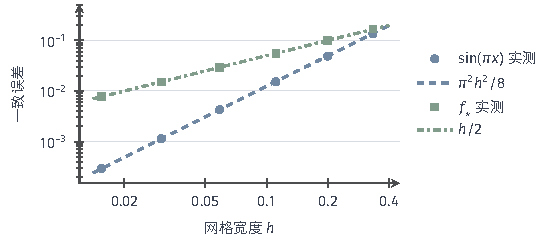
\includegraphics[width=93.4mm]{figures/02-abstract-mathematics/03-function-spaces/tikz/c6-spline-rates/figure.pdf}
  \caption{等距线性插值的一致误差与网格宽度$h=1/N$（$N=3,5,\ldots,65$为奇数，$1/2$不是结点），双对数坐标。光滑目标$\sin(\pi x)$的误差（圆点）贴近二阶界$\pi^2h^2/8$；折线$f_*$的误差（方块）恰为$h/2$，只按一阶下降。}
  \label{fig:apx-spline-rates}
\end{figure}

\paragraph{帽形基与局部修改}

线性插值可以改写成固定基函数的线性组合。对每个结点$t_i$，令$\varphi_i$为在$t_i$处取$1$、在其余结点处取$0$的线性样条；它在$[t_{i-1},t_{i+1}]$上呈三角形，在别处为零，称为\term{帽形函数}（hat function）。于是
\[
  S_hf=\sum_{i=0}^{N}f(t_i)\varphi_i,\qquad \sum_{i=0}^N\varphi_i\equiv1 .
\]
系数恰好是结点值，基函数非负且和为一，这正是式~\eqref{eq:apx-linear-interpolant}中凸组合的来源。

若结点包含$1/2$，例如取$t_0=0$、$t_1=1/2$、$t_2=1$，则$f_*$在每段上都是直线，
\[
  f_*=\tfrac12\varphi_0+0\cdot\varphi_1+\tfrac12\varphi_2 ,
\]
三个系数就精确表示了它。这比任何次数的多项式都节省，原因在于结点恰好放在折点上；同一组结点并不能精确表示任意连续目标。

帽形基的支撑只覆盖相邻两段，因此修改一个结点值只影响局部。图~\ref{fig:apx-spline-hat}(b)把$t_3=1/2$处的值由$0.5$改为$0.8$，插值只在$[t_2,t_4]=[1/3,2/3]$上改变。这里有两个不同来源的性质：局部性来自基函数的支撑，误差界来自凸组合；后面换用其他基时，需要分别重新检查。

\begin{figure}[!htb]
  \centering
  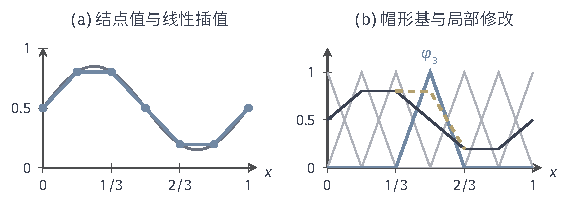
\includegraphics[width=96.2mm]{figures/02-abstract-mathematics/03-function-spaces/tikz/c6-spline-hat/figure.pdf}
  \caption{线性样条与帽形基，结点$t_i=i/6$。(a)~目标$0.5+0.35\sin(2\pi x)$（灰）及其线性插值（蓝折线），圆点为结点值。(b)~七个帽形函数（细灰），其中$\varphi_3$加粗；黑色折线为(a)中的插值，把$t_3$处的结点值改为$0.8$后得到黄色虚线，变化只发生在$\varphi_3$的支撑$[1/3,2/3]$上。}
  \label{fig:apx-spline-hat}
\end{figure}

\paragraph{高次样条与系数恢复}

把每段的一次函数换成$k$次多项式，并要求在内部结点处$k-1$阶导数连续，就得到$k$次样条。$N$段各有$k+1$个系数，每个内部结点施加$k$个衔接条件，空间维数为$(k+1)N-k(N-1)=N+k$。常用的三次样条维数为$N+3$，而结点值只提供$N+1$个条件，还需补充两个端点条件，插值才唯一。

更高的次数和衔接阶带来更光滑的近似，代价是系数与结点值不再直接对应。以等距结点上的三次B样条$\beta_3$为例（$\beta_3(0)=2/3$，$\beta_3(\pm1)=1/6$，在$|s|\ge2$处为零），若$S(x)=\sum_jc_j\beta_3(x-j)$，则在整数结点处
\[
  S(i)=\frac{c_{i-1}+4c_i+c_{i+1}}6 .
\]
要让$S$经过给定的结点值，必须先解这个线性方程组恢复系数；直接把结点值当系数，得到的是相邻值的加权平均。因此要分清三件事：样条空间是哪个候选集合，插值条件从中挑出哪个元素，系数又如何从样本求出。图像重采样中的插值核、预滤波和边界延拓属于信号处理的具体问题，可参考\BookChapterRef{chap:signal-analysis}{卷三“信号”章}。

\subsection{核截面逼近}
\label{sec:apx-kernel-sections}

第~\ref{chap:rkhs}章从半正定核$K$构造了再生核Hilbert空间$H_K$，并证明核截面$K_x=K(\cdot,x)$的有限线性组合在$H_K$中按核范数稠密（第~\ref{sec:rkhs-from-kernel}节）。本小节把核截面当作生成单元，问：在$H_K$之外，有限核和能否逼近更一般的连续目标？

\paragraph{核空间内与核空间外}

先说明核范数下的逼近在什么意义上已经是一致逼近。由再生关系$f(x)=\langle f,K_x\rangle_{H_K}$和Cauchy--Schwarz不等式，$|f(x)|\le\sqrt{K(x,x)}\,\|f\|_{H_K}$（第~\ref{sec:rkhs-kernel-properties}节）。若$\sup_xK(x,x)<\infty$，则$\|f\|_\infty\le\sup_x\sqrt{K(x,x)}\,\|f\|_{H_K}$，核范数下的逼近自动是一致逼近。

本小节固定$[0,1]$上宽度为$\sigma>0$的高斯核
\[
  K_\sigma(x,c)=\exp\Bigl(-\frac{(x-c)^2}{2\sigma^2}\Bigr),
\]
它满足$K_\sigma(x,x)=1$，所以$\|f\|_\infty\le\|f\|_{H_K}$。问题在于$f_*$不属于这个$H_K$。原因是$H_K$中的函数都可微。由再生关系，两个差商$(K_{x+t}-K_x)/t$与$(K_{x+t'}-K_x)/t'$的内积等于
\[
  \frac{K(x+t,x+t')-K(x+t,x)-K(x,x+t')+K(x,x)}{tt'},
\]
$K_\sigma$二阶连续可微，$t,t'\to0$时它趋于$\partial_1\partial_2K(x,x)$。于是差商之差的范数平方$\|(K_{x+t}-K_x)/t-(K_{x+t'}-K_x)/t'\|_{H_K}^2$趋于零，差商在完备空间$H_K$中收敛到某个$D_x$；于是对$f\in H_K$，
\[
  \frac{f(x+t)-f(x)}t=\Bigl\langle f,\frac{K_{x+t}-K_x}t\Bigr\rangle_{H_K}\to\langle f,D_x\rangle_{H_K},
\]
$f$在$x$处可导。$f_*$在$1/2$处不可导，所以$f_*\notin H_K$，第~\ref{chap:rkhs}章的稠密性结论不能直接用于它。

\paragraph{中心差分与加权多项式}

证明的思路是借助多项式。先固定中心$c_0=1/2$，令$w(x)=K_\sigma(x,c_0)$。对中心求导，$\partial_cK_\sigma(x,c)=(x-c)K_\sigma(x,c)/\sigma^2$，每求一次导就多出一个关于$x$的一次因子。由归纳法，
\begin{equation}
  \partial_c^jK_\sigma(x,c_0)=w(x)P_j(x),
  \label{eq:apx-gaussian-derivative}
\end{equation}
其中$P_j$是$j$次多项式，最高次项系数为$\sigma^{-2j}$。归纳步骤是：对$K_\sigma(x,c)Q(x-c)$再关于$c$求导，得到$K_\sigma(x,c)\bigl[(x-c)Q(x-c)/\sigma^2-Q'(x-c)\bigr]$，第一项把次数提高一次并把首项系数乘以$\sigma^{-2}$，第二项次数更低。

导数本身还不是有限核和，需要用差分代替。对固定的$j$和步长$t>0$，中心$j$阶前向差分
\begin{equation}
  D_t^{(j)}(x)=t^{-j}\sum_{\ell=0}^{j}(-1)^{j-\ell}\binom j\ell K_\sigma(x,c_0+\ell t)
  \label{eq:apx-center-difference}
\end{equation}
是$j+1$个核截面的线性组合。反复使用微积分基本定理，可以把它写成导数的平均：
\[
  D_t^{(j)}(x)=t^{-j}\int_0^t\!\!\cdots\!\int_0^t\partial_c^jK_\sigma(x,c_0+u_1+\cdots+u_j)\,\mathrm du_1\cdots\mathrm du_j .
\]
积分中的中心都落在$[c_0,c_0+jt]$内。$\partial_c^jK_\sigma$在紧矩形$[0,1]\times[c_0,c_0+1]$上一致连续，所以
\[
  \begin{aligned}
  \sup_{x\in[0,1]}\bigl|D_t^{(j)}(x)-w(x)P_j(x)\bigr|
  &\le\sup_{x\in[0,1],\ 0\le u\le jt}\bigl|\partial_c^jK_\sigma(x,c_0+u)-\partial_c^jK_\sigma(x,c_0)\bigr|\\
  &\to0\qquad(t\downarrow0).
  \end{aligned}
\]
一致性来自这里的二元一致连续，逐点求导本身只给出每个$x$处的收敛。图~\ref{fig:apx-gaussian-sections}(b)画出$j=1$的情形：$t=0.1$时差分与导数的一致偏差为$2.14$，$t=0.02$时降为$0.44$。

\paragraph{高斯核截面的一致稠密性}

有了每个$wP_j$都能由有限核和一致逼近，剩下的工作是把任意连续目标化成$w$乘一个多项式。

\begin{theorem}[固定宽度高斯核截面的一致稠密性]
\label{thm:apx-gaussian-dense}
固定$\sigma>0$。全体有限和$\sum_{\ell=1}^{M}a_\ell K_\sigma(\cdot,c_\ell)$（$M\in\mathbb N$、$a_\ell\in\mathbb R$、$c_\ell\in\mathbb R$均可随目标和精度变化）在$C([0,1])$中按一致范数稠密。
\end{theorem}

\begin{proof}
设$f\in C([0,1])$，$\varepsilon>0$。

第一步，把目标化成加权多项式。$w$在$[0,1]$上连续且有正下界，所以$f/w\in C([0,1])$。由定理~\ref{thm:apx-bernstein}，存在多项式$P$使$\|f/w-P\|_\infty<\varepsilon/2$；由$0<w\le1$，得$\|f-wP\|_\infty<\varepsilon/2$。

第二步，把$P$写成$P_0,\ldots,P_n$的组合，其中$n=\deg P$。$P_j$的首项系数$\sigma^{-2j}\ne0$，所以从$1,x,\ldots,x^n$到$P_0,\ldots,P_n$的系数矩阵是对角元非零的三角矩阵，可逆。因此$P=\sum_{j=0}^nb_jP_j$，$wP=\sum_jb_jwP_j$。

第三步，对每个$j$用差分代替$wP_j$。由上一段的一致收敛，可选步长$t_j$使$\|D_{t_j}^{(j)}-wP_j\|_\infty<\varepsilon/\bigl(2(n+1)(|b_j|+1)\bigr)$。于是$g=\sum_jb_jD_{t_j}^{(j)}$是有限个高斯核截面的线性组合，且
\[
  \|f-g\|_\infty\le\|f-wP\|_\infty+\sum_{j=0}^n|b_j|\,\|wP_j-D_{t_j}^{(j)}\|_\infty<\varepsilon.
\]
\end{proof}

图~\ref{fig:apx-gaussian-sections}(a)取$\sigma=0.15$，在$M$个等距中心处插值$f_*$：$M=5$时一致误差为$0.061$，$M=9$时为$0.024$。这只是一种具体的选系数方式，并不是定理证明中的构造。

\begin{figure}[!htb]
  \centering
  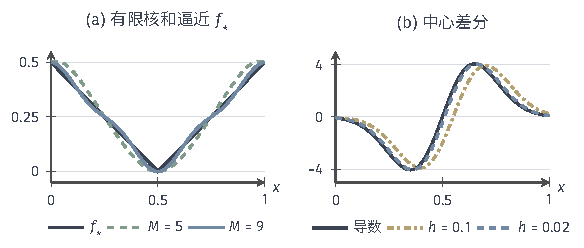
\includegraphics[width=98.9mm]{figures/02-abstract-mathematics/03-function-spaces/tikz/c6-gaussian-sections/figure.pdf}
  \caption{固定宽度$\sigma=0.15$的高斯核截面。(a)~在等距中心$c_\ell=(\ell-1)/(M-1)$处插值$f_*$的有限核和，$M=5$（虚线）与$M=9$（实线），一致误差分别为$0.061$与$0.024$。(b)~中心差分$(K_\sigma(x,\frac12+t)-K_\sigma(x,\frac12))/t$随$t$减小一致逼近导数$(x-\frac12)K_\sigma(x,\frac12)/\sigma^2$，这是一个加权一次多项式。}
  \label{fig:apx-gaussian-sections}
\end{figure}

\paragraph{两种稠密性与结论的条件}

现在可以区分两个命题。第~\ref{chap:rkhs}章的结论是：核截面的有限和在$H_K$中按核范数稠密，它只涉及$H_K$内部的函数。定理~\ref{thm:apx-gaussian-dense}则是：有限核和在$C([0,1])$中按一致范数稠密，它涉及$H_K$之外的目标，例如$f_*$。紧度量空间$X$上的连续核若使$H_K$在$C(X)$中稠密，就称为\term{通用核}（universal kernel）。由于$\|g\|_\infty\le\sup_x\sqrt{K(x,x)}\,\|g\|_{H_K}$，$H_K$中每个元素都能被有限核和一致逼近，所以“$H_K$在$C(X)$中稠密”与“有限核和在$C(X)$中稠密”是同一回事。Steinwart证明了高斯核在$\mathbb R^d$的任意紧子集上都是通用核\cite{steinwart2001kernel}；上面给出的是一维区间上的一条具体证明路线。

定理的条件同样需要逐条读清。

第一，中心、项数和系数都允许随目标与精度变化。若只允许一组预先固定的有限中心，得到的是$C([0,1])$中的有限维子空间；有限维子空间是闭的且不是全空间，不可能稠密。

第二，定理没有对系数或核范数设统一预算。第~\ref{sec:apx-arzela-ascoli}节将证明，核范数不超过$R$的函数组成$C([0,1])$中的紧集，因而是闭集；它只含$H_K$中的函数，所以不含$f_*$，$f_*$到它的一致距离为正。由此，逼近$f_*$的有限核和的核范数必然随精度趋于无穷。

第三，存在性证明不提供数值稳定的选系数方法。差分中出现因子$t^{-j}$，系数会随精度变大；朴素插值也有同样的问题：$\sigma=0.15$时，$M=13$个等距中心的插值误差为$0.023$，最大系数约为$415$；$M=17$时最大系数约为$1.06\times10^6$，误差反而升到$0.097$。如何在给定数据和惩罚下稳定地确定系数，属于后续优化与拟合问题。

\subsection{神经网络逼近}
\label{sec:apx-neural}

神经单元先对输入作仿射变换，再送入一个固定的一元函数，即激活函数；网络的输出是若干单元的线性组合。本小节从一维的分段线性构造开始，把它和样条联系起来，再陈述一般的通用逼近定理。

\paragraph{ReLU单元与折点目标}

\term{整流线性单元}（rectified linear unit，ReLU）使用激活函数$\rho(s)=\max\{s,0\}$。一个单元$x\mapsto a\rho(wx+b)$在$x=-b/w$处折一次，一侧为零，另一侧为斜率$aw$的直线。对贯穿目标，直接验证
\[
  f_*(x)=\rho\Bigl(x-\frac12\Bigr)+\rho\Bigl(\frac12-x\Bigr):
\]
当$x\ge1/2$时第一项为$x-1/2$、第二项为零；当$x\le1/2$时第一项为零、第二项为$1/2-x$。两个单元的输入权重符号相反，偏置都把折点放在$1/2$，输出直接相加，见图~\ref{fig:apx-relu-units}(a)。这个表示由两侧的计算验证，与训练过程无关。

\paragraph{线性样条的ReLU分解}

每个ReLU单元贡献一个折点，这提示连续折线都可以用ReLU单元写出。设连续函数$f$在$[t_0,t_N]$上以$t_0<t_1<\cdots<t_N$为结点分段线性，第$k$段$[t_k,t_{k+1}]$上的斜率为$s_k$。则
\begin{equation}
  f(x)=f(t_0)+s_0(x-t_0)+\sum_{k=1}^{N-1}(s_k-s_{k-1})\rho(x-t_k),\qquad x\in[t_0,t_N].
  \label{eq:apx-relu-spline}
\end{equation}
验证只需比较两侧：右端在$x=t_0$处等于$f(t_0)$，是连续折线；在第$k$段内部，$\rho(x-t_1),\ldots,\rho(x-t_k)$都已进入线性部分，斜率为$s_0+\sum_{i=1}^k(s_i-s_{i-1})=s_k$，与$f$相同。两个连续函数在起点相等且每段斜率相同，所以处处相等。每个单元只在自己的结点之后改变斜率，图~\ref{fig:apx-relu-units}(b)画出了逐项相加的部分和。

在$[0,1]$上$t_0=0$时，$s_0x=s_0\rho(x)$，常数项可以作为输出偏置，因此式~\eqref{eq:apx-relu-spline}恰是一个有$N$个隐藏单元的单隐藏层ReLU网络；在一般区间上可用$x=\rho(x)-\rho(-x)$补出线性项。结合定理~\ref{thm:apx-linear-interpolation}，取等距结点$t_k=k/N$并对$f\in C([0,1])$作线性插值，就得到一个$N$单元网络$g_N$，满足
\[
  \|f-g_N\|_\infty\le\omega_f(1/N).
\]
这是一维ReLU网络通用逼近的构造性证明，同时给出速率：对$L$-Lipschitz目标，误差不超过$L/N$。

\begin{figure}[!htb]
  \centering
  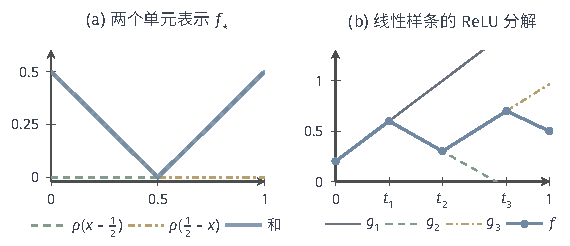
\includegraphics[width=96.6mm]{figures/02-abstract-mathematics/03-function-spaces/tikz/c6-relu-units/figure.pdf}
  \caption{ReLU单元的有限组合。(a)~$\rho(x-\frac12)$与$\rho(\frac12-x)$之和恰为$f_*$。(b)~结点$0,t_1,t_2,t_3,1=0,0.25,0.5,0.8,1$、结点值$0.2,0.6,0.3,0.7,0.5$的线性样条$f$（蓝），按式~\eqref{eq:apx-relu-spline}写成$0.2+1.6\rho(x)-2.8\rho(x-0.25)+\frac{38}{15}\rho(x-0.5)-\frac73\rho(x-0.8)$；细线$g_1,g_2,g_3$依次是前一、二、三个单元的部分和，每加一个单元就在对应结点处改变斜率。}
  \label{fig:apx-relu-units}
\end{figure}

\paragraph{单隐藏层通用逼近定理}

一维构造依赖分段线性的特殊结构。对多维输入和一般激活函数，需要下面的存在定理。

\begin{theorem}[单隐藏层网络的通用逼近]
\label{thm:apx-universal-approximation}
设$X\subset\mathbb R^d$是非空紧集，激活函数$\sigma:\mathbb R\to\mathbb R$连续且不是多项式。则形如
\begin{equation}
  g(\bm x)=\sum_{j=1}^{M}a_j\,\sigma(\bm w_j^{\top}\bm x+b_j),
  \qquad M\in\mathbb N,\ a_j,b_j\in\mathbb R,\ \bm w_j\in\mathbb R^d
  \label{eq:apx-one-hidden-layer}
\end{equation}
的函数全体在$C(X)$中按一致范数稠密。
\end{theorem}

这一形式的结论由Leshno、Lin、Pinkus与Schocken证明\cite{leshno1993approximation}，他们的结果对更广的局部有界、分段连续激活也成立；此前Cybenko对S型激活给出了同类结论\scite{cybenko1989approximation}。这里只陈述并使用连续激活的情形，证明从略。在式~\eqref{eq:apx-one-hidden-layer}外再加一个输出偏置，不改变结论。

定理的条件都可以用例子检查。Sigmoid函数$1/(1+e^{-s})$、$\tanh s$和ReLU都连续且不是多项式，所以都满足条件；定理不要求激活处处可微。

多项式激活必须排除。若$\sigma$是$r$次多项式，则$\sigma(\bm w^{\top}\bm x+b)$是$\bm x$的至多$r$次多项式，无论$M$多大，$g$都落在“$d$元至多$r$次多项式”这个有限维子空间中。若$X$含有内点，函数$x_1^{r+1}$不在这个子空间中；有限维子空间是闭的，所以$x_1^{r+1}$与它的一致距离为正。增加宽度不能增加可表达的次数，“使用了非线性函数”不能代替“非多项式”这一条件。

偏置也不能省略。在$[0,1]$上取ReLU且令所有$b_j=0$，则$\rho(w_jx)$在$w_j>0$时等于$w_jx$，在$w_j\le0$时恒为零，所有组合都形如$cx$。这样的函数在$0$处为零，无法逼近常函数$1$。

\paragraph{表示能力之外的问题}

通用逼近定理断言“存在”一组参数，它不回答以下几个问题，每个都需要单独的条件和论证。

参数不可识别。同一个函数有许多参数表示：交换隐藏单元的次序不改变输出；ReLU的正齐次性给出$a\rho(wx+b)=(a/\lambda)\rho(\lambda wx+\lambda b)$（$\lambda>0$）；在$[0,1]$上还有$f_*(x)=2\rho(x-\frac12)-\rho(x)+\frac12$，它与前面的两单元表示使用不同的单元。因此不能由函数反推出唯一的参数。

寻找参数与推广到新样本是另外的问题。定理不说明梯度方法能否找到逼近参数，也不说明由有限样本训练出的网络在新输入上误差小；相应的分析可参考\BookChapterRef{chap:feedforward-networks}{卷八“前馈神经网络”章}和\BookChapterRef{chap:deep-learning-theory}{卷六“深度学习的可学习性”章}。

评价范数也要说明。若输入服从$X$上的概率测度$\mu$，则$\|f-g\|_{L^2(\mu)}\le\|f-g\|_\infty$，一致逼近自动给出平均意义下的逼近；反方向不成立，一个只在小区域上很高的尖峰可以使$L^2(\mu)$误差很小而一致误差很大。向量值目标可以逐坐标逼近，再把各坐标的隐藏单元并列放进同一隐藏层。

% 第8章第2节：多变量函数的组合表示（张量积函数空间、低秩分离表示）。

\section{多变量函数的组合表示}
\label{sec:apx-multivariate}

上一节讨论的是选择什么生成单元。目标有多个变量时，还要决定怎样由单变量的函数组成多变量的函数。本节把变量分成两组$x$与$y$（每组本身也可以是向量），研究乘积$u(x)v(y)$的有限和。张量积空间描述全部这样的组合能张成什么；低秩表示则在这个空间中只使用少数几个乘积项。两者可以使用同样的单变量生成函数，区别在于用了多少个乘积方向。

记$(u\otimes v)(x,y)=u(x)v(y)$，称为$u$与$v$的乘积函数，也称为\term{张量积}（tensor product）。

\subsection{张量积函数空间}
\label{sec:apx-tensor-product}

\paragraph{乘积函数与系数矩阵}

固定$x$方向的函数$\varphi_1,\ldots,\varphi_m$和$y$方向的函数$\psi_1,\ldots,\psi_n$，并设每组都线性无关。所有乘积$\varphi_i\otimes\psi_k$的线性组合可以写成
\begin{equation}
  F(x,y)=\sum_{i=1}^m\sum_{k=1}^n c_{i,k}\varphi_i(x)\psi_k(y)=\bm\varphi(x)^{\top}\bm C\,\bm\psi(y),
  \label{eq:apx-coefficient-matrix}
\end{equation}
其中$\bm\varphi(x)=(\varphi_1(x),\ldots,\varphi_m(x))^{\top}$，$\bm\psi(y)$类似，$\bm C=[c_{i,k}]\in\mathbb R^{m\times n}$是系数矩阵。把$\bm C$按列拉直成$\operatorname{vec}(\bm C)\in\mathbb R^{mn}$，则$F(x,y)=(\bm\psi(y)\otimes\bm\varphi(x))^{\top}\operatorname{vec}(\bm C)$，这里的$\otimes$是Kronecker积；有限维的张量积与Kronecker积可参考\BookChapterRef{chap:linear-operations}{卷一“向量、矩阵与张量的运算”章}。

系数矩阵由$F$唯一确定。若$\sum_{i,k}c_{i,k}\varphi_i(x)\psi_k(y)\equiv0$，固定$y$后，由$\varphi_i$线性无关得$\sum_kc_{i,k}\psi_k(y)=0$对每个$i$和每个$y$成立，再由$\psi_k$线性无关得全部$c_{i,k}=0$。因此$mn$个乘积函数线性无关，组成的空间维数为$mn$。

矩阵的秩对应最少的乘积项数。若在这两个子空间中$F=\sum_{j=1}^ru_j\otimes v_j$，把$u_j=\bm\varphi^{\top}\bm a_j$、$v_j=\bm\psi^{\top}\bm b_j$代入，由系数唯一性得$\bm C=\sum_{j=1}^r\bm a_j\bm b_j^{\top}$，所以$r\ge\operatorname{rank}\bm C$；反之，$\bm C$的秩分解直接给出$\operatorname{rank}\bm C$项的表示。例如$F(x,y)=x+y=x\cdot1+1\cdot y$，在基$\{1,x\}$与$\{1,y\}$下系数矩阵为$\left[\begin{smallmatrix}0&1\\1&0\end{smallmatrix}\right]$，秩为$2$，所以$x+y$不是单个乘积函数；而$e^{x+y}=e^xe^y$只需一项。

\paragraph{乘积测度下的内积}

要讨论$L^2$误差，需要知道乘积函数的内积怎样计算。设$(X,\mu)$与$(Y,\nu)$是有限测度空间，$\mu\otimes\nu$为乘积测度。对实值$u,u'\in L^2(\mu)$与$v,v'\in L^2(\nu)$，由Cauchy--Schwarz不等式，$uu'\in L^1(\mu)$且$vv'\in L^1(\nu)$，于是$(u\otimes v)(u'\otimes v')$在$\mu\otimes\nu$下可积，由第~\ref{chap:measure-spaces}章中$\sigma$有限乘积测度的Fubini定理，
\begin{equation}
  \langle u\otimes v,u'\otimes v'\rangle_{L^2(\mu\otimes\nu)}
  =\int_X u u'\,\mathrm d\mu\int_Y v v'\,\mathrm d\nu
  =\langle u,u'\rangle_{L^2(\mu)}\langle v,v'\rangle_{L^2(\nu)} .
  \label{eq:apx-product-inner}
\end{equation}
特别地$\|u\otimes v\|=\|u\|\,\|v\|$，乘积函数属于$L^2(\mu\otimes\nu)$。乘积的内积分解为两个因子内积的乘积，这是下面构造正交基的依据。

\paragraph{正交基的乘积}

由式~\eqref{eq:apx-product-inner}，两组标准正交系的乘积仍是标准正交系。下面的定理说明，在可分情形它还是完备的。

\begin{theorem}[乘积正交基]
\label{thm:apx-product-basis}
设$(X,\mu)$与$(Y,\nu)$是有限测度空间，实空间$L^2(\mu)$与$L^2(\nu)$可分，分别有标准正交基$\{e_i\}_{i\ge1}$与$\{f_k\}_{k\ge1}$。则$\{e_i\otimes f_k\}_{i,k\ge1}$是$L^2(\mu\otimes\nu)$的标准正交基。
\end{theorem}

\begin{proof}
标准正交性由式~\eqref{eq:apx-product-inner}直接得到，只需证明完备：若$F\in L^2(\mu\otimes\nu)$与所有$e_i\otimes f_k$正交，则$F=0$。

由Tonelli定理，$\int_X\bigl(\int_Y|F(x,y)|^2\mathrm d\nu\bigr)\mathrm d\mu<\infty$，所以对$\mu$-几乎处处的$x$，截面$F(x,\cdot)\in L^2(\nu)$。对每个$k$令$G_k(x)=\int_YF(x,y)f_k(y)\,\mathrm d\nu(y)$。由Cauchy--Schwarz不等式$|G_k(x)|\le\|F(x,\cdot)\|_{L^2(\nu)}$，故$G_k\in L^2(\mu)$。

$F\cdot(e_i\otimes f_k)$是两个$L^2(\mu\otimes\nu)$元素之积，因而可积，Fubini定理允许先对$y$积分：
\[
  \langle G_k,e_i\rangle_{L^2(\mu)}=\int_X\!\int_YF(x,y)e_i(x)f_k(y)\,\mathrm d\nu\,\mathrm d\mu=\langle F,e_i\otimes f_k\rangle=0 .
\]
对所有$i$成立，所以$G_k=0$几乎处处。可数个零测集的并仍是零测集，因此存在$\mu$-零测集$N$，使$x\notin N$时对所有$k$都有$\langle F(x,\cdot),f_k\rangle=G_k(x)=0$，从而$F(x,\cdot)=0$于$L^2(\nu)$。最后$\|F\|^2=\int_X\|F(x,\cdot)\|^2\,\mathrm d\mu=0$。这里用到了$\{f_k\}$可数，即$L^2(\nu)$可分。
\end{proof}

定理说明乘积函数的有限和在$L^2(\mu\otimes\nu)$中稠密：任何$F$都可以按$\{e_i\otimes f_k\}$展开（第~\ref{sec:fs-orthonormal-bases}节），截断即得有限和。抽象地说，把$L^2(\mu)$与$L^2(\nu)$中元素乘积的有限和配上式~\eqref{eq:apx-product-inner}的内积，再完备化，得到\term{Hilbert张量积}（Hilbert tensor product）$L^2(\mu)\mathbin{\hat\otimes}L^2(\nu)$；上述定理表明它恰好可以实现为$L^2(\mu\otimes\nu)$。区间上的Lebesgue测度满足可分条件（第~\ref{sec:fs-density-separability}节）。

需要注意，空间中的一般元素不是单个乘积函数，甚至不是有限个乘积之和：它的系数是一个无限矩阵$[\langle F,e_i\otimes f_k\rangle]$，可能有无穷多个非零奇异值。下一小节将证明$e^{xy}$就是这样的例子。

\paragraph{张量积网格插值}

现在把一维线性插值推广到二维。在$[0,1]$上取等距结点$t_i=i/(m-1)$（$i=0,\ldots,m-1$），帽形函数为$\varphi_0,\ldots,\varphi_{m-1}$，网格宽度$h=1/(m-1)$。二维插值取
\[
  (\Pi f)(x,y)=\sum_{i=0}^{m-1}\sum_{k=0}^{m-1}f(t_i,t_k)\,\varphi_i(x)\varphi_k(y),
\]
系数是网格上的函数值，基函数是一维帽形函数的乘积。乘积$\varphi_i\otimes\varphi_k$的支撑是矩形$[t_{i-1},t_{i+1}]\times[t_{k-1},t_{k+1}]$，任一查询点只受它所在网格单元四个角点的影响，这就是双线性插值；它在每个单元内对$x$、$y$分别是一次的，但一般含有交叉项$xy$。图~\ref{fig:apx-tensor-grid}(a)画出$m=5$时一个乘积基的支撑和一个查询点所用的四个角点。

误差可以由一维结果逐个方向得到。记$I_x$为只对$x$作线性插值（$y$固定），$I_y$类似，则$\Pi=I_xI_y$。由于$I_x$是结点值的凸组合，$\|I_xg\|_\infty\le\|g\|_\infty$。若$f\in C^2([0,1]^2)$，利用定理~\ref{thm:apx-linear-interpolation}，
\[
  \|f-\Pi f\|_\infty\le\|f-I_xf\|_\infty+\|I_x(f-I_yf)\|_\infty
  \le\frac{h^2}{8}\bigl(\|\partial_x^2f\|_\infty+\|\partial_y^2f\|_\infty\bigr).
\]
同样的论证在$d$维给出误差至多$d\,h^2\max_i\|\partial_i^2f\|_\infty/8$，系数个数则为$m^d$。

\paragraph{组合规模与维数}

$m^d$的增长是张量积构造的直接代价。设每个$\|\partial_i^2f\|_\infty\le1$，要求误差不超过$\varepsilon=10^{-3}$，上式要求$h^2\le8\varepsilon/d$。$d=2$时$h\le0.0632$，取$m=17$，共$289$个系数；$d=6$时$h\le0.0365$，需要$m=29$，共$29^6\approx5.9\times10^8$个系数。每个方向的分辨率只略有提高，总数却增长了六个数量级。这种由完整组合造成的规模爆炸常称为\term{维数灾难}（curse of dimensionality），图~\ref{fig:apx-tensor-grid}(b)画出了$m=4$与$m=10$时$m^d$随$d$的增长。

\begin{figure}[!htb]
  \centering
  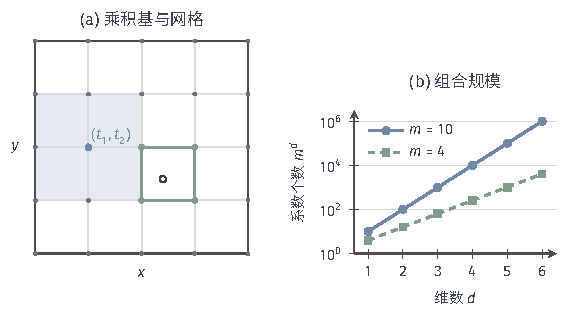
\includegraphics[width=95.0mm]{figures/02-abstract-mathematics/03-function-spaces/tikz/c6-tensor-grid/figure.pdf}
  \caption{张量积网格。(a)~每轴$m=5$个结点，蓝底为乘积帽形基$\varphi_1(x)\varphi_2(y)$的支撑，蓝点为其中心结点$(t_1,t_2)$；空心圆为一个查询点，双线性插值只用它所在单元的四个角点（绿）。(b)~完整张量积系数个数$m^d$随维数$d$指数增长（对数纵轴）。}
  \label{fig:apx-tensor-grid}
\end{figure}

乘积结构也出现在核方法中。第~\ref{sec:rkhs-kernel-operations}节说明两个核的乘积仍是核；$\mathbb R^d$上的高斯核正是$d$个一维高斯核的乘积，其核截面$K_{(x',y')}=K_{1,x'}\otimes K_{2,y'}$是一维核截面的张量积。插值核的频率性质、混叠和实际重建算法属于前面提到的信号问题，这里不展开。

\subsection{低秩分离表示}
\label{sec:apx-low-rank}

完整的张量积展开使用全部$mn$个系数。若系数矩阵近似低秩，就可以只用少数几个乘积项。本小节固定两组变量，研究
\[
  F_r(x,y)=\sum_{j=1}^r u_j(x)v_j(y)
\]
能以什么误差逼近给定的二元函数，其中$r$称为项数。

\paragraph{指数函数的Taylor分离}

以$E(x,y)=e^{xy}$、$(x,y)\in[-1,1]^2$为例。把$t=xy$代入指数函数的Taylor展开并截断，
\begin{equation}
  E_r(x,y)=\sum_{k=0}^{r-1}\frac{x^k y^k}{k!},
  \label{eq:apx-exp-taylor}
\end{equation}
每一项都是$x^k/k!$与$y^k$的乘积，所以$E_r$恰有$r$个分离项。由一元Taylor余项，对$|t|\le1$有$|e^t-\sum_{k<r}t^k/k!|\le e^{|t|}|t|^r/r!\le e/r!$，因此
\[
  \|E-E_r\|_\infty\le\frac{e}{r!}.
\]
实际一致误差在$x=y=1$处取得，等于$e-\sum_{k<r}1/k!$；例如$r=4$时为$e-8/3\approx0.0516$，而上界为$e/24\approx0.113$。图~\ref{fig:apx-lowrank-errors}(a)比较了$r=1,\ldots,8$的实际误差与上界。

这个构造证明了存在一个误差至多$e/r!$的$r$项表示，但没有说明它在所有$r$项表示中是否最好。下面会看到，在$L^2$误差下它并不是最好的。

\paragraph{分离秩无限}

既然每个$E_r$都是有限项，自然要问$E$本身是否也能写成有限个乘积之和。答案是否定的，证明依靠指数和的零点计数。

\begin{lemma}[指数和的零点]
\label{lem:apx-exponential-sum-zeros}
设$\lambda_1<\cdots<\lambda_n$为互异实数，实系数$c_1,\ldots,c_n$不全为零。则$g(t)=\sum_{b=1}^nc_be^{\lambda_bt}$在$\mathbb R$上至多有$n-1$个零点。
\end{lemma}

\begin{proof}
对$n$归纳。$n=1$时$g=c_1e^{\lambda_1t}$没有零点。设结论对$n-1$项成立，不妨设$c_n\ne0$（否则项数更少）。$e^{-\lambda_1t}g(t)=c_1+\sum_{b\ge2}c_be^{(\lambda_b-\lambda_1)t}$与$g$零点相同。若它有$n$个零点，由Rolle定理，其导数$\sum_{b\ge2}c_b(\lambda_b-\lambda_1)e^{(\lambda_b-\lambda_1)t}$至少有$n-1$个零点；这是$n-1$项的指数和，系数$c_n(\lambda_n-\lambda_1)\ne0$，与归纳假设矛盾。
\end{proof}

现在设$e^{xy}=\sum_{j=1}^ru_j(x)v_j(y)$对$x,y\in[-1,1]$成立。取互异点$x_1,\ldots,x_{r+1}$与$y_1,\ldots,y_{r+1}$，矩阵$[e^{x_ay_b}]_{a,b}=\sum_j[u_j(x_a)]_a[v_j(y_b)]_b^{\top}$是$r$个秩一矩阵之和，秩至多为$r$，因而存在非零向量$\bm c$使$\sum_bc_be^{x_ay_b}=0$对$a=1,\ldots,r+1$成立。这说明$r+1$项的指数和$\sum_bc_be^{y_bt}$有$r+1$个零点$x_1,\ldots,x_{r+1}$，与引理~\ref{lem:apx-exponential-sum-zeros}矛盾。因此$e^{xy}$不是任何有限个乘积函数之和，只能被逼近，不能被有限项精确表示。

\paragraph{正交基下的最佳低秩截断}

要找最好的$r$项近似，需要先固定误差范数和允许的因子。设$\{e_i\}_{i=1}^m$与$\{f_k\}_{k=1}^n$分别是$L^2(\mu)$与$L^2(\nu)$中的标准正交组，$F=\sum_{i,k}c_{i,k}e_i\otimes f_k$。由定理~\ref{thm:apx-product-basis}前的计算，$\{e_i\otimes f_k\}$标准正交，所以
\[
  \|F\|_{L^2(\mu\otimes\nu)}=\|\bm C\|_F,
\]
即函数的$L^2$范数等于系数矩阵的Frobenius范数。若因子限制在这两个子空间中，$r$项表示$F_r$的系数矩阵秩至多为$r$，误差$\|F-F_r\|=\|\bm C-\bm C_r\|_F$。由Eckart--Young定理\cite{eckart1936}，最优的$\bm C_r$是$\bm C$的截断奇异值分解，最小误差为$\bigl(\sum_{j>r}\sigma_j^2\bigr)^{1/2}$，$\sigma_j$为$\bm C$的奇异值；矩阵的截断奇异值分解及其最优性可参考\BookChapterRef{chap:matrix-analysis}{卷一“谱和奇异值”章}。

允许因子取遍整个$L^2$空间，并不能做得更好。记$P$、$Q$为到两个子空间的正交投影，则$P\otimes Q$把$r$项表示映成至多$r$项的表示，且$F$在它的值域中，于是
\[
  \|F-F_r\|^2=\|F-(P\otimes Q)F_r\|^2+\|(I-P\otimes Q)F_r\|^2\ge\|F-(P\otimes Q)F_r\|^2 .
\]
最优解总可以取在子空间内。

对$e^{xy}$，取$[-1,1]$上标准正交化的Legendre多项式作基（前$14$个，系数由数值求积计算），奇异值依次约为$2.12$、$0.708$、$0.0892$、$0.00763$、$4.84\times10^{-4}$，迅速衰减。图~\ref{fig:apx-lowrank-errors}(b)比较两种$r$项近似的$L^2$误差：$r=4$时Taylor截断为$9.59\times10^{-3}$，最佳秩$4$截断为$4.85\times10^{-4}$，小约二十倍，而且差距随$r$扩大。

\begin{figure}[!htb]
  \centering
  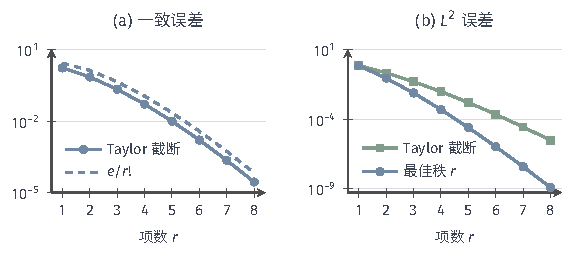
\includegraphics[width=95.9mm]{figures/02-abstract-mathematics/03-function-spaces/tikz/c6-lowrank-errors/figure.pdf}
  \caption{$e^{xy}$在$[-1,1]^2$上的$r$项分离逼近，对数纵轴。(a)~Taylor截断$E_r$的一致误差（实线）与上界$e/r!$（虚线）。(b)~$L^2$误差：Taylor截断（方块）与最佳秩$r$截断（圆点），后者由Legendre正交基下系数矩阵的奇异值算出，为$(\sum_{j>r}\sigma_j^2)^{1/2}$。可行的构造不一定最优。}
  \label{fig:apx-lowrank-errors}
\end{figure}

\paragraph{非正交基与Gram矩阵}

上面的结论依赖基的正交性。若$\bm\varphi$、$\bm\psi$不正交，记Gram矩阵$\bm G_\varphi=[\langle\varphi_i,\varphi_{i'}\rangle]$、$\bm G_\psi=[\langle\psi_k,\psi_{k'}\rangle]$，由式~\eqref{eq:apx-coefficient-matrix}和式~\eqref{eq:apx-product-inner}，
\[
  \|F\|^2=\int\!\!\int\bm\varphi^{\top}\bm C\bm\psi\bm\psi^{\top}\bm C^{\top}\bm\varphi\,\mathrm d\mu\,\mathrm d\nu
  =\operatorname{tr}\bigl(\bm C\bm G_\psi\bm C^{\top}\bm G_\varphi\bigr)
  =\bigl\|\bm G_\varphi^{1/2}\bm C\bm G_\psi^{1/2}\bigr\|_F^2 .
\]
因此最佳截断应作用于加权矩阵$\bm G_\varphi^{1/2}\bm C\bm G_\psi^{1/2}$，截断后再变换回原系数；直接截断$\bm C$的奇异值分解，一般不是$L^2$最优的。

$e^{xy}$恰好是一个例子。在单项式基$\{1,x,x^2,\ldots\}$下，Taylor系数矩阵是对角阵$\operatorname{diag}(1,1,1/2!,1/3!,\ldots)$，它的截断奇异值分解正是Taylor截断$E_r$。单项式基不正交，所以这个截断不是最佳的，图~\ref{fig:apx-lowrank-errors}(b)中两条曲线的差距就来自这里。

\paragraph{项数、因子幅度与高阶情形}

项数$r$、因子的幅度和误差是三个不同的量。同一个乘积可以写成$u\otimes v=(\lambda u)\otimes(v/\lambda)$，因子的大小不由函数决定；两项之差$M\,u\otimes v-M\,u\otimes v'$在$v'$接近$v$时可以很小，而每个因子的范数都含有$M$。只给出项数，既不能控制输出的大小，也不能保证计算稳定。

两组变量的结论依赖矩阵的奇异值分解，不能直接推广到三组及以上的变量。考虑三元函数$T(x,y,z)=x+y+z$，令
\[
  T_n(x,y,z)=n\Bigl(1+\frac xn\Bigr)\Bigl(1+\frac yn\Bigr)\Bigl(1+\frac zn\Bigr)-n .
\]
展开得$T_n=T+(xy+yz+zx)/n+xyz/n^2$，在有界区域上一致收敛到$T$，而每个$T_n$只有两个乘积项（常数$-n$也是乘积函数）。另一方面，$T$不能写成两个三元乘积之和：把任一表示投影到每个变量的$\operatorname{span}\{1,x\}$上，问题化为$2\times2\times2$张量的秩，而对应张量的秩为$3$\scite{desilva2008tensor}。于是$T$到两项表示的距离为零却无法达到，最佳两项近似不存在；逼近列$T_n$的因子幅度还随$n$发散。高阶情形的低秩逼近需要专门的理论，不能套用矩阵截断公式。

% 第8章第3节：函数类的紧性与覆盖数（Arzelà--Ascoli判据、覆盖数与度量熵、覆盖数的估计）。

\section{函数类的紧性与覆盖数}
\label{sec:apx-function-classes}

前两节始终固定一个目标：先给定$f$，再为它挑选近似，近似的预算可以依赖$f$。现在改为预先给定一个函数类$\mathcal F$，要求一套有限的代表同时服务于类中所有成员。量词的次序随之改变：“对每个$f$，存在有限表示”与“存在一套有限代表，对每个$f$都有一个靠近它的代表”是两个不同的命题。后者成立与否，取决于所用的距离以及类中函数共同受到的幅度和正则性约束。

第~\ref{chap:linear-functionals-operators}章的弱紧性不能代替这里的判断。在无限维Hilbert空间中，标准正交序列$(e_n)$有界并弱收敛到零（第~\ref{sec:lfo-weak-subsequence}节），但$\|e_n-e_m\|=\sqrt2$（$n\ne m$），没有按范数收敛的子列，单位球也不能被有限个半径小于$\sqrt2/2$的球覆盖。弱拓扑下的紧性针对较弱的收敛方式；在一致距离或$L^2$距离下能否有限覆盖，需要另外判断。本节先刻画一致距离下的相对紧性，再计量覆盖所需代表的个数。

\subsection{一致有界与等度连续}
\label{sec:apx-arzela-ascoli}

\paragraph{有界不足以抽出一致收敛子列}

在有限维空间中，有界序列总有收敛子列。在$C([0,1])$中这一点不再成立。考虑$f_n(x)=x^n$，它们都满足$\|f_n\|_\infty=1$。逐点地看，$x\in[0,1)$时$x^n\to0$，而$f_n(1)=1$，逐点极限是在$x=1$处跳到$1$的不连续函数。若某个子列一致收敛，其极限连续（一致极限保持连续性，可参考\BookChapterRef{chap:limits-continuity}{卷一“极限与连续”章}），又必须等于逐点极限，这是矛盾。所以$(x^n)$没有一致收敛的子列。

图~\ref{fig:apx-xn-powers}显示了问题出在哪里：$n$越大，函数在$x=1$附近从接近$0$升到$1$所用的区间越窄。每个$x^n$各自连续，但它们的连续性尺度没有共同的下界。

\begin{figure}[!htb]
  \centering
  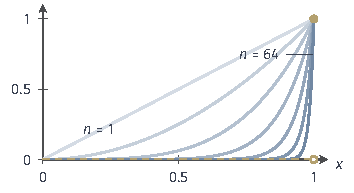
\includegraphics[width=60.0mm]{figures/02-abstract-mathematics/03-function-spaces/tikz/c6-xn-powers/figure.pdf}
  \caption{$[0,1]$上的$x^n$，$n=1,2,4,\ldots,64$（颜色由浅到深）。函数族一致有界，逐点极限在$[0,1)$上为$0$、在$x=1$处为$1$（黄色），不连续，因此没有一致收敛的子列；陡升区间随$n$变窄，族缺少共同的连续性尺度。}
  \label{fig:apx-xn-powers}
\end{figure}

\paragraph{等度连续}

缺少的条件是整个族共用一个连续性尺度。

\begin{definition}[一致有界与等度连续]
\label{def:apx-equicontinuous}
设$(X,d)$是度量空间，$\mathcal F$是$X$上的一族实值函数。若存在$M$使$|f(x)|\le M$对所有$f\in\mathcal F$、$x\in X$成立，称$\mathcal F$\term{一致有界}（uniformly bounded）。若对每个$\varepsilon>0$存在$\delta>0$，使
\[
  d(x,y)<\delta\ \Longrightarrow\ |f(x)-f(y)|<\varepsilon\qquad\text{对所有}f\in\mathcal F,
\]
称$\mathcal F$\term{等度连续}（equicontinuous）。
\end{definition}

与单个函数的一致连续相比，关键在于$\delta$只依赖$\varepsilon$，不依赖$f$。用连续模的语言，等度连续就是$\sup_{f\in\mathcal F}\omega_f(\delta)\to0$。最常见的例子是共用一个Lipschitz常数的族：若每个$f\in\mathcal F$都满足$|f(x)-f(y)|\le Ld(x,y)$，取$\delta=\varepsilon/L$即可。

反例来自没有共同尺度的族。$(x^n)$不等度连续：对任意$\delta\in(0,1)$，取$x=1$、$y=1-\delta/2$，则$|f_n(x)-f_n(y)|=1-(1-\delta/2)^n\to1$。图~\ref{fig:apx-equicontinuity}比较了两族函数在同一个宽$0.1$的窗口内的振幅：(a)中四个函数的Lipschitz常数都是$0.8\pi$，窗口内振幅都不超过$0.26$；(b)中$0.5+0.5\sin(2\pi nx)$的频率增长，$n=16$时在窗口内已扫过整个$[0,1]$。

\begin{figure}[!htb]
  \centering
  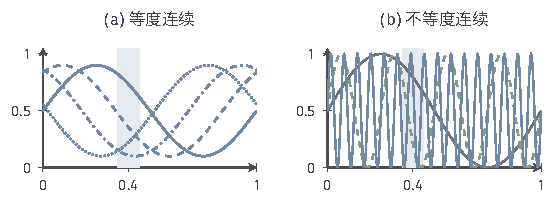
\includegraphics[width=94.2mm]{figures/02-abstract-mathematics/03-function-spaces/tikz/c6-equicontinuity/figure.pdf}
  \caption{共同连续性尺度的有无。蓝底为窗口$[0.35,0.45]$。(a)~$0.5+0.4\sin(2\pi x+a)$，$a=0,1,2,3$，共用Lipschitz常数$0.8\pi$，窗口内振幅都不超过$0.26$，族等度连续。(b)~$0.5+0.5\sin(2\pi nx)$，$n=1,4,16$，频率越高窗口内振幅越大，$n=16$时已达到$1$，族不等度连续。}
  \label{fig:apx-equicontinuity}
\end{figure}

\paragraph{Arzelà--Ascoli判据}

在紧度量空间上，一致有界与等度连续恰好刻画了一致距离下的相对紧性。回忆$C(X)$在一致范数下完备（第~\ref{sec:fs-uniform-norm}节）；子集称为\term{相对紧}（relatively compact），若它的闭包是紧集。

\begin{theorem}[Arzelà--Ascoli判据]
\label{thm:apx-arzela-ascoli}
设$(X,d)$是非空紧度量空间，$\mathcal F\subseteq C(X)$。则$\mathcal F$在一致范数下相对紧，当且仅当$\mathcal F$一致有界且等度连续。若$\mathcal F$还是闭集，则它是紧集。
\end{theorem}

证明的核心是一个有限化的机制：等度连续允许只在有限个位置上观察函数，一致有界允许把这些位置上的值量化为有限个等级，于是整个族只产生有限种“记录”。

\begin{proof}
充分性。设$|f|\le M$对所有$f\in\mathcal F$成立，并给定$\varepsilon>0$。由等度连续取$\delta>0$，使$d(x,y)<\delta$时$|f(x)-f(y)|<\varepsilon/4$对所有$f$成立。$X$紧，因而全有界，存在有限个点$x_1,\ldots,x_p$，使每个$x$都满足某个$d(x,x_i)<\delta$。再把$[-M,M]$分成有限个长度为$\varepsilon/4$的左闭右开小区间（最后一段含右端点），对每个$f$记下$f(x_1),\ldots,f(x_p)$各落在哪个小区间，称为$f$的记录。记录至多有$(\lceil8M/\varepsilon\rceil)^p$种，是有限个。

对每一种实际出现的记录，从$\mathcal F$中取一个具有该记录的成员作为代表。若$f$与代表$g$记录相同，则$|f(x_i)-g(x_i)|<\varepsilon/4$对每个$i$成立。对任意$x$取$x_i$使$d(x,x_i)<\delta$，
\[
  |f(x)-g(x)|\le|f(x)-f(x_i)|+|f(x_i)-g(x_i)|+|g(x_i)-g(x)|<\frac{3\varepsilon}4 .
\]
因此有限个代表构成$\mathcal F$的有限$\varepsilon$网，$\mathcal F$全有界。全有界集的闭包仍全有界（把每个球的半径放大一倍即可），而闭包是完备空间$C(X)$的闭子集，因而完备。由定理~\ref{thm:metric-compact-complete-tb}，闭包紧致。

必要性。设$\overline{\mathcal F}$紧，则$\mathcal F$全有界。取有限$\varepsilon/3$网$f_1,\ldots,f_N\in\mathcal F$。有界性：每个$f$都在某个$f_j$的$\varepsilon/3$邻域内，故$\|f\|_\infty\le\max_j\|f_j\|_\infty+\varepsilon/3$。等度连续：每个$f_j$在紧集上一致连续（定理~\ref{thm:metric-compact-uniform}），取$\delta$对这有限个函数同时适用，使$d(x,y)<\delta$时$|f_j(x)-f_j(y)|<\varepsilon/3$。对任意$f$选$f_j$使$\|f-f_j\|_\infty<\varepsilon/3$，则
\[
  |f(x)-f(y)|\le|f(x)-f_j(x)|+|f_j(x)-f_j(y)|+|f_j(y)-f(y)|<\varepsilon .
\]
最后，若$\mathcal F$闭，则$\mathcal F=\overline{\mathcal F}$紧。
\end{proof}

必要性的论证说明了有限网的作用：有限个函数总能共用一个$\delta$，再借助一致距离把这个$\delta$传给整个族。充分性中的位置网格和数值量化则是一个可以计数的构造，第~\ref{sec:apx-covering-estimates}节将用它给出Lipschitz类覆盖数的显式上界，图~\ref{fig:apx-lipschitz-quantization}画出了这个构造。

\paragraph{核范数有界球的一致紧性}

第~\ref{chap:rkhs}章的两个不等式恰好提供了Arzelà--Ascoli判据的两个条件。设$X$是紧度量空间，$K$是$X$上的连续半正定核，$B_R=\{f\in H_K:\|f\|_{H_K}\le R\}$。

\begin{theorem}[核范数球在连续函数空间中的紧性]
\label{thm:apx-rkhs-ball-compact}
在上述条件下，$B_R$是$C(X)$中按一致范数的紧集。
\end{theorem}

\begin{proof}
一致有界：由点值界（第~\ref{sec:rkhs-kernel-properties}节），$|f(x)|\le\|f\|_{H_K}\sqrt{K(x,x)}\le R\max_{X}\sqrt{K(x,x)}$，右端有限，因为连续函数在紧集上有最大值。

等度连续：由再生关系，
\[
  \begin{aligned}
  |f(x)-f(y)|&=|\langle f,K_x-K_y\rangle_{H_K}|\le R\,\|K_x-K_y\|_{H_K}\\
  &=R\sqrt{K(x,x)+K(y,y)-2K(x,y)} .
  \end{aligned}
\]
右端是$X\times X$上的连续函数，在对角线上为零。它在紧集$X\times X$上一致连续，所以存在$\delta$，使$d(x,y)<\delta$时右端小于$\varepsilon$，且$\delta$与$f\in B_R$无关。这里同时得到$B_R\subseteq C(X)$。

闭性：设$f_n\in B_R$且一致收敛到$g\in C(X)$。$(f_n)$在$H_K$中有界，由第~\ref{sec:lfo-weak-subsequence}节，存在子列弱收敛到某个$h\in H_K$；弱极限的范数不超过序列范数的下极限（第~\ref{sec:lfo-weak-norm}节），故$\|h\|_{H_K}\le R$。弱收敛蕴含$f_{n_k}(x)=\langle f_{n_k},K_x\rangle\to\langle h,K_x\rangle=h(x)$，而$f_{n_k}(x)\to g(x)$，所以$g=h\in B_R$。由定理~\ref{thm:apx-arzela-ascoli}，$B_R$紧。
\end{proof}

这个定理改变的是评价距离。$B_R$在一致距离下紧，并不意味着它在$H_K$自身的范数下紧：若$H_K$无限维，取其中的标准正交序列$(e_n)$，它们都在$B_1$中，彼此的核范数距离为$\sqrt2$，没有核范数收敛的子列。$[0,1]$上的高斯核就是这种情形：对互异中心$c_1,\ldots,c_M$，若$\sum_\ell a_\ell K_\sigma(\cdot,c_\ell)\equiv0$，乘以$e^{x^2/(2\sigma^2)}$后得到指数和$\sum_\ell a_\ell e^{-c_\ell^2/(2\sigma^2)}e^{c_\ell x/\sigma^2}\equiv0$，由引理~\ref{lem:apx-exponential-sum-zeros}全部$a_\ell=0$，所以$H_K$含有任意多个线性无关元素。

定理~\ref{thm:apx-rkhs-ball-compact}也补全了第~\ref{sec:apx-kernel-sections}节留下的论断：$B_R$在$C([0,1])$中闭且只含$H_K$的元素，$f_*\notin H_K$，所以$f_*$到$B_R$有正的一致距离。对任何固定的核范数预算$R$，有限核和都不能任意逼近$f_*$。

\subsection{覆盖数与度量熵}
\label{sec:apx-covering}

紧性回答“能否用有限个代表统一逼近”，没有回答“需要多少个”。本小节把代表的个数作为精度的函数记录下来。

\paragraph{覆盖数的定义与量词}

\begin{definition}[覆盖数与度量熵]
\label{def:apx-covering-number}
设$\mathcal F$是非空集合，$d$是$\mathcal F$上的距离或伪距离，$\varepsilon>0$。若有限集$V\subseteq\mathcal F$使每个$f\in\mathcal F$都有$v\in V$满足$d(f,v)\le\varepsilon$，称$V$为$\mathcal F$的一个$\varepsilon$覆盖。最小的覆盖规模
\[
  N(\varepsilon,\mathcal F,d)=\min\bigl\{|V|:V\text{是}\mathcal F\text{的}\varepsilon\text{覆盖}\bigr\}
\]
称为\term{覆盖数}（covering number），不存在有限覆盖时记为$+\infty$。其对数$\log N(\varepsilon,\mathcal F,d)$称为\term{度量熵}（metric entropy）。
\end{definition}

定义的量词是
\[
  \exists\ \text{有限}\ V\subseteq\mathcal F,\quad\forall f\in\mathcal F,\quad\exists v\in V:\ d(f,v)\le\varepsilon .
\]
代表集$V$必须在看到具体的$f$之前就固定下来，而且对类中每个成员都有效；只对大多数成员有效、或平均意义下有效，都不满足要求。每个$f$可以选择自己的近邻代表，但只能从$V$中选。

这里约定代表属于$\mathcal F$本身。若允许代表取自更大的空间，所得的外部覆盖数$N^{\mathrm{ext}}$可能更小，但两者只差精度的一个因子：
\[
  N^{\mathrm{ext}}(\varepsilon)\le N(\varepsilon)\le N^{\mathrm{ext}}(\varepsilon/2).
\]
第一个不等式显然。第二个：取一个外部$\varepsilon/2$覆盖，对每个与$\mathcal F$相交的球选一个类内成员替换球心，由三角不等式，原来落在该球中的成员到新代表的距离不超过$\varepsilon$。比较不同文献中的数值时，要先核对采用的是哪种约定。

\paragraph{覆盖数与全有界、紧性}

覆盖数把全有界的定义量化了。$\mathcal F$在$d$下全有界（定义~\ref{def:metric-totally-bounded}），当且仅当对每个$\varepsilon>0$都有$N(\varepsilon,\mathcal F,d)<\infty$：闭球$\{d(f,v)\le\varepsilon/2\}$含于开球$\{d(f,v)<\varepsilon\}$，开球又含于同半径的闭球，所以开球与闭球给出的有限性相同。若$\mathcal F$位于一个完备度量空间中，由定理~\ref{thm:metric-compact-complete-tb}，覆盖数处处有限等价于$\mathcal F$相对紧。结合定理~\ref{thm:apx-arzela-ascoli}，紧度量空间上一致有界且等度连续的函数族，在一致距离下对每个精度都有有限覆盖数。

伪距离允许$d(f,g)=0$而$f\ne g$。此时覆盖数只计及零距离等价类：彼此距离为零的成员共用同一个代表，因此应在第~\ref{sec:metric-pseudometric}节的商空间上理解覆盖数及其与紧性的关系。

\paragraph{三种距离的比较}

同一个函数类在不同距离下的覆盖数可以截然不同。设$X$上有概率测度$\mu$，又固定样本点$x_1,\ldots,x_n\in X$。三个常用的距离或伪距离为
\[
  \begin{aligned}
  d_\infty(f,g)&=\sup_{x\in X}|f(x)-g(x)|,\qquad
  d_{L^2(\mu)}(f,g)=\|f-g\|_{L^2(\mu)},\\
  d_n(f,g)&=\Bigl(\frac1n\sum_{i=1}^n\bigl(f(x_i)-g(x_i)\bigr)^2\Bigr)^{1/2}.
  \end{aligned}
\]
由于$\mu(X)=1$，后两者都不超过$d_\infty$。距离越弱，$\varepsilon$球越大，因此
\[
  N(\varepsilon,\mathcal F,d_{L^2(\mu)})\le N(\varepsilon,\mathcal F,d_\infty),\qquad
  N(\varepsilon,\mathcal F,d_n)\le N(\varepsilon,\mathcal F,d_\infty).
\]

经验距离$d_n$只看样本点，所以通常只是伪距离。图~\ref{fig:apx-empirical-distance}中$g(x)=0.3+0.4x$与$f(x)=g(x)+0.35\sin(5\pi x)$在六个样本点$0,0.2,\ldots,1$处取值相同，$d_n(f,g)=0$，但$d_\infty(f,g)=0.35$。

\begin{figure}[!htb]
  \centering
  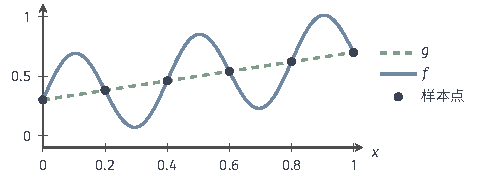
\includegraphics[width=81.2mm]{figures/02-abstract-mathematics/03-function-spaces/tikz/c6-empirical-distance/figure.pdf}
  \caption{经验距离只看样本点。$g(x)=0.3+0.4x$（虚线）与$f(x)=g(x)+0.35\sin(5\pi x)$（实线）在样本点$0,0.2,\ldots,1$（黑点）处相等，经验距离为$0$，一致距离却为$0.35$。}
  \label{fig:apx-empirical-distance}
\end{figure}

反方向的比较不成立，而且差距可以是有限与无穷之别。令$\mathcal F$为全体取值于$[0,1]$的连续函数。在$d_n$下，每个$f$由向量$(f(x_1),\ldots,f(x_n))\in[0,1]^n$决定距离；把每个坐标量化到$\lceil1/(2\varepsilon)\rceil$个等距点之一，所得网格点都是某个连续函数的样本值，于是$N(\varepsilon,\mathcal F,d_n)\le\lceil1/(2\varepsilon)\rceil^n<\infty$。在$d_\infty$下，取支撑互不相交的帽形函数列$(\phi_k)$，峰值为$1$，则$d_\infty(\phi_k,\phi_l)=1$（$k\ne l$），任何半径$1/3$的球至多含其中一个，所以$N(1/3,\mathcal F,d_\infty)=\infty$。样本上的记录有限，不能推出整个定义域上的有限覆盖；要从有限位置控制全域，需要等度连续这样的共同正则性，这正是定理~\ref{thm:apx-arzela-ascoli}的作用。

\subsection{覆盖数的估计与适用范围}
\label{sec:apx-covering-estimates}

本小节对几类具体的函数类估计覆盖数，观察它怎样依赖函数的幅度、参数维数、正则性和定义域。

\paragraph{常值族}

先看最简单的一维情形。设$X$非空，$M>0$，$\mathcal F_M=\{f_a\equiv a:a\in[0,M]\}$，距离取$d_\infty$。两个常值函数的距离就是$|a-a'|$，所以问题化为用半径$\varepsilon$的闭区间覆盖$[0,M]$。

下界由长度比较给出：每个代表$c$只覆盖长度为$2\varepsilon$的参数区间$[c-\varepsilon,c+\varepsilon]$，$N$个代表覆盖的总长度至多$2N\varepsilon$，必须不小于$M$。上界由均匀分点给出：令$N=\lceil M/(2\varepsilon)\rceil$，取$c_j=(2j-1)M/(2N)$，$j=1,\ldots,N$，相邻代表间距为$M/N\le2\varepsilon$，每个参数到最近代表的距离不超过$M/(2N)\le\varepsilon$。因此
\[
  N(\varepsilon,\mathcal F_M,d_\infty)=\Bigl\lceil\frac{M}{2\varepsilon}\Bigr\rceil,
\]
图~\ref{fig:apx-constant-cover}画出$M=1$、$\varepsilon=0.15$时的四个代表。

\begin{figure}[!htb]
  \centering
  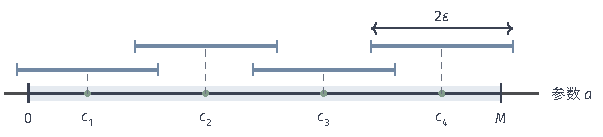
\includegraphics[width=102.2mm]{figures/02-abstract-mathematics/03-function-spaces/tikz/c6-constant-cover/figure.pdf}
  \caption{常值族$f_a\equiv a$（$a\in[0,1]$）在一致距离下的覆盖，精度$\varepsilon=0.15$。每个代表$c_j$（绿点）只覆盖长度$2\varepsilon$的参数区间（蓝色线段，上下错开以便辨认）；四个代表的总长度$1.2$不小于$1$，而三个只有$0.9$，所以覆盖数恰为$\lceil1/(2\varepsilon)\rceil=4$。}
  \label{fig:apx-constant-cover}
\end{figure}

这个例子已经显示了幅度的作用。参数个数固定为一个，把幅度$M$放大，覆盖数随$M$线性增长；一般地，对任意类$\mathcal F$和$B>0$，$N(\varepsilon,B\mathcal F,d_\infty)=N(\varepsilon/B,\mathcal F,d_\infty)$。度量熵$\log\lceil M/(2\varepsilon)\rceil$则只按$\log(1/\varepsilon)$增长。

\paragraph{有限维参数族}

再看两个参数的情形。设$\mathcal F=\{f_{a,b}(t)=a+bt:(a,b)\in[-1,1]^2\}$，$t\in[-1,1]$，距离取$d_\infty$。差$(a-a')+(b-b')t$是$t$的一次函数，绝对值的最大值在端点取得，等于$|a-a'|+|b-b'|$。因此一致距离恰好是系数平面上的$\ell^1$距离，$\varepsilon$球是菱形。

上界：把$[-1,1]$等分为$\lceil2/\varepsilon\rceil$段，取各段中点，每段长度不超过$\varepsilon$，所以每个坐标到最近中点的距离不超过$\varepsilon/2$。两个坐标方向的中点组成网格，每个系数点到最近网格点的$\ell^1$距离不超过$\varepsilon$，故$N(\varepsilon)\le\lceil2/\varepsilon\rceil^2$。下界：每个菱形面积为$2\varepsilon^2$，覆盖面积为$4$的正方形至少需要$4/(2\varepsilon^2)=2/\varepsilon^2$个。于是
\[
  \frac2{\varepsilon^2}\le N(\varepsilon,\mathcal F,d_\infty)\le\Bigl\lceil\frac2\varepsilon\Bigr\rceil^2,
\]
覆盖数按$\varepsilon^{-2}$增长，指数$2$正是参数个数。图~\ref{fig:apx-covering-centers}画出$\varepsilon=1/2$时的$16$个代表：(a)是系数平面上的菱形覆盖，(b)是对应的函数。

\begin{figure}[!htb]
  \centering
  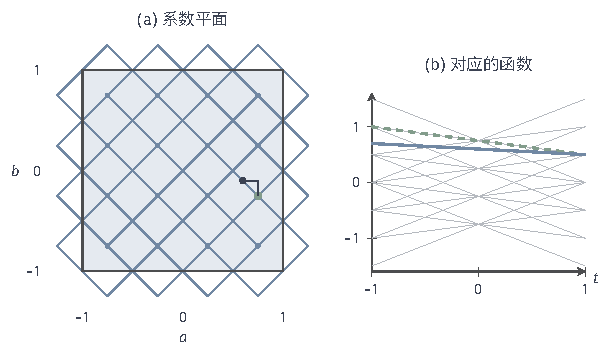
\includegraphics[width=103.2mm]{figures/02-abstract-mathematics/03-function-spaces/tikz/c6-covering-centers/figure.pdf}
  \caption{仿射函数类$a+bt$（$(a,b)\in[-1,1]^2$，$t\in[-1,1]$）的$\tfrac12$覆盖。(a)~一致距离等于系数的$\ell^1$距离，$16$个中心$\{\pm\frac14,\pm\frac34\}^2$的半径$\frac12$菱形覆盖整个正方形；黑点$(0.6,-0.1)$到最近中心$(\frac34,-\frac14)$（绿）的$\ell^1$距离为$0.3$。(b)~对应的函数：$16$条中心直线（细灰），成员$0.6-0.1t$（蓝）与其代表$0.75-0.25t$（绿虚线）的一致距离为$0.3$，在$t=-1$处取得。}
  \label{fig:apx-covering-centers}
\end{figure}

同样的论证适用于一般的有限维参数族。设$\mathcal F=\{\sum_{i=1}^p\theta_i\varphi_i:\|\bm\theta\|_\infty\le B\}$，$\varphi_i$有界，令$\Lambda=\sup_x\sum_i|\varphi_i(x)|$。则$d_\infty(f_{\bm\theta},f_{\bm\theta'})\le\Lambda\|\bm\theta-\bm\theta'\|_\infty$，把参数立方体$[-B,B]^p$在每个坐标上按精度$\varepsilon/\Lambda$分点，得到
\[
  N(\varepsilon,\mathcal F,d_\infty)\le\Bigl\lceil\frac{B\Lambda}\varepsilon\Bigr\rceil^p,\qquad
  \log N\le p\log\Bigl\lceil\frac{B\Lambda}\varepsilon\Bigr\rceil .
\]
若$\varphi_i$线性无关，有限维空间上的范数等价给出反方向的比较，再用体积论证可以得到同阶的下界，这里不展开。

\paragraph{参数个数不是覆盖数}

上面的例子中覆盖数的指数等于参数个数，但这是因为参数与函数一一对应且距离可以互相比较。覆盖数衡量的是函数集合本身在所选距离下的大小，与怎样参数化无关。把常值族改写成$f_{\theta_1,\theta_2}=\theta_1+\theta_2$，$\theta_1,\theta_2\in[0,M/2]$，参数变成两个，函数集合仍是$\{a:a\in[0,M]\}$，覆盖数不变。反过来，取$f_\theta\equiv\sin(M\theta)$，$\theta\in[0,2\pi]$，$M$为正整数：参数只有一个，参数到函数的映射随$M$增大而变得剧烈，但函数集合始终是取值于$[-1,1]$的常值函数，覆盖数$\lceil1/\varepsilon\rceil$与$M$无关。参数个数、参数化的剧烈程度和函数类的大小，是三个需要分别判断的量。

\paragraph{Lipschitz类的网格量化覆盖}

最后回到Arzelà--Ascoli判据证明中的构造，把它变成显式的计数。

\begin{theorem}[Lipschitz类的覆盖数上界]
\label{thm:apx-lipschitz-covering}
设$(X,d)$是非空紧度量空间，$L,M>0$，
\[
  \mathcal F_{L,M}=\bigl\{f:X\to\mathbb R:\ |f|\le M,\ |f(x)-f(y)|\le Ld(x,y)\bigr\}.
\]
则对每个$\varepsilon>0$，
\[
  N(\varepsilon,\mathcal F_{L,M},d_\infty)\le\Bigl\lceil\frac{4M}{\varepsilon}\Bigr\rceil^{p},\qquad
  p=N\Bigl(\frac{\varepsilon}{4L},X,d\Bigr).
\]
\end{theorem}

\begin{proof}
令$\delta=\varepsilon/(4L)$，$\eta=\varepsilon/2$。取$X$的一个$\delta$覆盖$x_1,\ldots,x_p$，使每个$x$都有$d(x,x_i)\le\delta$。把$[-M,M]$分成$\lceil2M/\eta\rceil=\lceil4M/\varepsilon\rceil$个长度不超过$\eta$的左闭右开小区间（最后一段含右端点），称$f$在各网格点处的值所在的小区间组成的序列为$f$的记录。记录至多有$\lceil4M/\varepsilon\rceil^p$种。

对每种实际出现的记录，取$\mathcal F_{L,M}$中一个具有该记录的成员作为代表。若$f$与代表$g$记录相同，则$|f(x_i)-g(x_i)|<\eta$。对任意$x$取$x_i$使$d(x,x_i)\le\delta$，
\[
  |f(x)-g(x)|\le Ld(x,x_i)+|f(x_i)-g(x_i)|+Ld(x_i,x)<2L\delta+\eta=\varepsilon .
\]
所以这些代表构成$\varepsilon$覆盖。
\end{proof}

图~\ref{fig:apx-lipschitz-quantization}以$L=1$、$M=0.6$、$\varepsilon=0.4$为例：$\delta=0.1$，网格点取$0.1,0.3,0.5,0.7,0.9$（$p=5$），值域按$\eta=0.2$分层，共$6$层，上界为$6^5=7776$。图中两个函数在每个网格点处落在同一层，一致距离约为$0.16$，不超过$0.4$。

\begin{figure}[!htb]
  \centering
  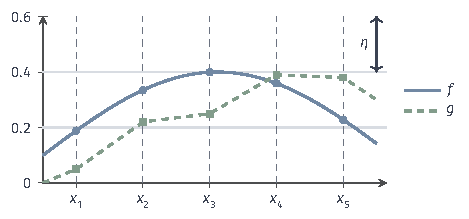
\includegraphics[width=79.4mm]{figures/02-abstract-mathematics/03-function-spaces/tikz/c6-lipschitz-quantization/figure.pdf}
  \caption{Lipschitz类的网格量化，$L=1$，$\varepsilon=0.4$。竖虚线为网格点$x_1,\ldots,x_5$，相邻间距$2\delta=0.2$，每点到最近网格点不超过$\delta=\varepsilon/(4L)$；横线把值域分为高$\eta=\varepsilon/2$的层（图中只画出非负部分）。$f(x)=0.1+0.3\sin3x$（蓝）与折线$g$（绿）在每个网格点处落在同一层，即记录相同，二者一致距离不超过$2L\delta+\eta=\varepsilon$。}
  \label{fig:apx-lipschitz-quantization}
\end{figure}

定义域的覆盖数出现在指数上。对$X=[0,1]$，$p=\lceil1/(2\delta)\rceil=\lceil2L/\varepsilon\rceil$，得到
\[
  \log N(\varepsilon,\mathcal F_{L,M},d_\infty)\le\Bigl\lceil\frac{2L}\varepsilon\Bigr\rceil\log\Bigl\lceil\frac{4M}\varepsilon\Bigr\rceil .
\]
与有限维参数族的$p\log(1/\varepsilon)$相比，这里的“有效维数”$\lceil2L/\varepsilon\rceil$随精度增长，Lipschitz类是无限维的。对$X=[0,1]^d$，网格点个数按$(L/\varepsilon)^d$增长，度量熵也随之增长，这是与张量积网格同源的维数效应。这个上界并不最优：Kolmogorov与Tikhomirov证明，固定$L$、$M$时，$[0,1]^d$上有界Lipschitz类的度量熵在$\varepsilon\to0$时与$\varepsilon^{-d}$同阶，上界中多出的对数因子可以去掉\scite{kolmogorov1959epsilon}。这里的构造只用来说明有限覆盖如何从共同的正则性和幅度约束中产生。

\paragraph{覆盖数之外的容量与保证}

覆盖数总是相对于一个预先固定的距离和精度定义的。学习理论中还会遇到其他容量量：伪维和胖打散维数检查一个类在有限输入上能实现多少种跨越阈值的模式，序贯覆盖数在依赖历史的查询树上计数。它们的评价对象与覆盖数不同，不能从名称相近而互换。覆盖数本身也不提供统计误差或预测保证；要得到这类结论，还需加入随机样本、损失函数和集中不等式，可参考\BookChapterRef{chap:statistical-learning-framework}{卷六“机器学习理论基础”章}。

% 第8章第4节：本章小结（同时收束“函数空间”部分）。

\section{本章小结}
\label{sec:apx-summary}

章首提出的三个问题，分别对应逼近对象的三个层次。

对一个给定的函数，逼近的含义取决于固定了什么：定义域、误差范数和生成单元。Bernstein多项式、线性样条、固定宽度的高斯核截面和单隐藏层网络都能一致逼近紧集上的任意连续目标，但这些都是可变预算下的存在性结论，次数、结点、中心或单元数随精度增加。误差随预算下降的速度另需光滑性：连续模给出$\omega_f(h)$量级，二阶导数有界给出$h^2$量级，折线$f_*$只有一阶。稠密性还不等于能稳定地算出系数：高斯核和的系数可能随精度发散，在固定核范数预算下甚至无法任意逼近$f_*$；网络参数也不可识别。

对多变量函数，乘积结构提供了组合的方式。在可分的$L^2$空间中，单变量正交基的乘积构成乘积测度下的正交基，张量积网格却使系数个数按$m^d$增长。低秩表示只保留少数乘积项；在正交基下，最佳$r$项$L^2$近似由系数矩阵的截断奇异值分解给出，非正交基须先计入Gram矩阵。项数、因子幅度与误差是不同的量，三组以上变量时最佳低秩近似甚至可能不存在。

对整个函数类，量词从“对每个目标存在近似”变为“存在一套代表适用于全体”。一致距离下，紧度量空间上的函数族相对紧，当且仅当一致有界且等度连续；核范数有界球因点值界与核截面差界而在$C(X)$中紧，却不在核范数下紧。覆盖数计量所需代表的个数，它依赖所选的距离：经验距离下的有限覆盖不能推出全域覆盖。常值族、有限维参数族与Lipschitz类的估计表明，覆盖数随幅度、参数维数、正则性和定义域维数变化，而不由参数个数单独决定。

至此，本部分建立了研究函数的几套工具：第~\ref{chap:function-spaces}章的范数、完备性与正交几何，第~\ref{chap:linear-functionals-operators}章与第~\ref{chap:operator-spectra-equations}章的泛函、算子、谱与方程，第~\ref{chap:weak-derivatives-sobolev}章以弱导数刻画的正则性，第~\ref{chap:rkhs}章以点值观测构造的核空间，以及本章的有限逼近与覆盖。它们回答的是候选函数在什么空间中、怎样度量、怎样表示和能逼近到什么程度。后续的优化问题在这些候选空间上加入目标函数与约束，研究最优解的存在、最优条件和求解方法，可参考\BookChapterRef{chap:optimization}{卷三“优化问题的定义与基本性质”章}；信号处理加入时间、频率和采样机制；统计与学习理论加入随机数据和误差保证。它们沿用这里已经确定的范数、表示与覆盖结论，只在各自的问题中补充新的结构。


